The first thing to realize when looking at the learning rate graphs of the models is that every line on the learning rate graph of OGLVQ models represents each prototype’s $\epsilon_{i}$ while in the CGLVQ model, it turns into class-based $\epsilon$. We did nothing different for learning rate graphs for the CGLVQ; the graph still shows the $\epsilon_{i}$ of each $\omega_{i}$, but every $\omega$ that shares the same class has the exact $\epsilon_{i}$. This observation is because, in standard GLVQ or OGLVQ, $\epsilon_{i}$ are updated for the $\omega^{+}$ and $\omega^{-}$ for that sample. However, in the CGLVQ models, $\epsilon$ update is based on classes. This $\epsilon$ update of CGLVQ happens because all of the $\omega_{i}$ in the same class share exact co-occurrence tables.

\section{Experiment 1 (Balanced Dataset)}

\subsection{Breast Cancer Wisconsin dataset}

Prototypes for each class: 3
\vspace{5pt}


The learning process reflects the models’ learning rate graph. The change in the learning rate graph indicates that the model adapts to a given dataset. We would like to see decreasing $\epsilon_{i}$ for all prototypes, which means the given model is learning positively. For \textit{Breast Cancer Wisconsin} dataset on experiment 1 with OGLVQ, every CGLVQ model except the CP model increases accuracy and decreases $\epsilon_{i}$ values, which brings positive learning as we can see the results of the models below. CGLVQ models shows good $\epsilon_{i}$ curves with low $\epsilon(0)$, 0.01. The CP model also shows positive learning at the beginning of the process with $\epsilon(0) = 0.01$ but decreases accuracy afterward and increases $\epsilon_{B}$ of class “Benign.” Still, CP is adapting to the model but not doing a good job regarding other models. Performance-wise, CGLVQ models except CP shows similar performance to OGLVQ.

Here is a small note to be careful about the axis of the given plots. With smaller $\epsilon(0)$, it is harder to visualize the motion of learning rates in the same scale as higher $\epsilon(0)$. So, the changes on the learning rate graphs do not reflect equal change with different ${\epsilon(0)}$. We investigate if there is a change in learning rates and, if so, in which direction.

\begin{figure}[H]
    \centering
    \begin{subfigure}[t]{0.45\textwidth}
        \centering
        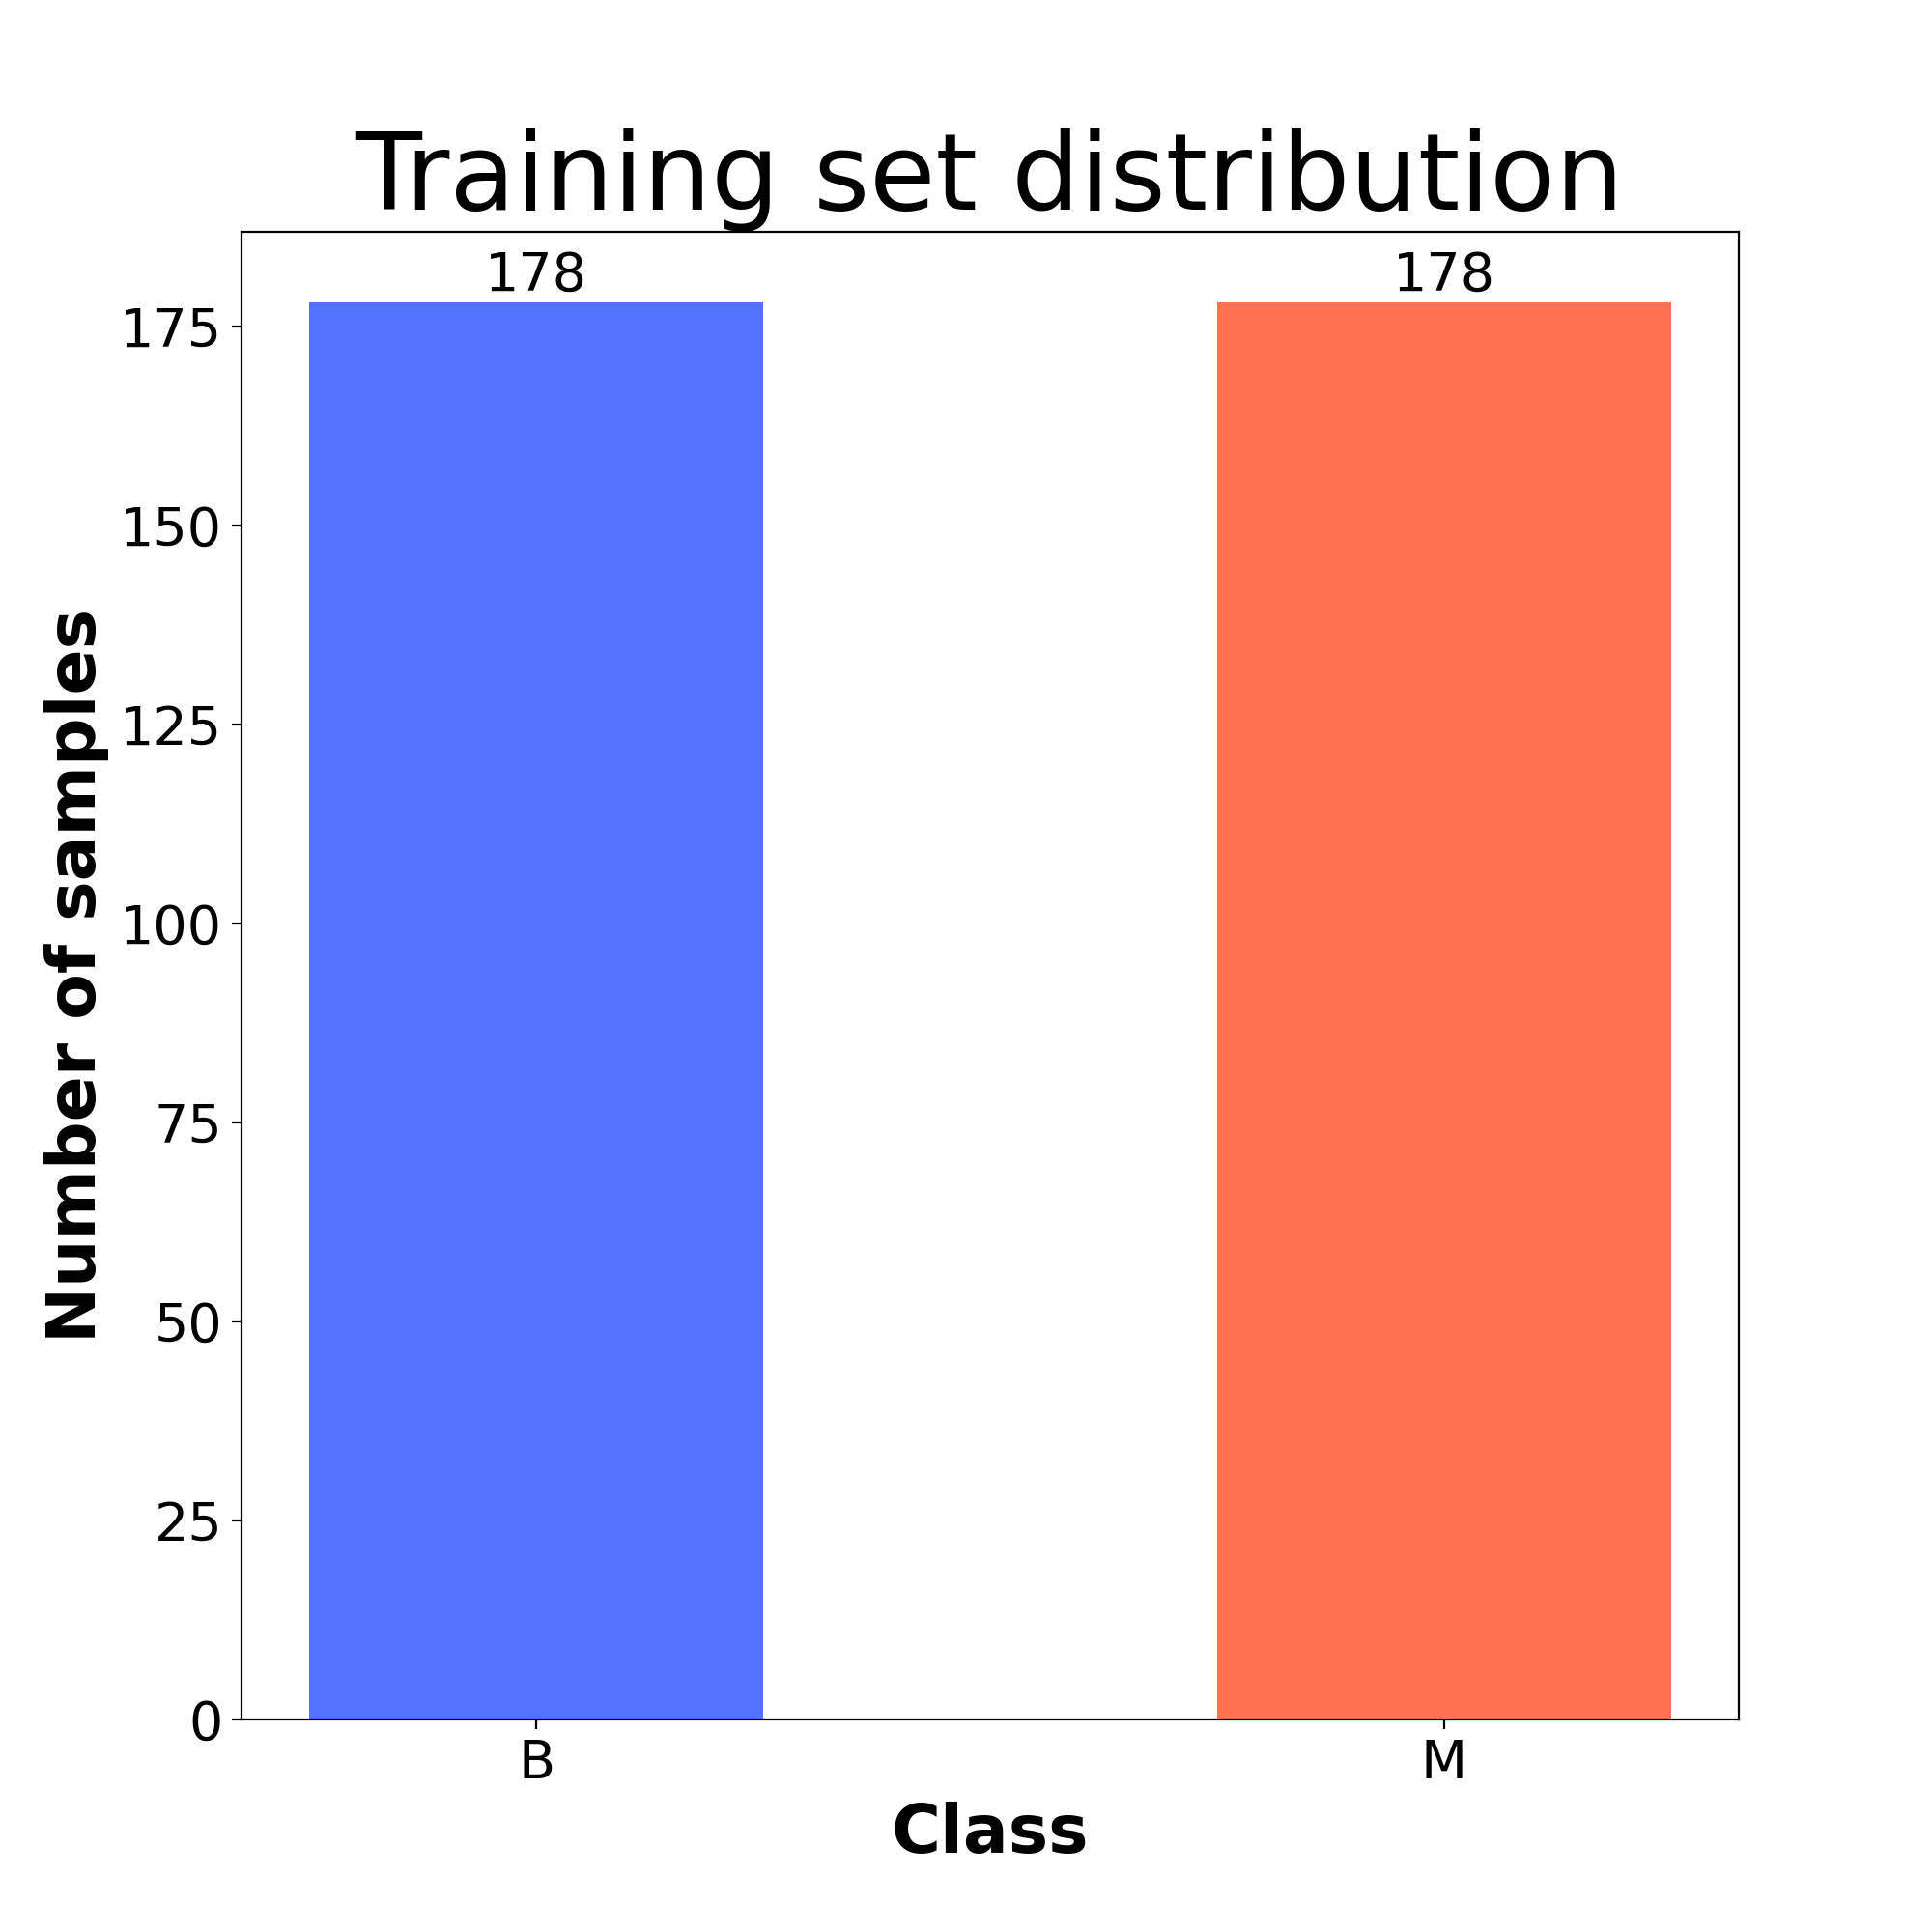
\includegraphics[width=1\textwidth]{images/exper1/breast/train_dist.png}
        \caption{Training set}
    \end{subfigure}
    \begin{subfigure}[t]{0.45\textwidth}
        \centering
        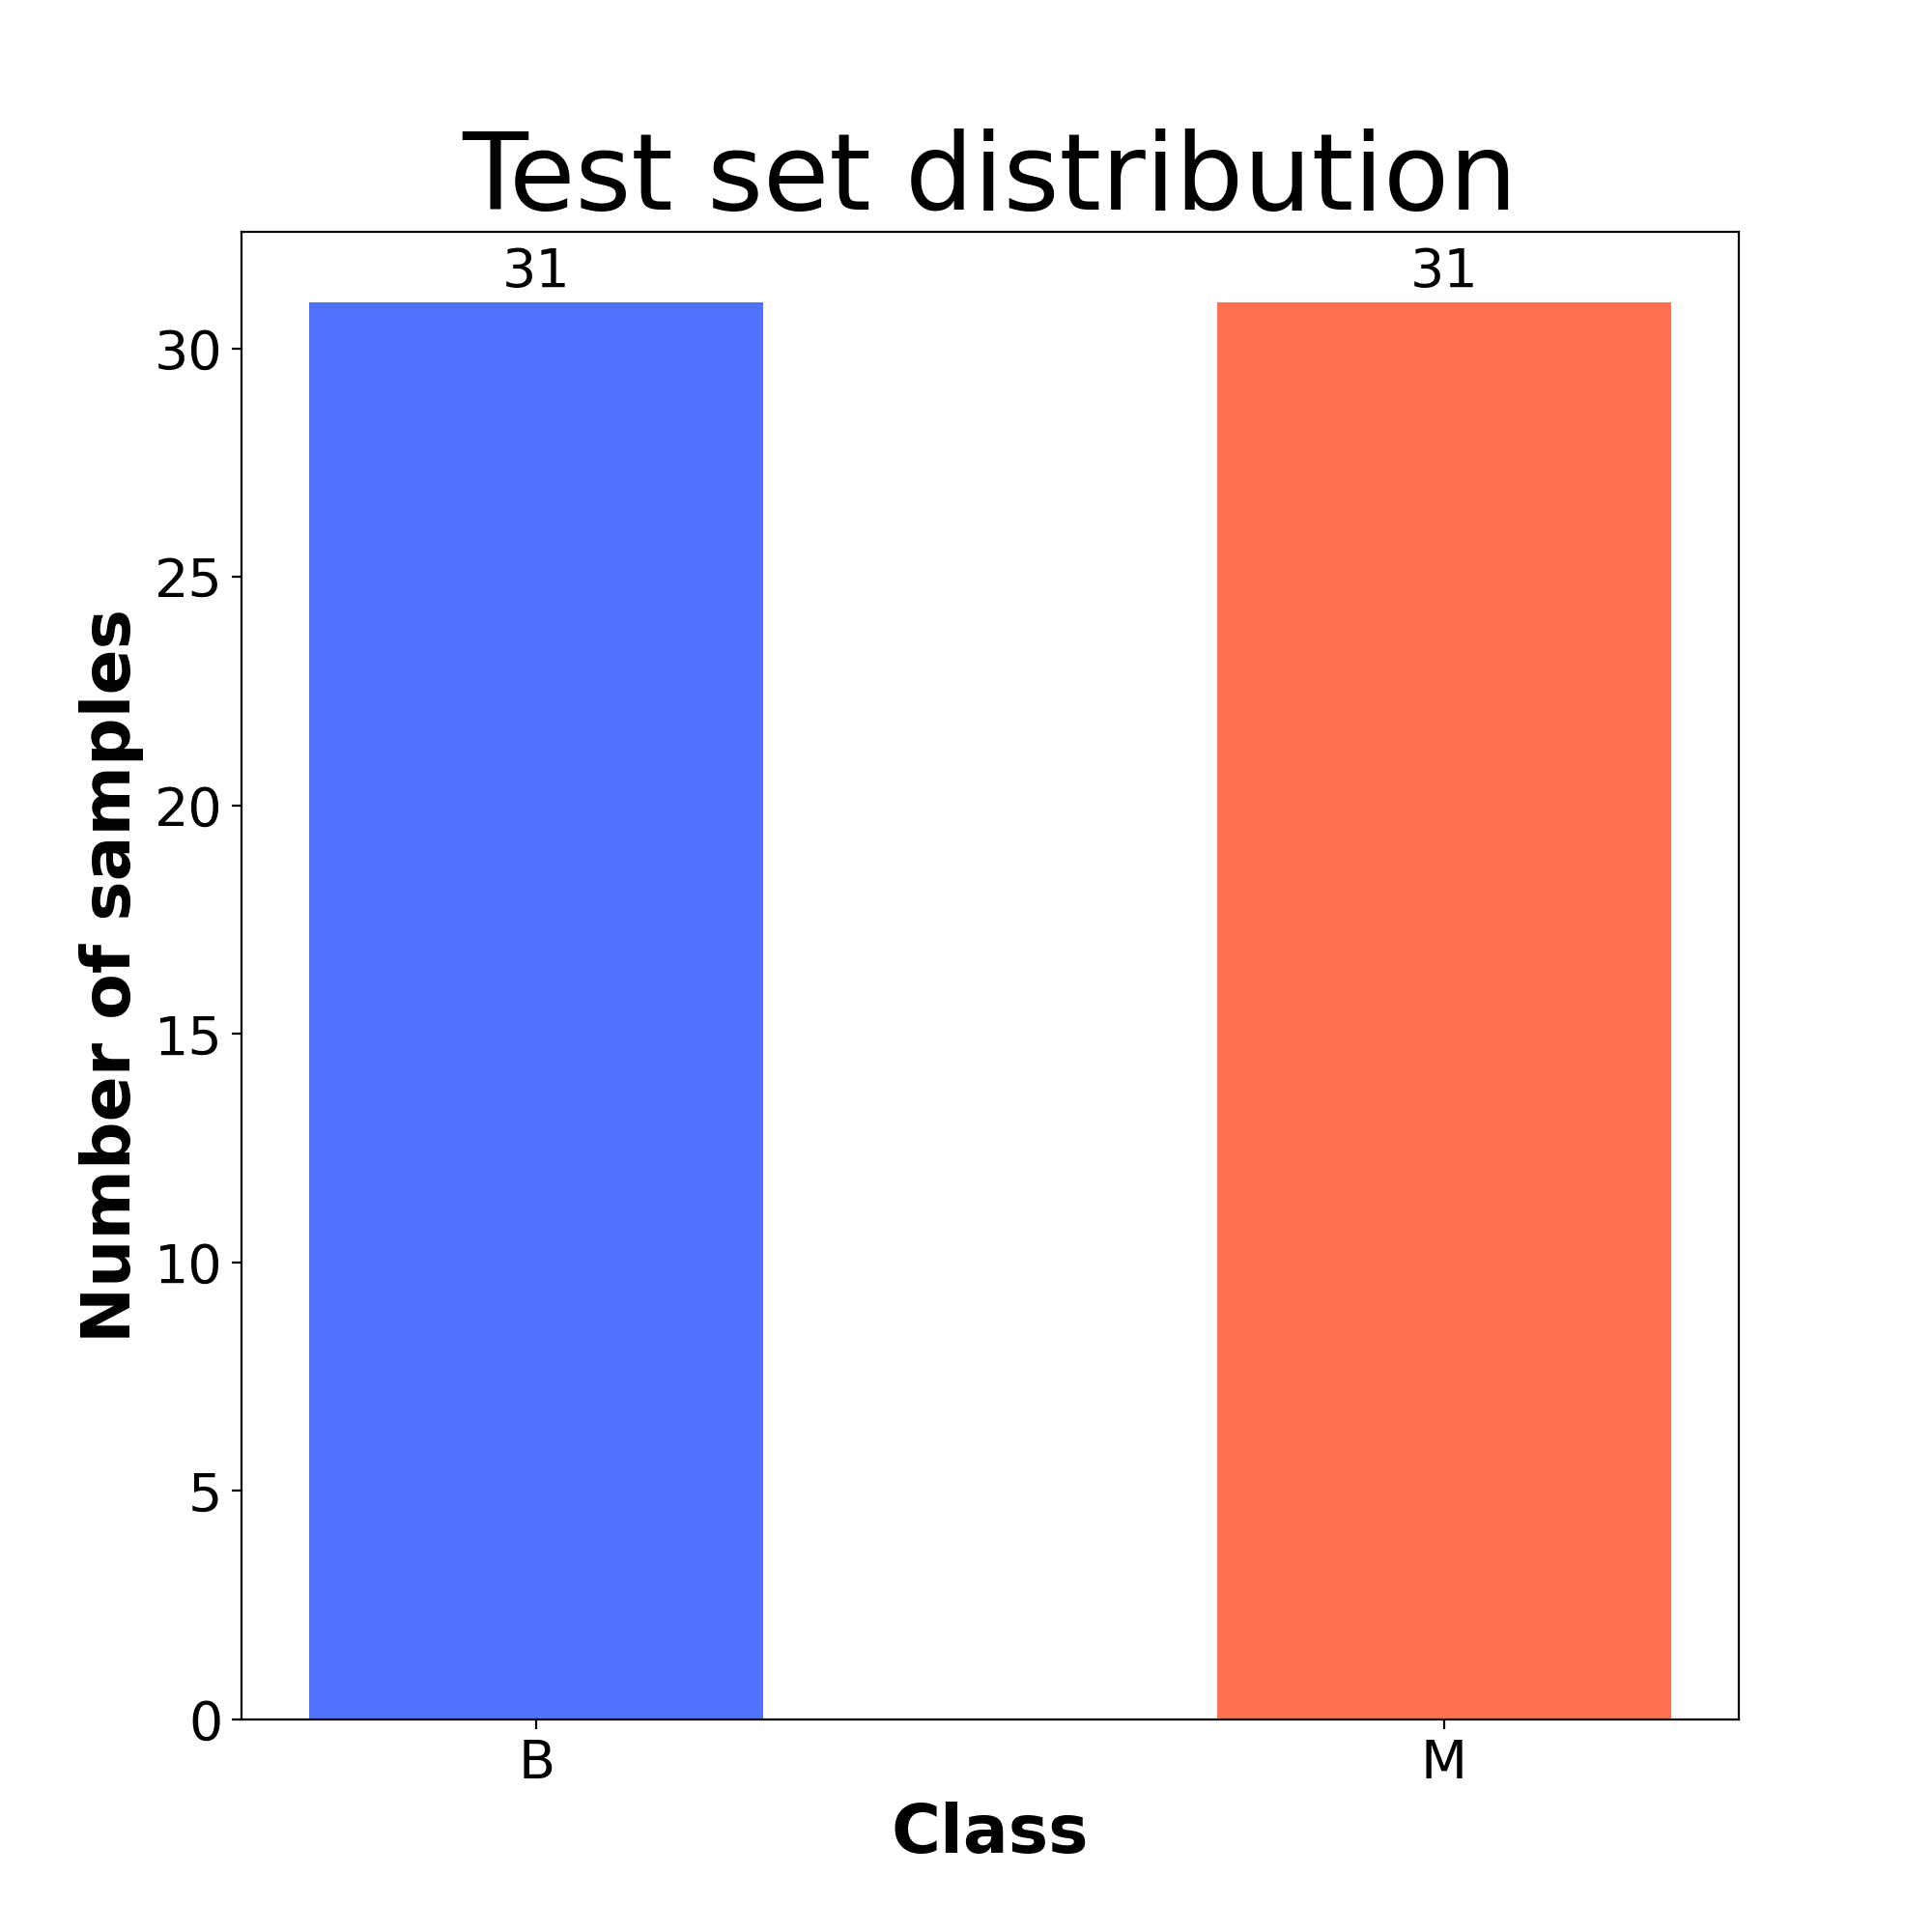
\includegraphics[width=1\textwidth]{images/exper1/breast/test_dist.png}
        \caption{Test set}
    \end{subfigure}
    \caption{\textit{Breast Cancer Wisconsin} balanced dataset sample distribution.}
\end{figure}

\begin{figure}[H]
    \centering % <-- added
\begin{subfigure}{0.3\textwidth}
  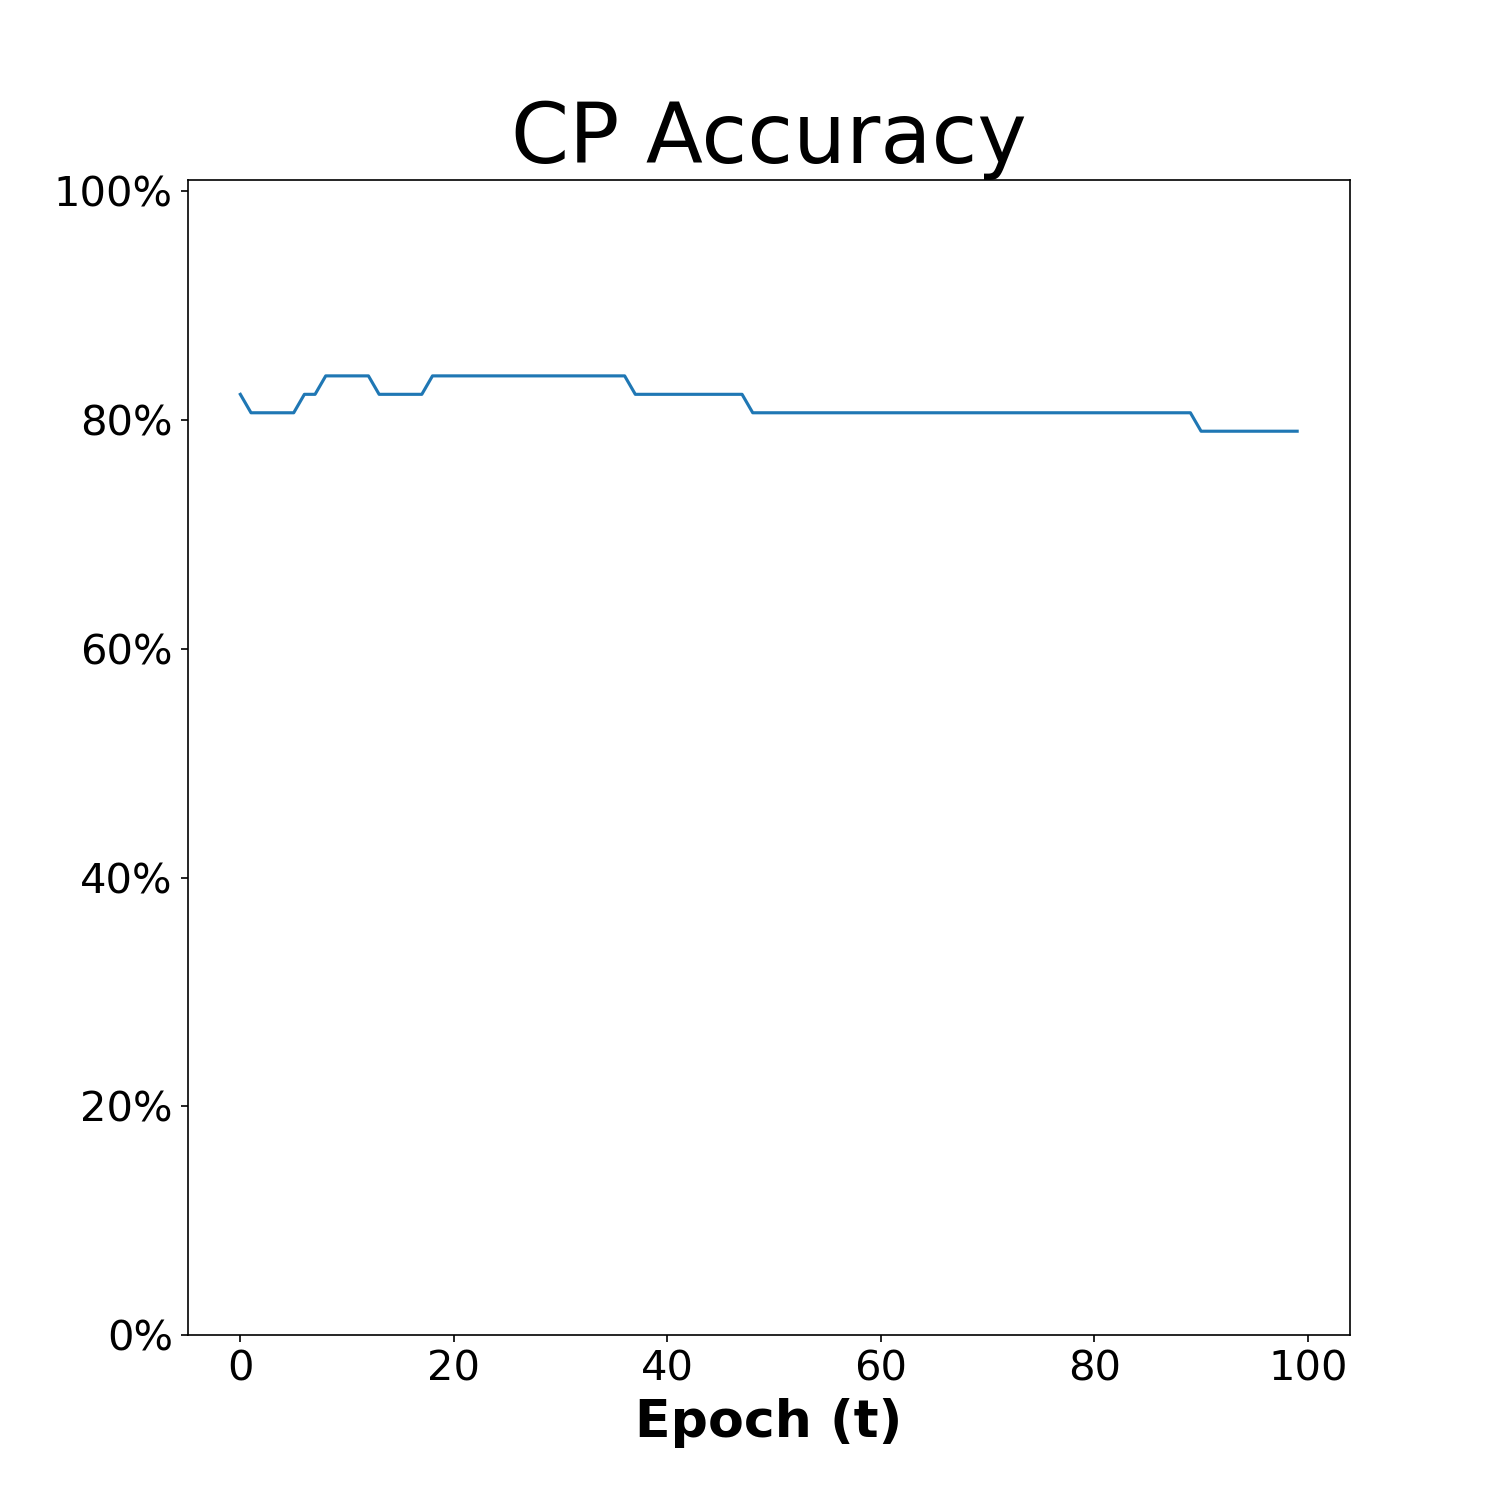
\includegraphics[width=\linewidth]{images/exper1/breast/CP_0.01_acc.png}
    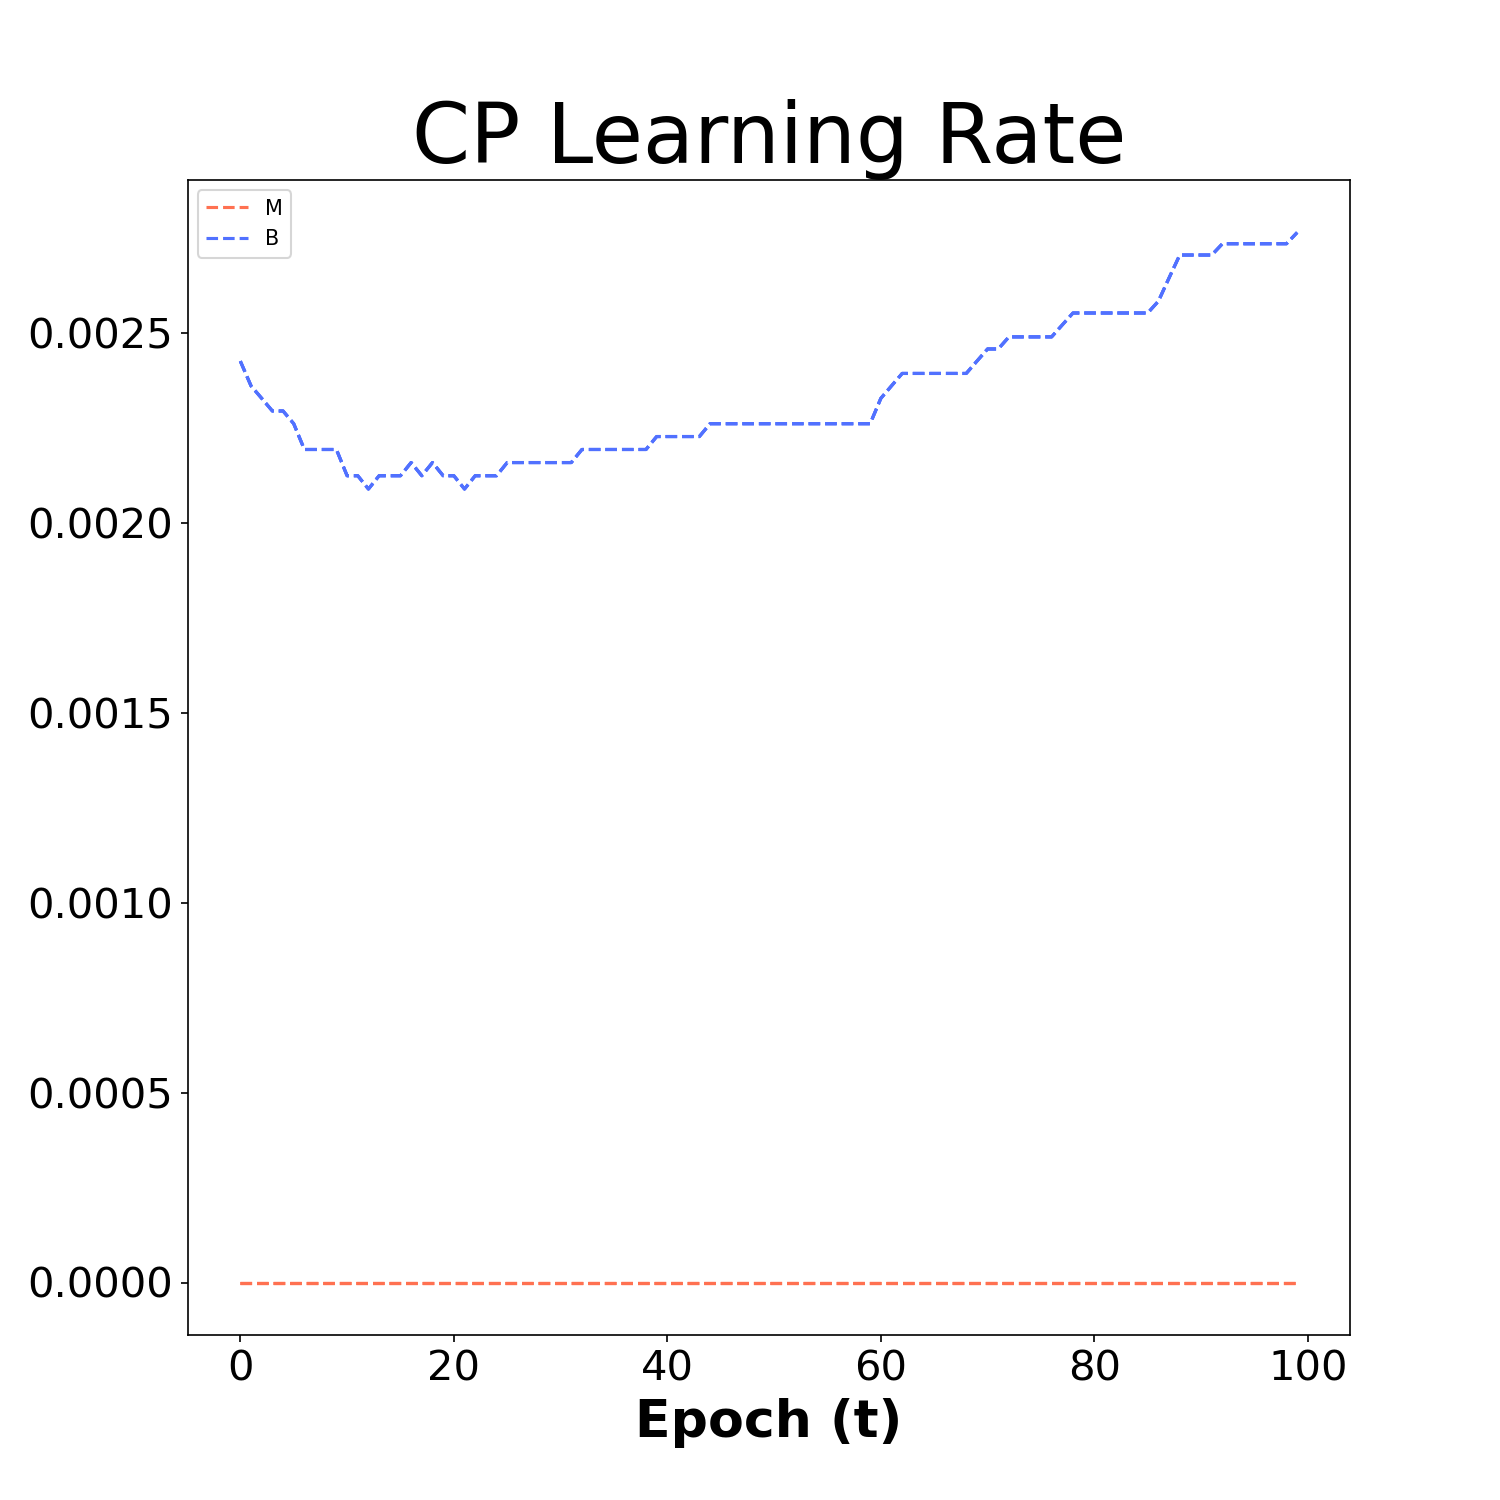
\includegraphics[width=\linewidth]{images/exper1/breast/CP_0.01_lr.png}
  \caption{$\epsilon(0)=0.01$}
\end{subfigure}\hfil % <-- added
\begin{subfigure}{0.3\textwidth}
  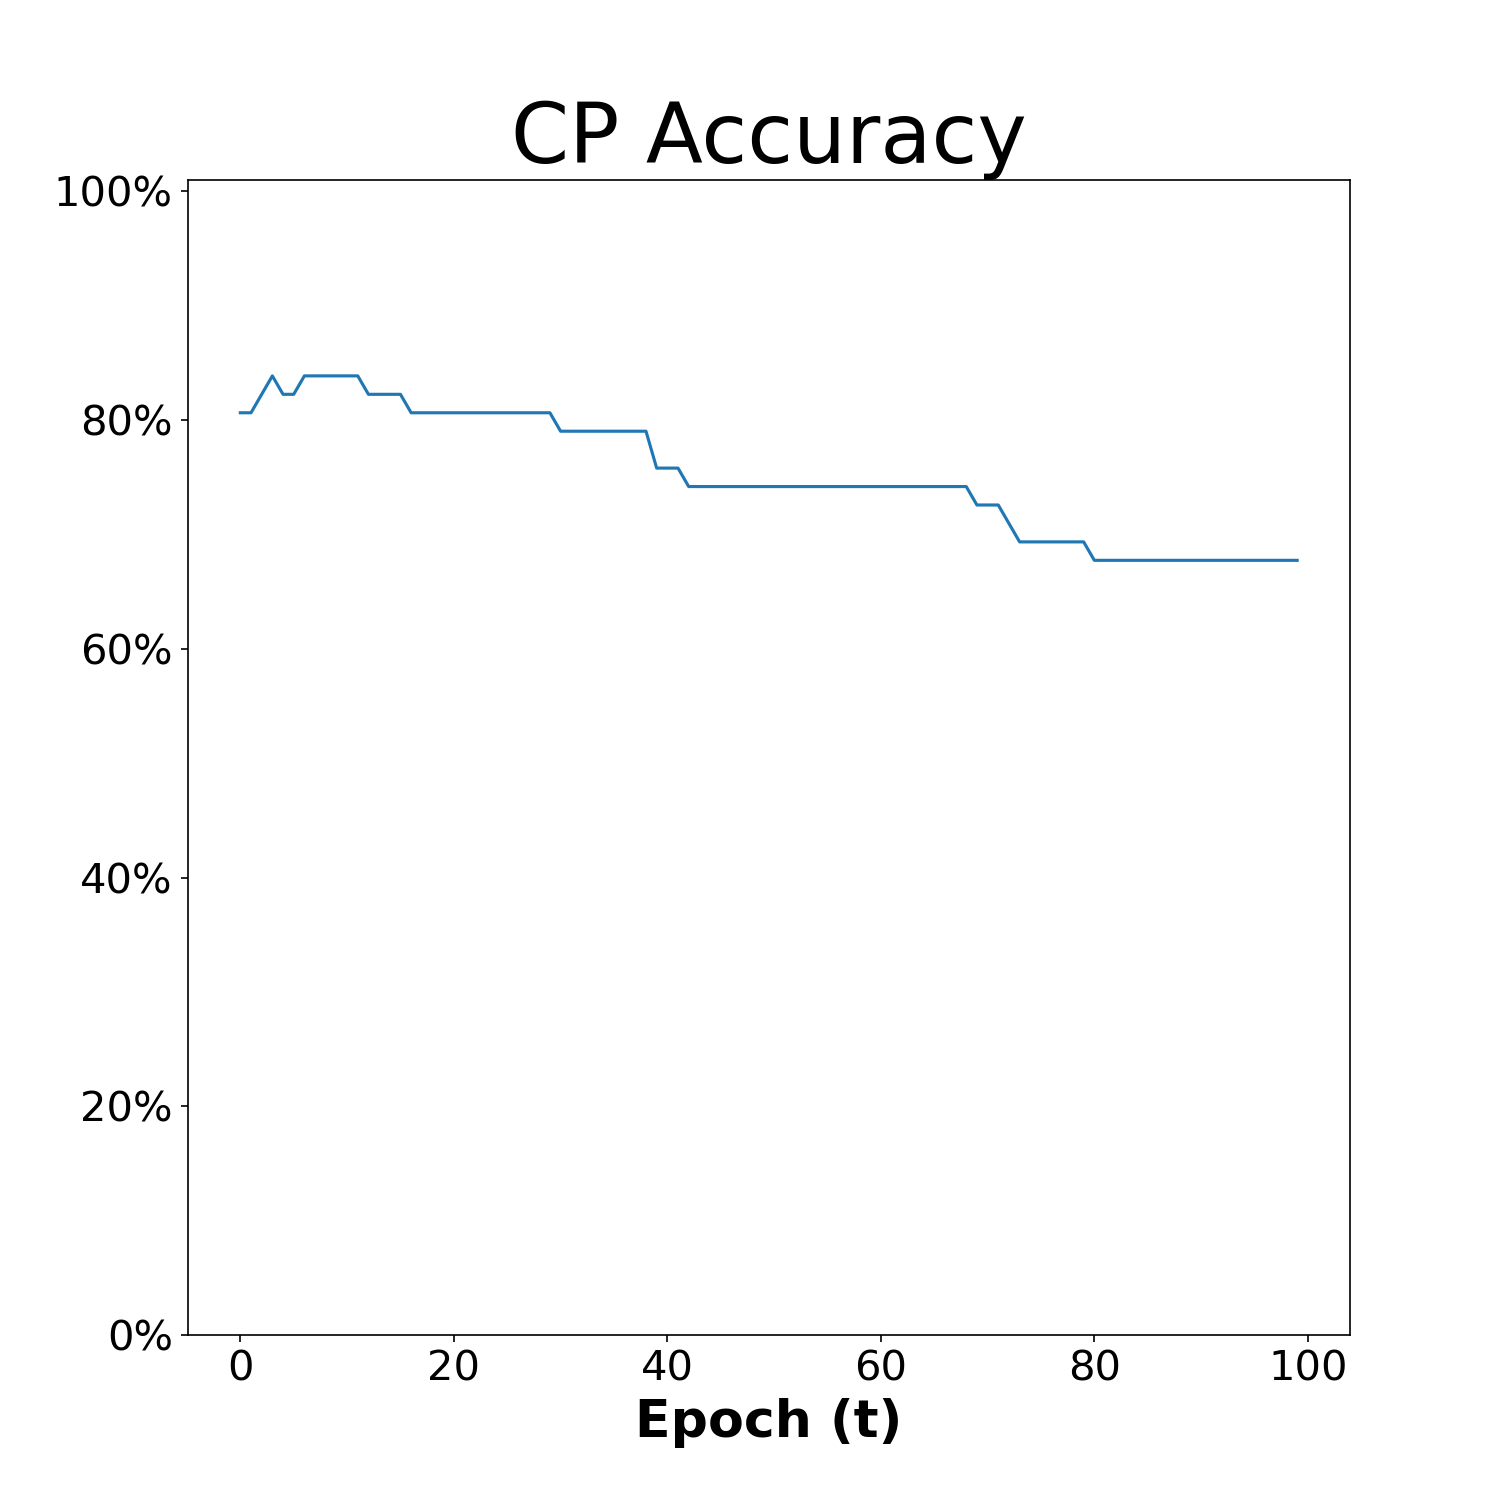
\includegraphics[width=\linewidth]{images/exper1/breast/CP_0.03_acc.png}
  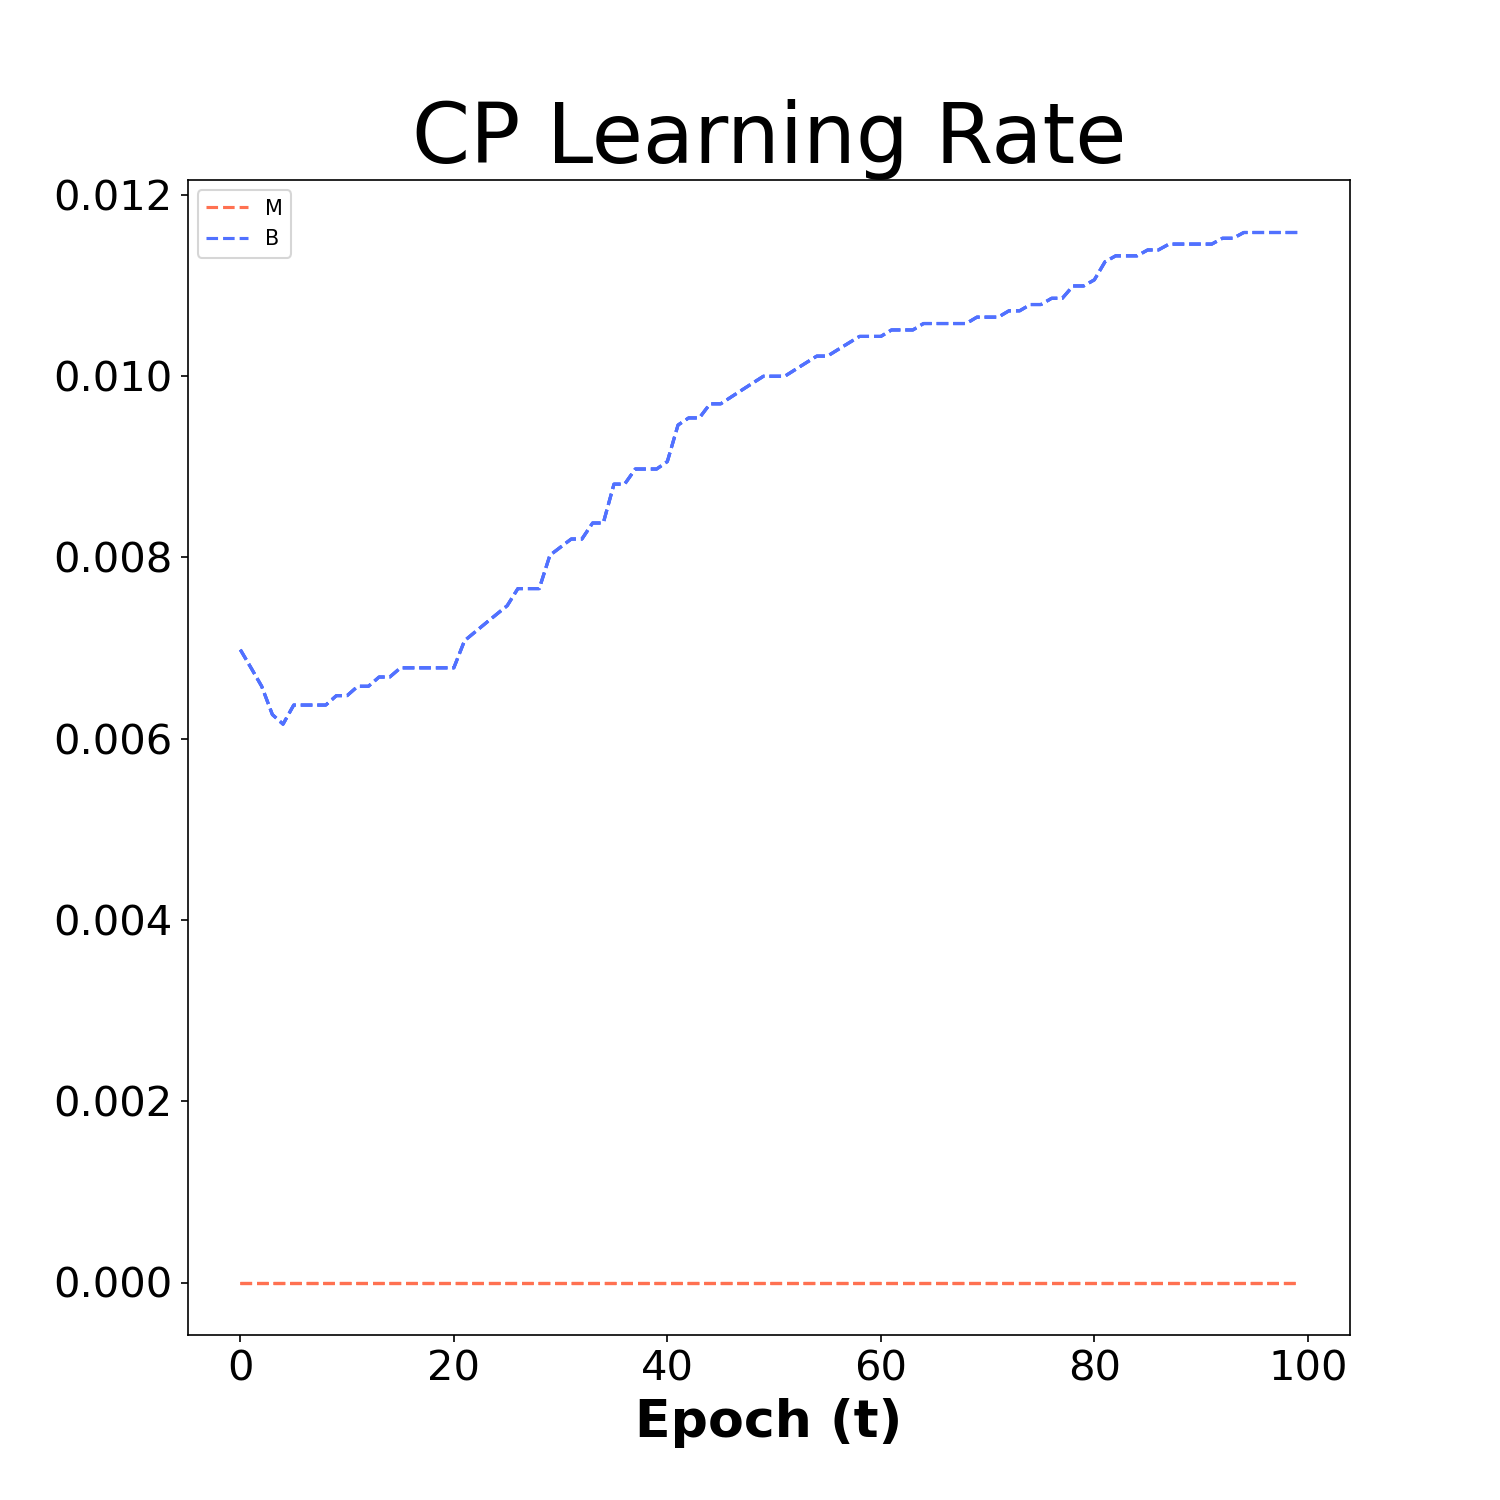
\includegraphics[width=\linewidth]{images/exper1/breast/CP_0.03_lr.png}
  \caption{$\epsilon(0)=0.03$}
\end{subfigure}\hfil % <-- added
\begin{subfigure}{0.3\textwidth}
  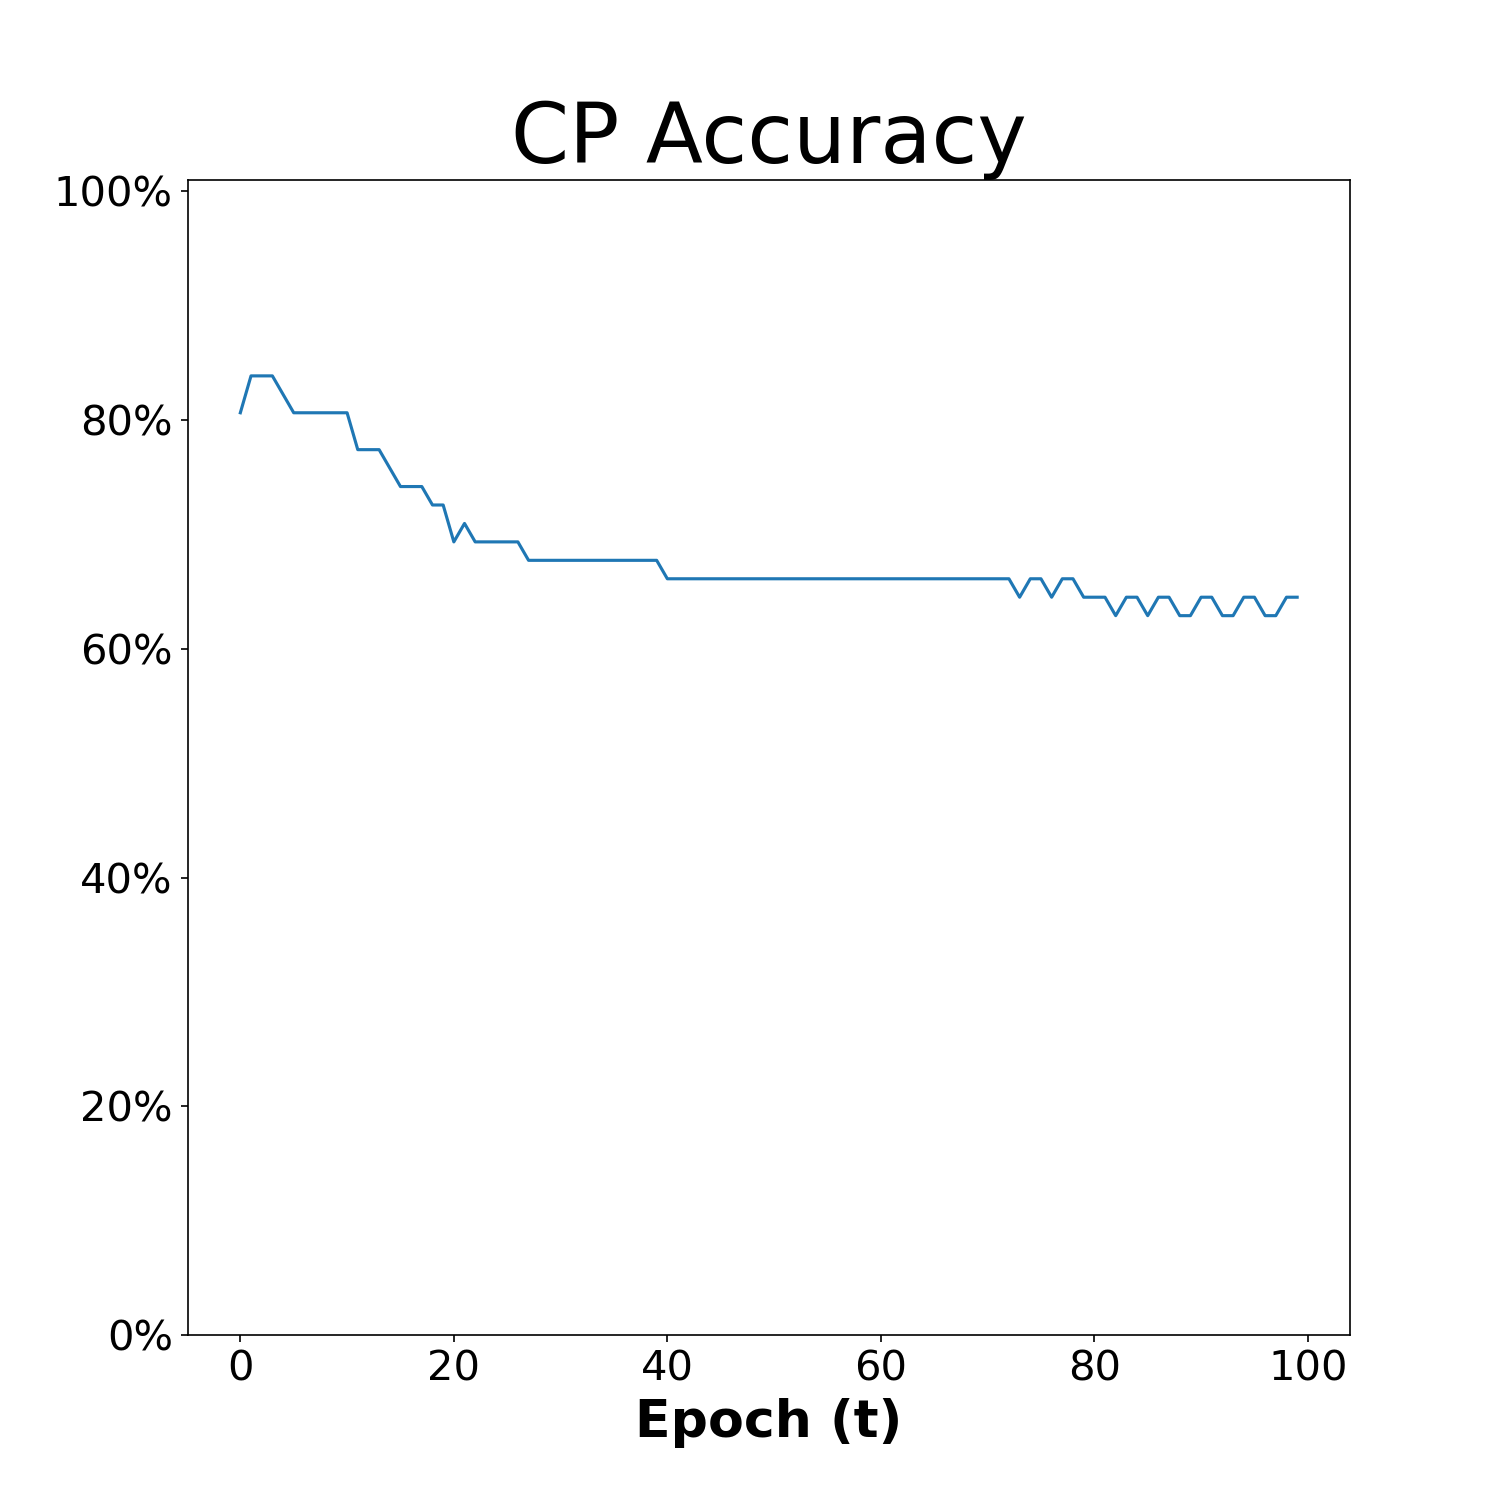
\includegraphics[width=\linewidth]{images/exper1/breast/CP_0.1_acc.png}
  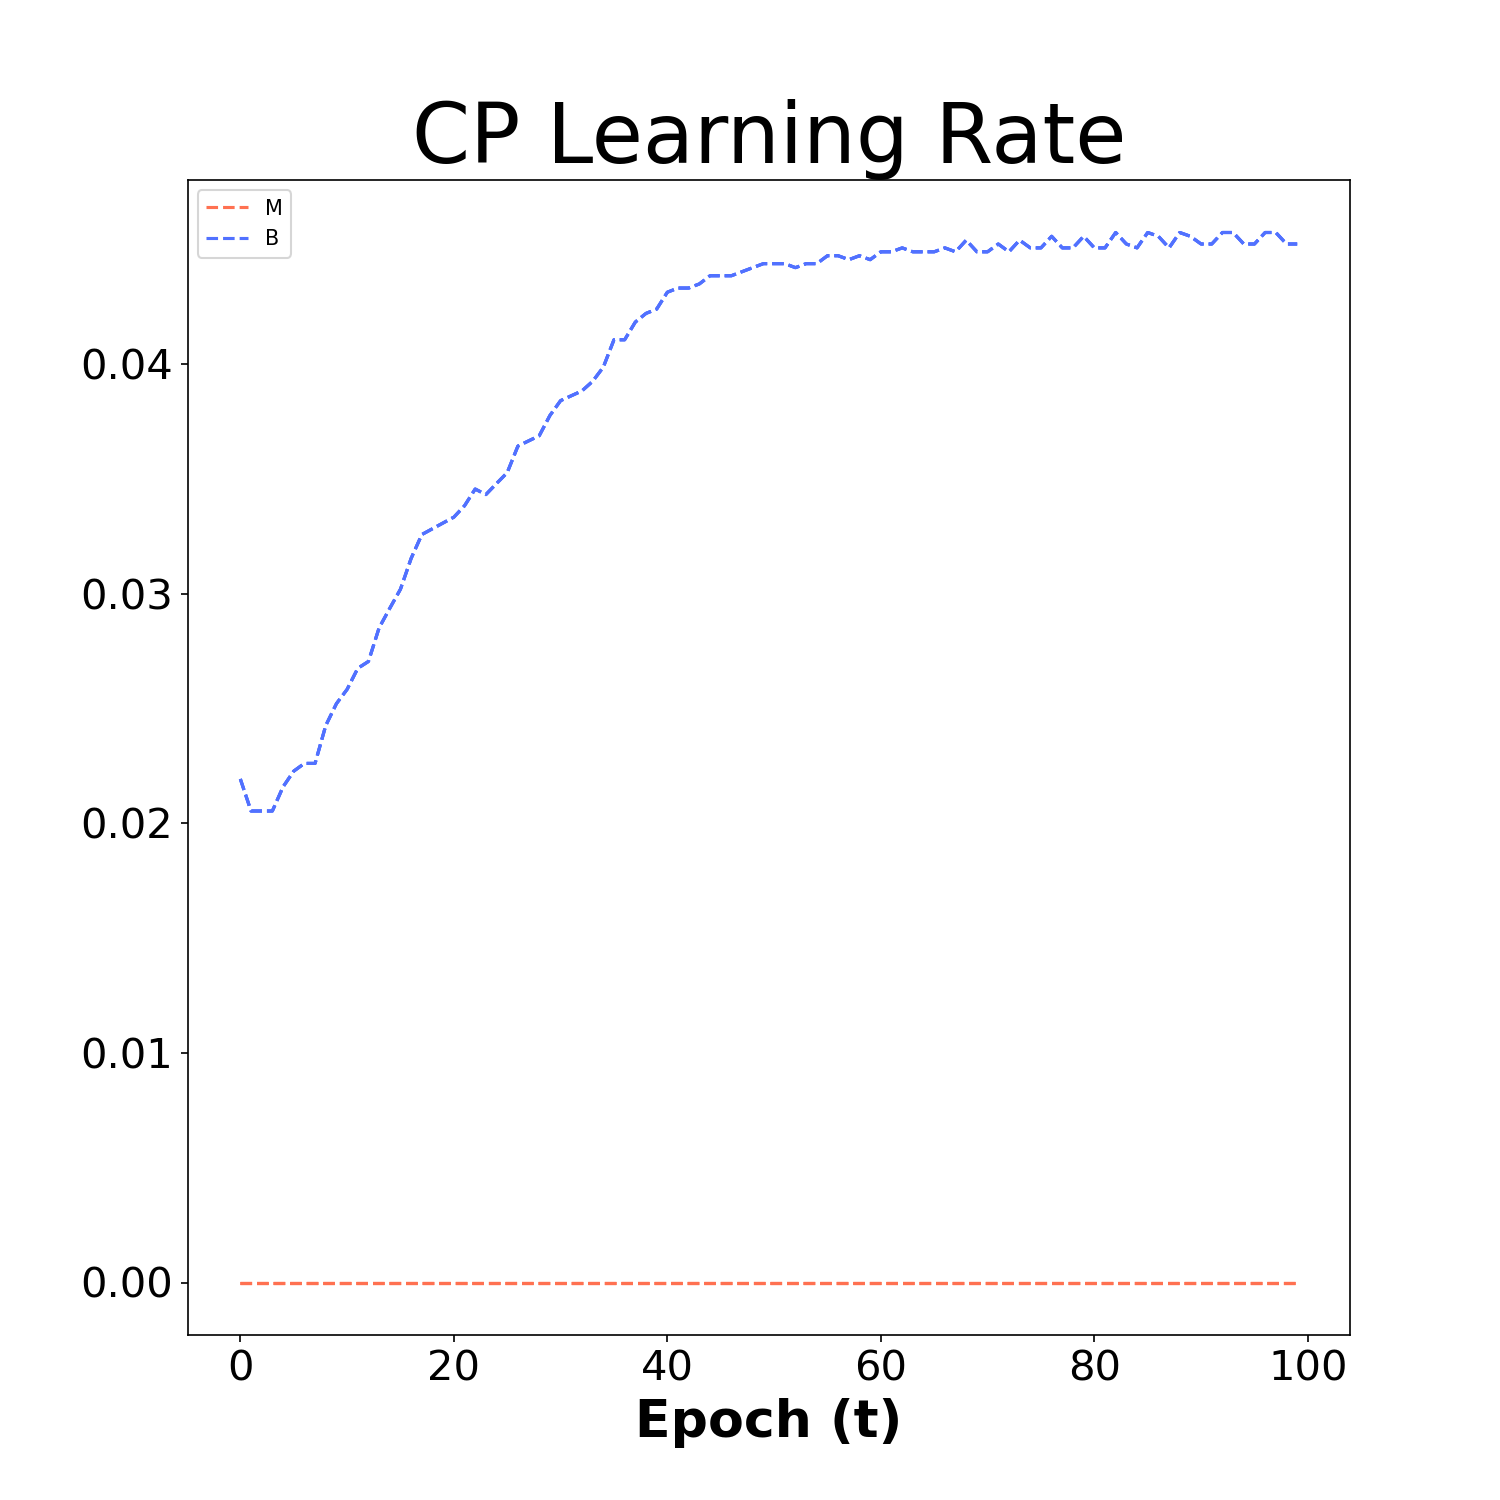
\includegraphics[width=\linewidth]{images/exper1/breast/CP_0.1_lr.png}
  \caption{$\epsilon(0)=0.1$}
\end{subfigure}

\caption{\textit{Breast Cancer Wisconsin} dataset accuracy score and learning rate results under CP model using balanced dataset.}
\end{figure}

\begin{figure}[H]
    \centering % <-- added
\begin{subfigure}{0.3\textwidth}
  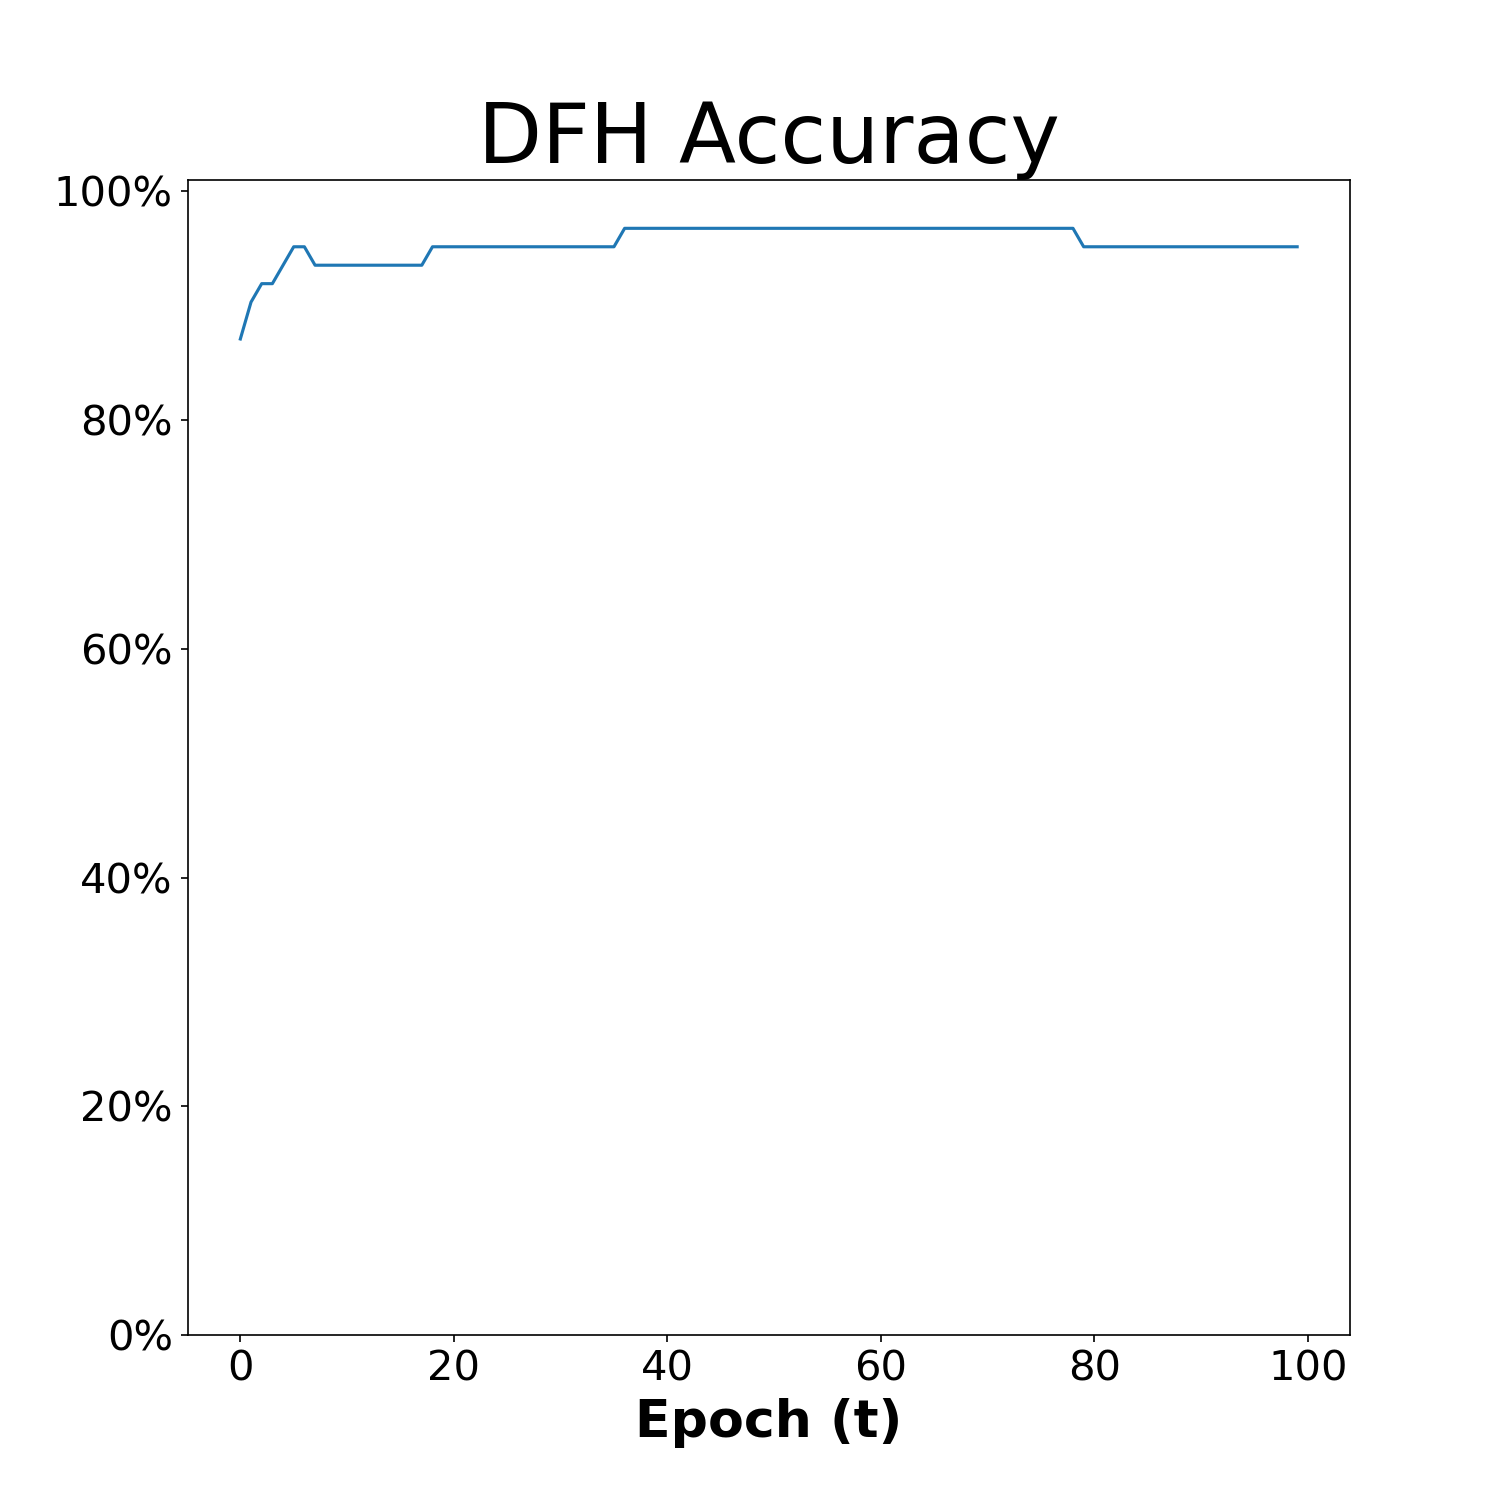
\includegraphics[width=\linewidth]{images/exper1/breast/DFH_0.01_acc.png}
    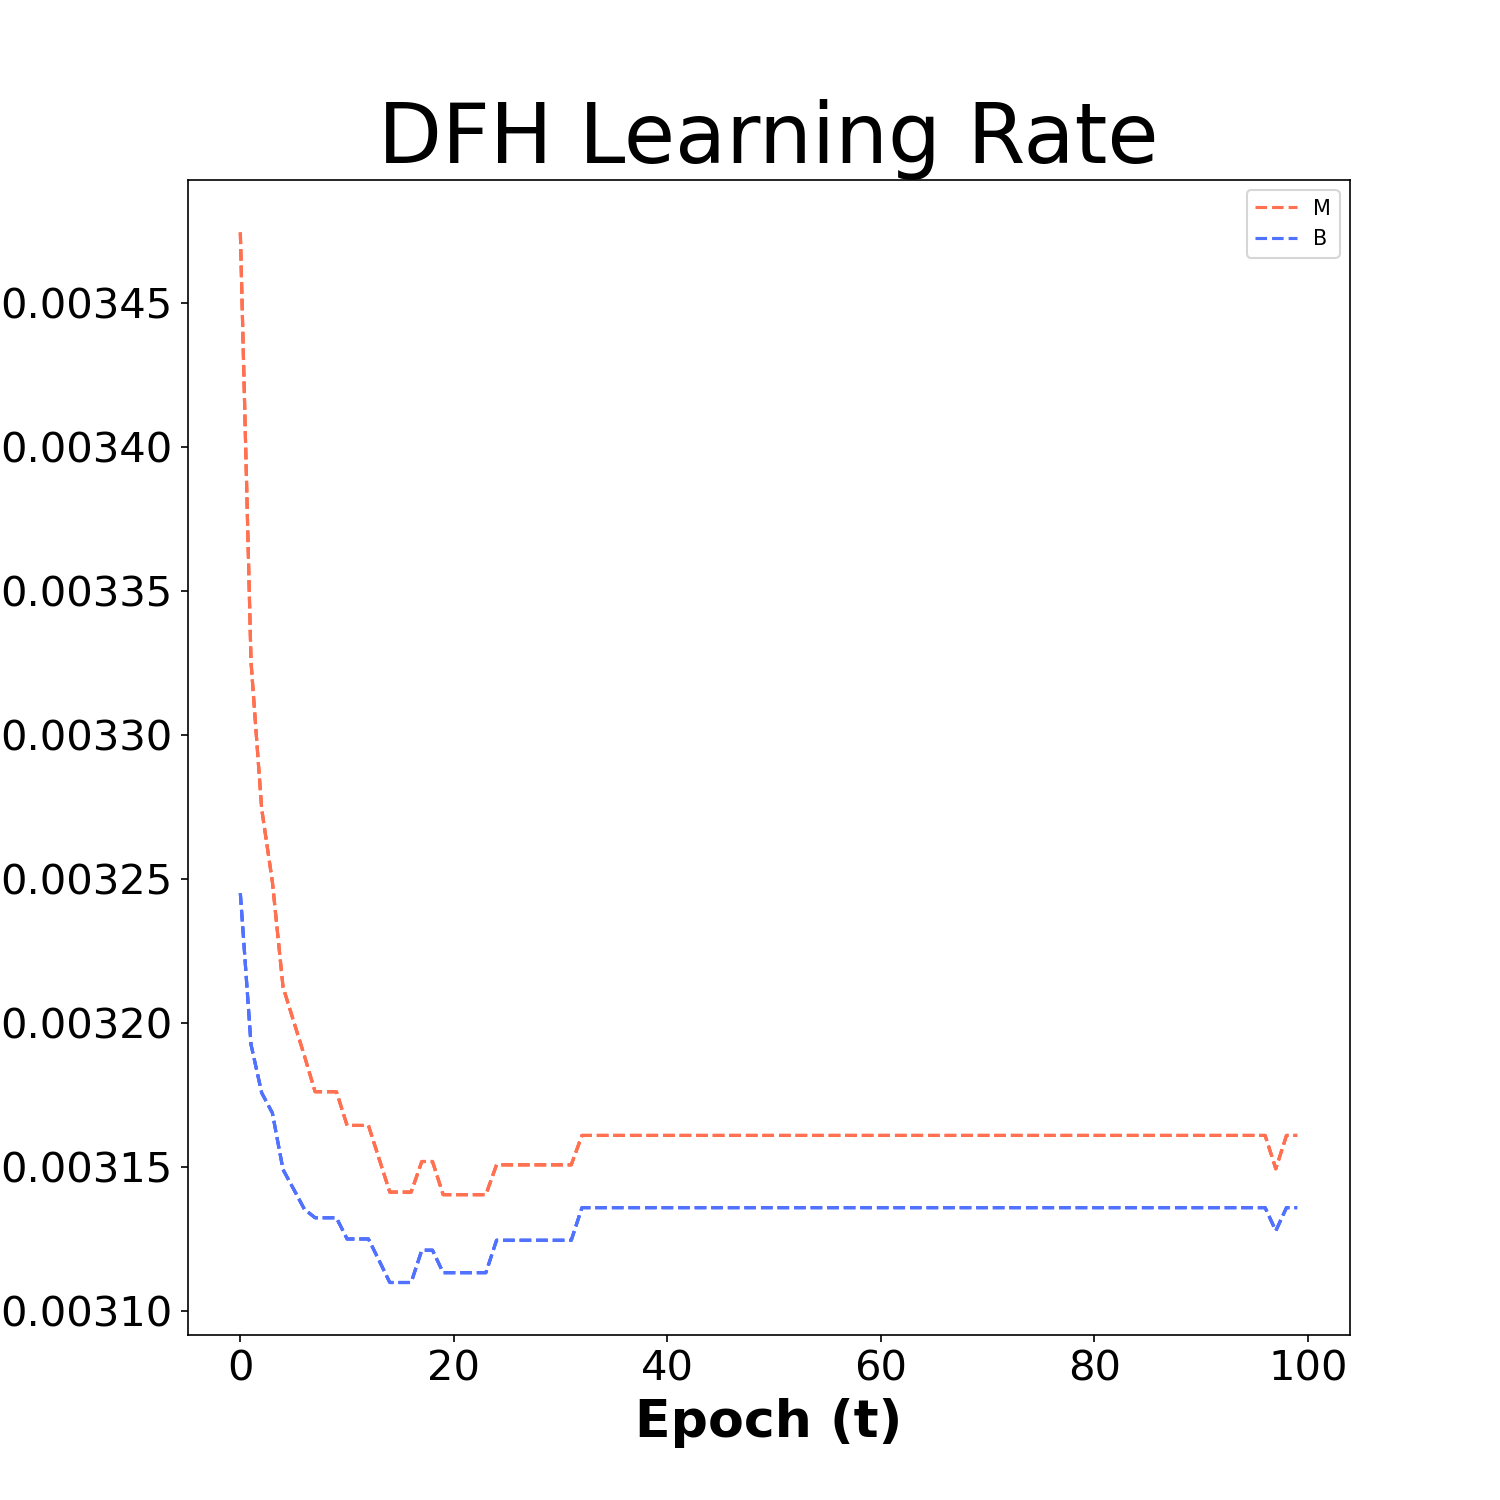
\includegraphics[width=\linewidth]{images/exper1/breast/DFH_0.01_lr.png}
  \caption{$\epsilon(0)=0.01$}
\end{subfigure}\hfil % <-- added
\begin{subfigure}{0.3\textwidth}
  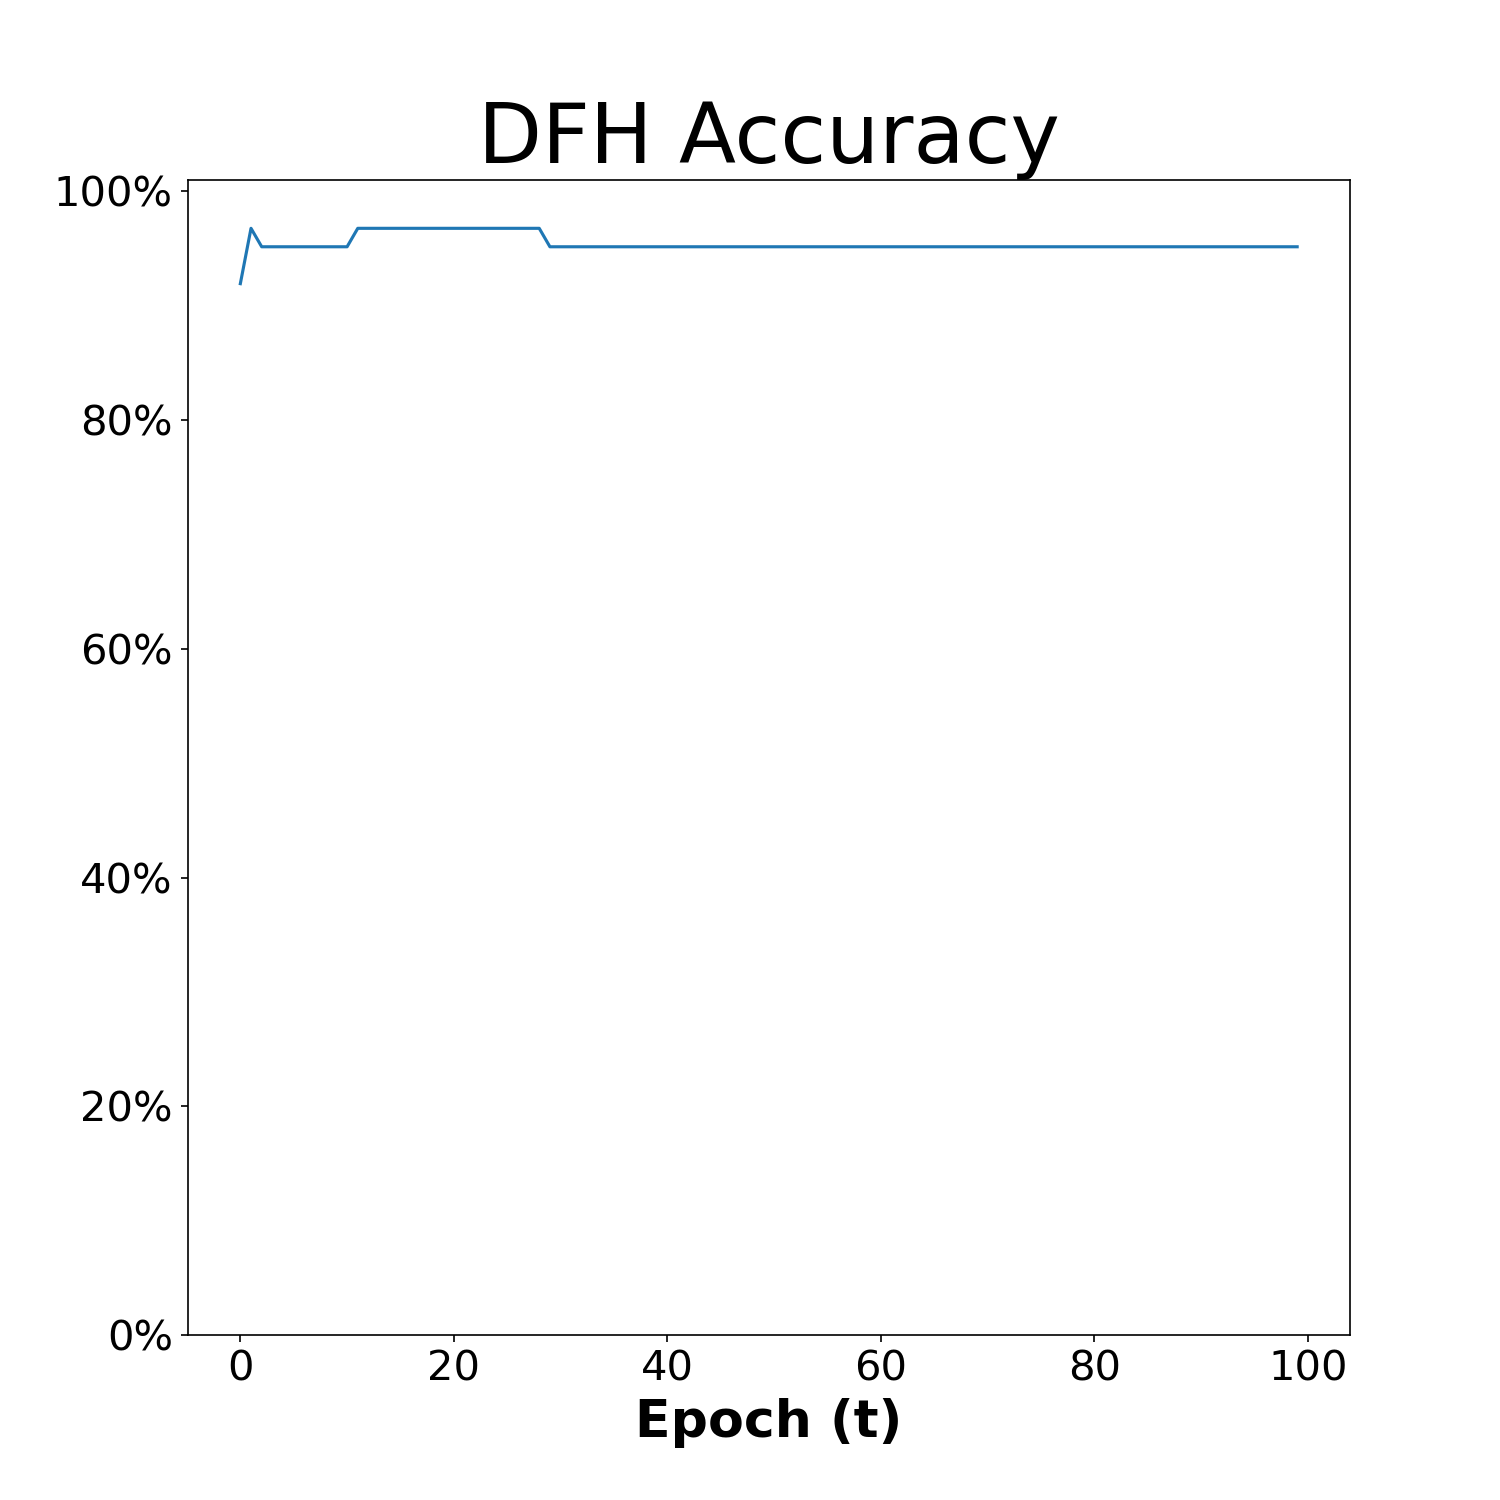
\includegraphics[width=\linewidth]{images/exper1/breast/DFH_0.03_acc.png}
  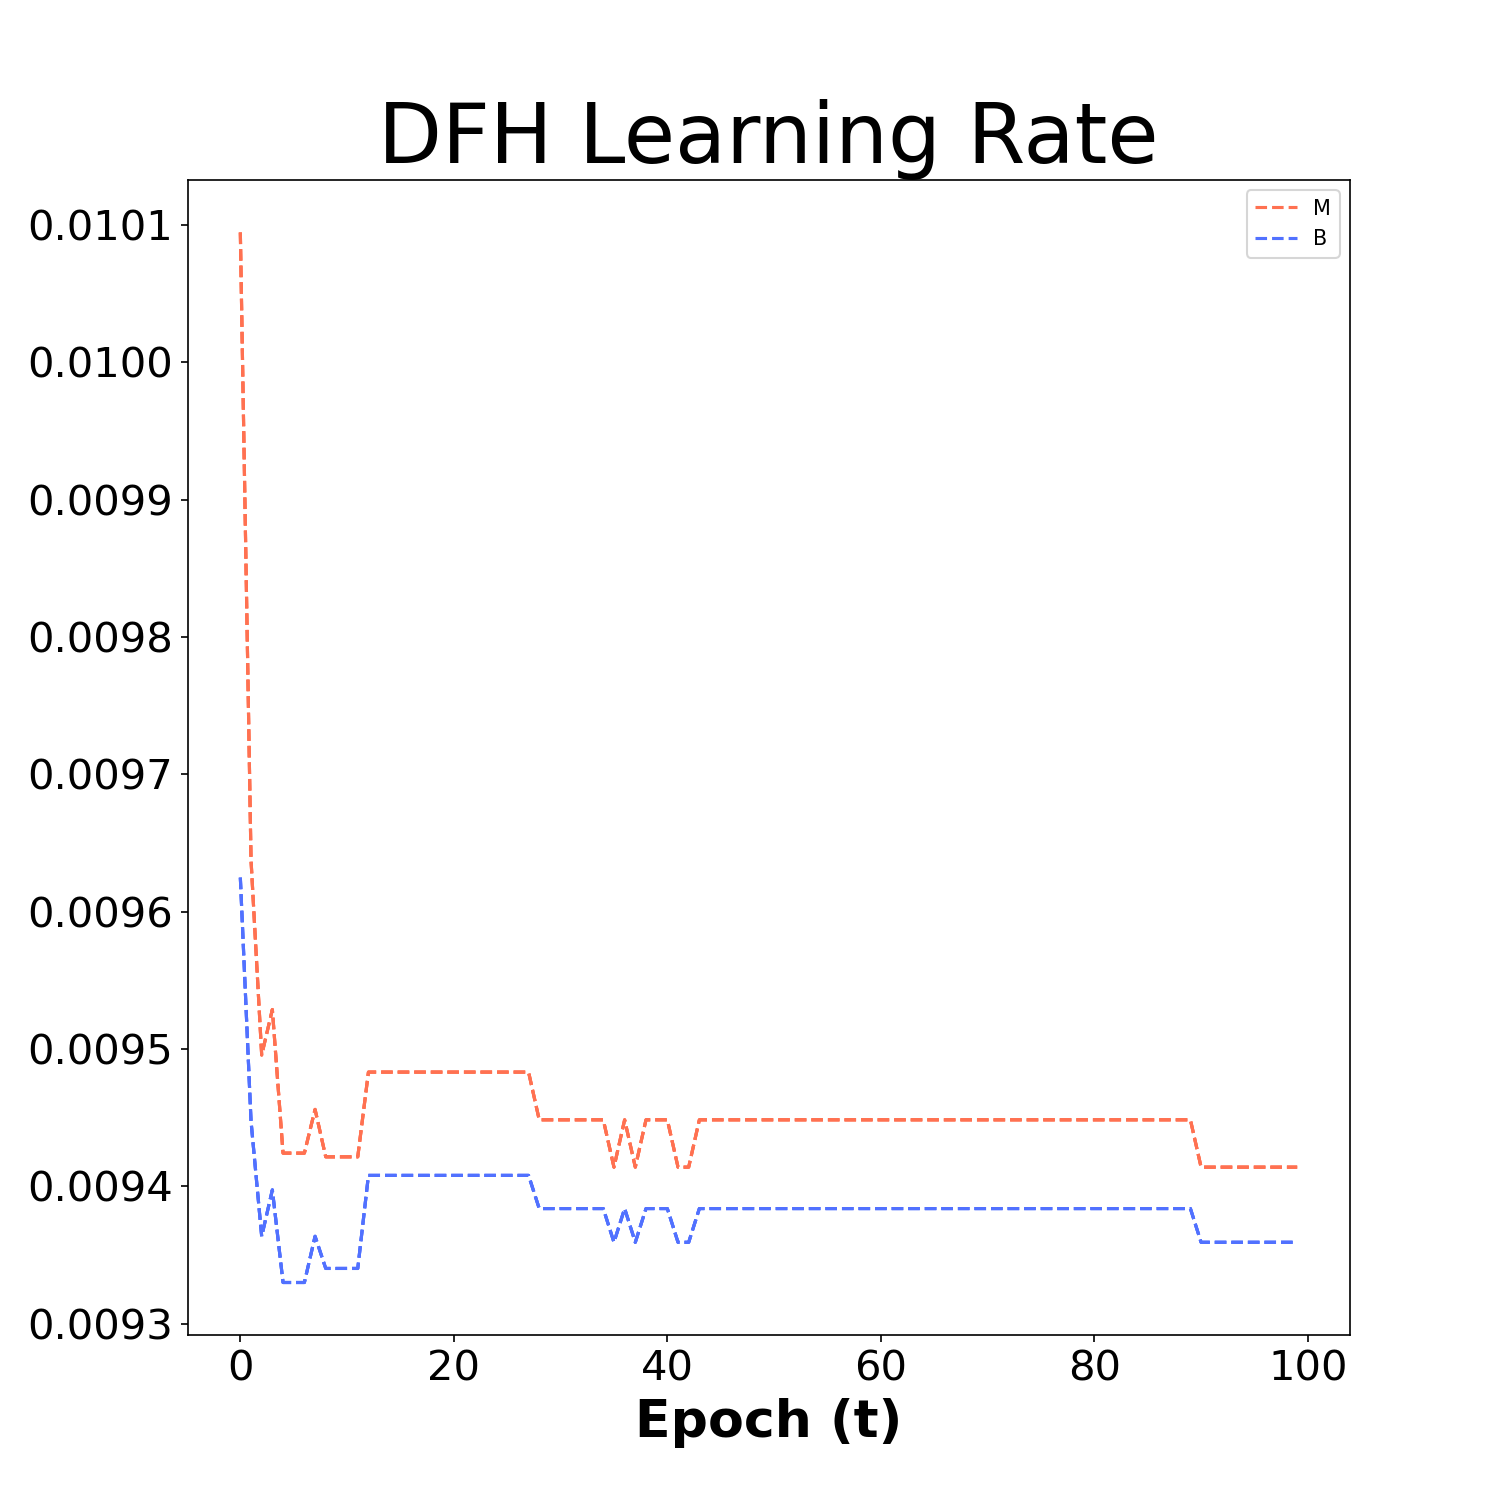
\includegraphics[width=\linewidth]{images/exper1/breast/DFH_0.03_lr.png}
  \caption{$\epsilon(0)=0.03$}
\end{subfigure}\hfil % <-- added
\begin{subfigure}{0.3\textwidth}
  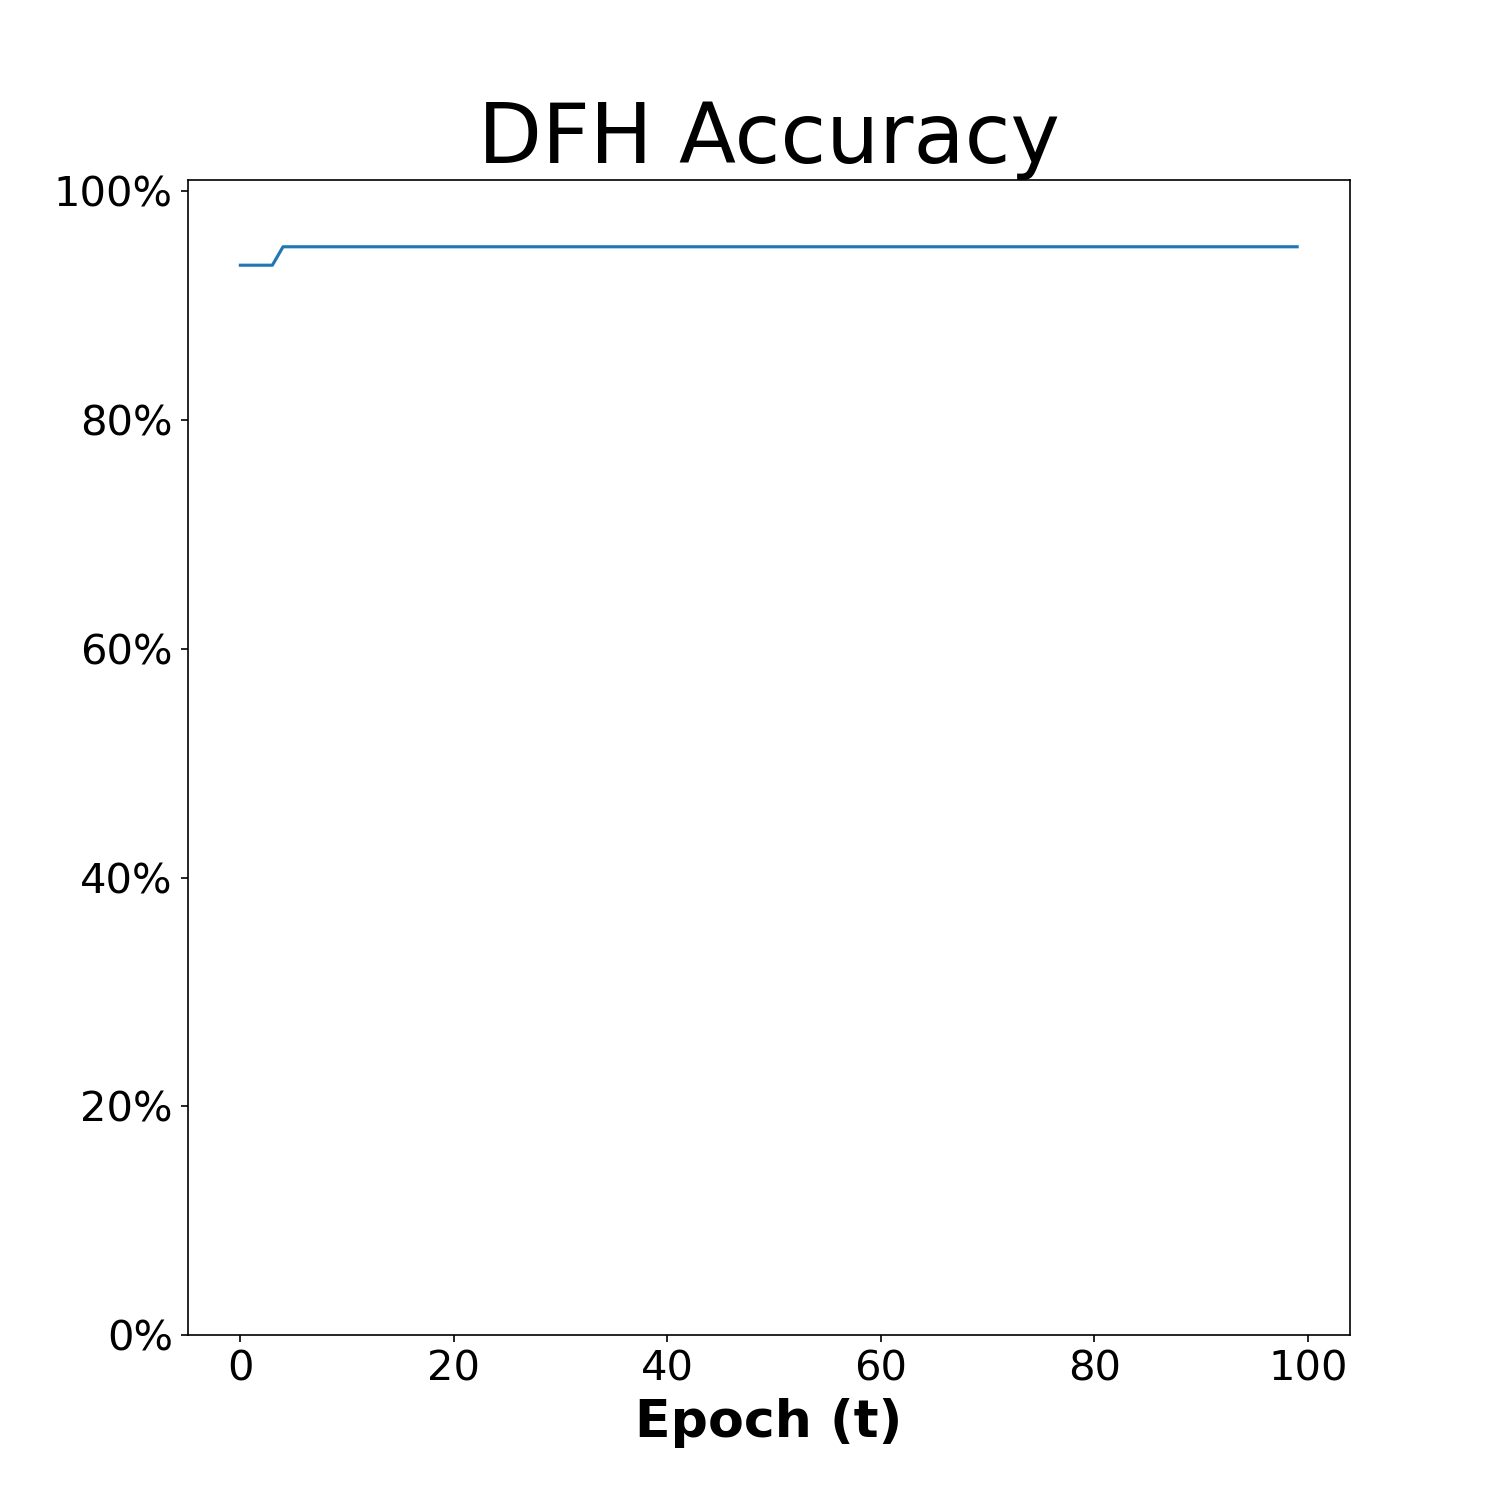
\includegraphics[width=\linewidth]{images/exper1/breast/DFH_0.1_acc.png}
  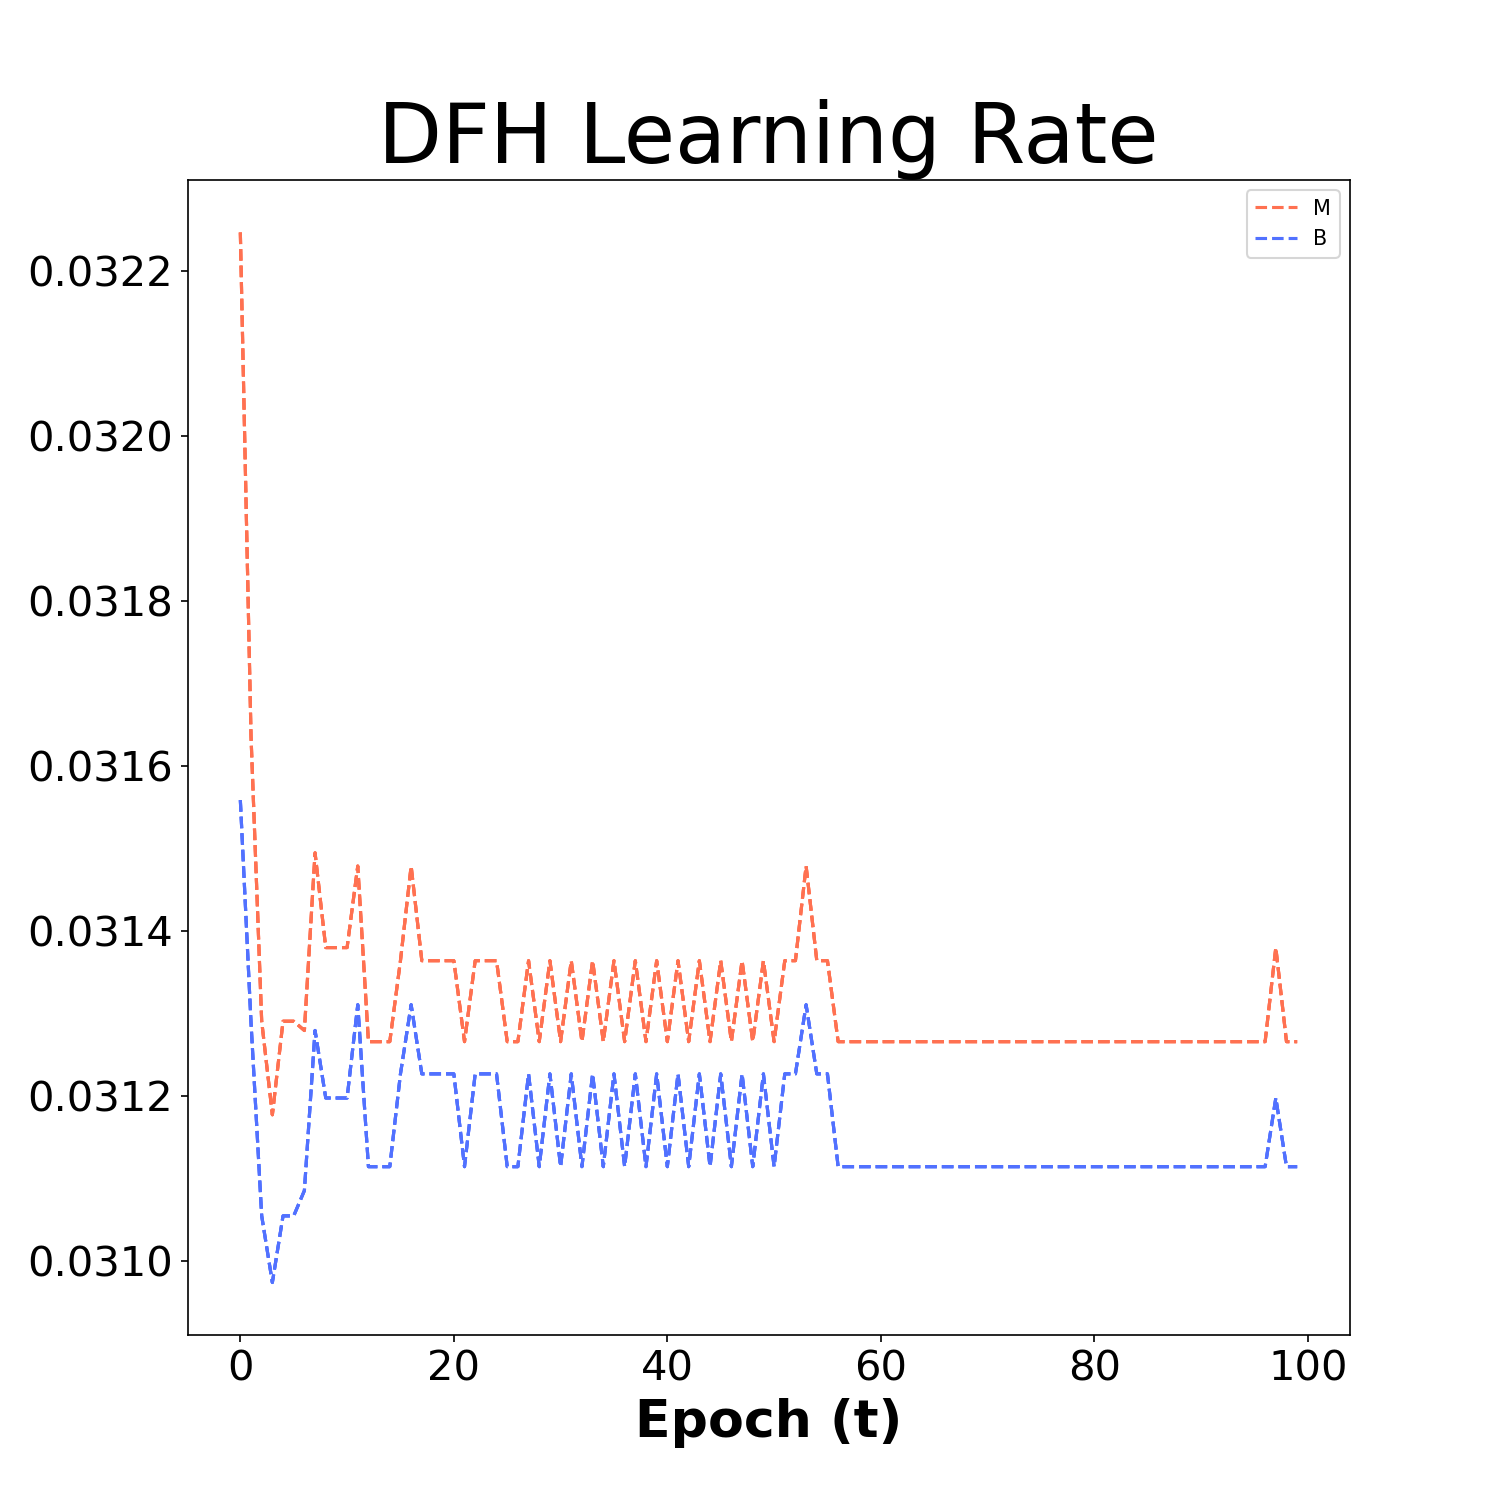
\includegraphics[width=\linewidth]{images/exper1/breast/DFH_0.1_lr.png}
  \caption{$\epsilon(0)=0.1$}
\end{subfigure}

\caption{\textit{Breast Cancer Wisconsin} dataset accuracy score and learning rate results under DFH model using balanced dataset.}
\end{figure}

\begin{figure}[H]
    \centering % <-- added
\begin{subfigure}{0.3\textwidth}
  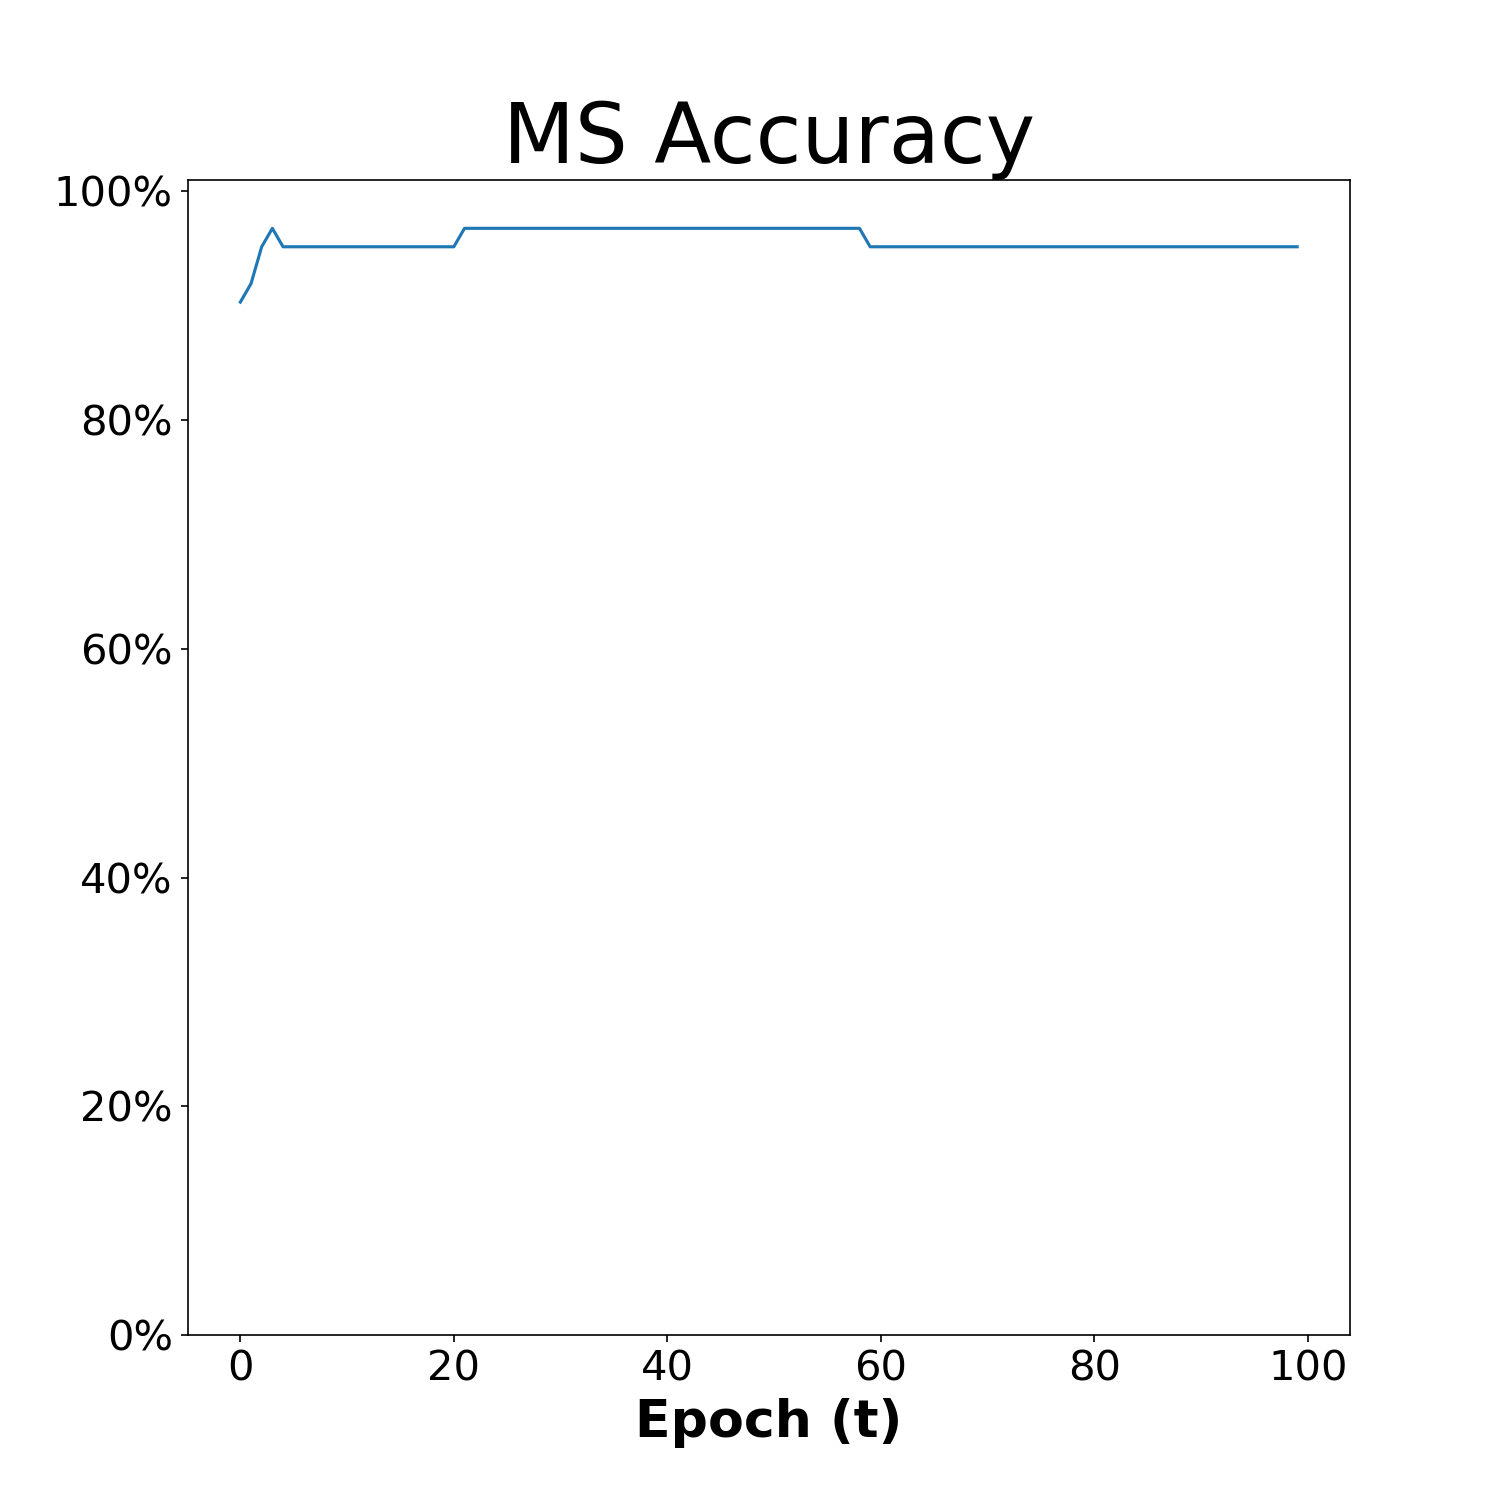
\includegraphics[width=\linewidth]{images/exper1/breast/MS_0.01_acc.png}
    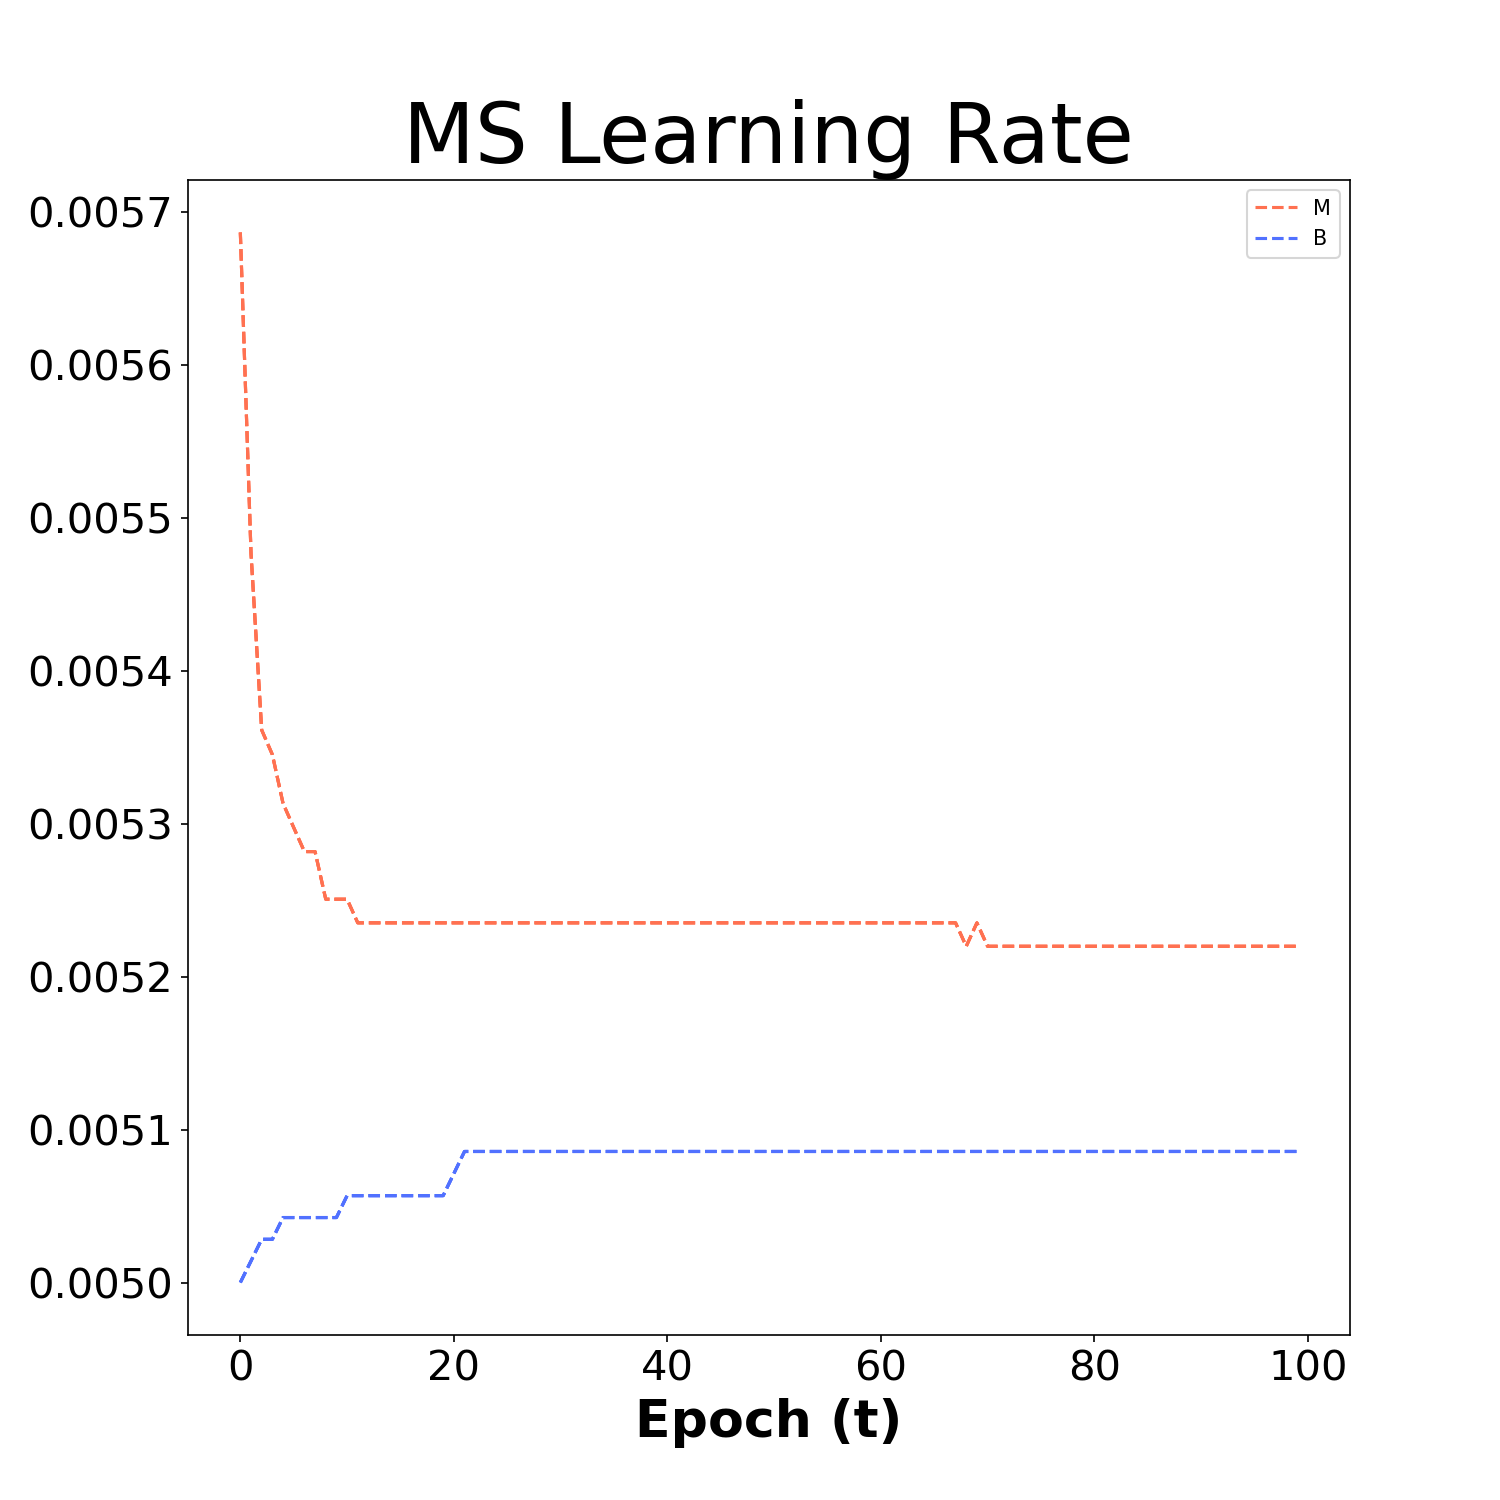
\includegraphics[width=\linewidth]{images/exper1/breast/MS_0.01_lr.png}
  \caption{$\epsilon(0)=0.01$}
\end{subfigure}\hfil % <-- added
\begin{subfigure}{0.3\textwidth}
  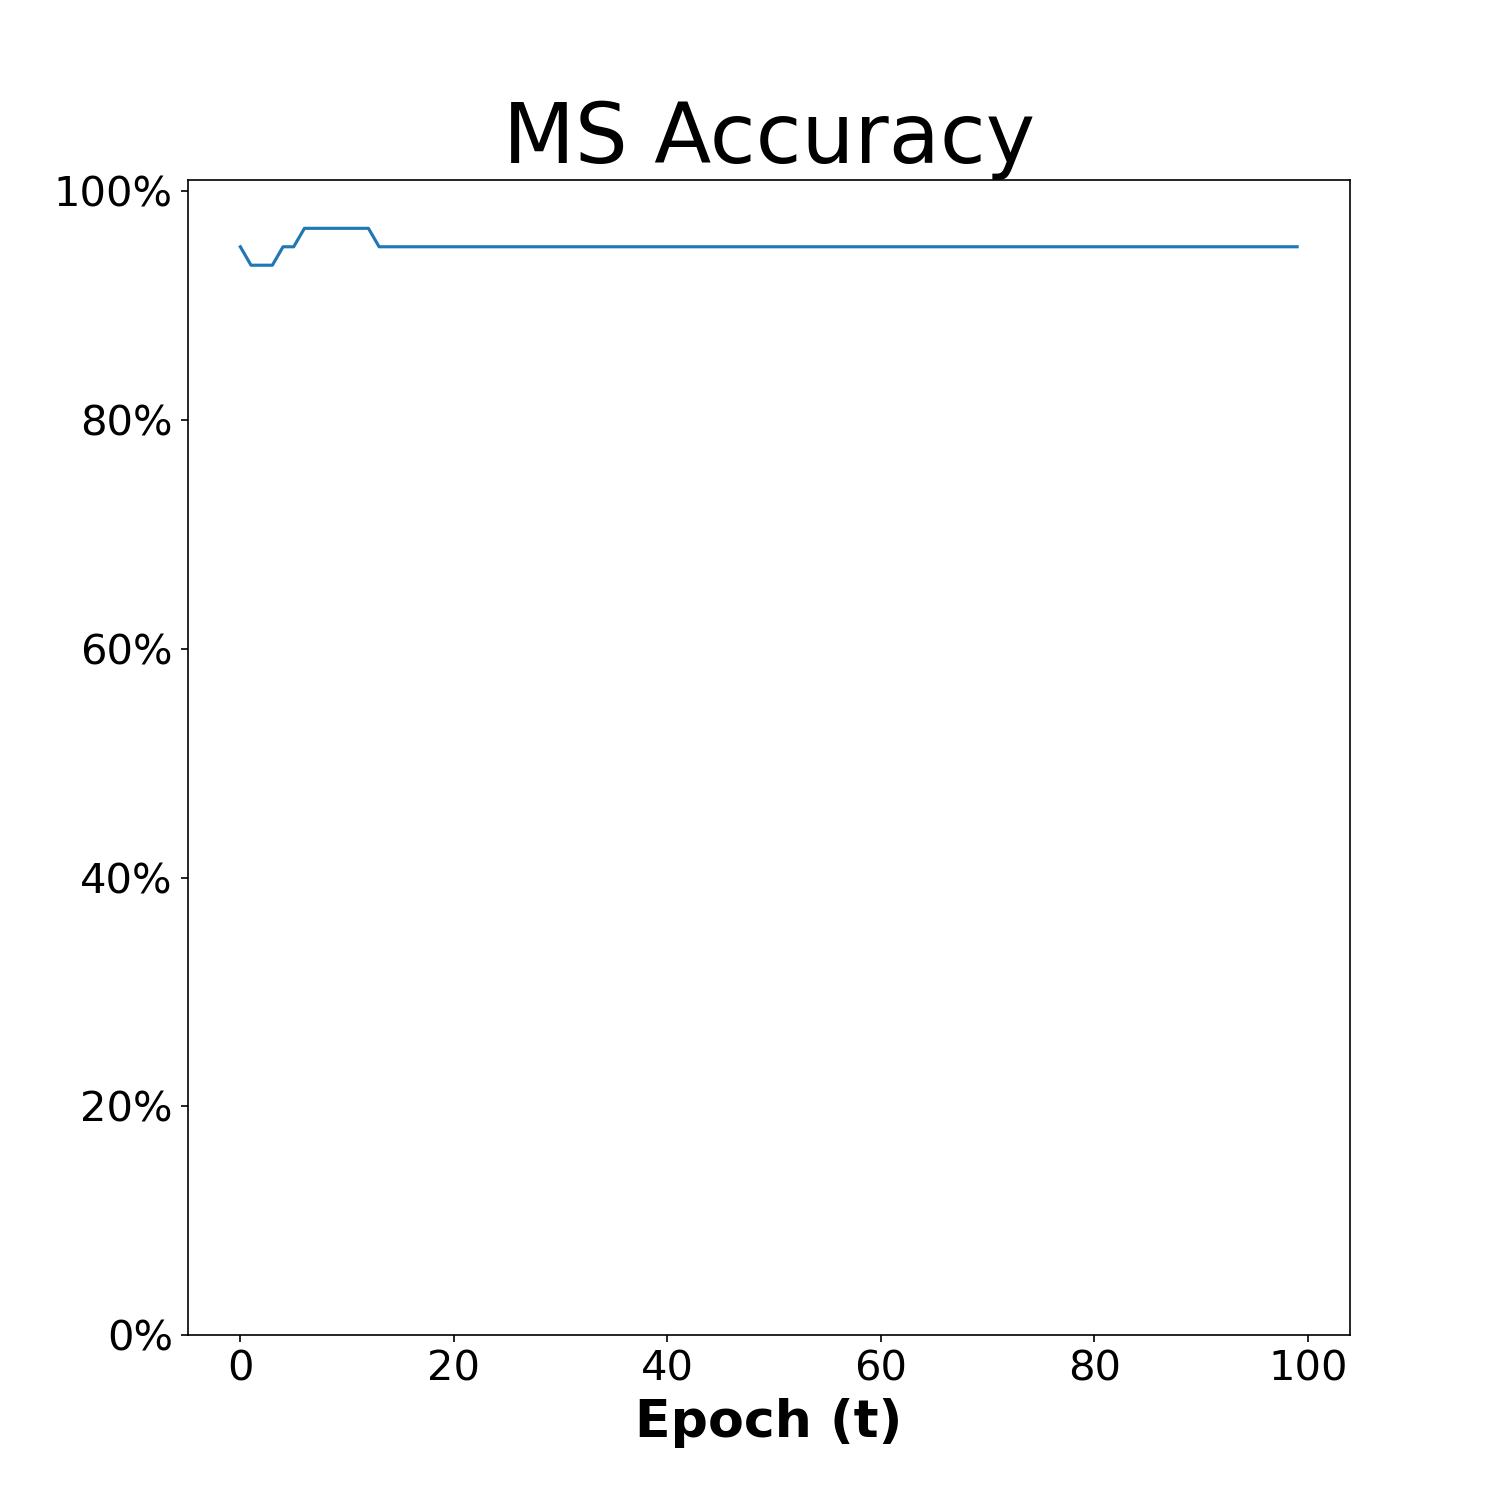
\includegraphics[width=\linewidth]{images/exper1/breast/MS_0.03_acc.png}
  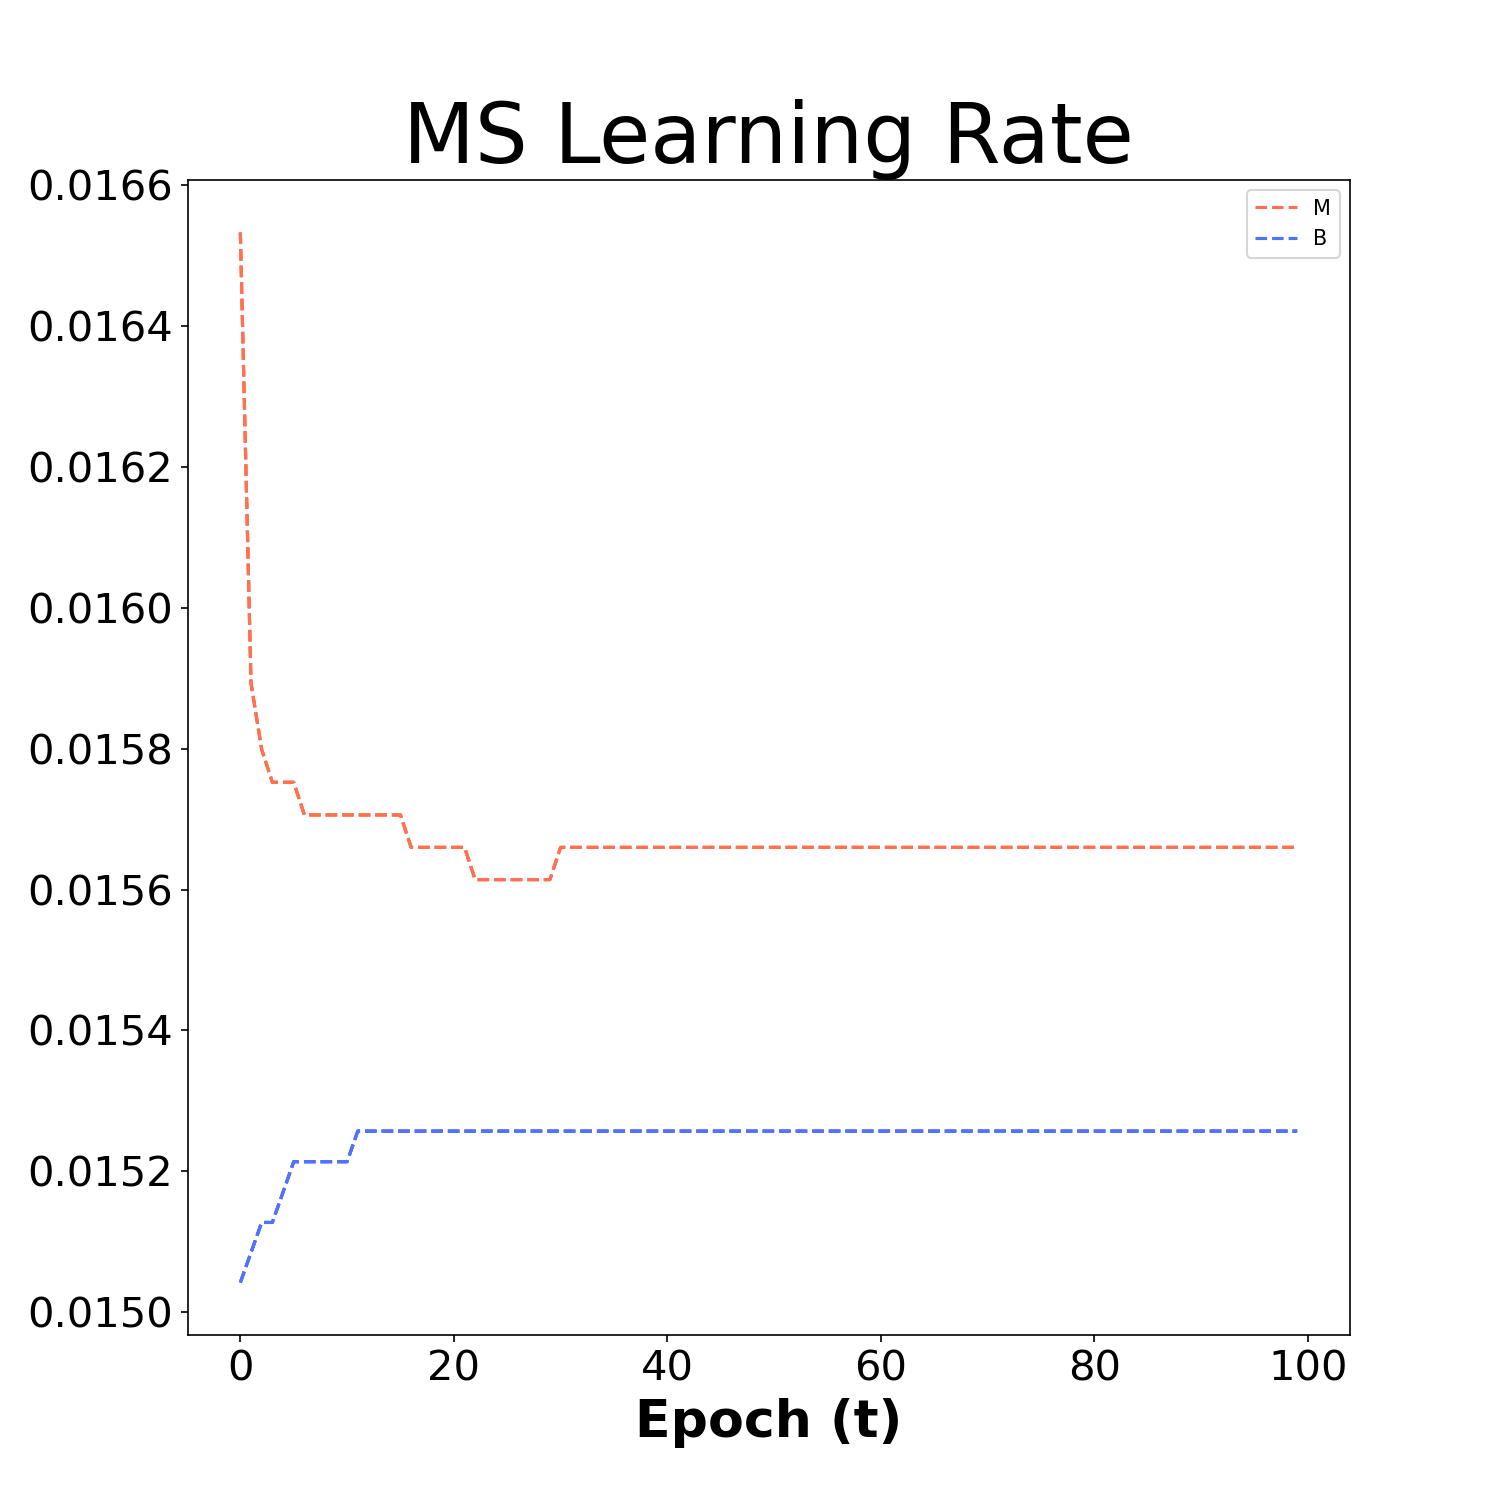
\includegraphics[width=\linewidth]{images/exper1/breast/MS_0.03_lr.png}
  \caption{$\epsilon(0)=0.03$}
\end{subfigure}\hfil % <-- added
\begin{subfigure}{0.3\textwidth}
  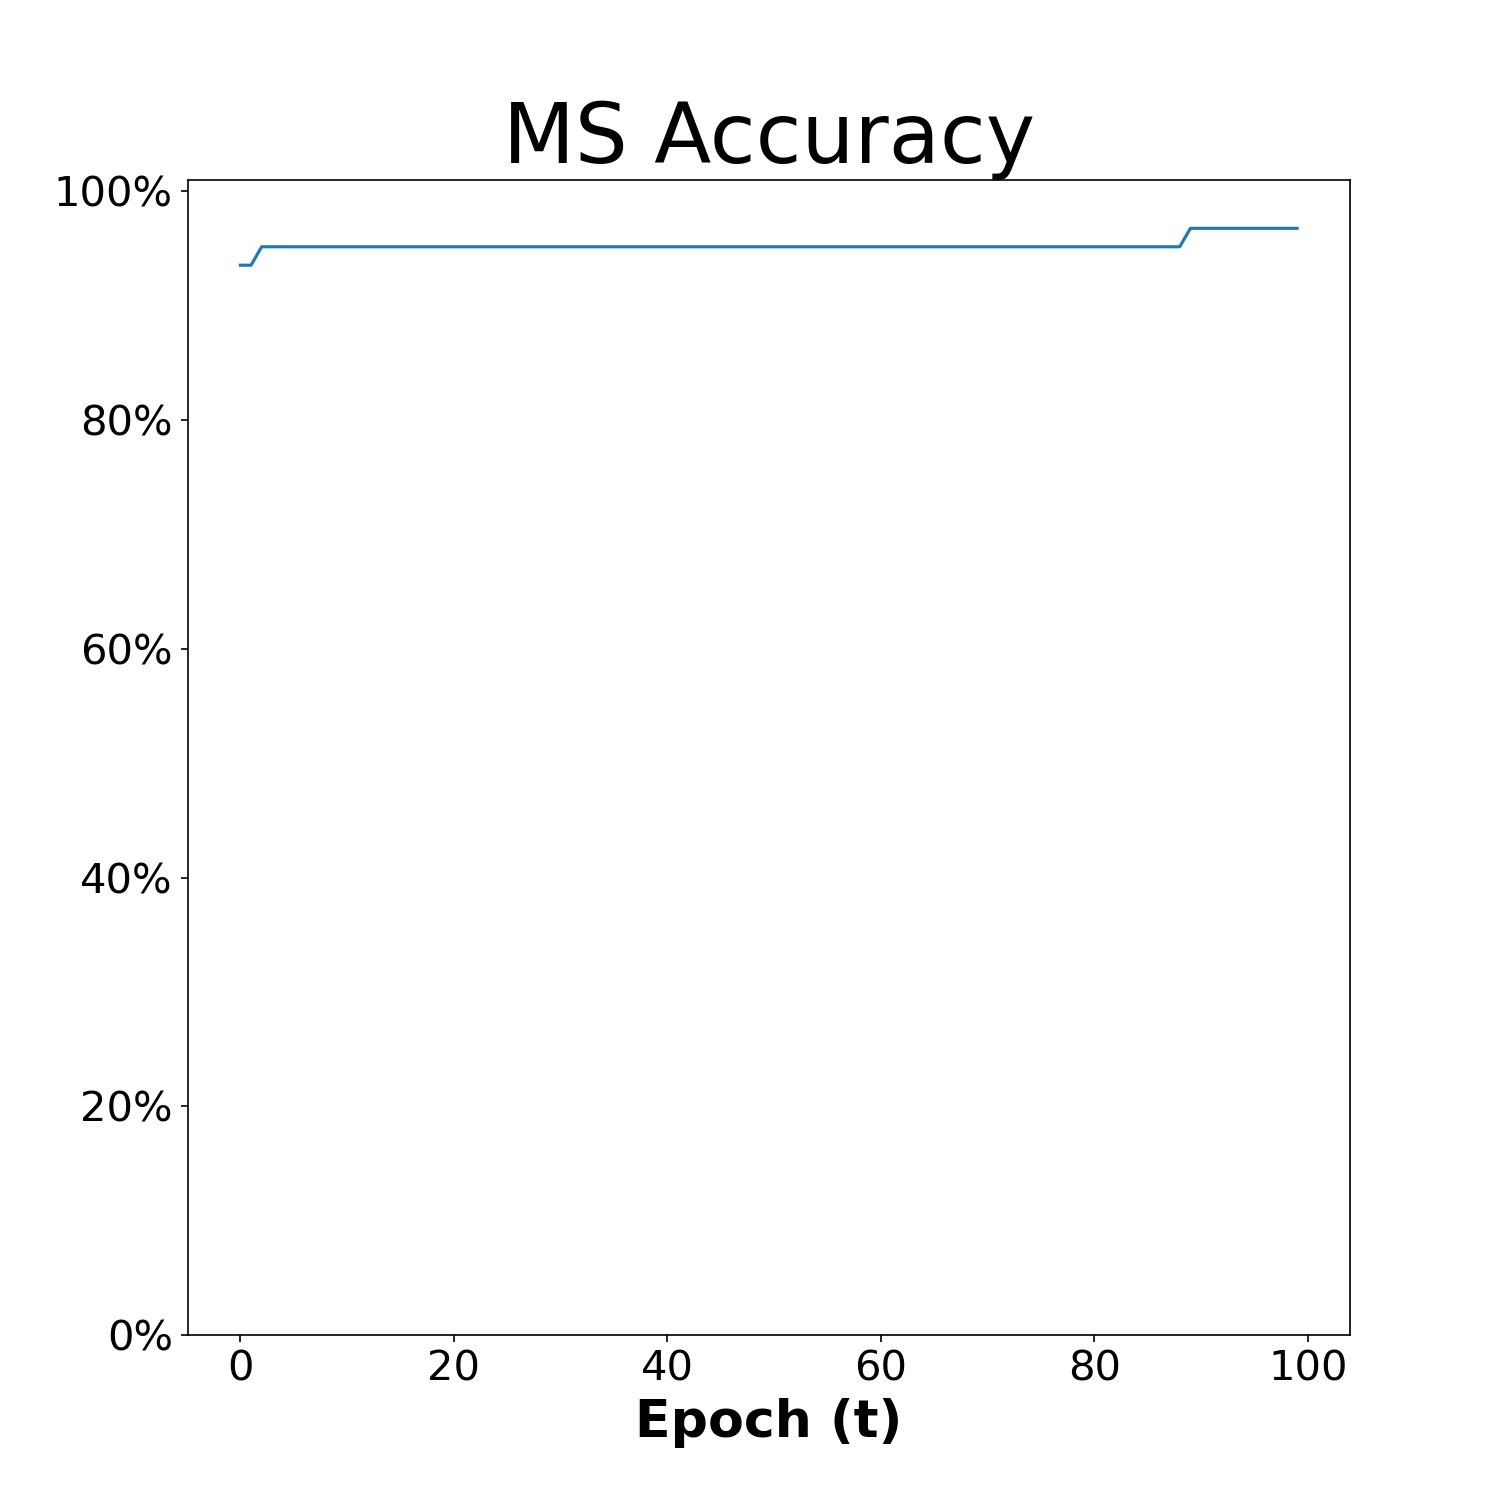
\includegraphics[width=\linewidth]{images/exper1/breast/MS_0.1_acc.png}
  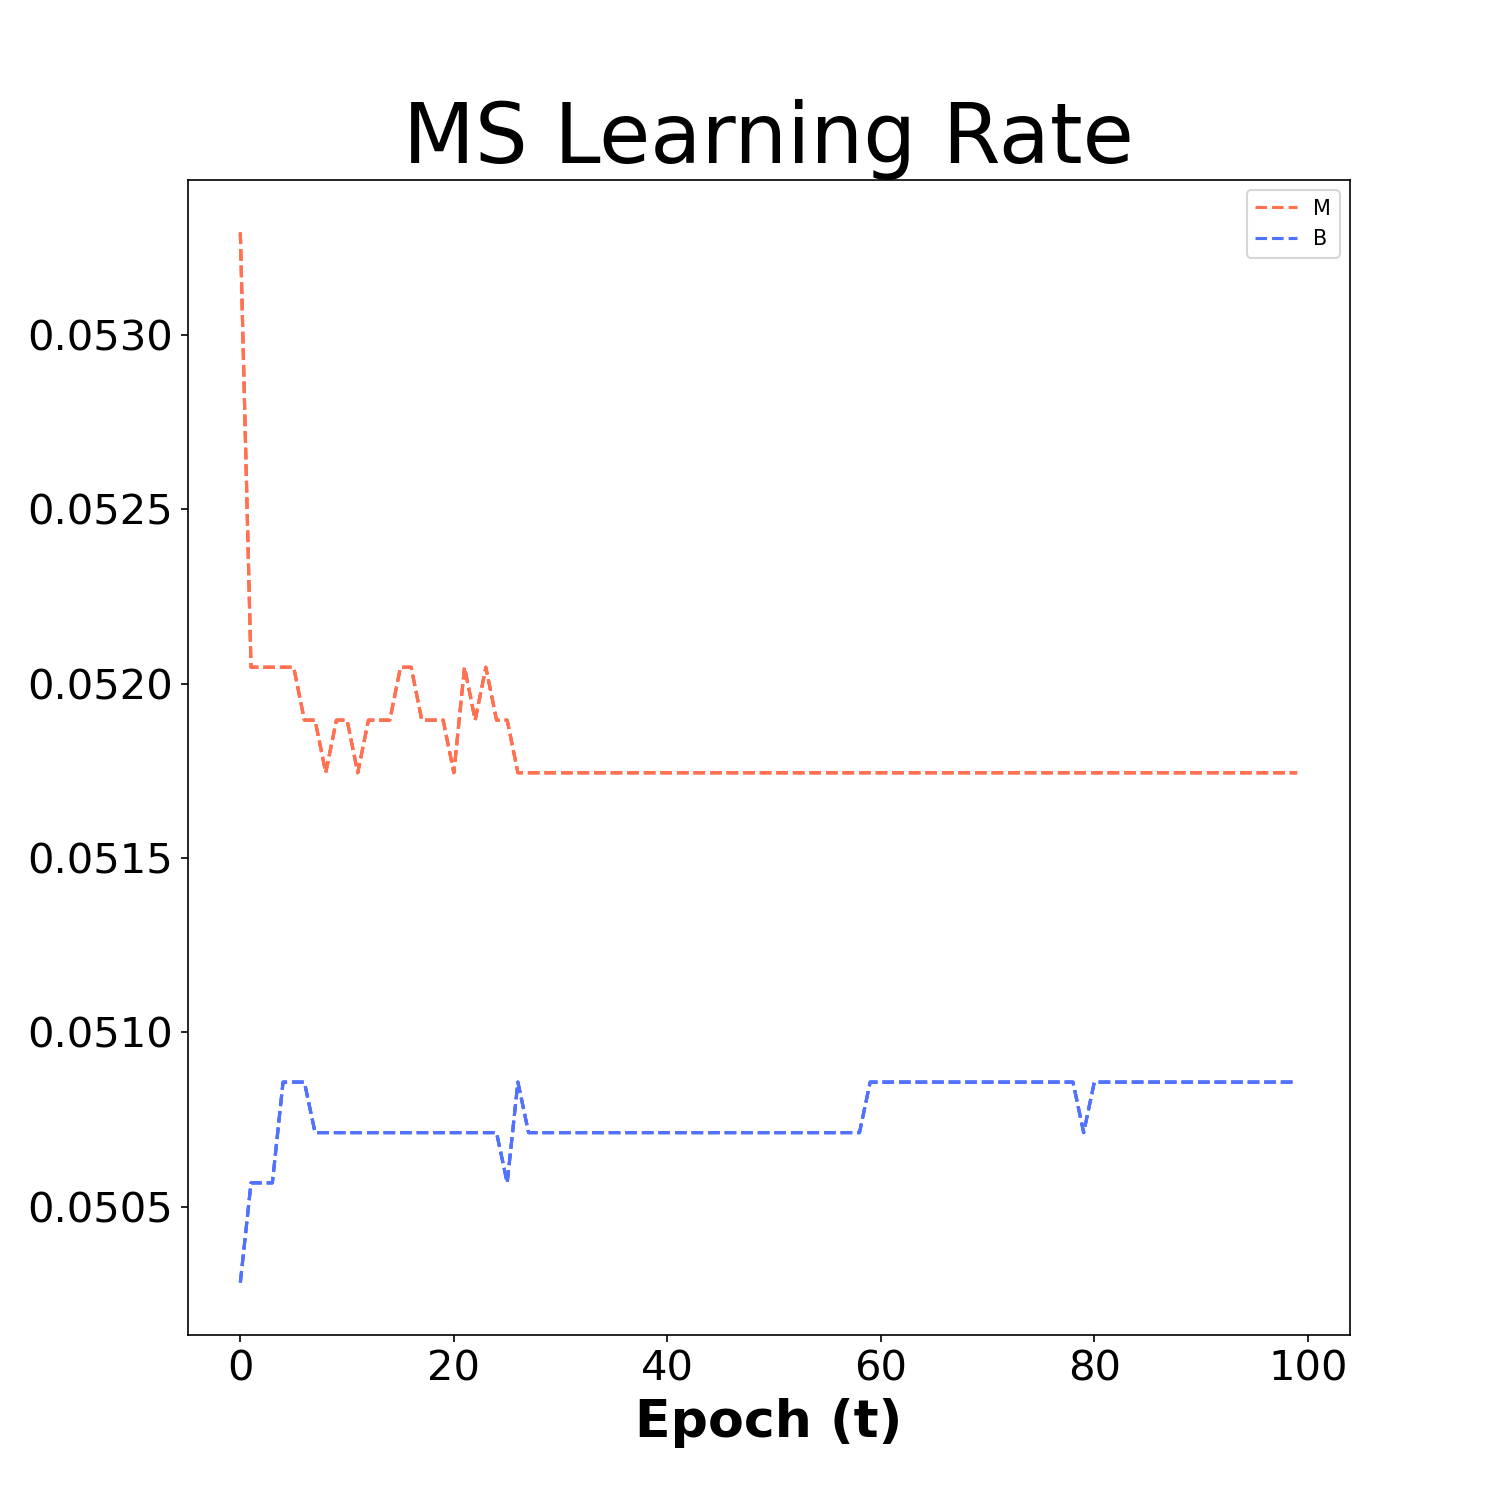
\includegraphics[width=\linewidth]{images/exper1/breast/MS_0.1_lr.png}
  \caption{$\epsilon(0)=0.1$}
\end{subfigure}

\caption{\textit{Breast Cancer Wisconsin} dataset accuracy score and learning rate results under MS model using balanced dataset.}
\end{figure}

\begin{figure}[H]
    \centering % <-- added
\begin{subfigure}{0.3\textwidth}
  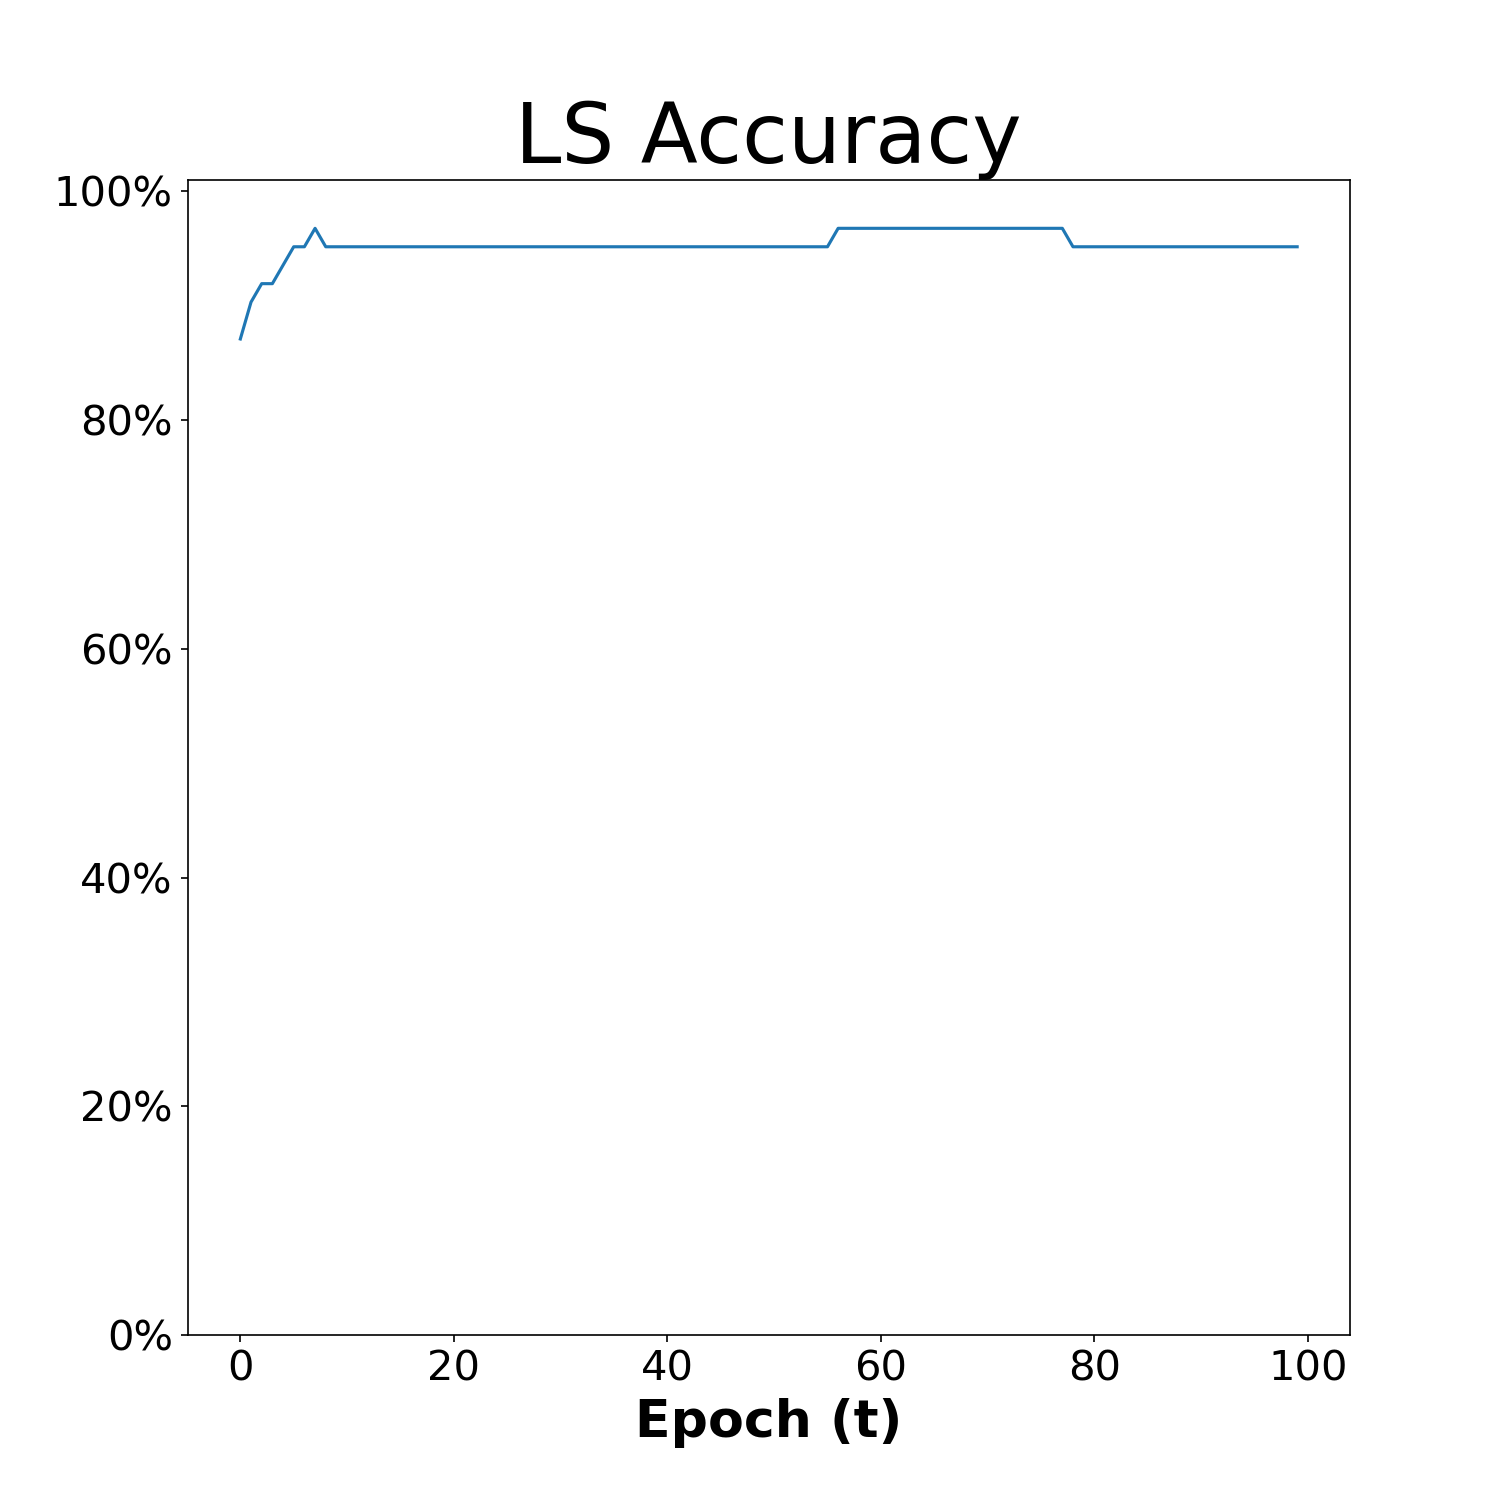
\includegraphics[width=\linewidth]{images/exper1/breast/LS_0.01_acc.png}
    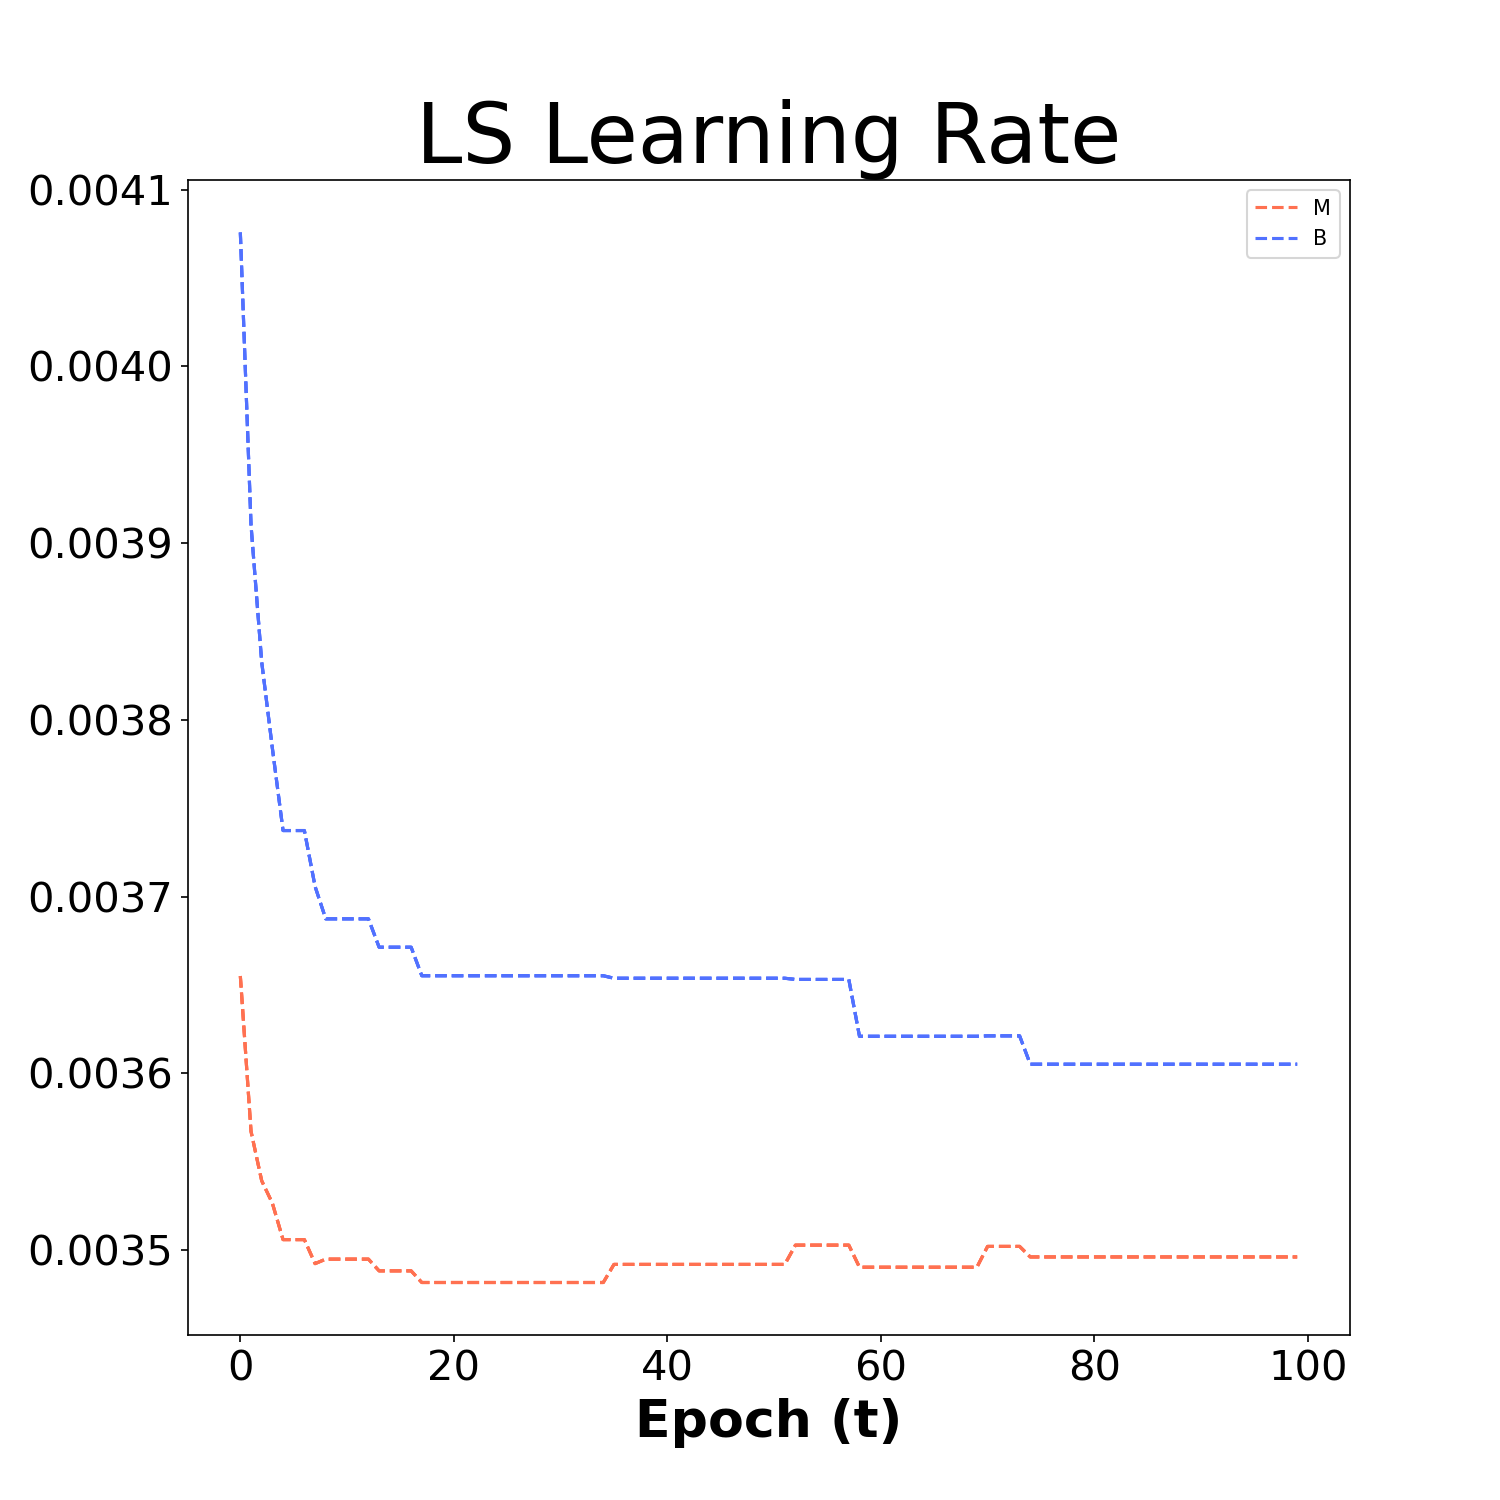
\includegraphics[width=\linewidth]{images/exper1/breast/LS_0.01_lr.png}
  \caption{$\epsilon(0)=0.01$}
\end{subfigure}\hfil % <-- added
\begin{subfigure}{0.3\textwidth}
  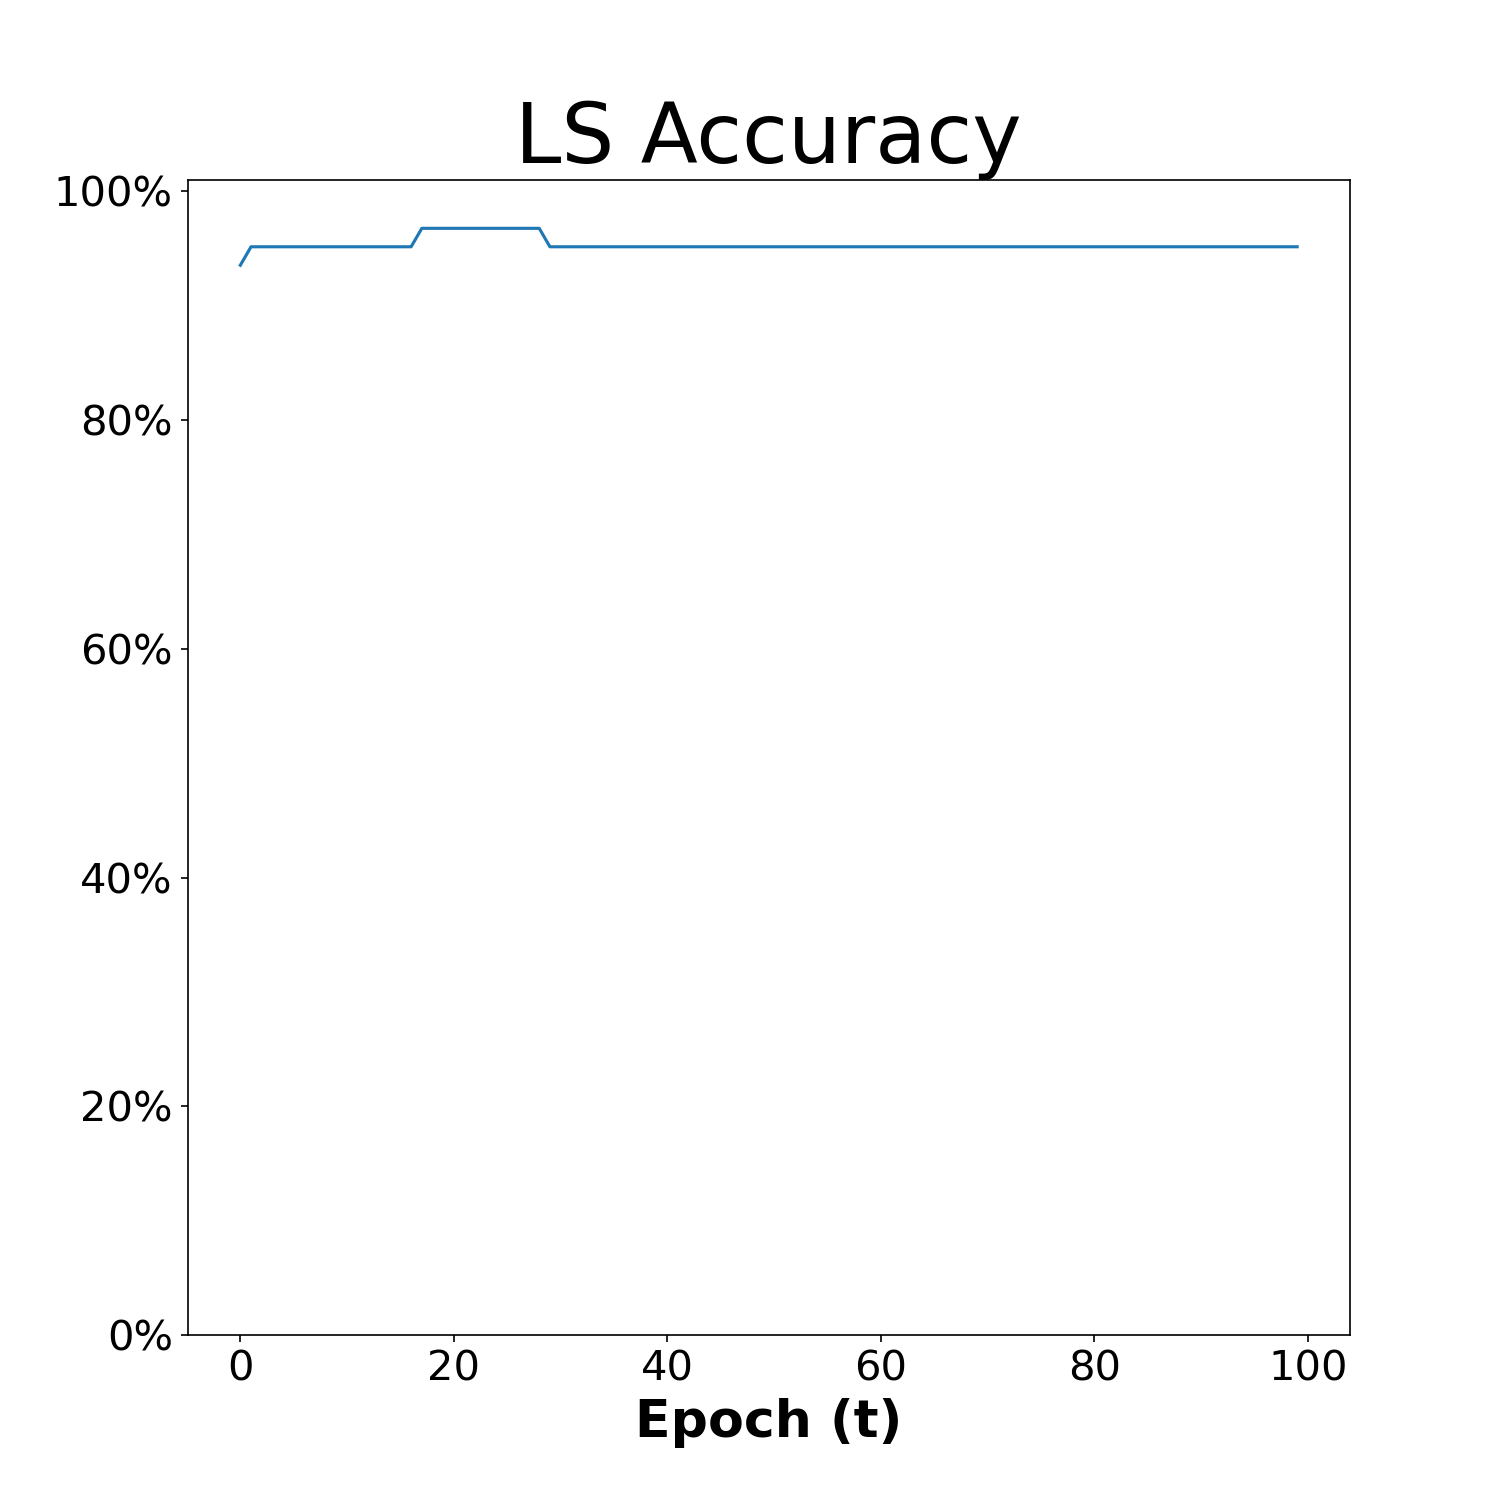
\includegraphics[width=\linewidth]{images/exper1/breast/LS_0.03_acc.png}
  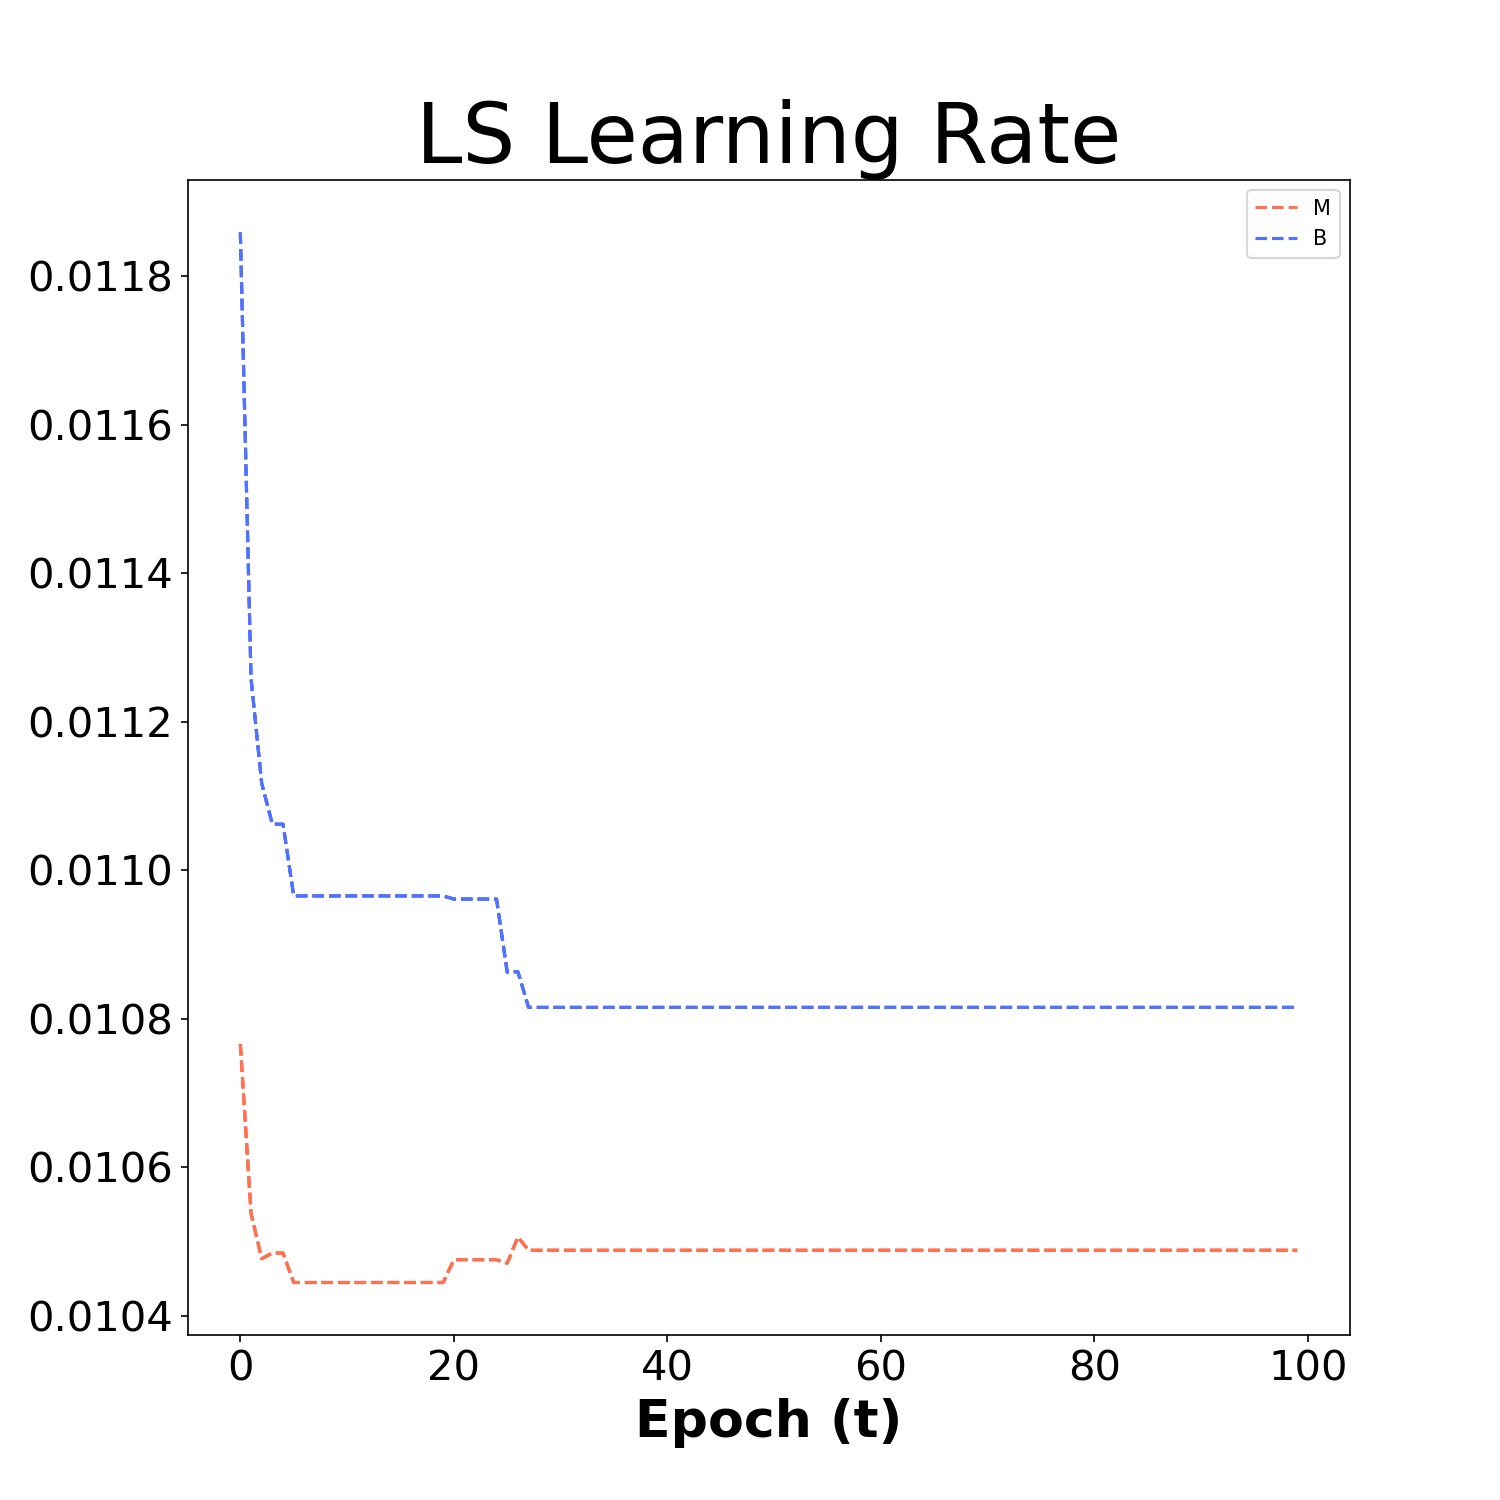
\includegraphics[width=\linewidth]{images/exper1/breast/LS_0.03_lr.png}
  \caption{$\epsilon(0)=0.03$}
\end{subfigure}\hfil % <-- added
\begin{subfigure}{0.3\textwidth}
  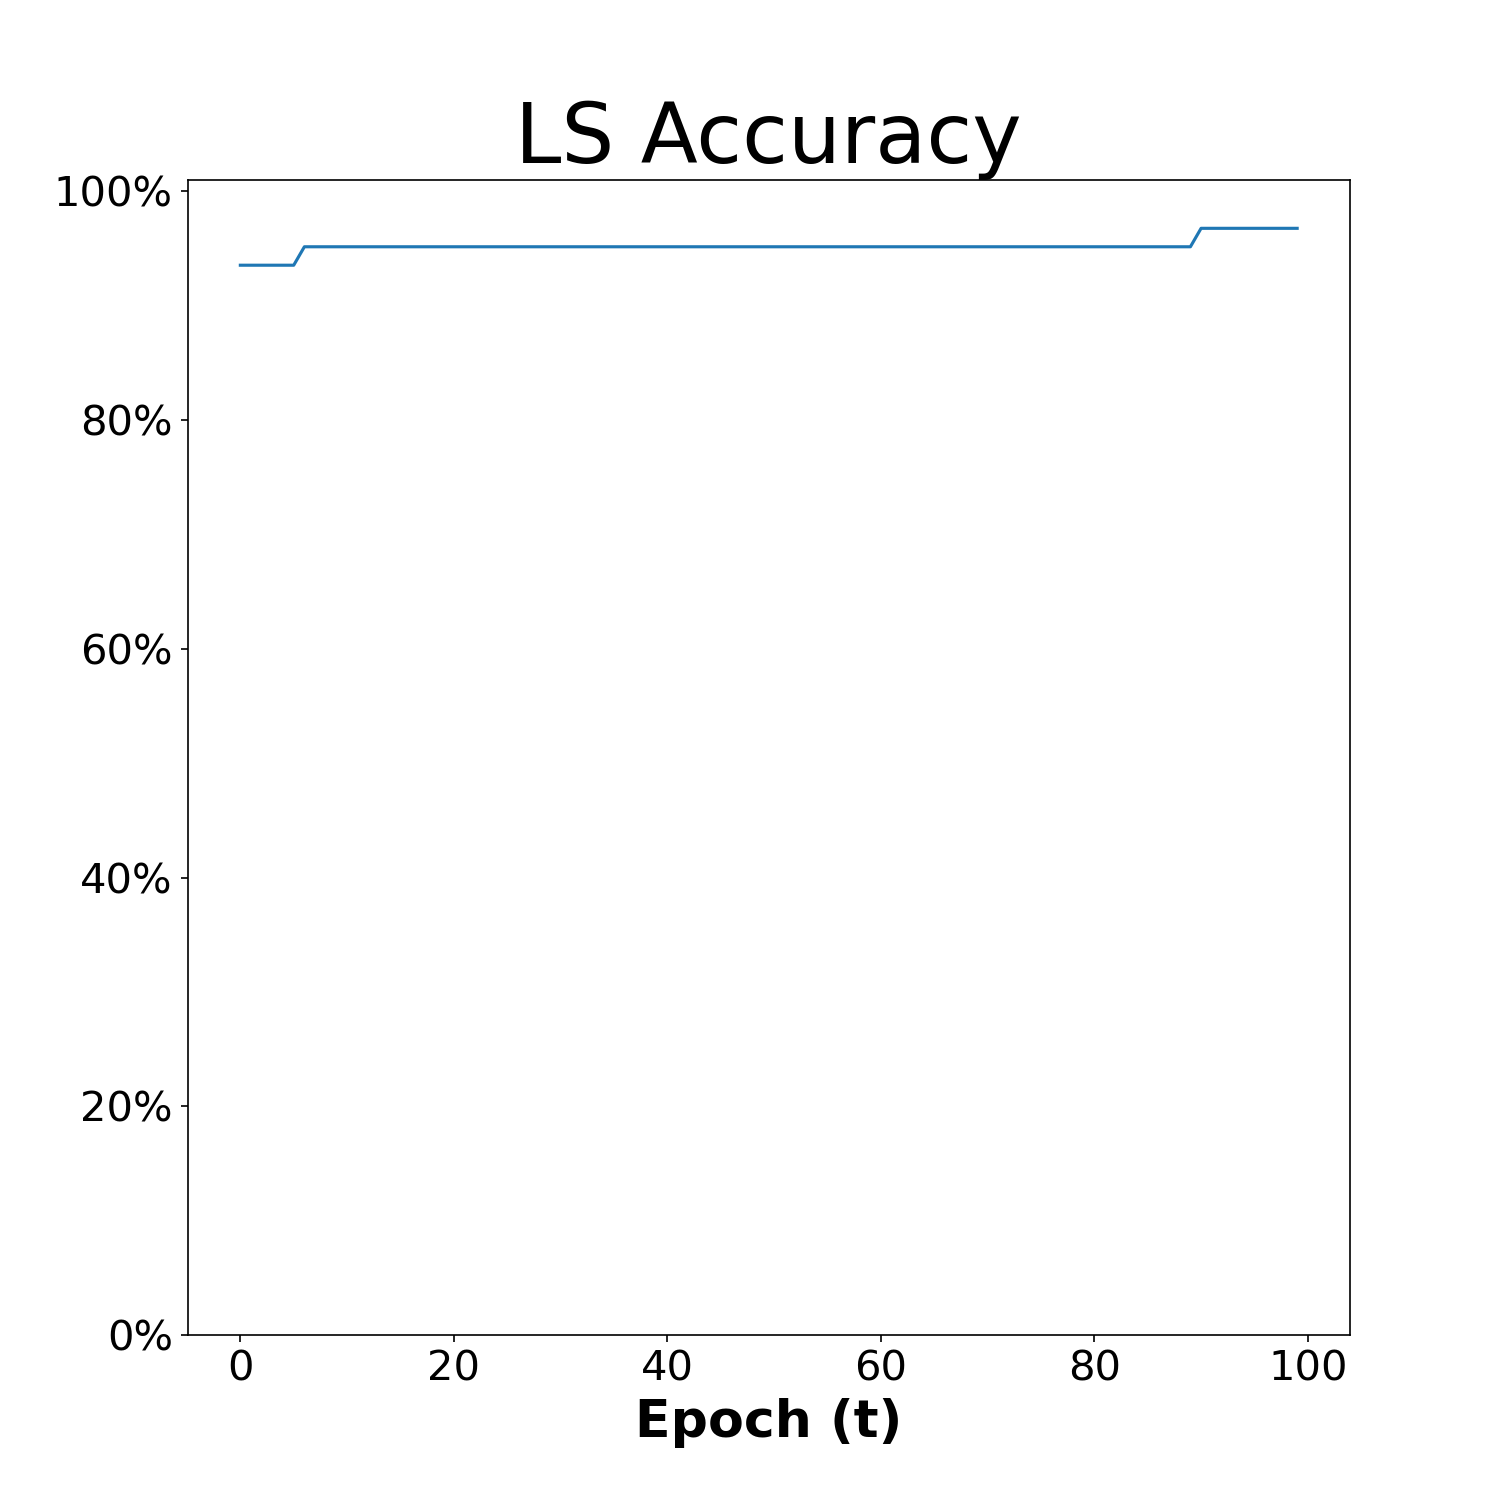
\includegraphics[width=\linewidth]{images/exper1/breast/LS_0.1_acc.png}
  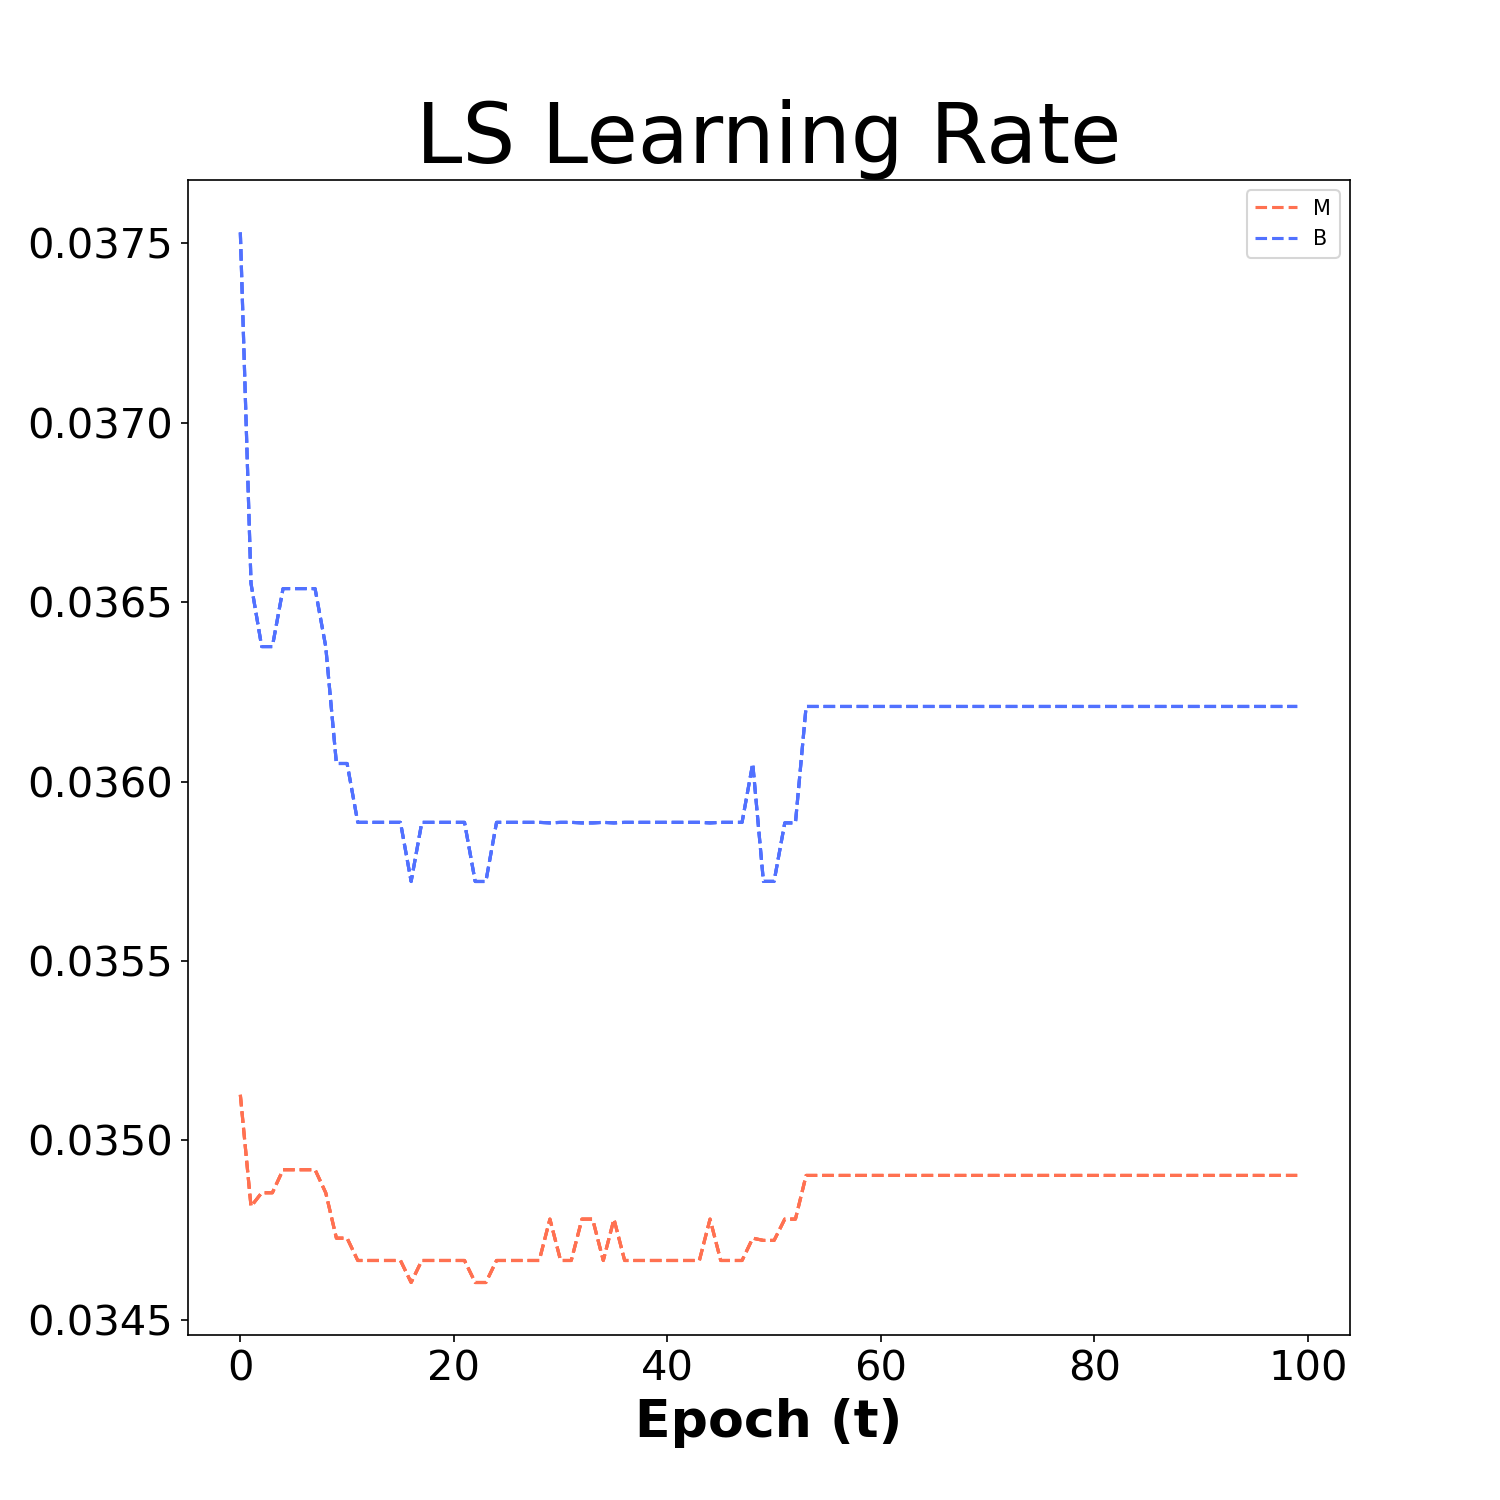
\includegraphics[width=\linewidth]{images/exper1/breast/LS_0.1_lr.png}
  \caption{$\epsilon(0)=0.1$}
\end{subfigure}

\caption{\textit{Breast Cancer Wisconsin} dataset accuracy score and learning rate results under LS model using balanced dataset.}
\end{figure}

\begin{figure}[H]
    \centering % <-- added
\begin{subfigure}{0.3\textwidth}
  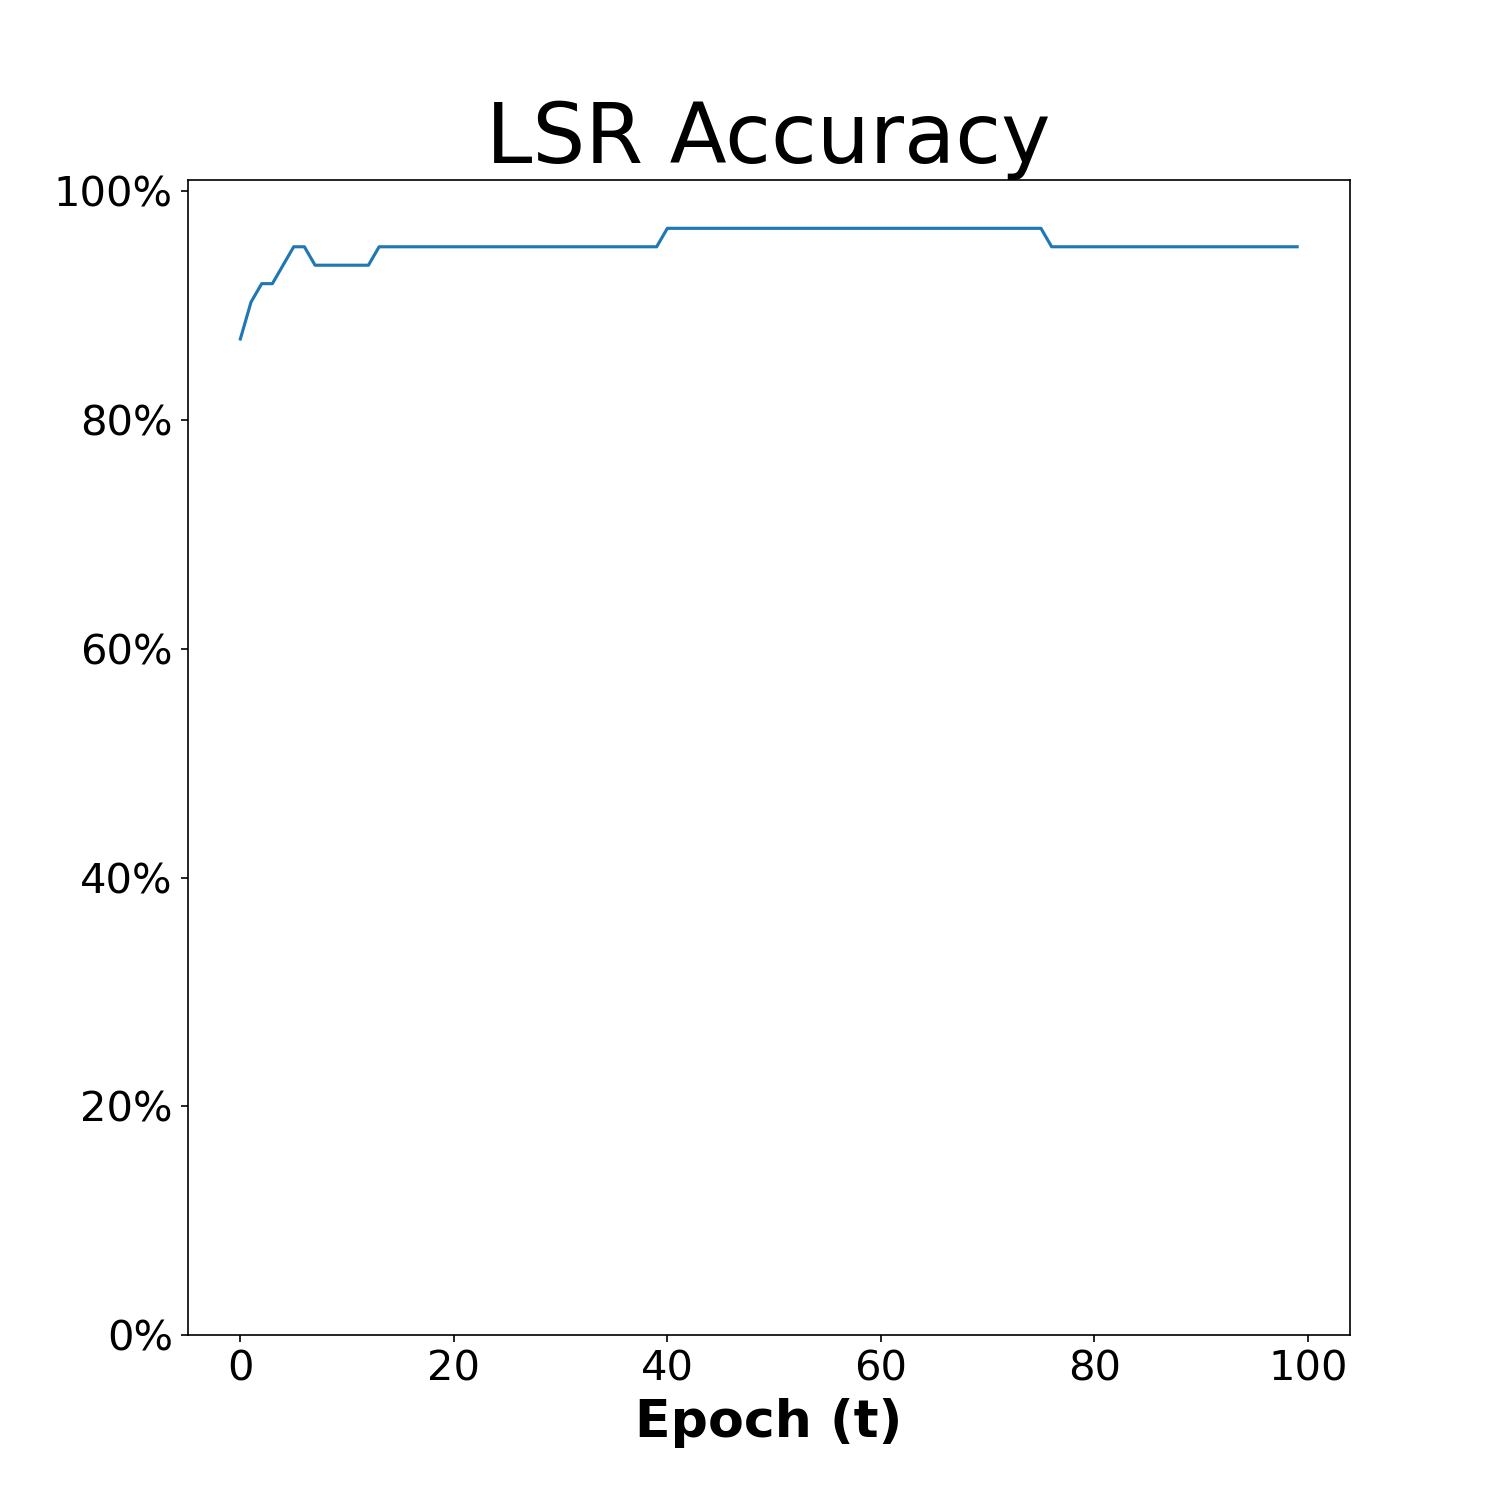
\includegraphics[width=\linewidth]{images/exper1/breast/LSR_0.01_acc.png}
    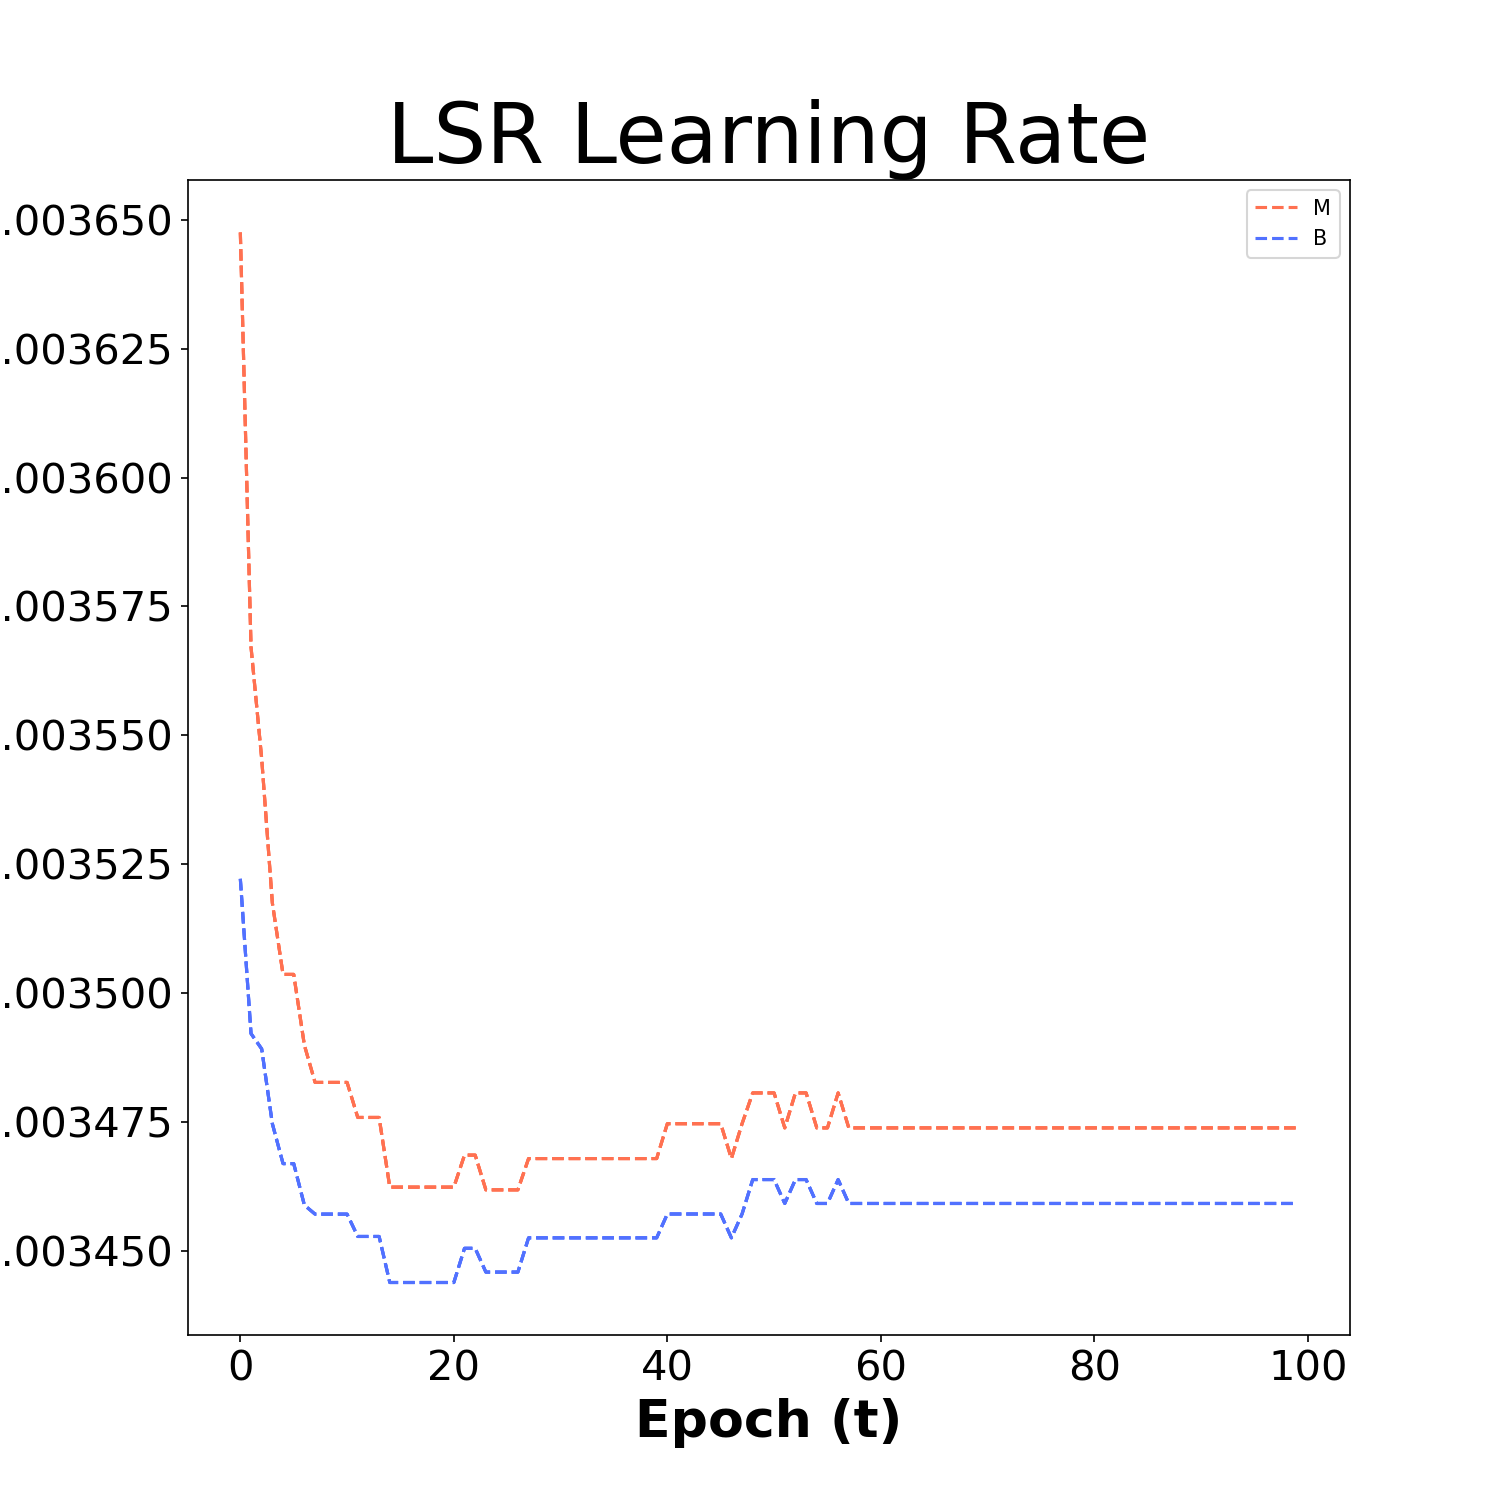
\includegraphics[width=\linewidth]{images/exper1/breast/LSR_0.01_lr.png}
  \caption{$\epsilon(0)=0.01$}
\end{subfigure}\hfil % <-- added
\begin{subfigure}{0.3\textwidth}
  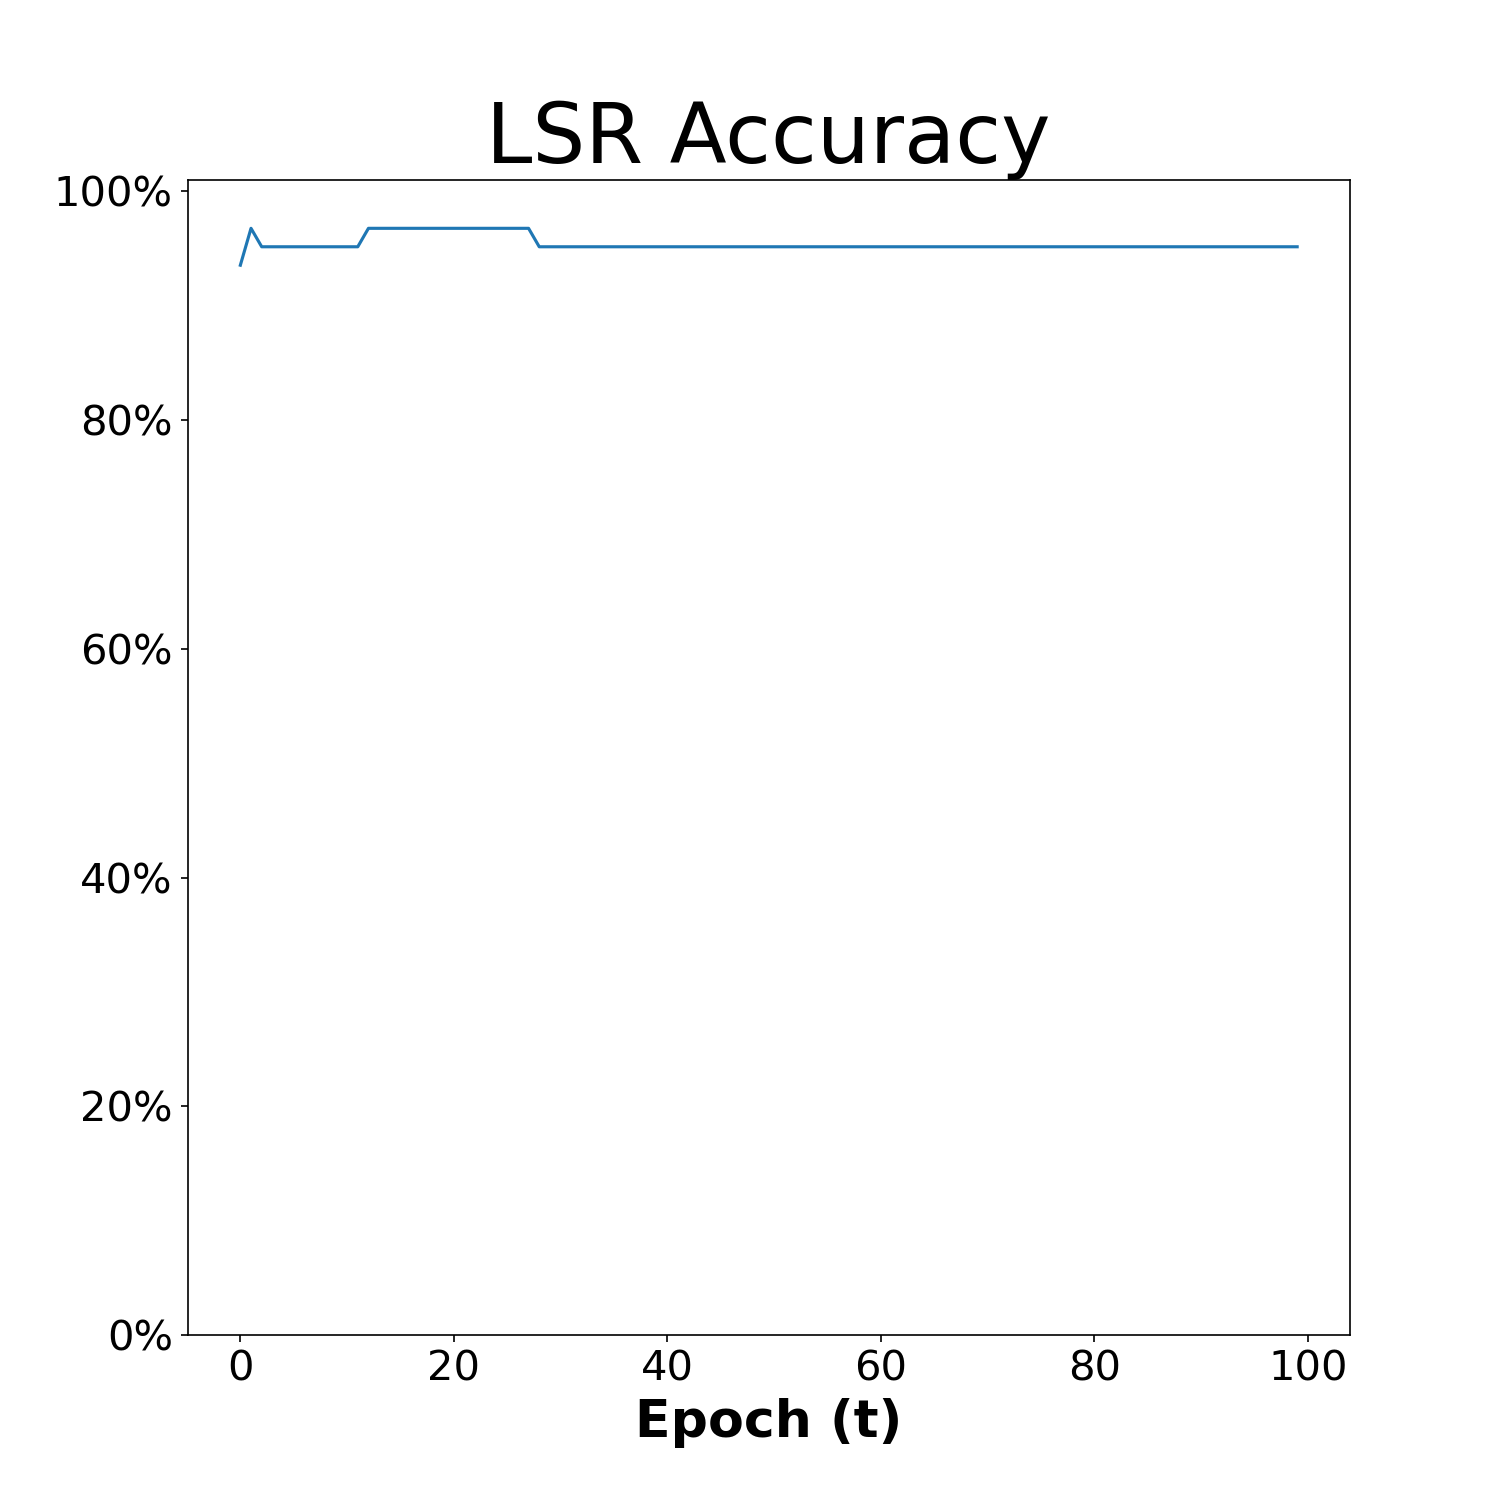
\includegraphics[width=\linewidth]{images/exper1/breast/LSR_0.03_acc.png}
  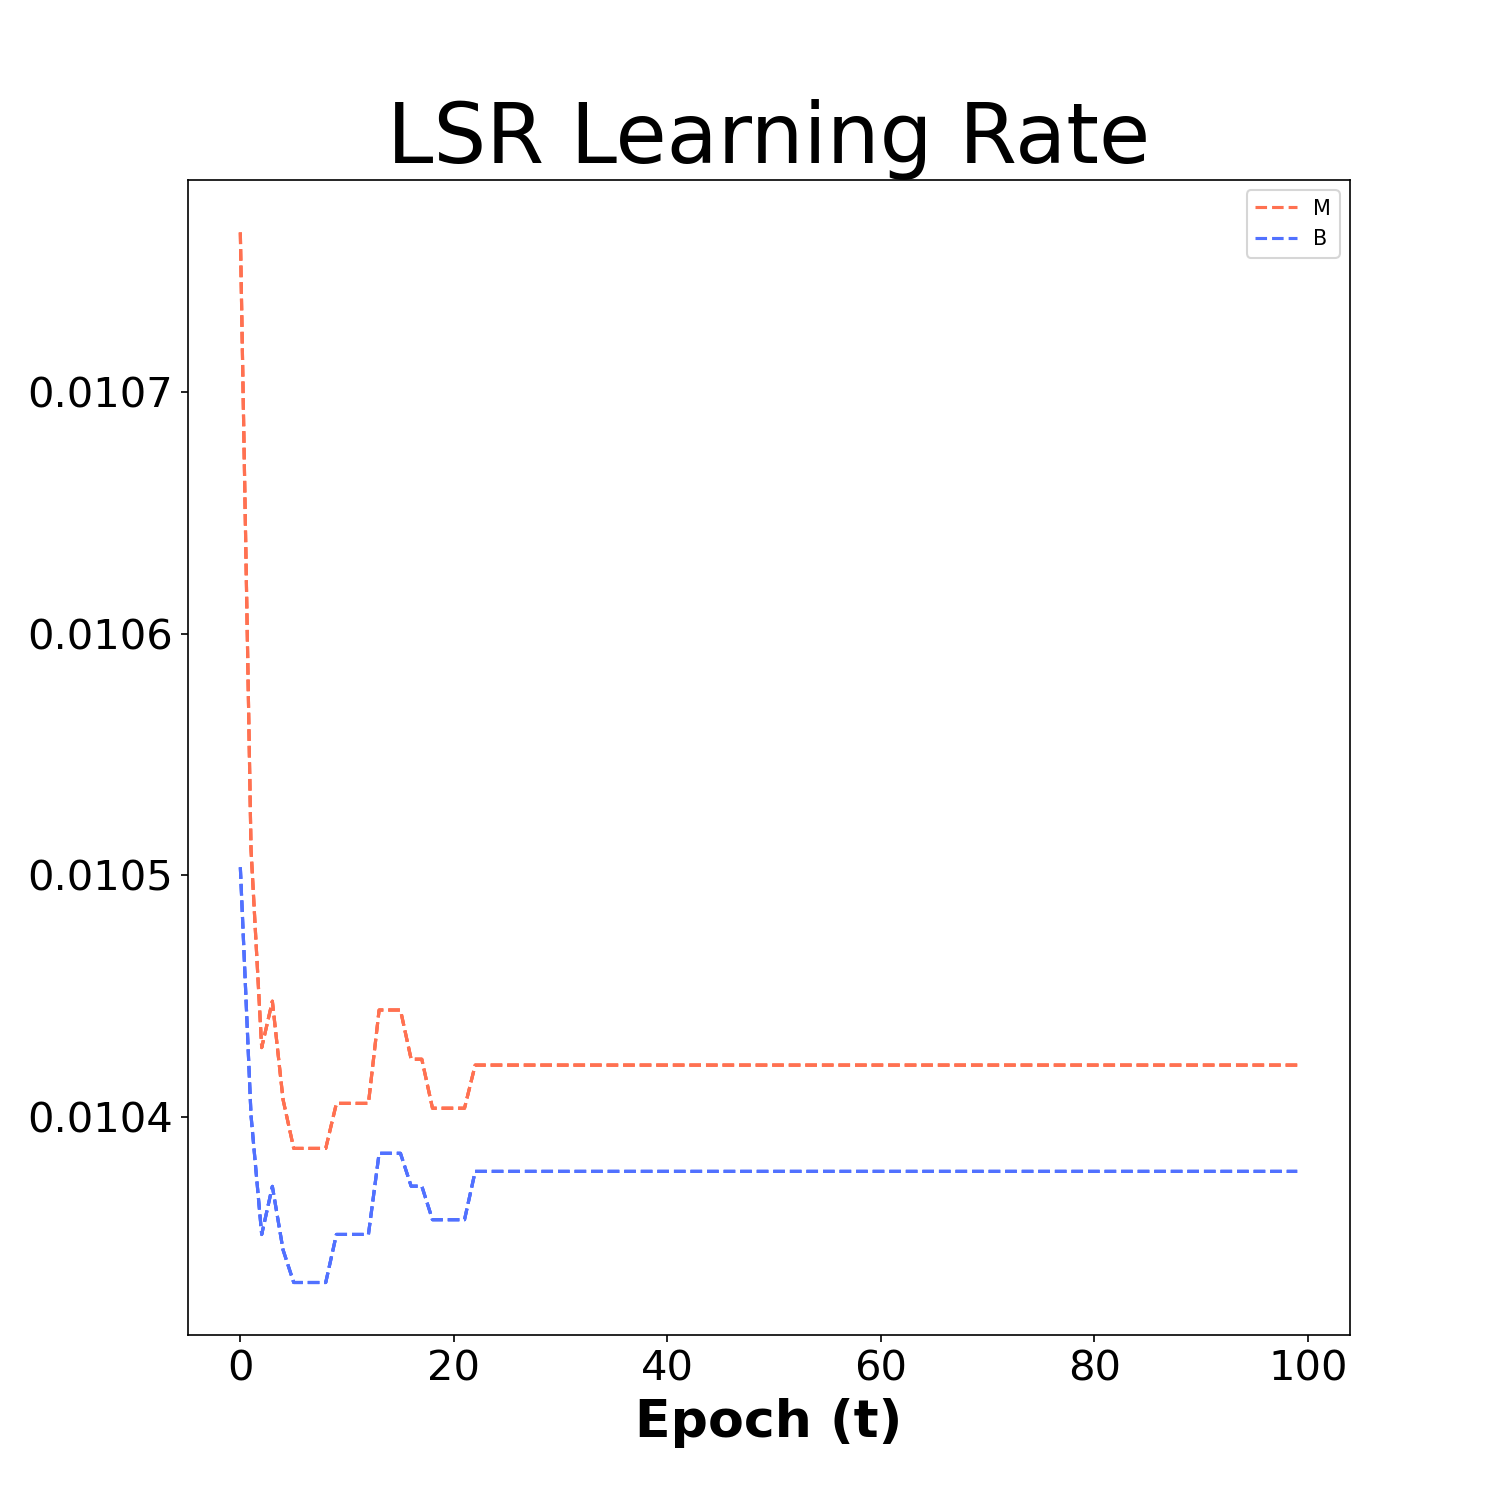
\includegraphics[width=\linewidth]{images/exper1/breast/LSR_0.03_lr.png}
  \caption{$\epsilon(0)=0.03$}
\end{subfigure}\hfil % <-- added
\begin{subfigure}{0.3\textwidth}
  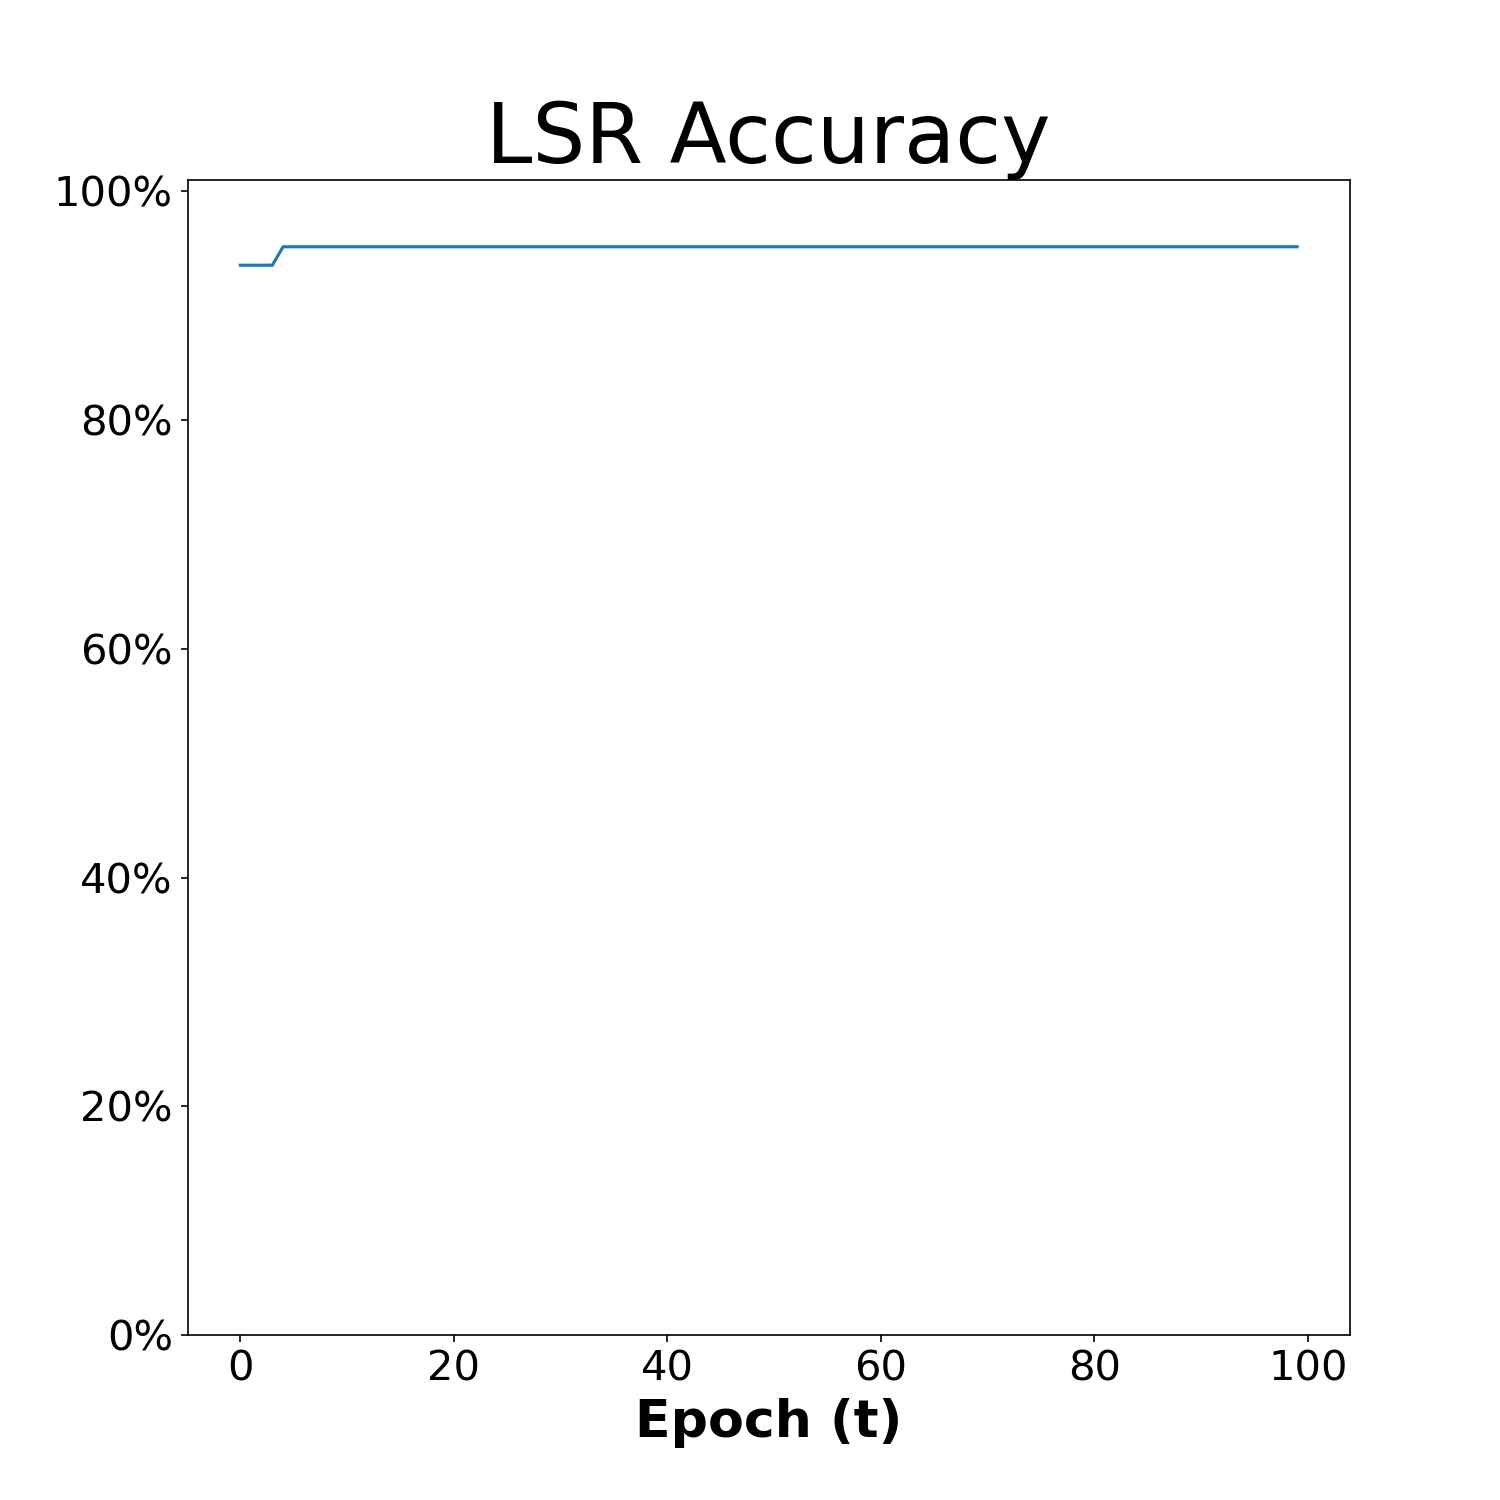
\includegraphics[width=\linewidth]{images/exper1/breast/LSR_0.1_acc.png}
  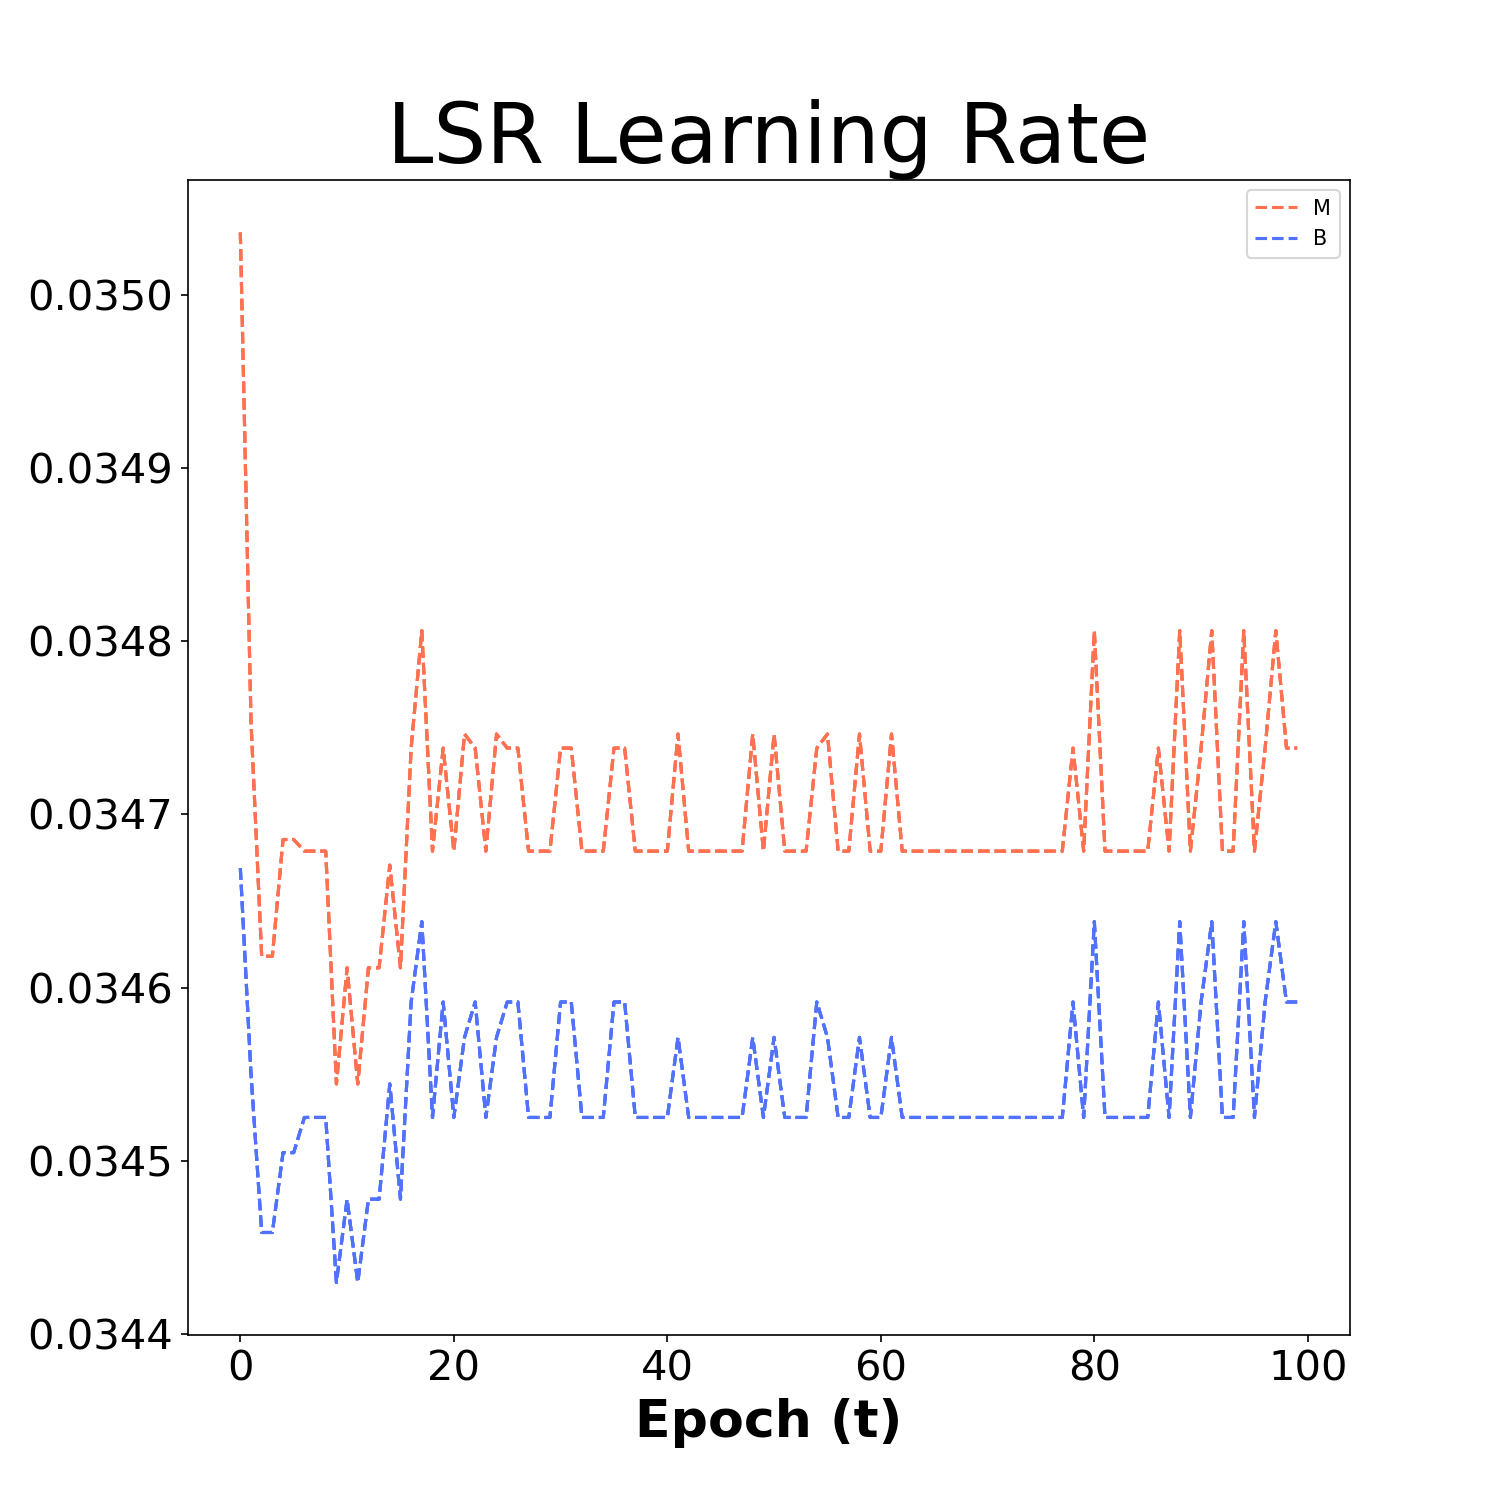
\includegraphics[width=\linewidth]{images/exper1/breast/LSR_0.1_lr.png}
  \caption{$\epsilon(0)=0.1$}
\end{subfigure}

\caption{\textit{Breast Cancer Wisconsin} dataset accuracy score and learning rate results under LSR model using balanced dataset.}
\end{figure}

\begin{figure}[H]
    \centering % <-- added
\begin{subfigure}{0.3\textwidth}
  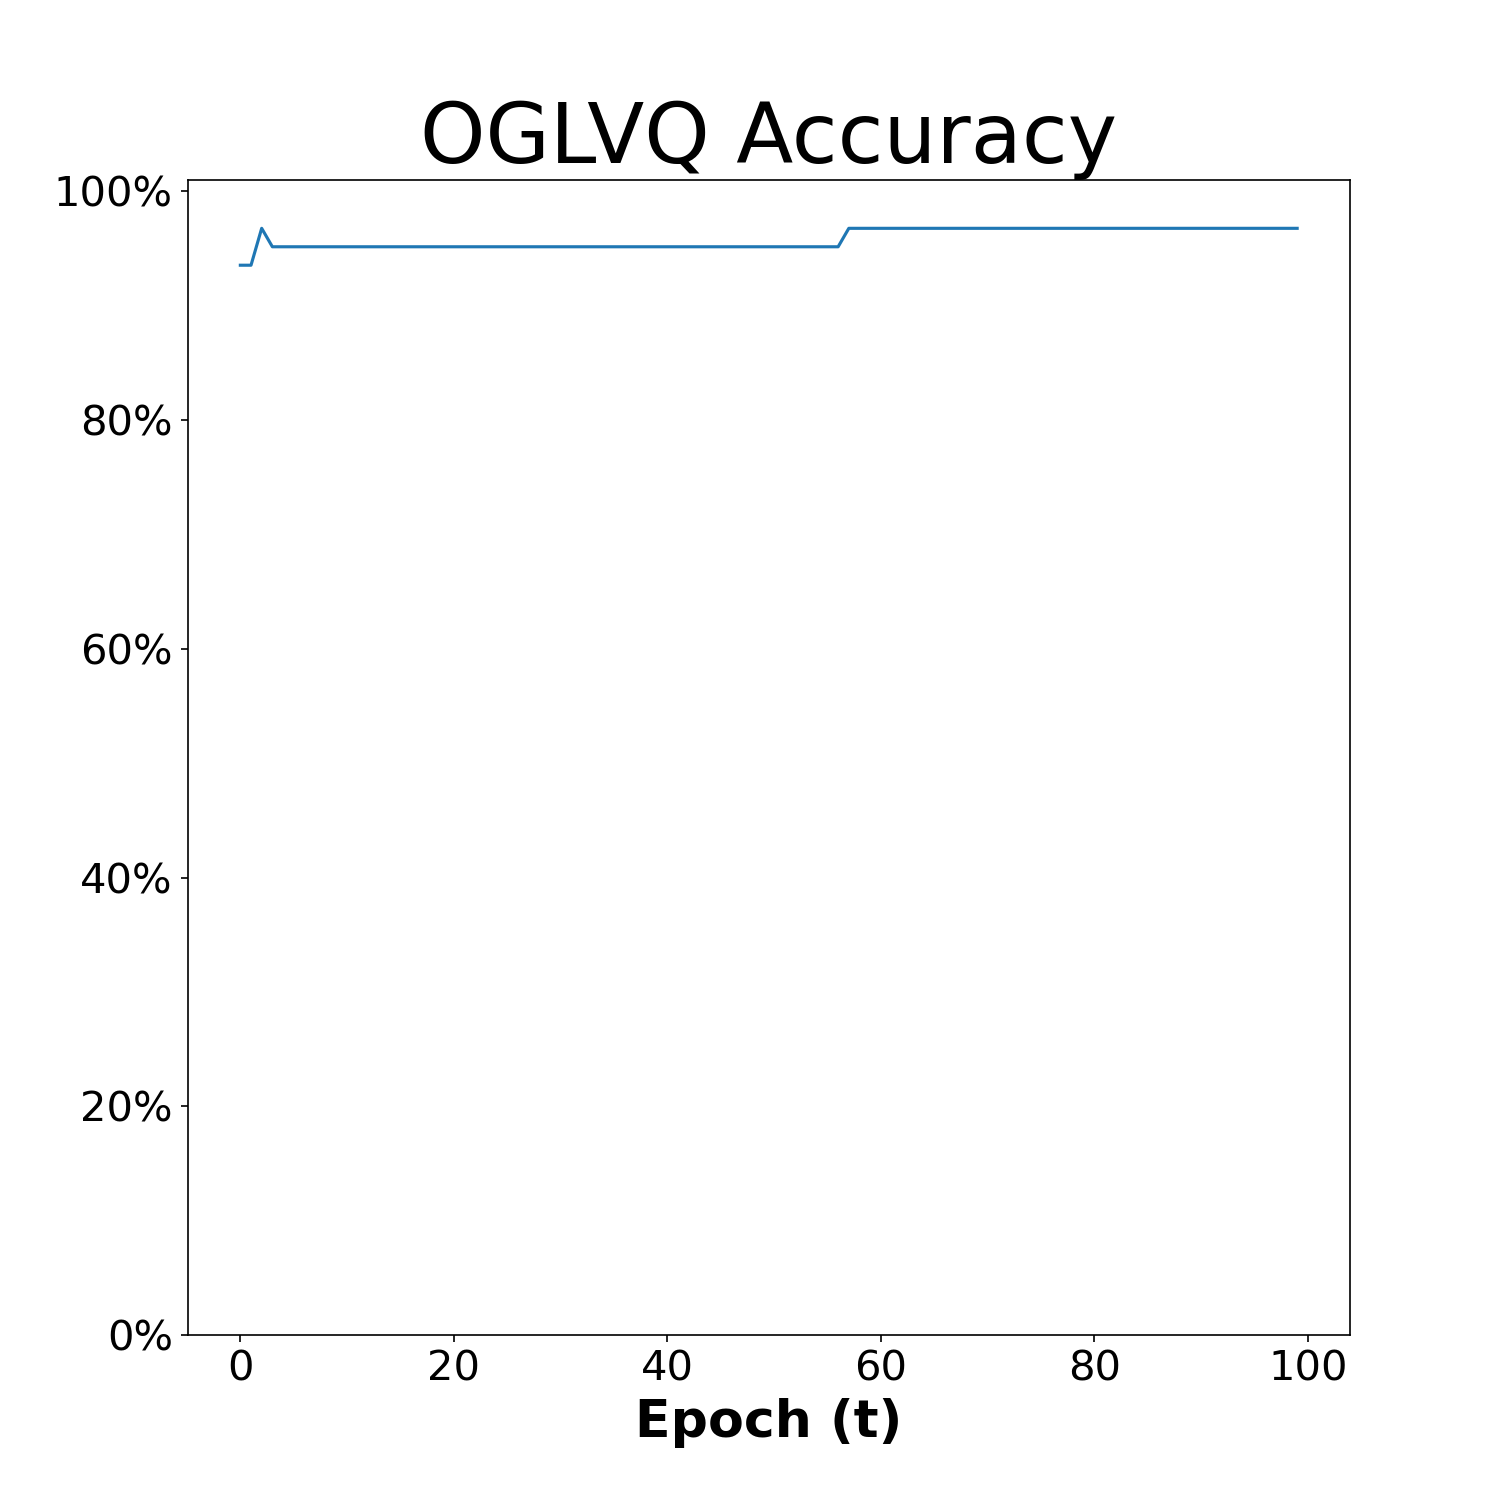
\includegraphics[width=\linewidth]{images/exper1/breast/OGLVQ_0.01_acc.png}
    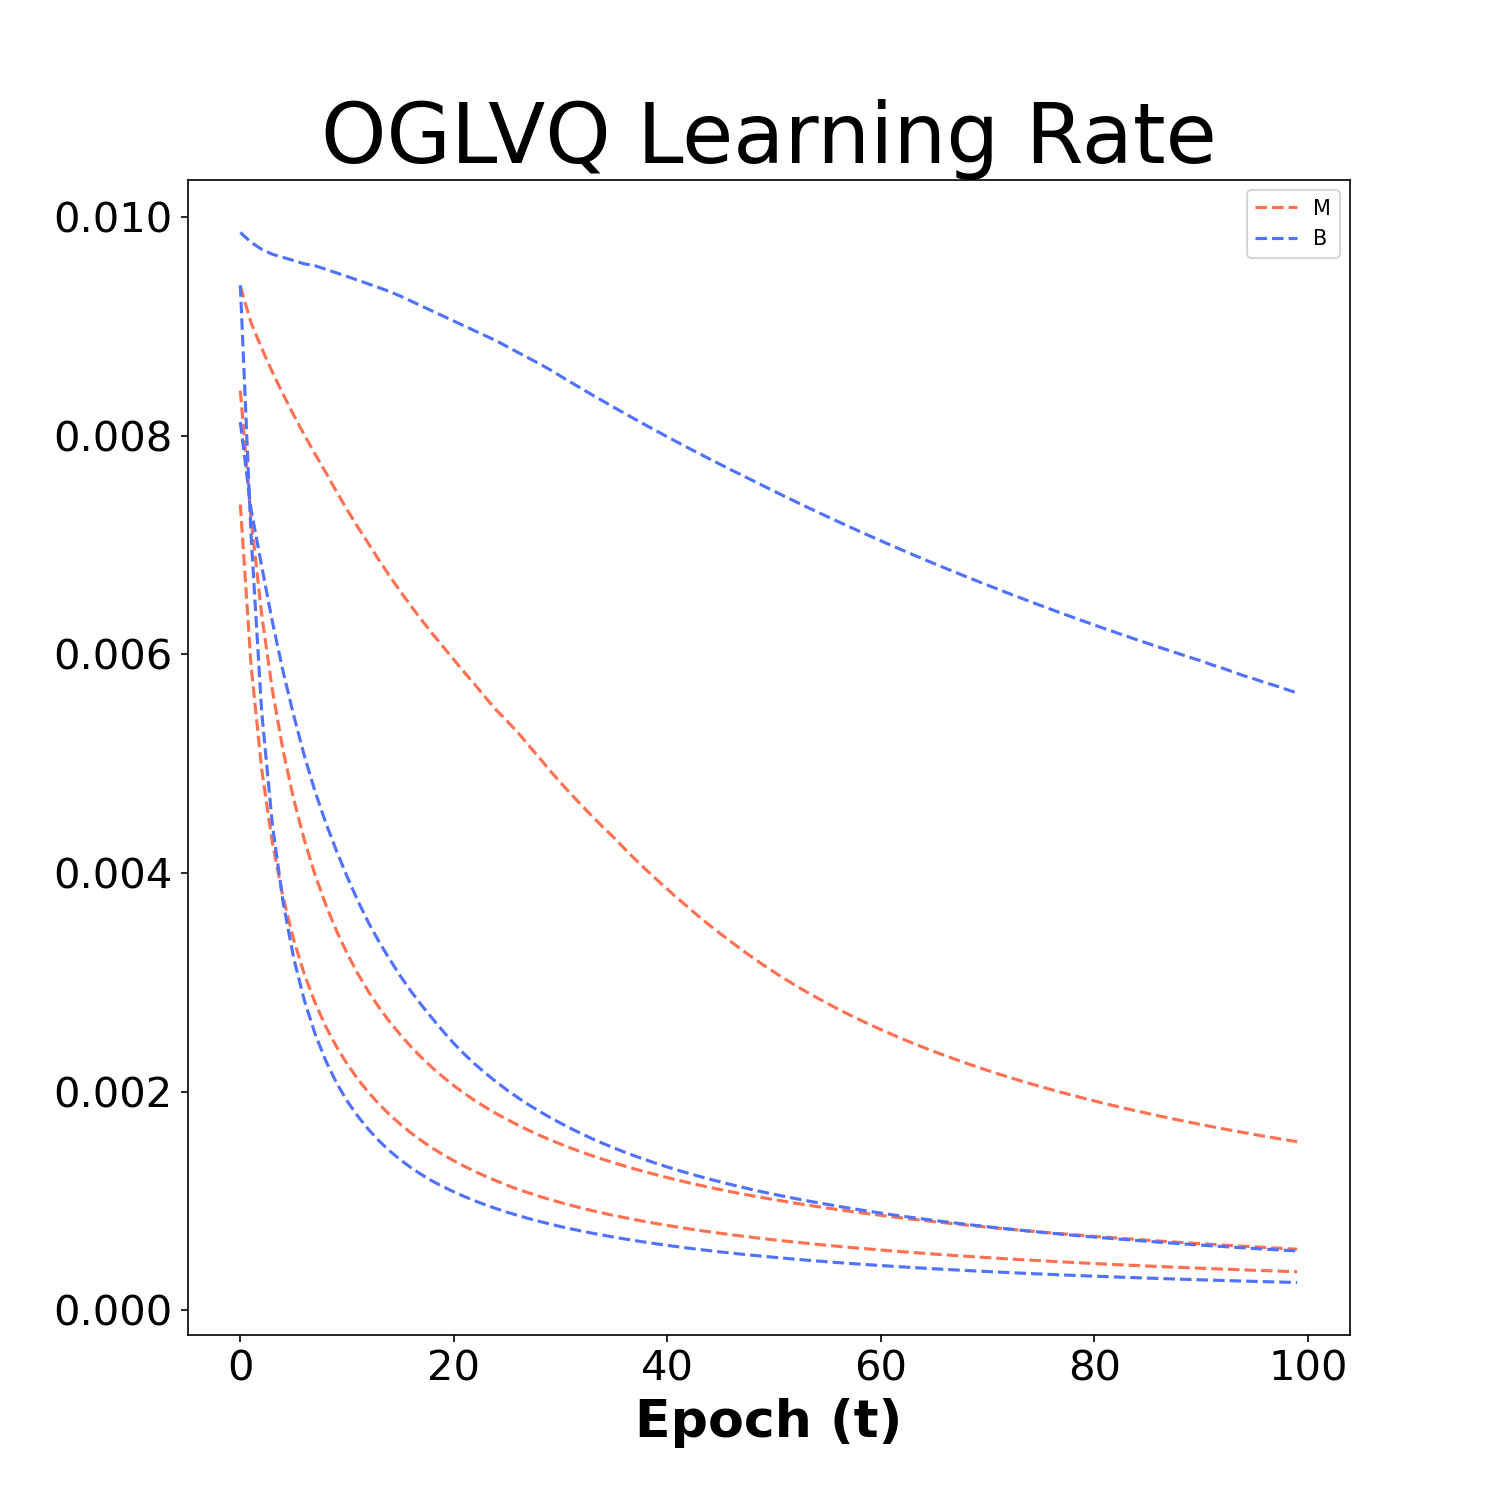
\includegraphics[width=\linewidth]{images/exper1/breast/OGLVQ_0.01_lr.png}
  \caption{$\epsilon(0)=0.01$}
\end{subfigure}\hfil % <-- added
\begin{subfigure}{0.3\textwidth}
  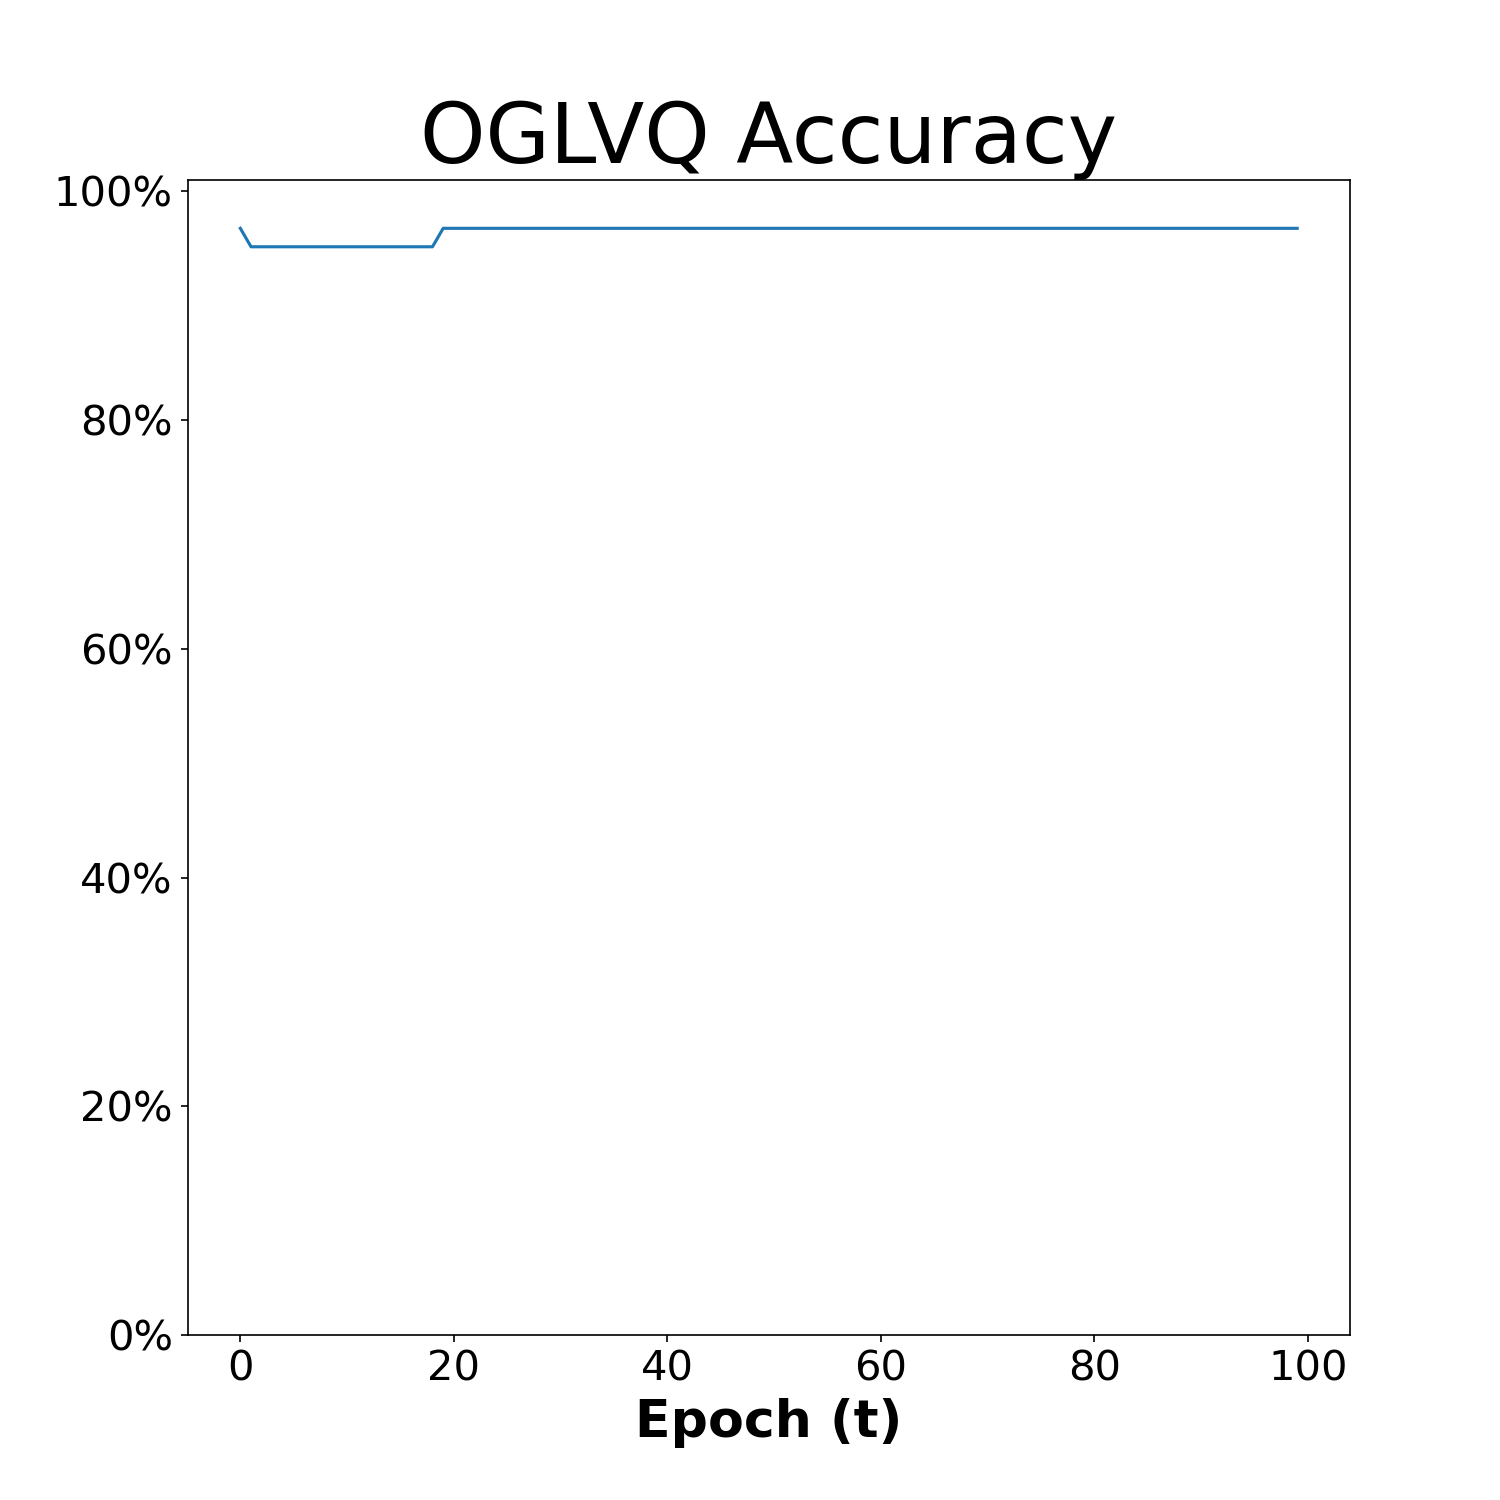
\includegraphics[width=\linewidth]{images/exper1/breast/OGLVQ_0.03_acc.png}
  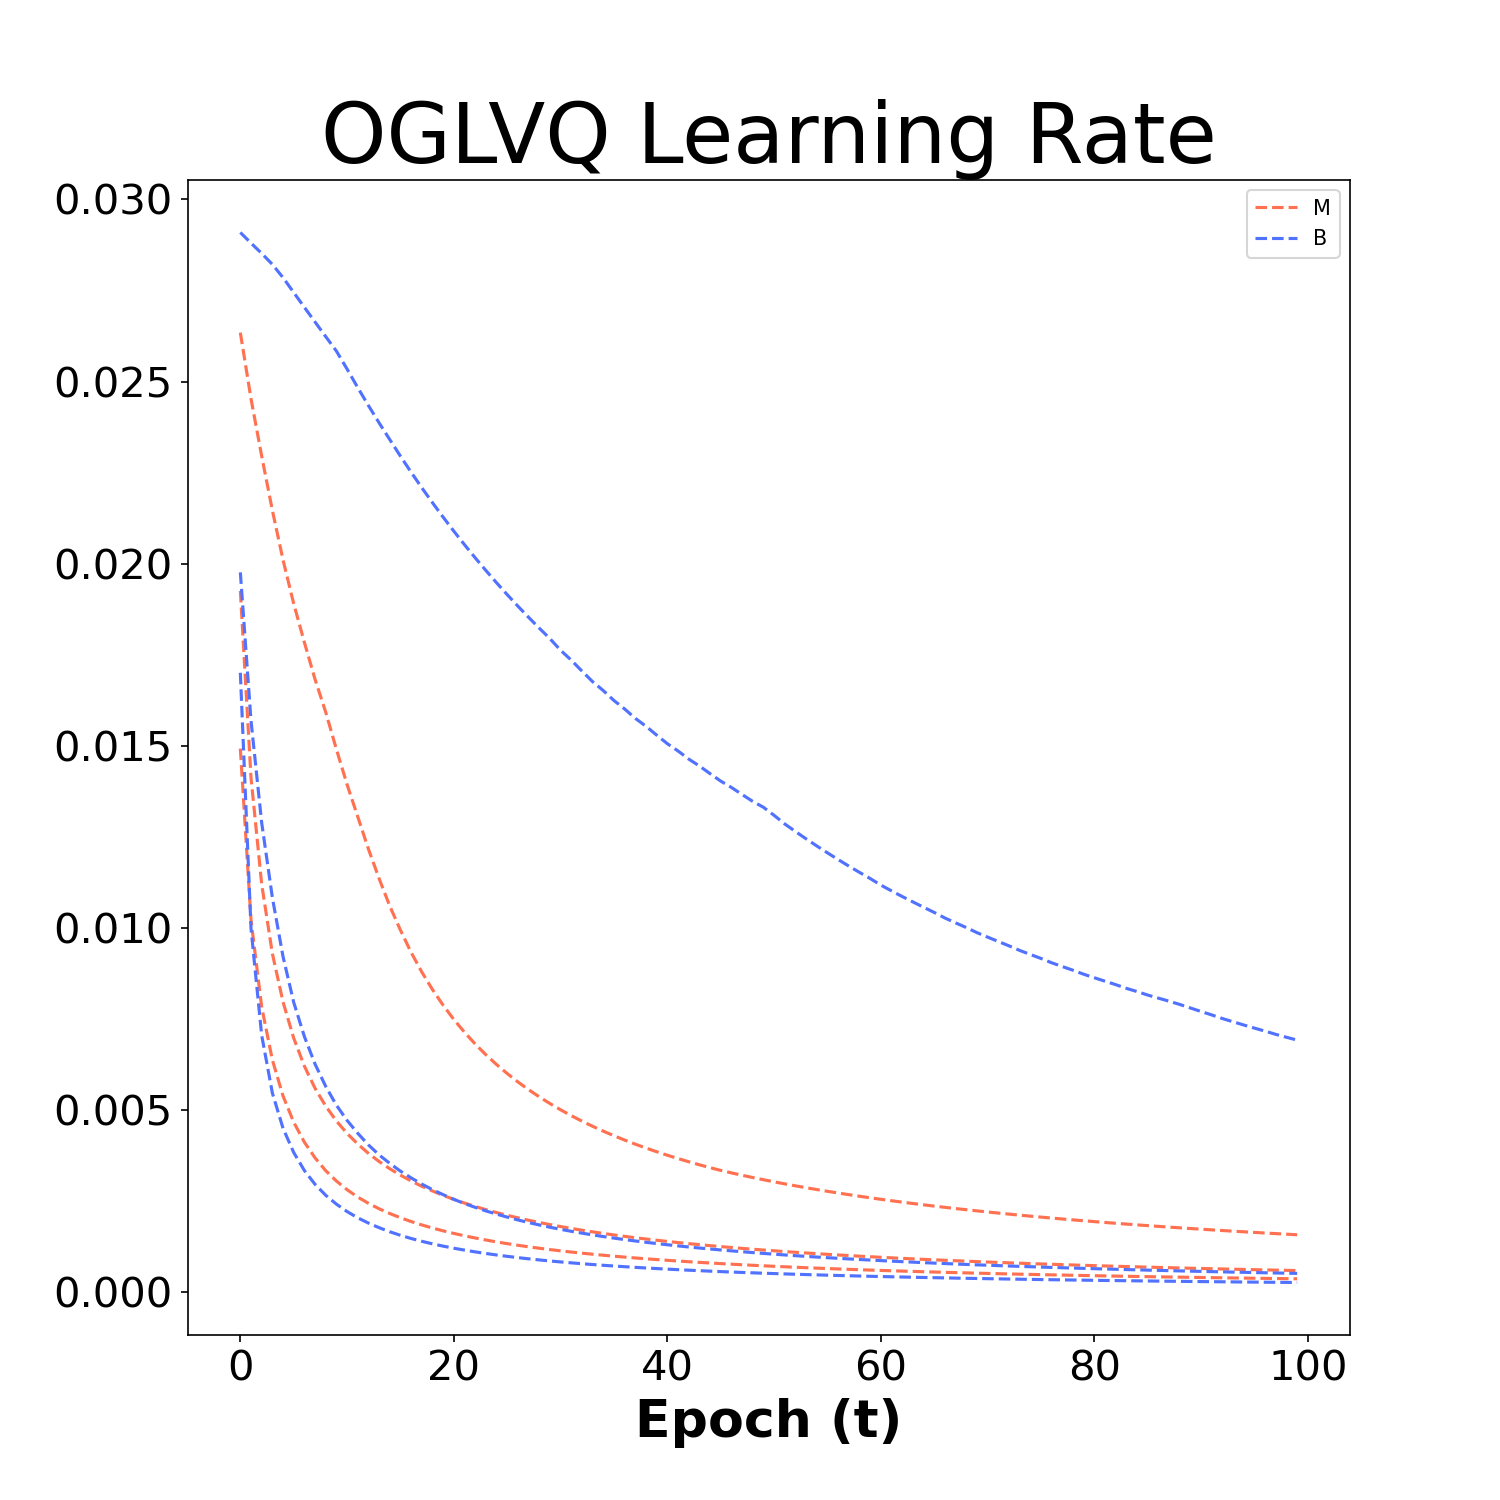
\includegraphics[width=\linewidth]{images/exper1/breast/OGLVQ_0.03_lr.png}
  \caption{$\epsilon(0)=0.03$}
\end{subfigure}\hfil % <-- added
\begin{subfigure}{0.3\textwidth}
  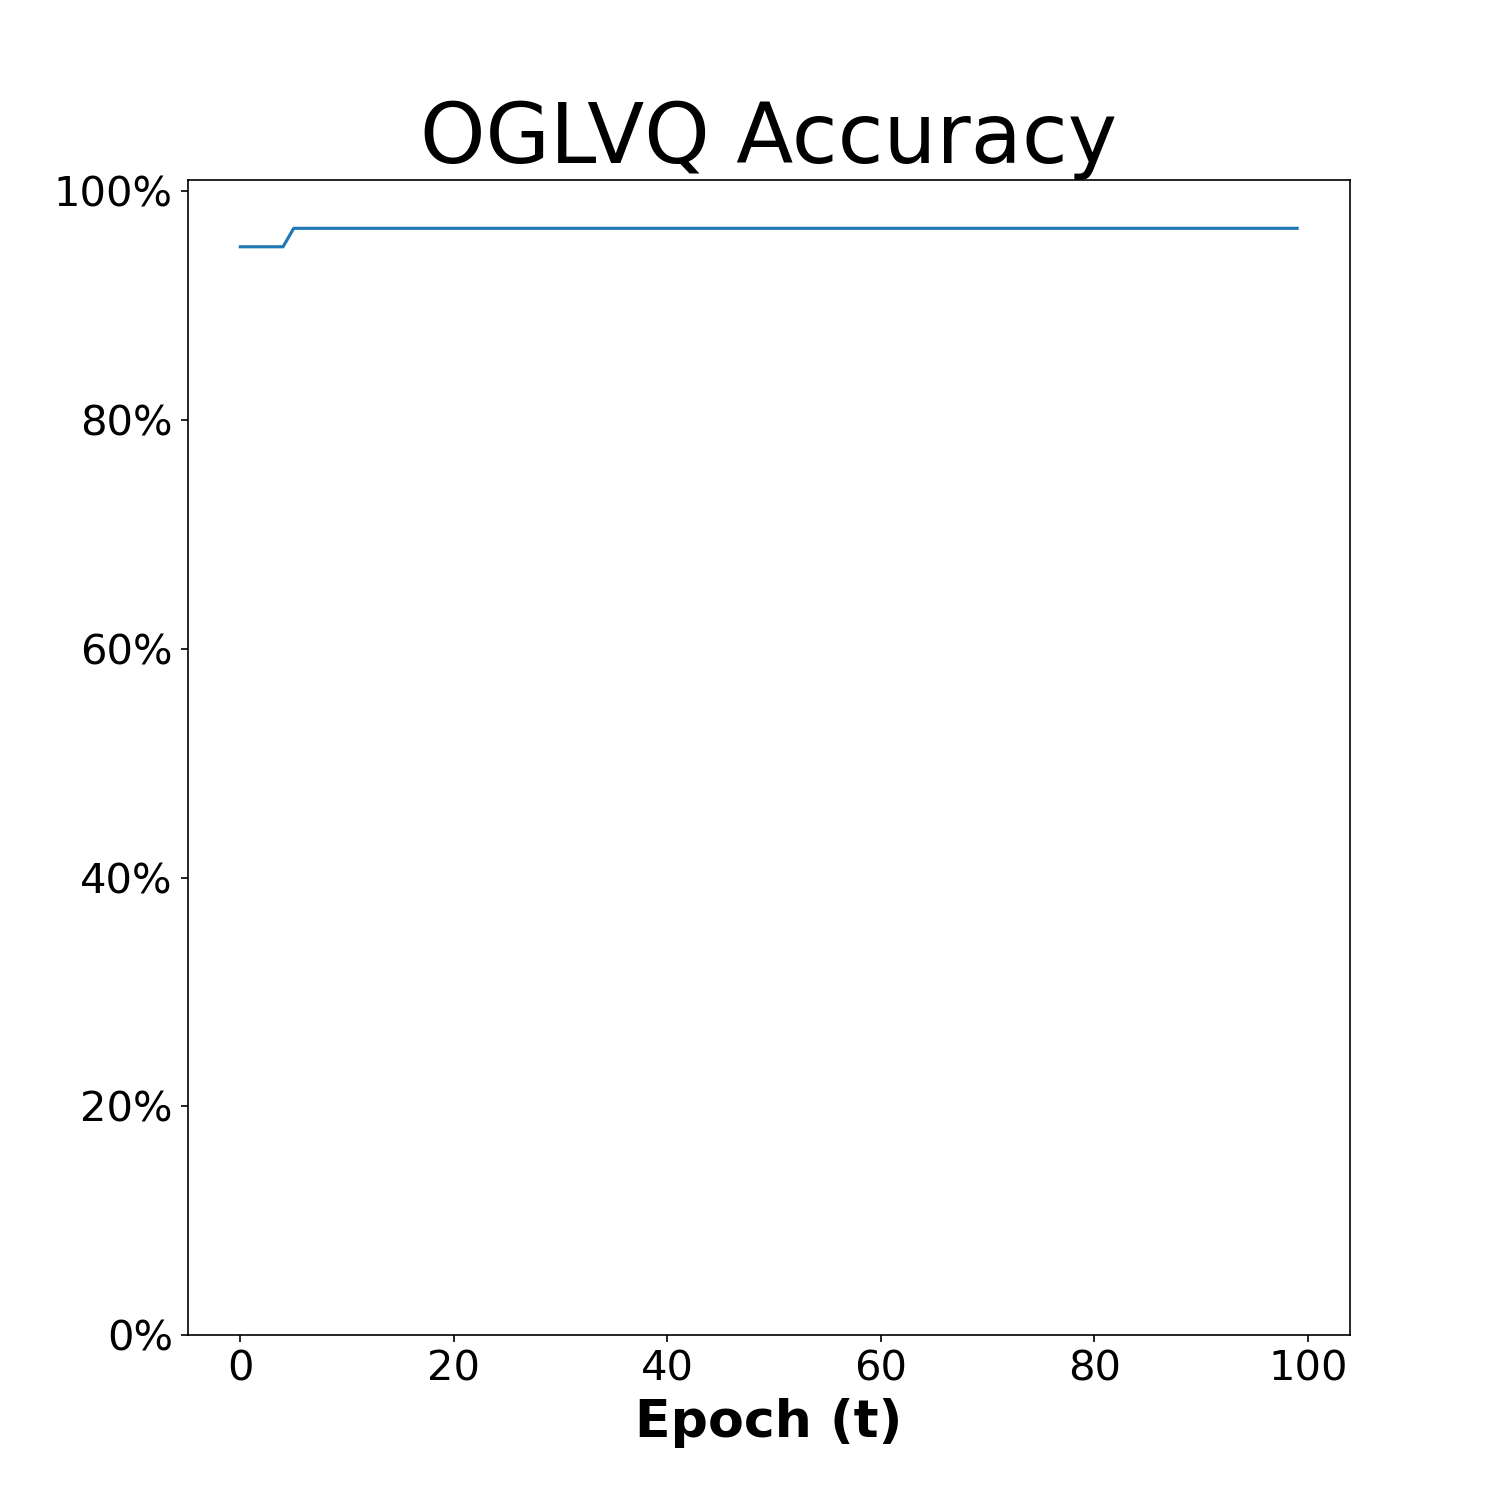
\includegraphics[width=\linewidth]{images/exper1/breast/OGLVQ_0.1_acc.png}
  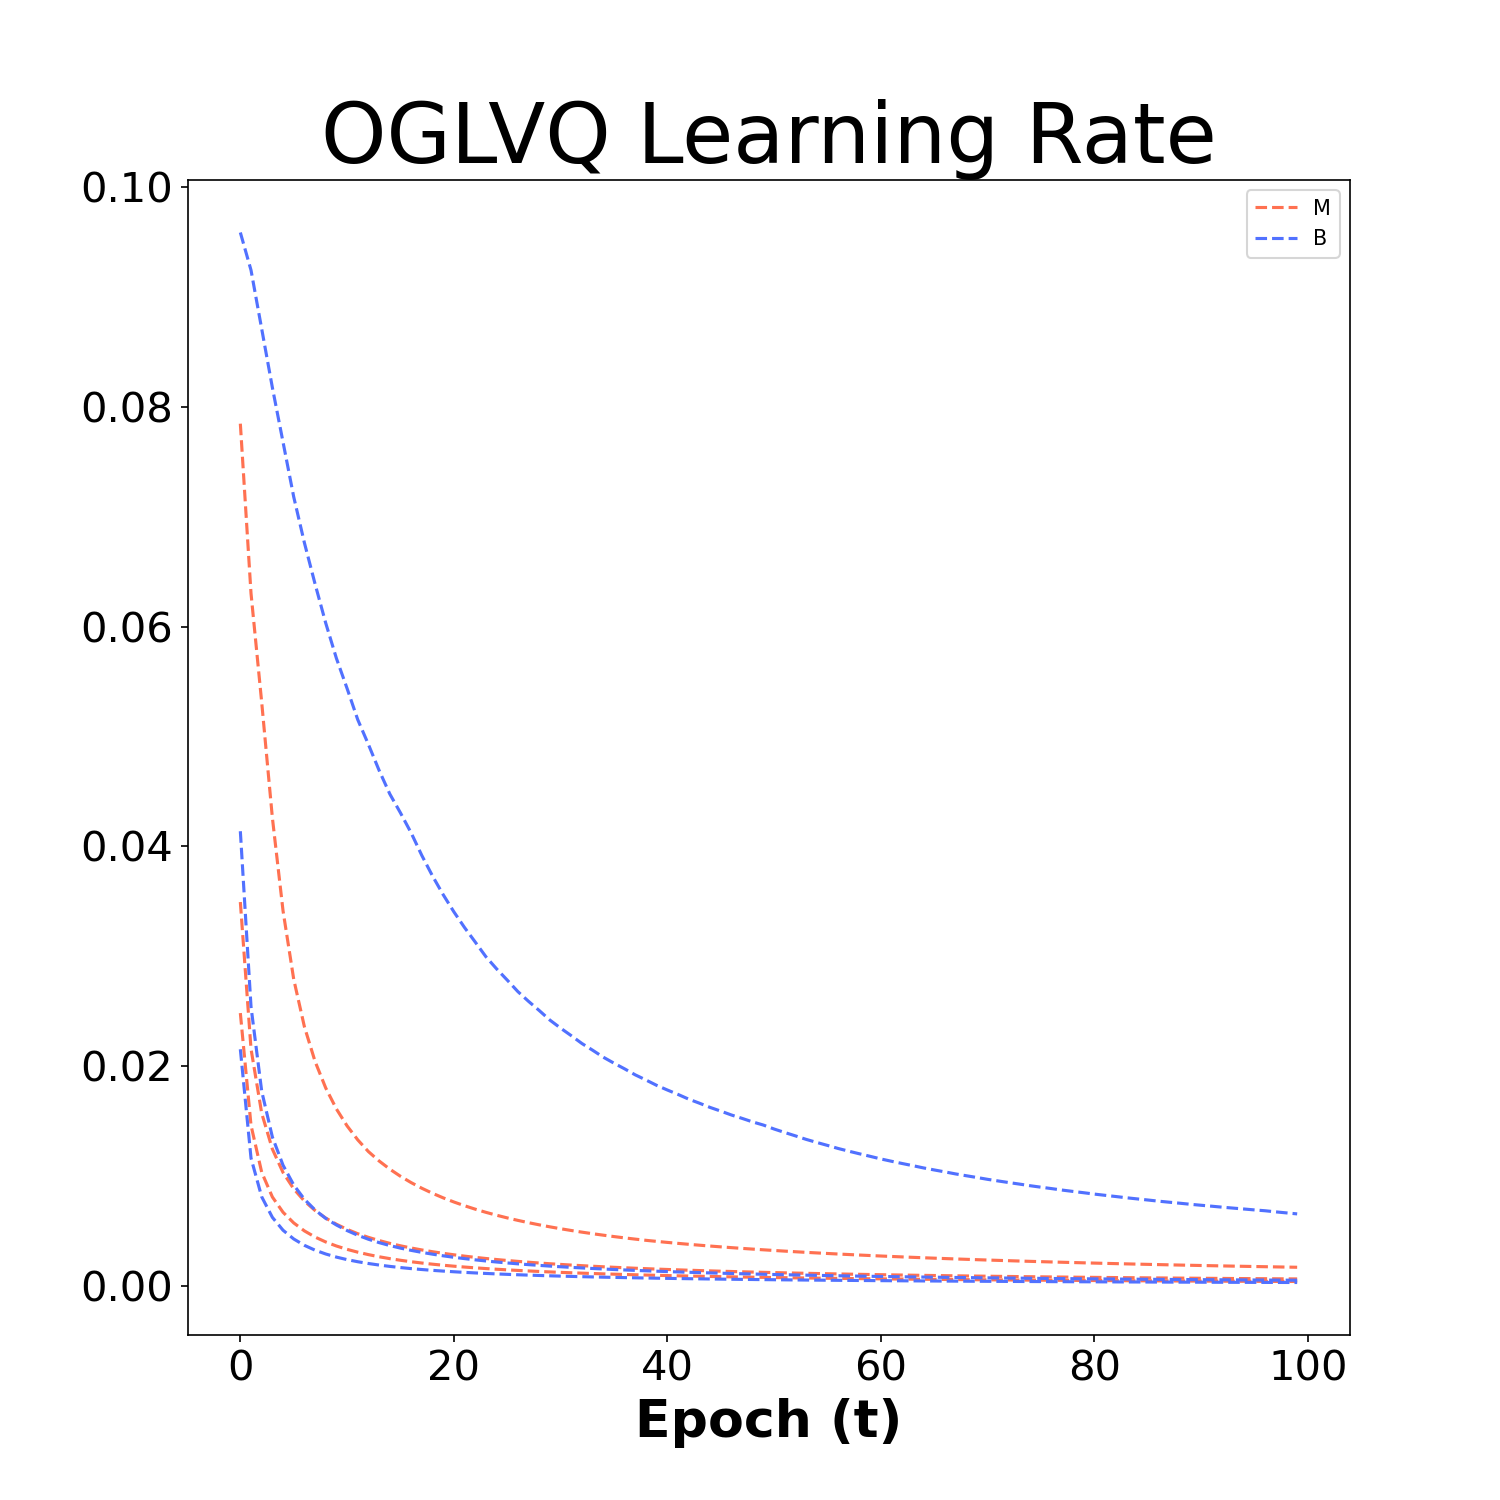
\includegraphics[width=\linewidth]{images/exper1/breast/OGLVQ_0.1_lr.png}
  \caption{$\epsilon(0)=0.1$}
\end{subfigure}

\caption{\textit{Breast Cancer Wisconsin} dataset accuracy score and learning rate results under OGLVQ model using balanced dataset.}
\end{figure}




\subsection{Iris dataset}

Prototypes for each class: 3
\vspace{5pt}


If we check the results of the \textit{Iris} dataset, we see all models’ accuracy scores start at 1 for at least one initial rate test. That indicates the dataset is already divided nicely for classification. Even though accuracy is high initially, that does not mean the model cannot learn. The model tries to find a nice line between data samples to divide samples as perfectly as possible. We see some decrease in accuracy scores of the CP model for any $\epsilon(0)$, which also affects the $\epsilon_{i}$ values during the training of the experiment. With accuracy getting lower, $\epsilon_{i}$ for all prototypes get higher, which indicates the model is learning badly. It classifies worse with every epoch that passes. For other CGLVQ models, we see that accuracies are stable at high accuracy scores, between 90\% and 100\%. Besides, the learning rates stuck in a constant value (for DFH($\epsilon(0)=0.01$), DFH($\epsilon(0)=0.1$), MS($\epsilon(0)=0.1$), LS($\epsilon(0)=0.1$), LSR($\epsilon(0)=0.01$), LSR($\epsilon(0)=0.1$)) or zigzagging between a value range (for DFH($\epsilon(0)=0.03$), MS($\epsilon(0)=0.01$), MS($\epsilon(0)=0.03$), LS($\epsilon(0)=0.01$), LS($\epsilon(0)=0.03$), LSR($\epsilon(0)=0.03$)). We can interpret this zigzagging effect as the model is indecisive about where to draw the line between the classes since at least one test sample is close to two different classes, and prototypes cannot decide. So, there is not much learning going on in CGLVQ models. However, in the OGLVQ model with low $\epsilon(0)$ such as 0.01 and 0.03, we see better $\epsilon_{i}$ curves diminishing to 0, indicating that the model adapts and learns greatly.


\begin{figure}[H]
    \centering
    \begin{subfigure}[t]{0.45\textwidth}
        \centering
        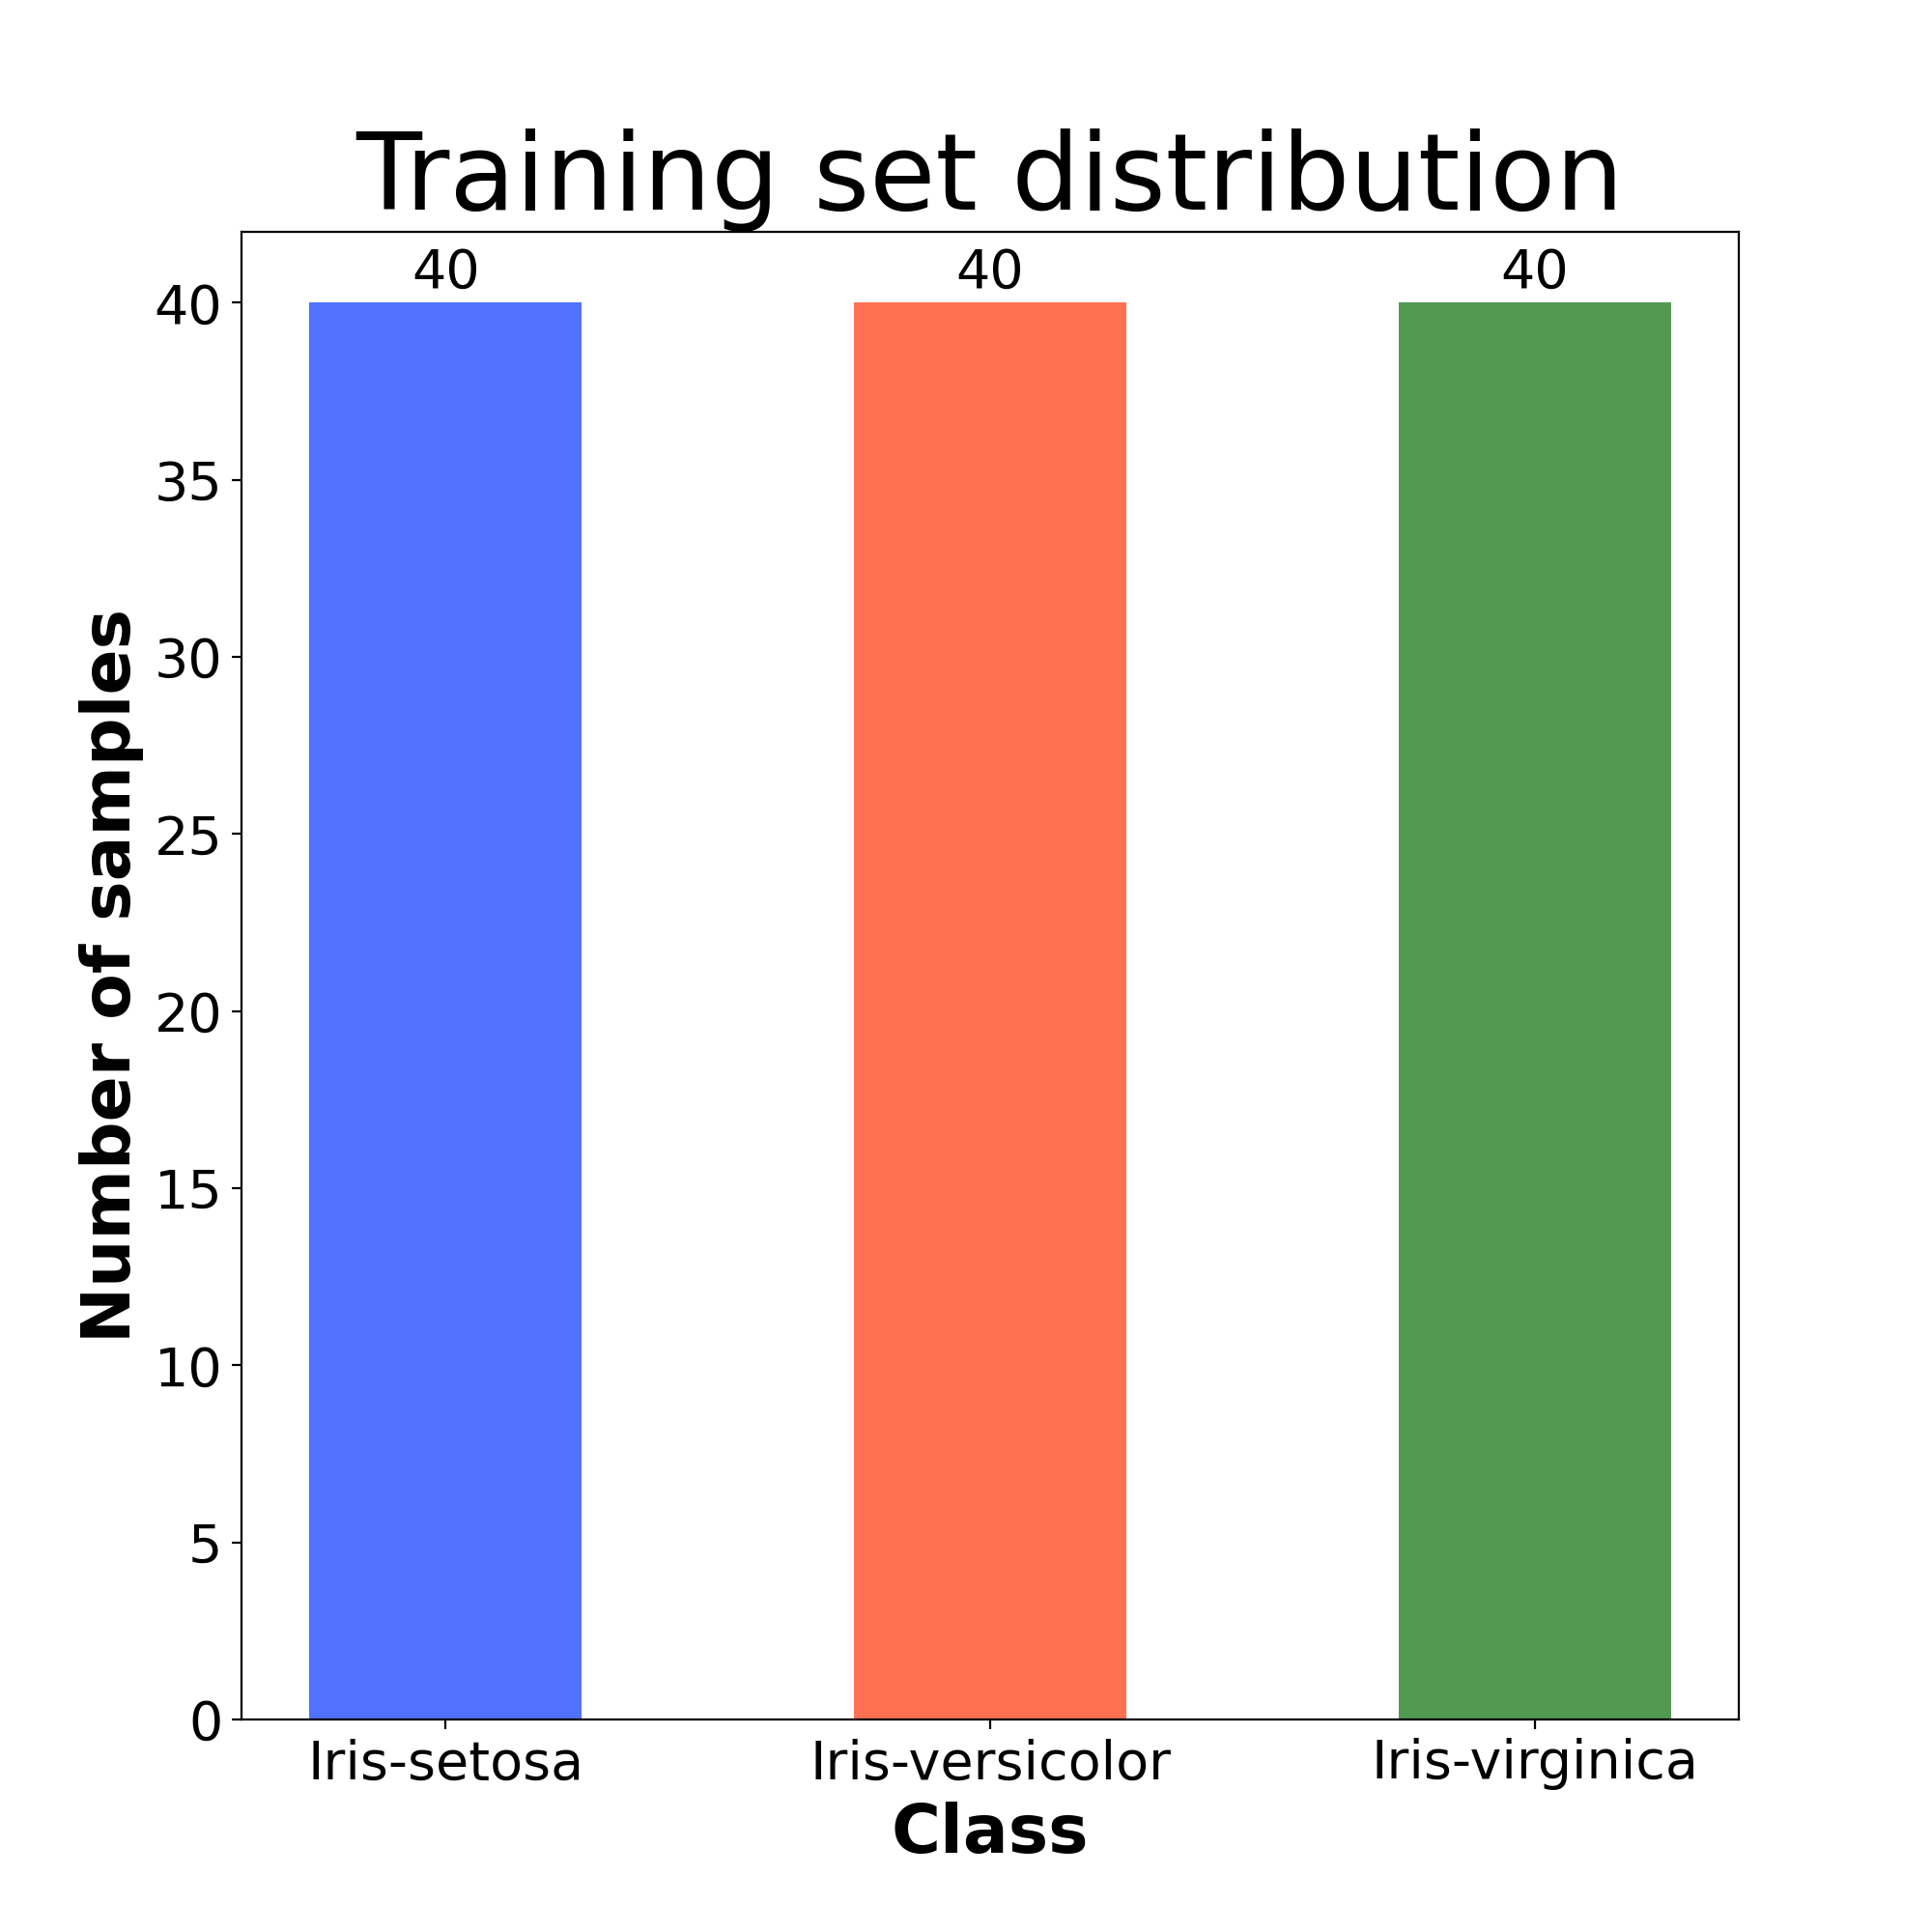
\includegraphics[width=1\textwidth]{images/exper1/iris/train_dist.png}
        \caption{Training set}
    \end{subfigure}
    \begin{subfigure}[t]{0.45\textwidth}
        \centering
        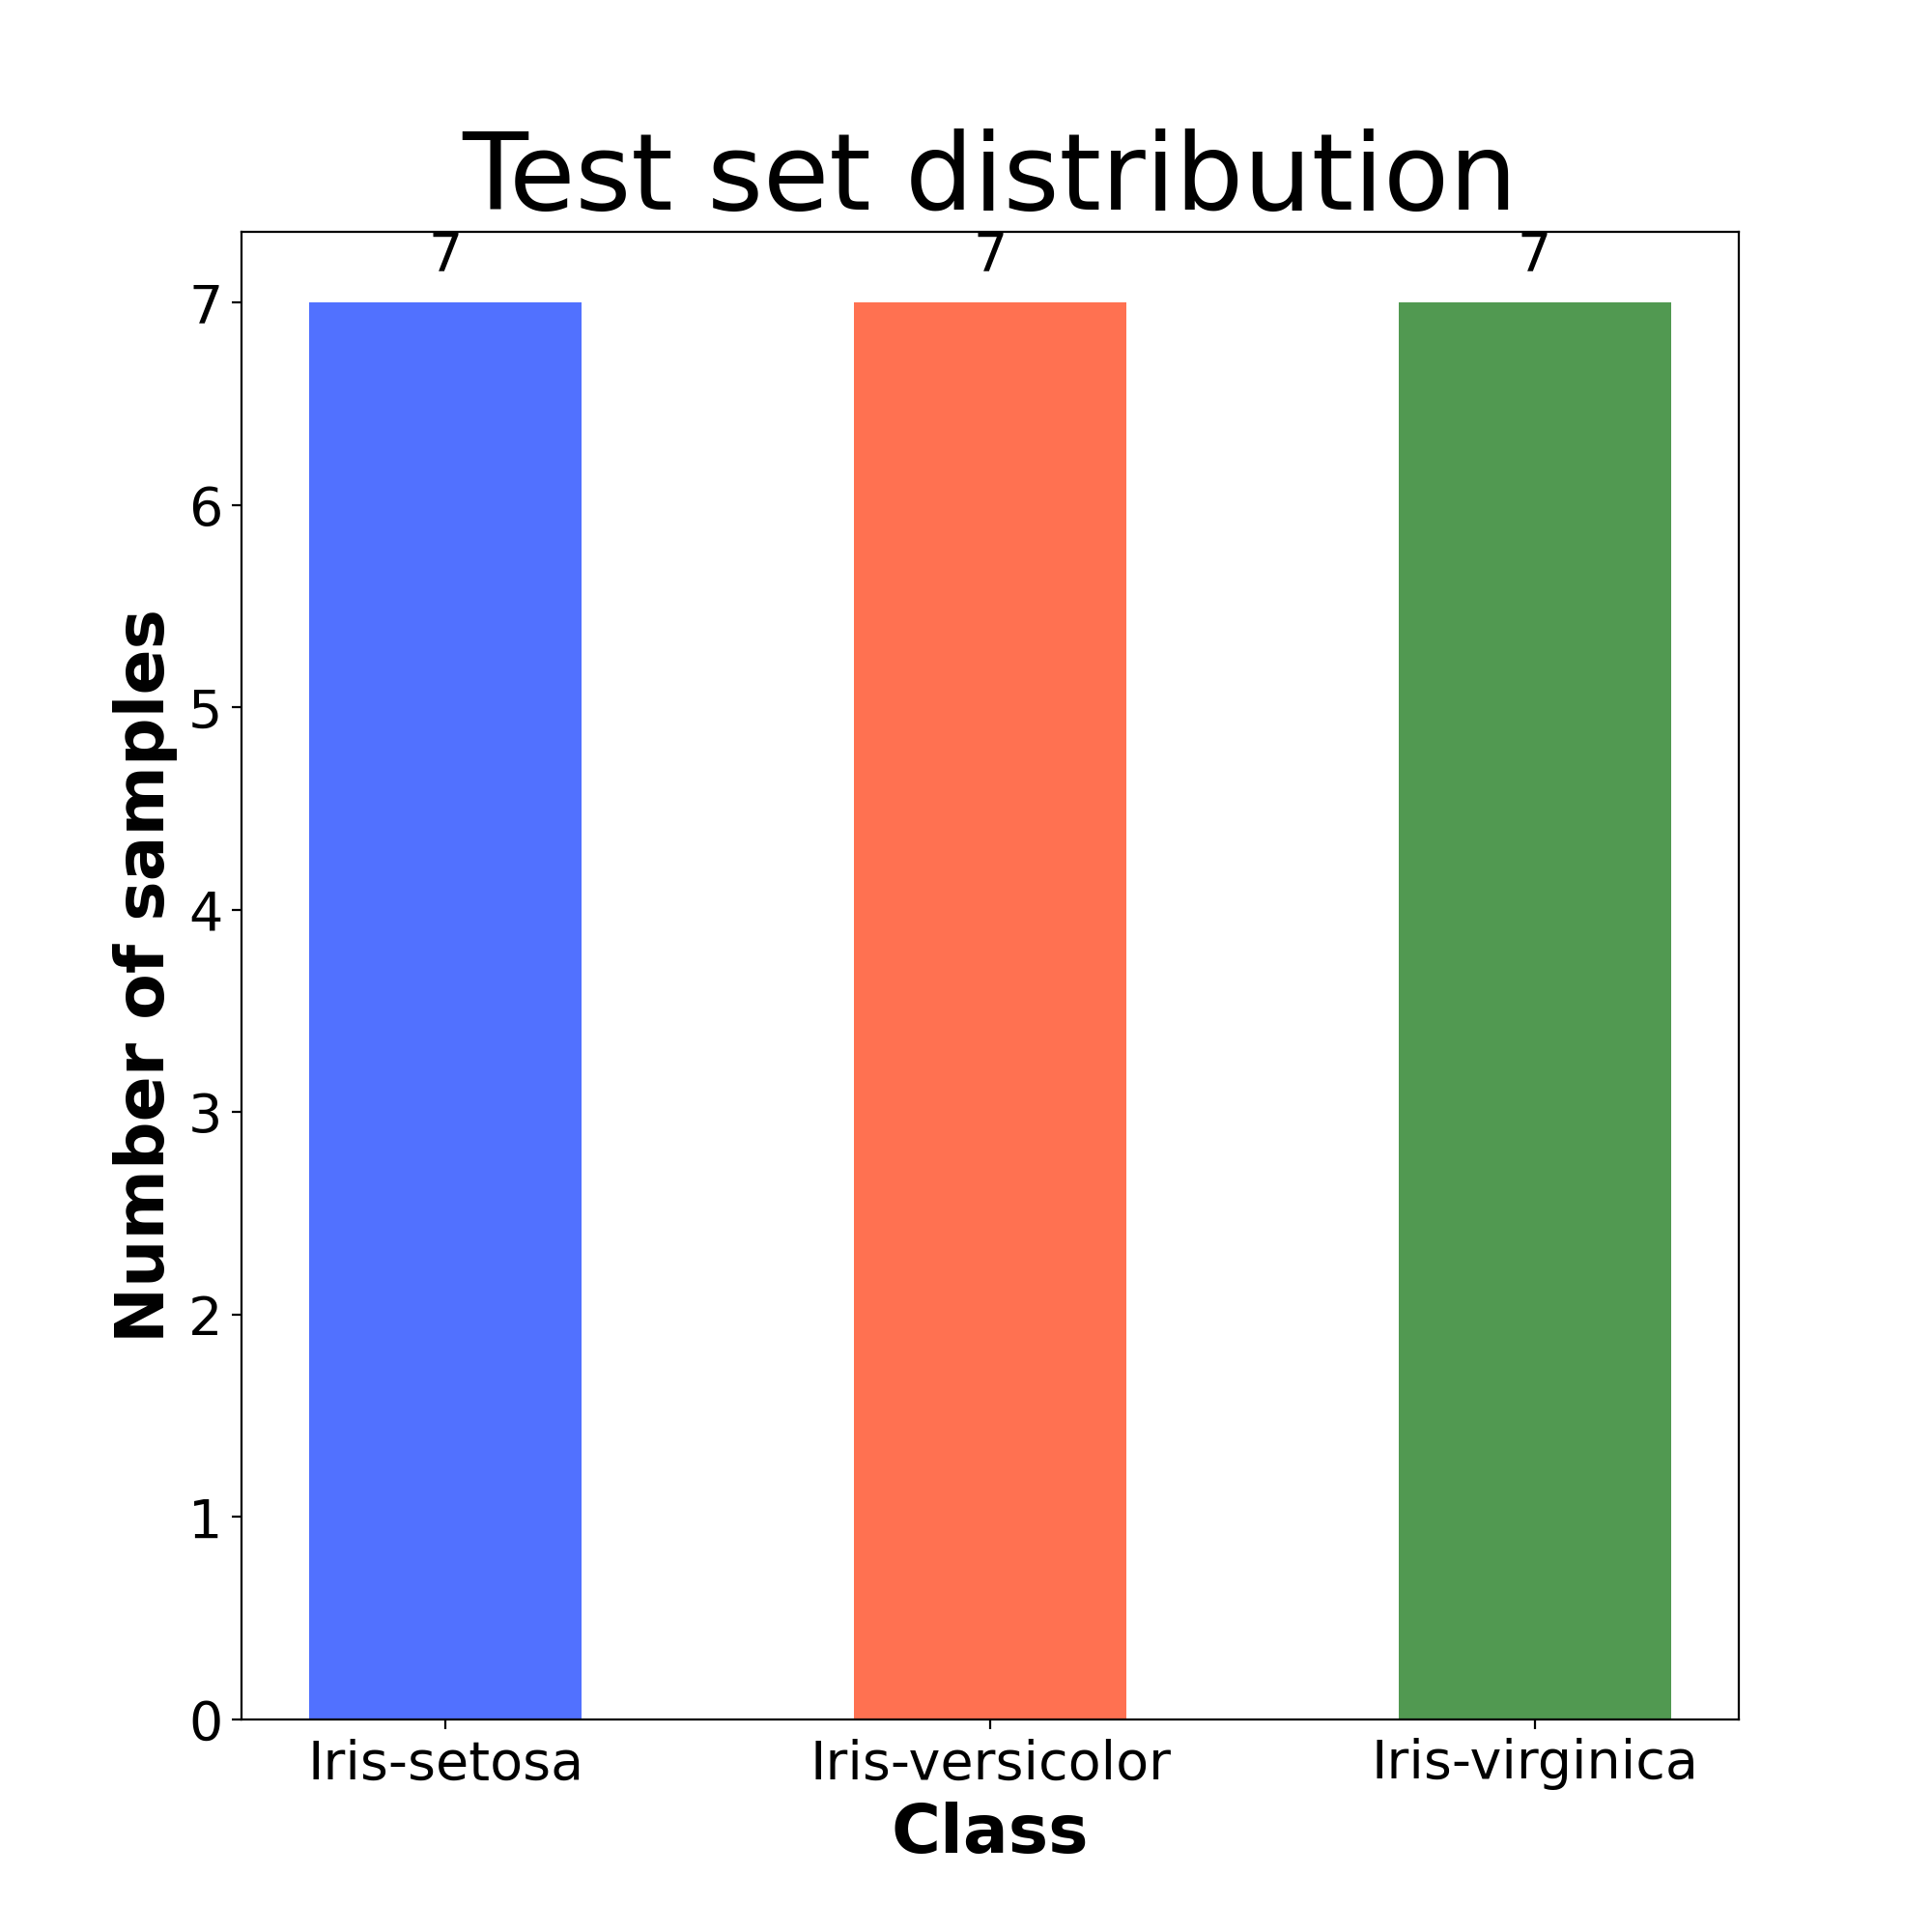
\includegraphics[width=1\textwidth]{images/exper1/iris/test_dist.png}
        \caption{Test set}
    \end{subfigure}
    \caption{\textit{Iris} balanced dataset sample distribution.}
\end{figure}

\begin{figure}[H]
    \centering % <-- added
\begin{subfigure}{0.3\textwidth}
  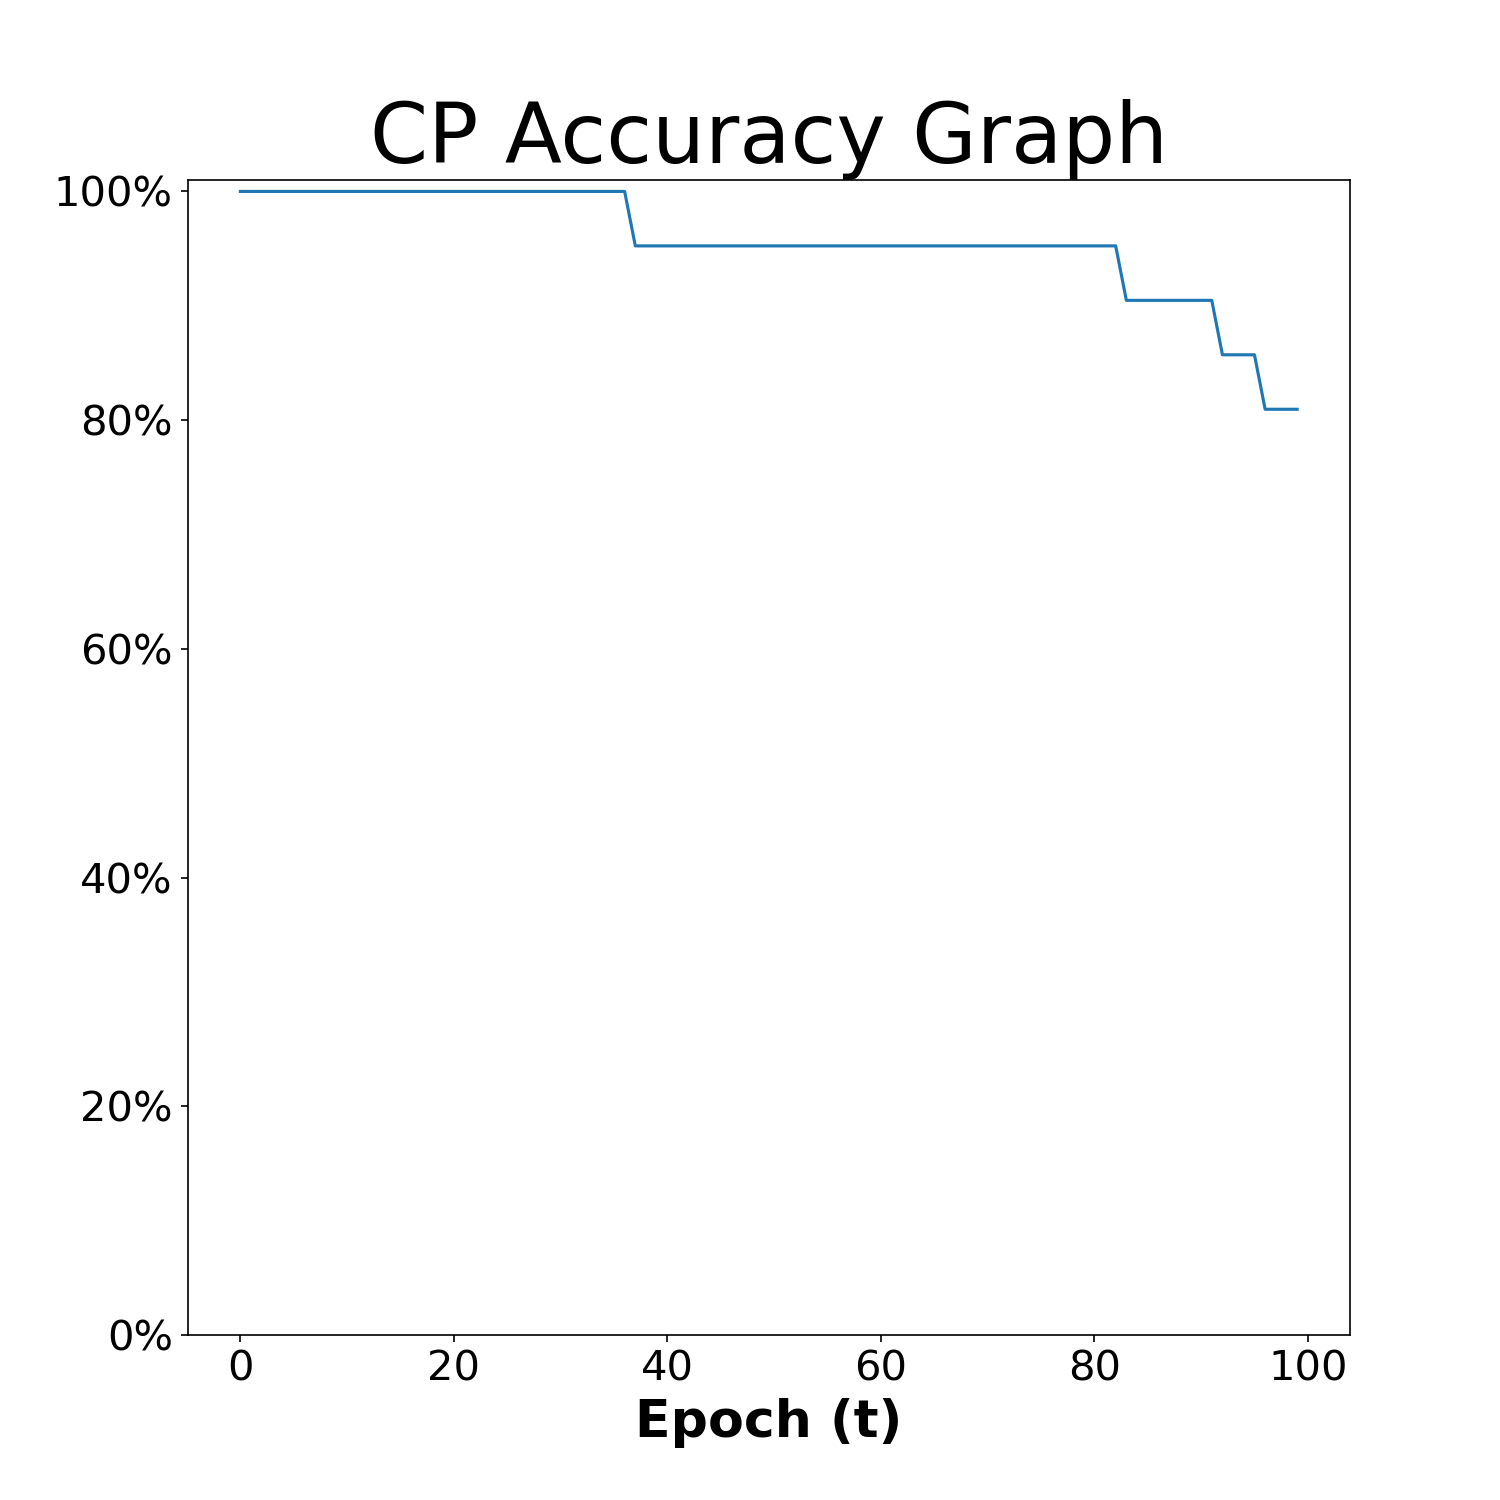
\includegraphics[width=\linewidth]{images/exper1/iris/CP_0.01_acc.png}
    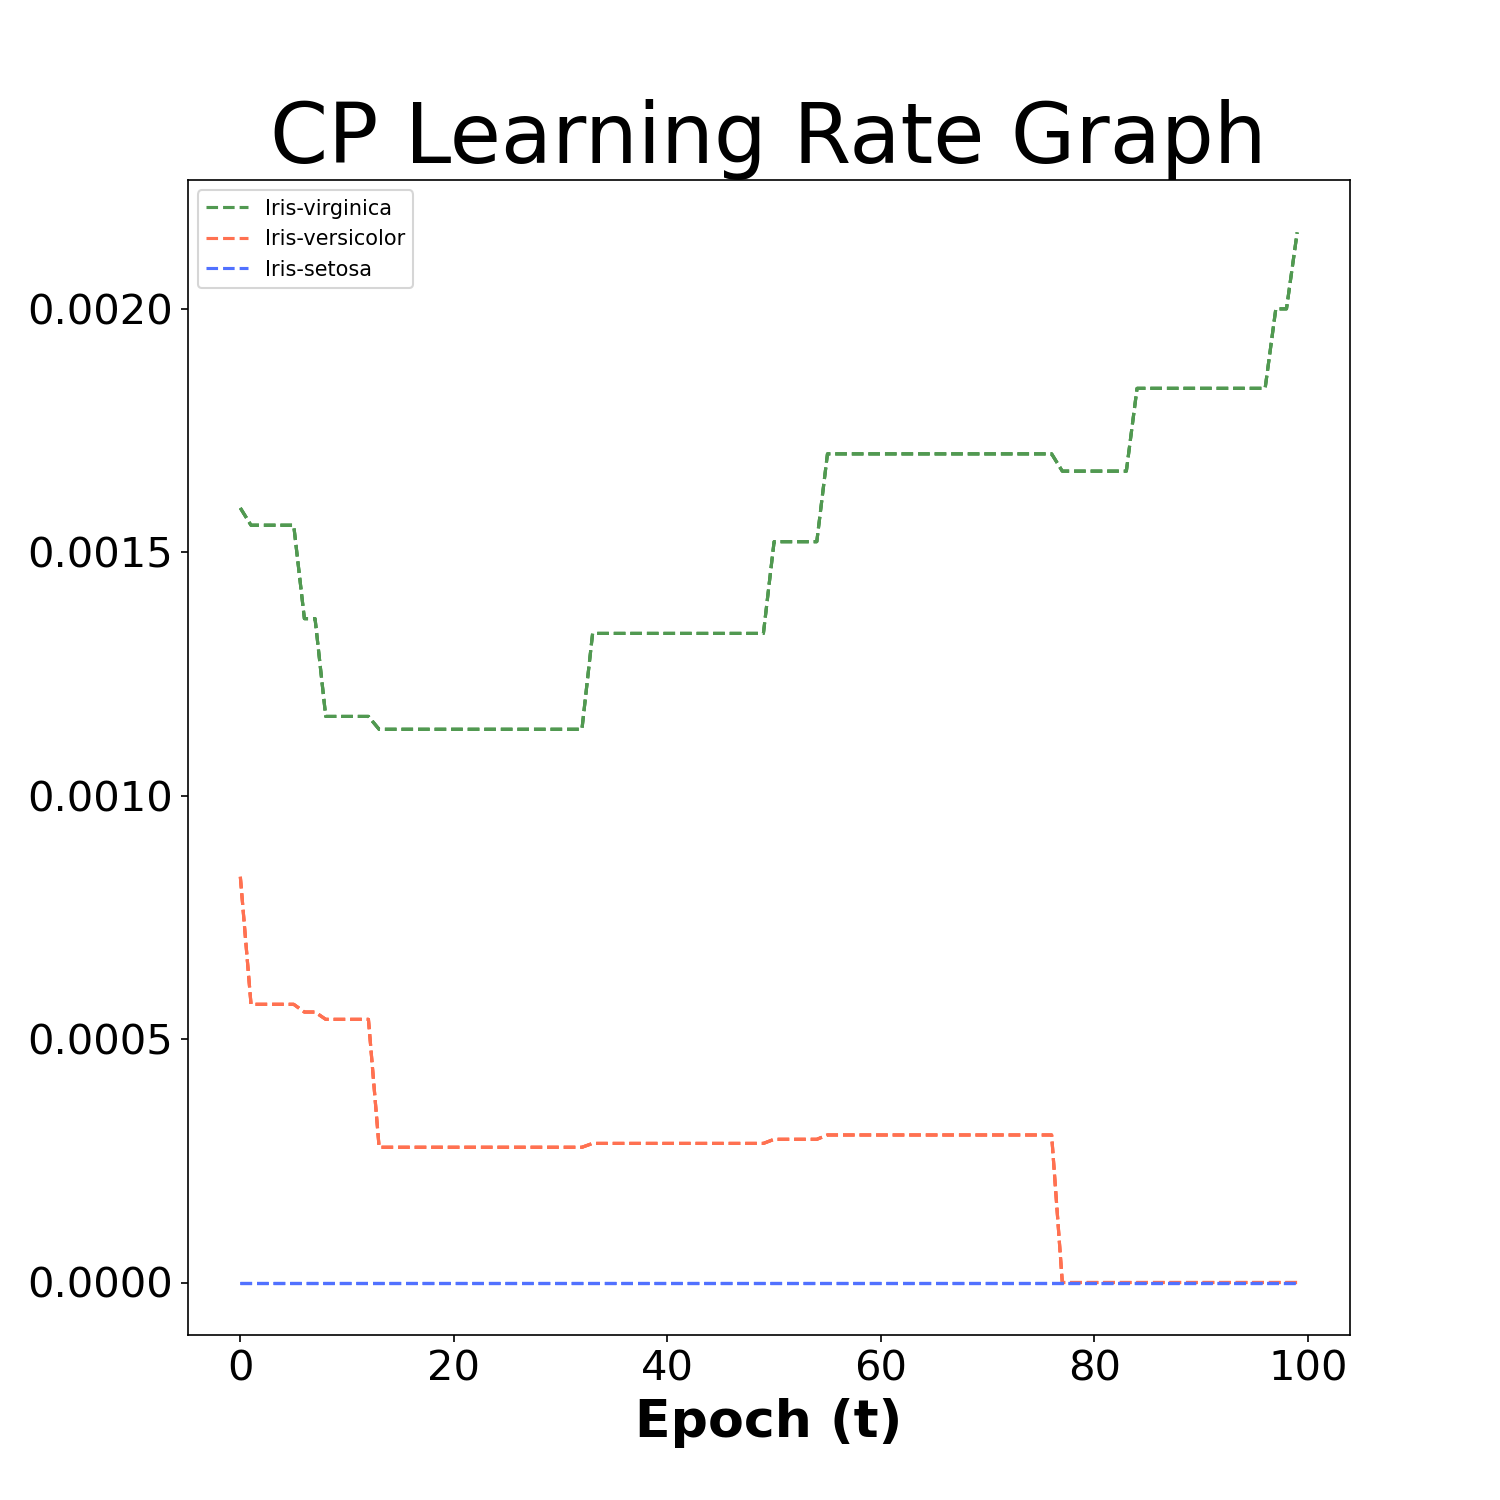
\includegraphics[width=\linewidth]{images/exper1/iris/CP_0.01_lr.png}
  \caption{$\epsilon(0)=0.01$}
\end{subfigure}\hfil % <-- added
\begin{subfigure}{0.3\textwidth}
  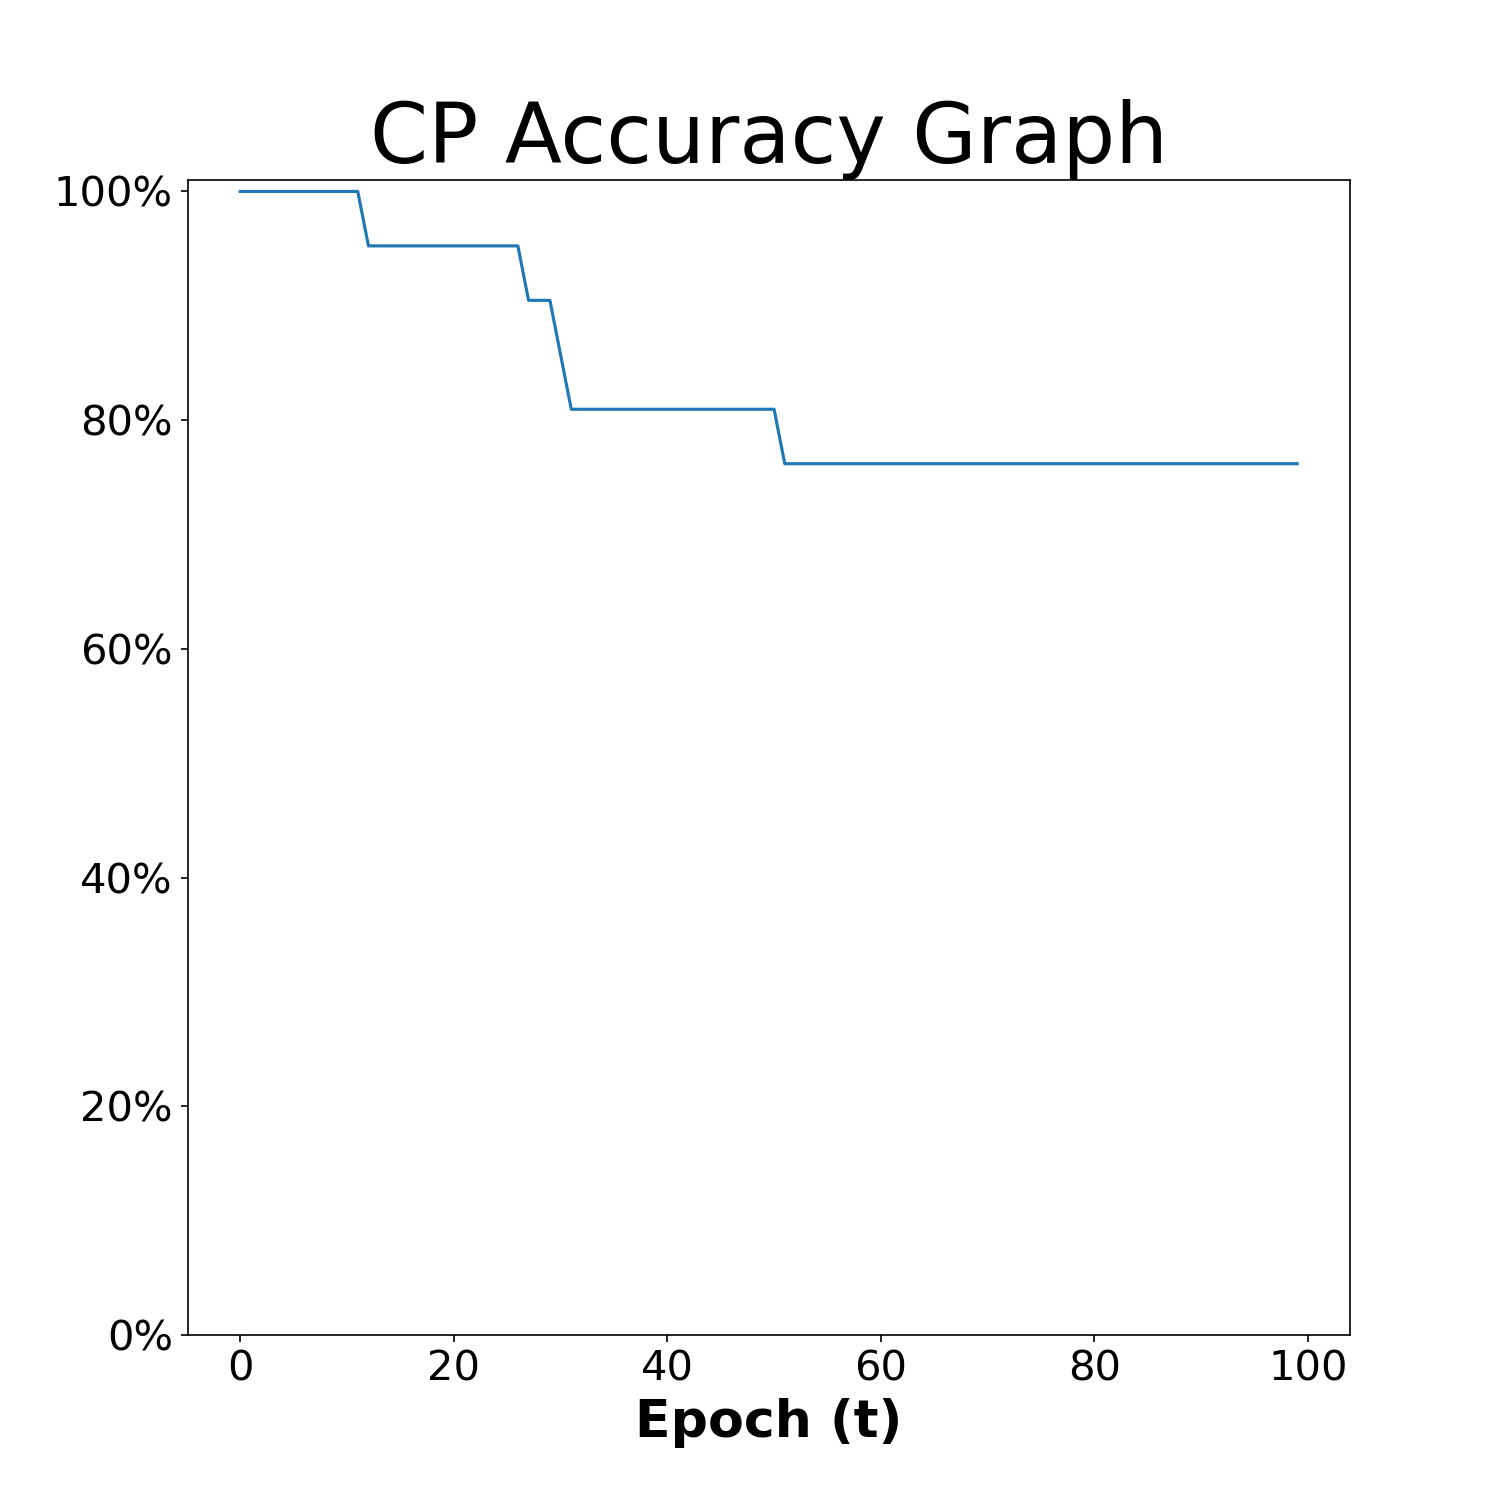
\includegraphics[width=\linewidth]{images/exper1/iris/CP_0.03_acc.png}
  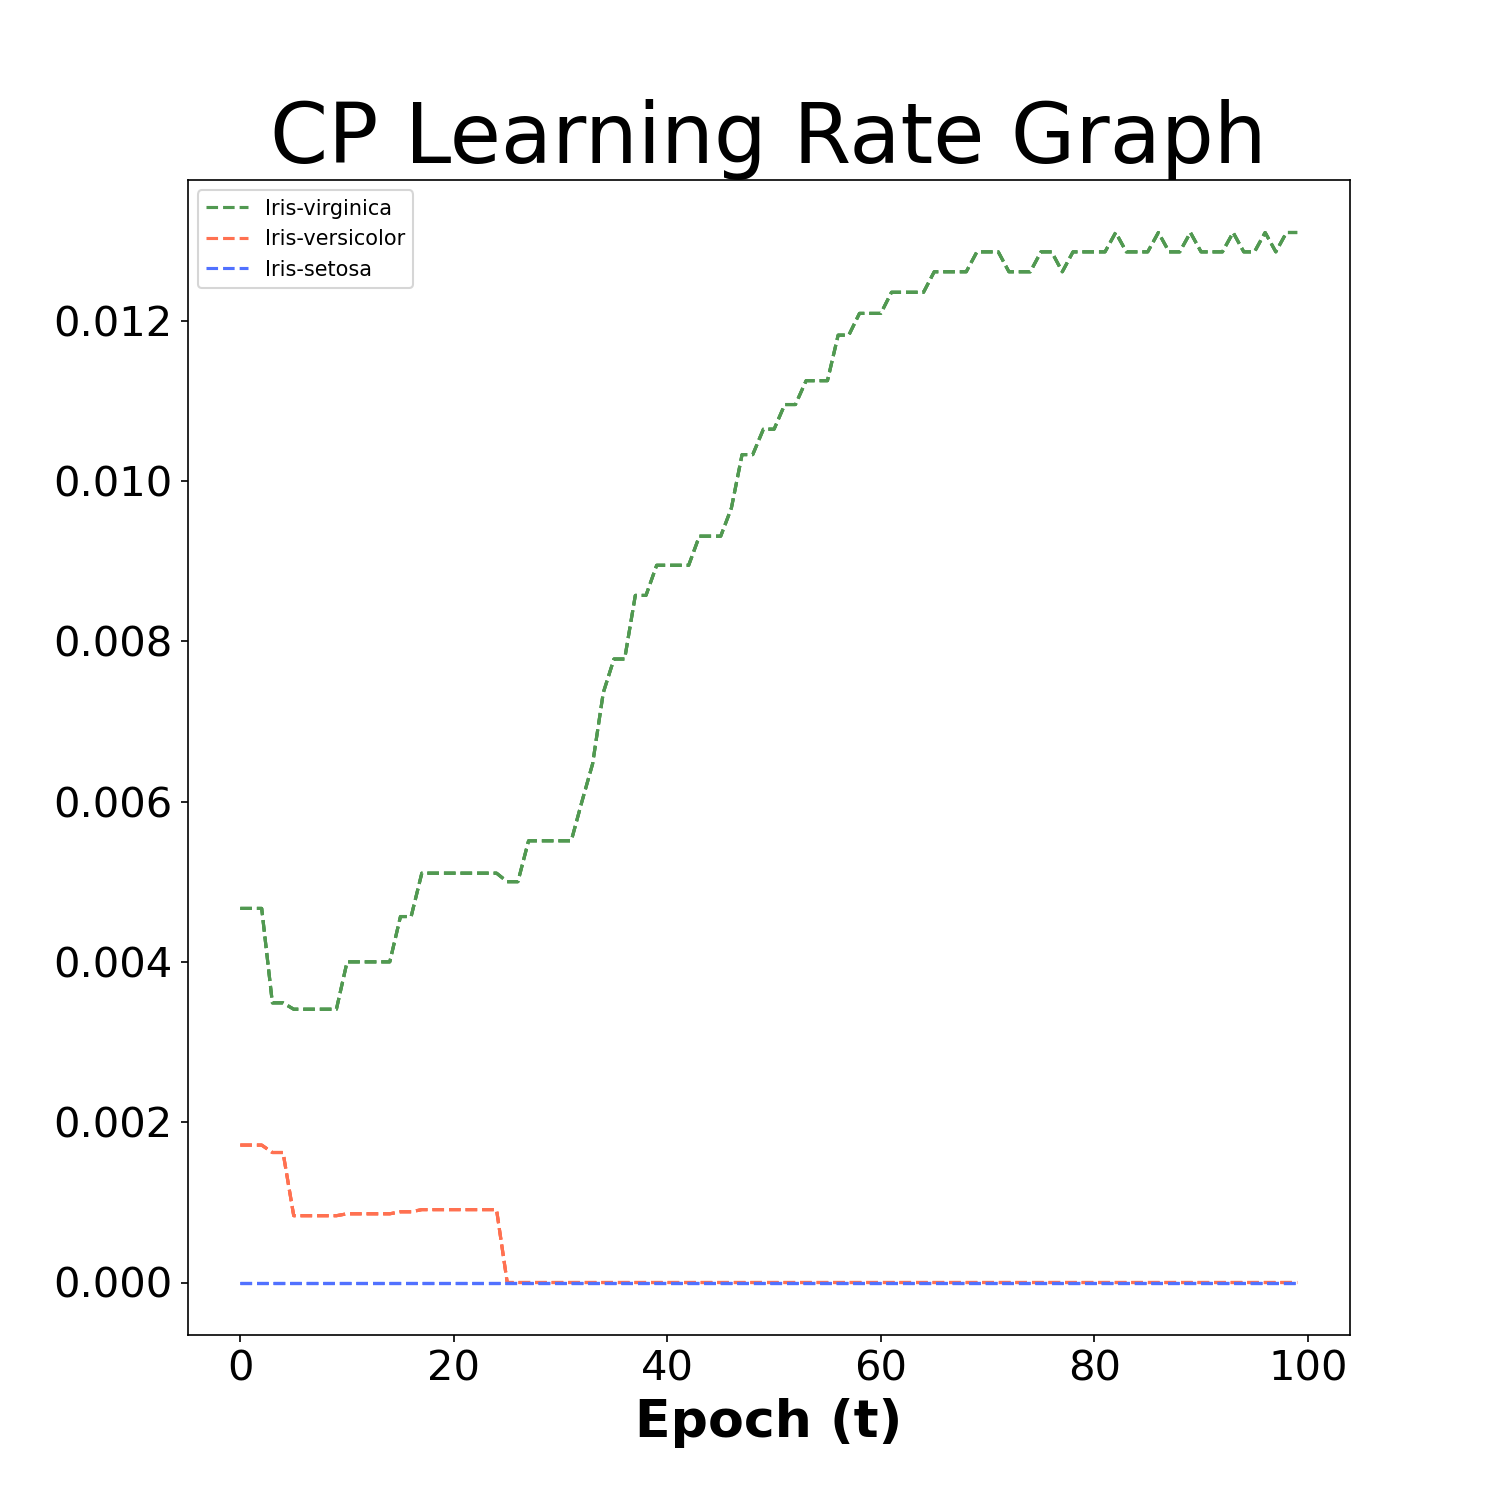
\includegraphics[width=\linewidth]{images/exper1/iris/CP_0.03_lr.png}
  \caption{$\epsilon(0)=0.03$}
\end{subfigure}\hfil % <-- added
\begin{subfigure}{0.3\textwidth}
  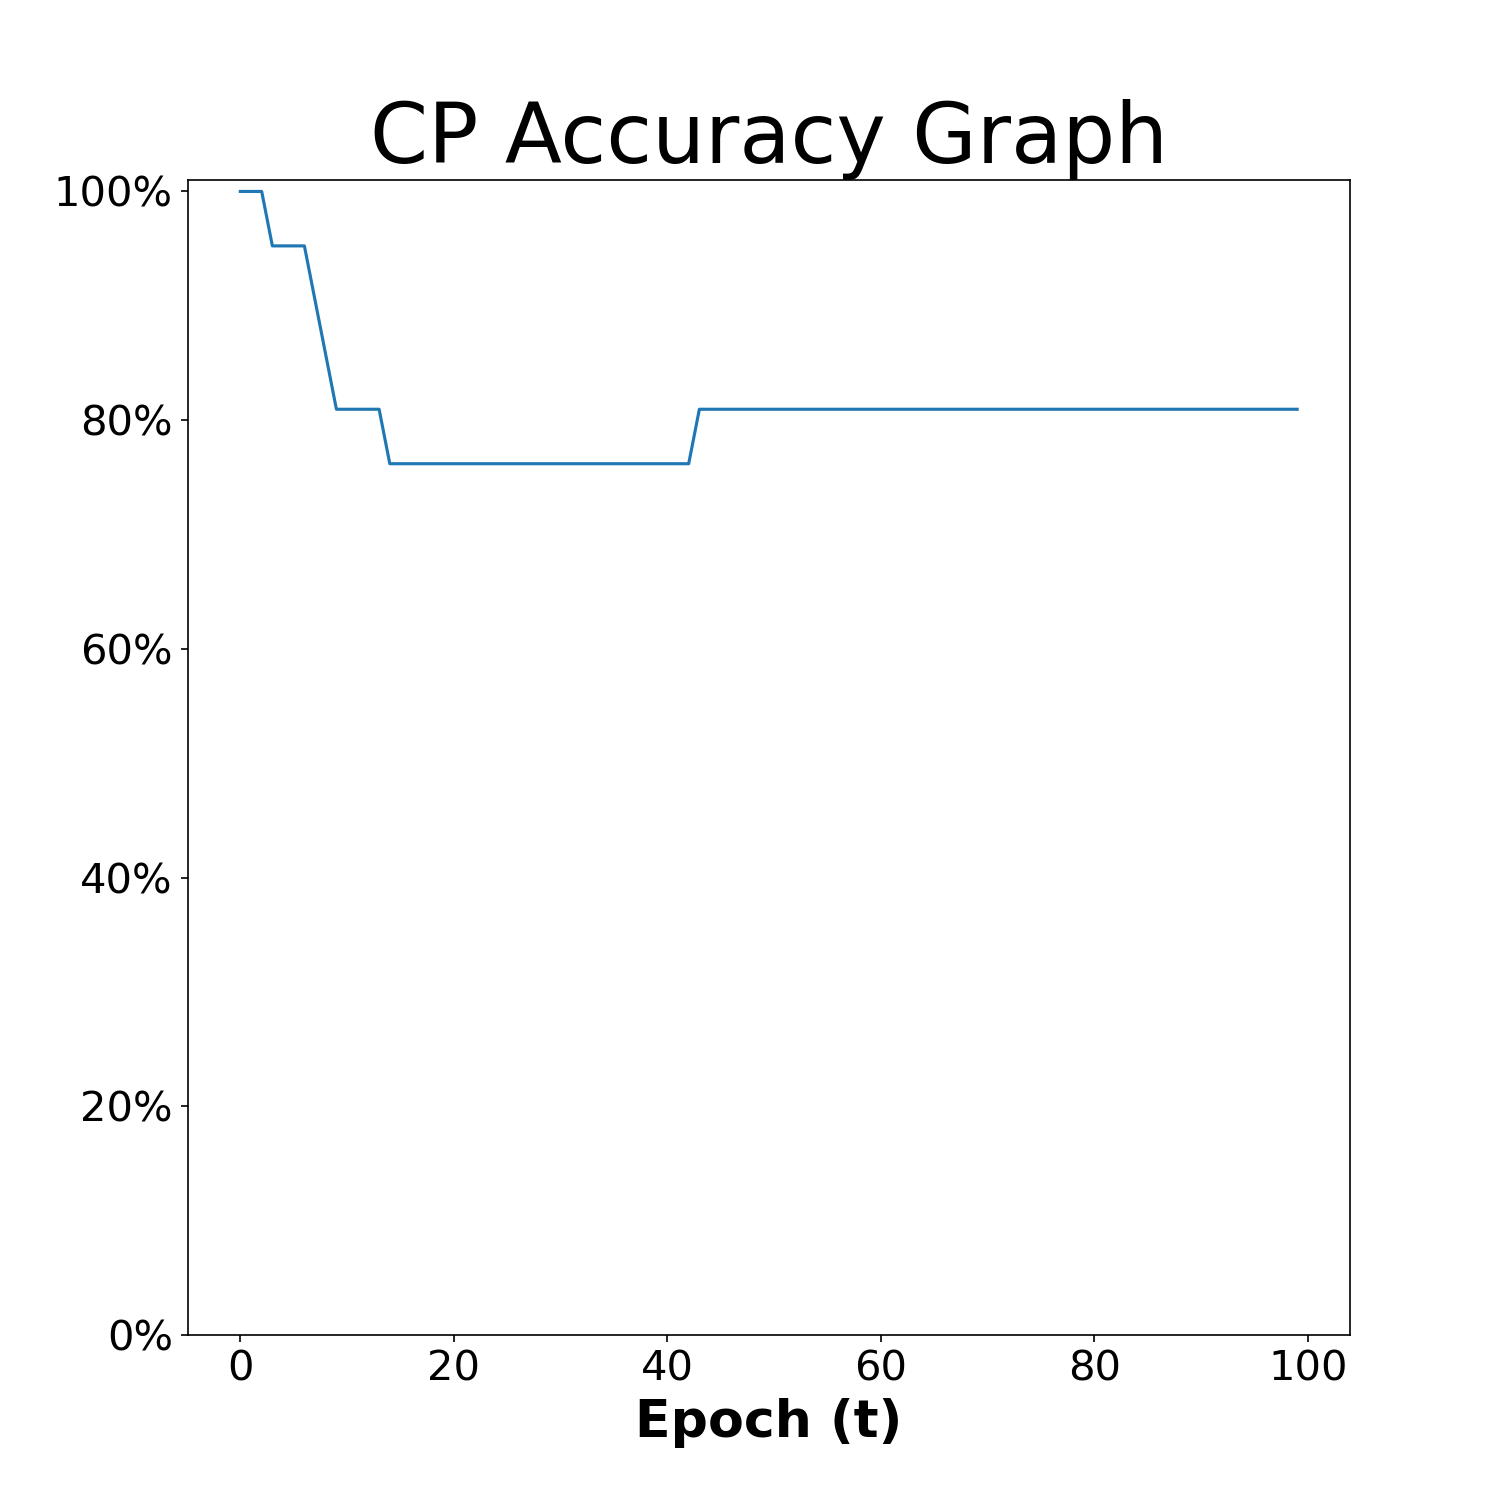
\includegraphics[width=\linewidth]{images/exper1/iris/CP_0.1_acc.png}
  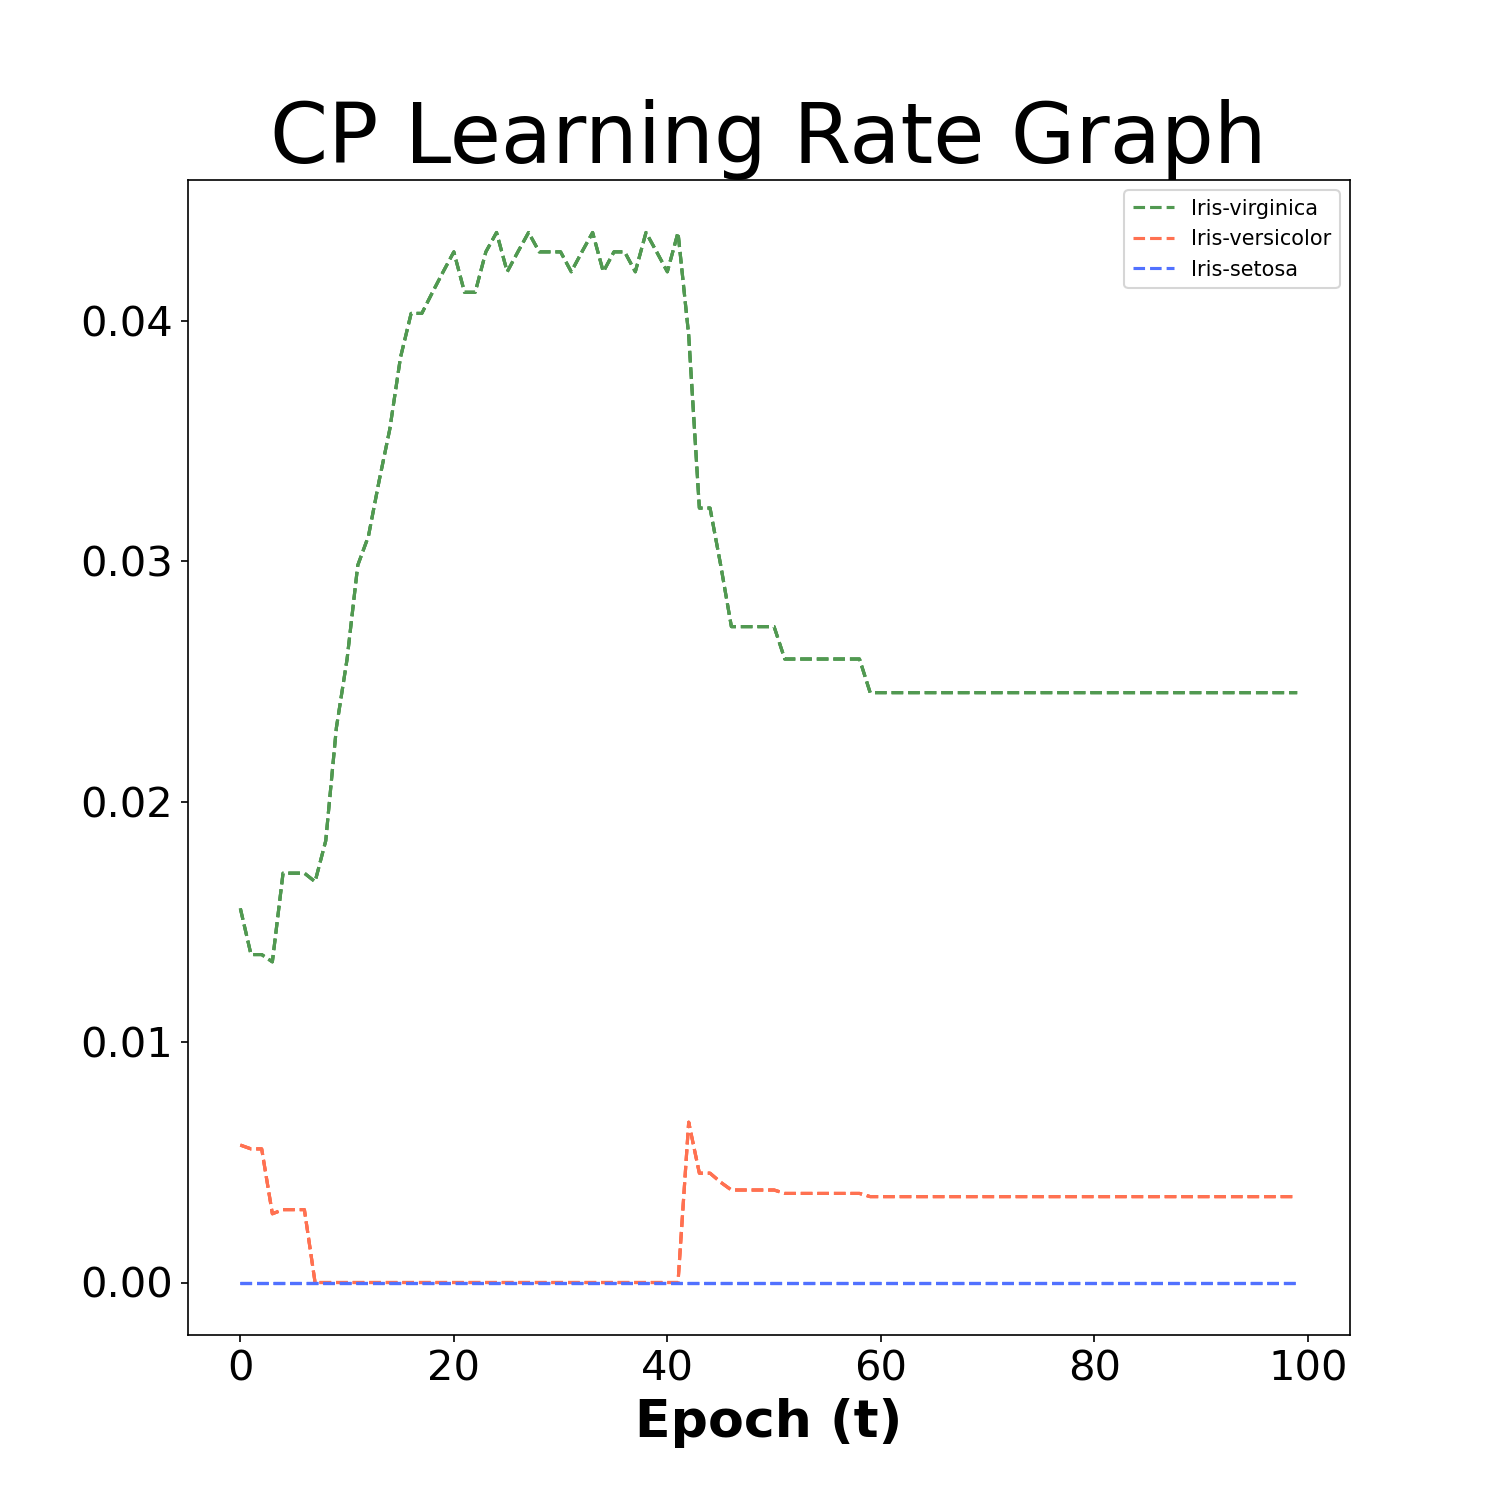
\includegraphics[width=\linewidth]{images/exper1/iris/CP_0.1_lr.png}
  \caption{$\epsilon(0)=0.1$}
\end{subfigure}

\caption{\textit{Iris} dataset accuracy score and learning rate results under CP model using balanced dataset.}
\end{figure}

\begin{figure}[H]
    \centering % <-- added
\begin{subfigure}{0.3\textwidth}
  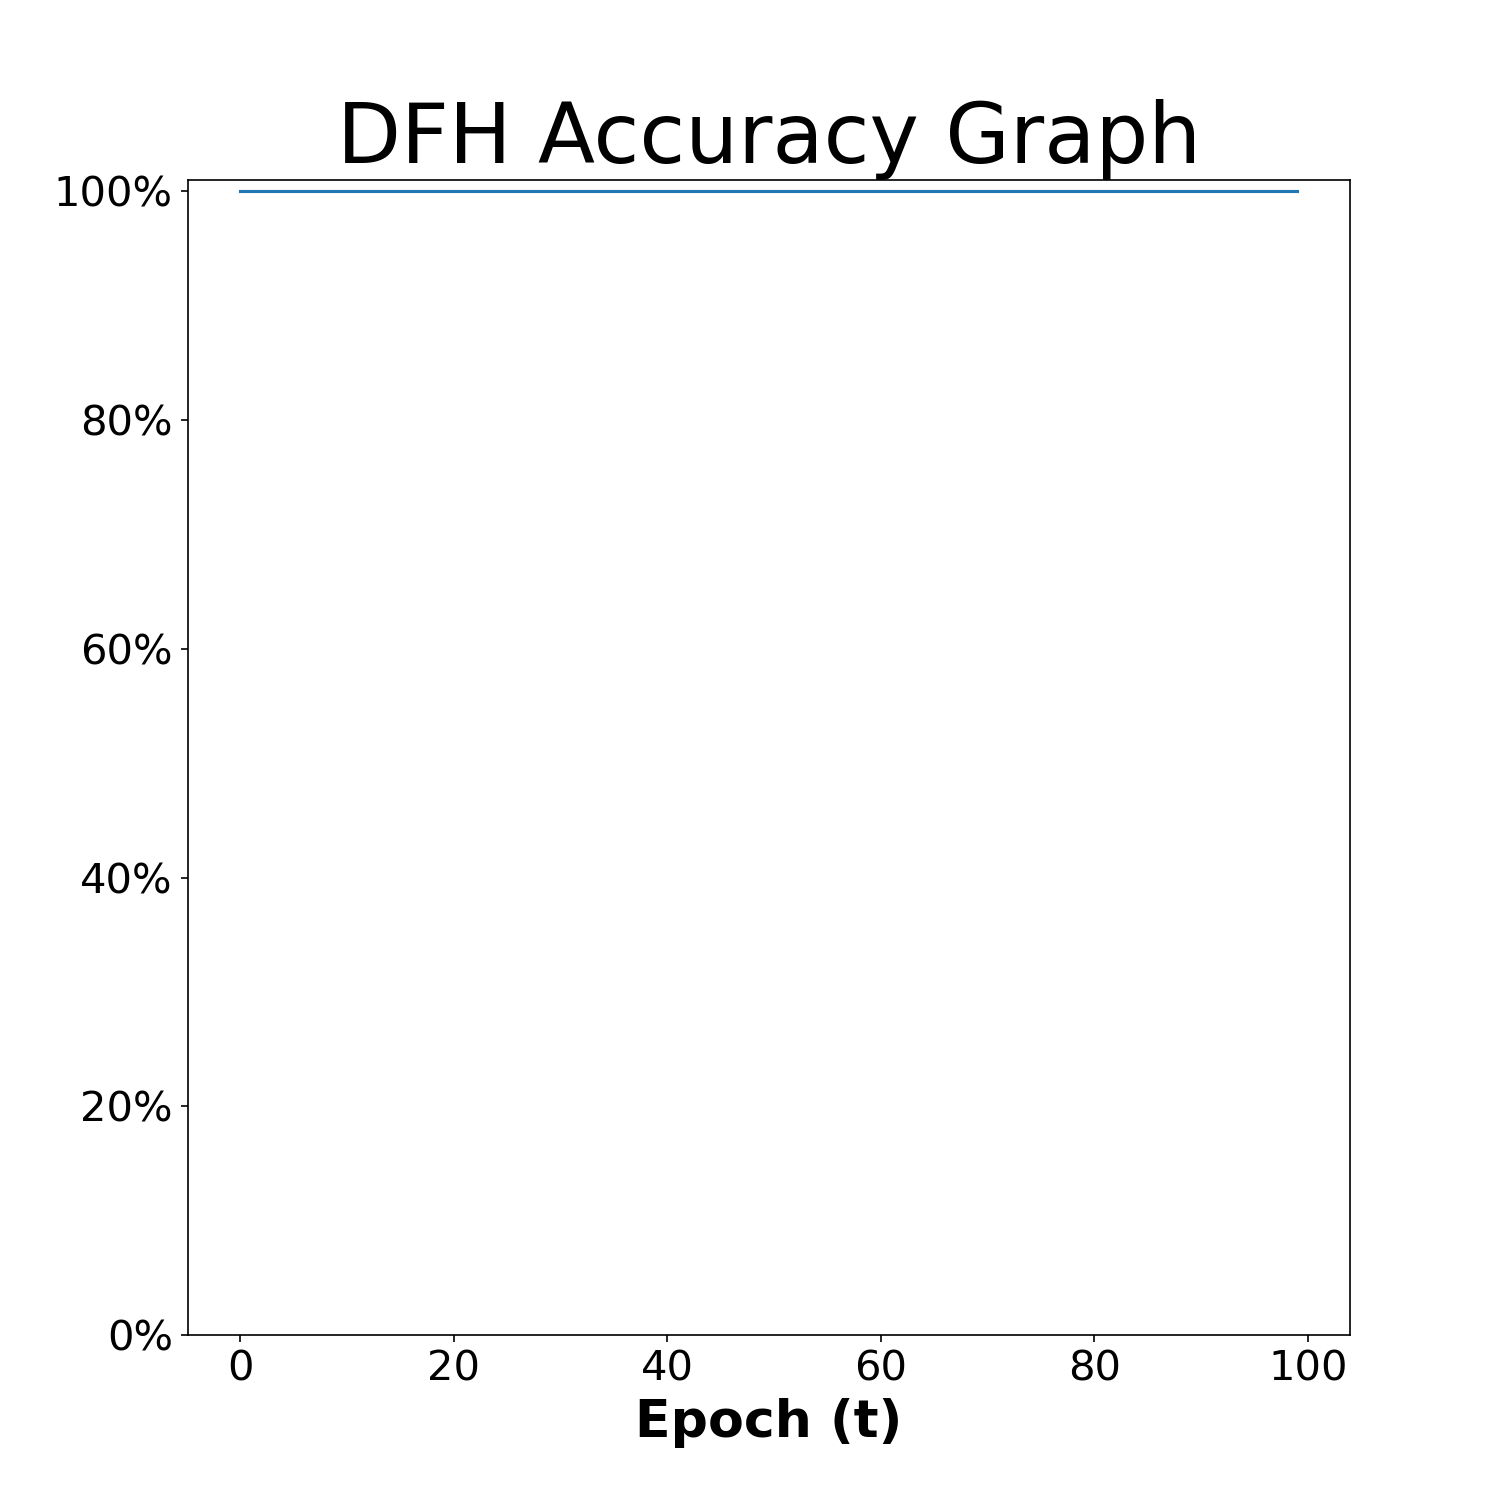
\includegraphics[width=\linewidth]{images/exper1/iris/DFH_0.01_acc.png}
    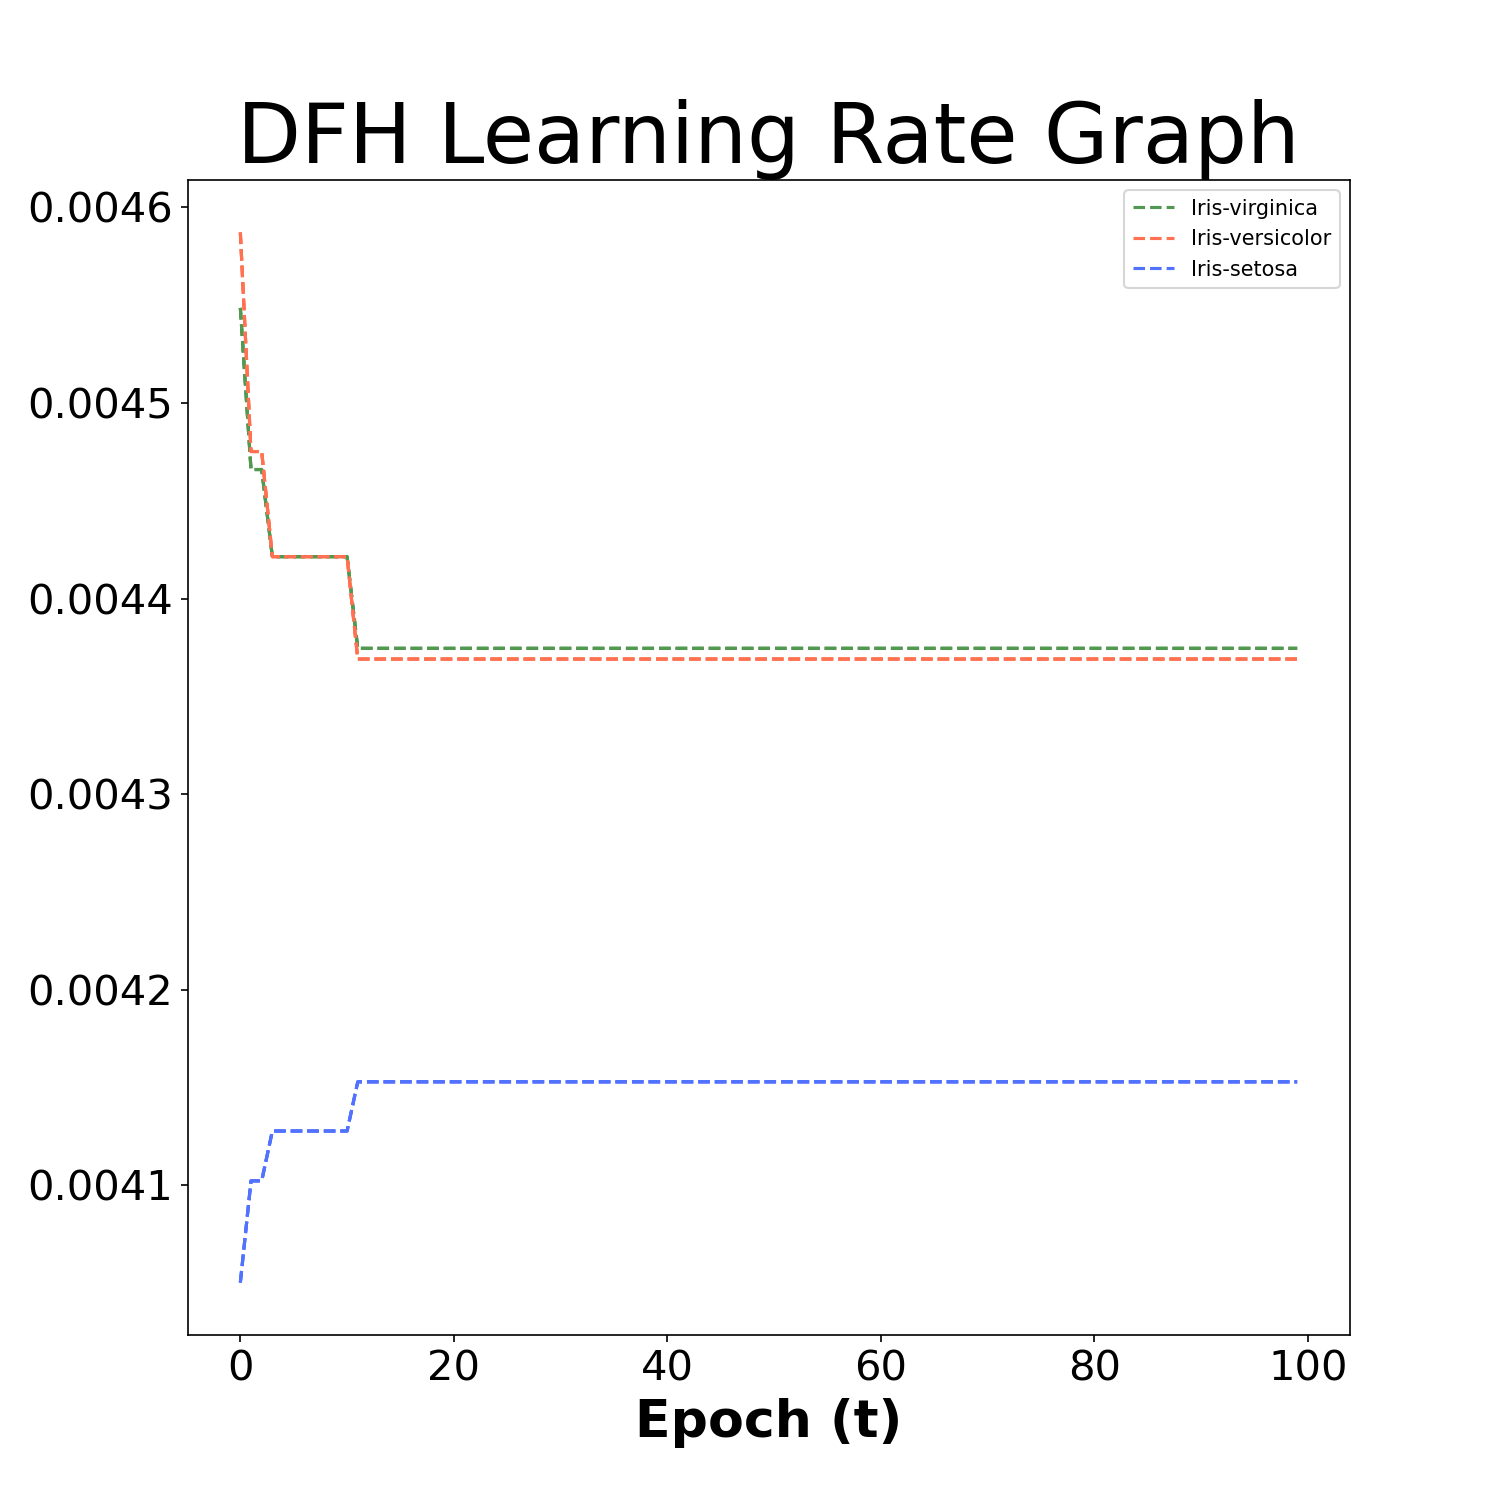
\includegraphics[width=\linewidth]{images/exper1/iris/DFH_0.01_lr.png}
  \caption{$\epsilon(0)=0.01$}
\end{subfigure}\hfil % <-- added
\begin{subfigure}{0.3\textwidth}
  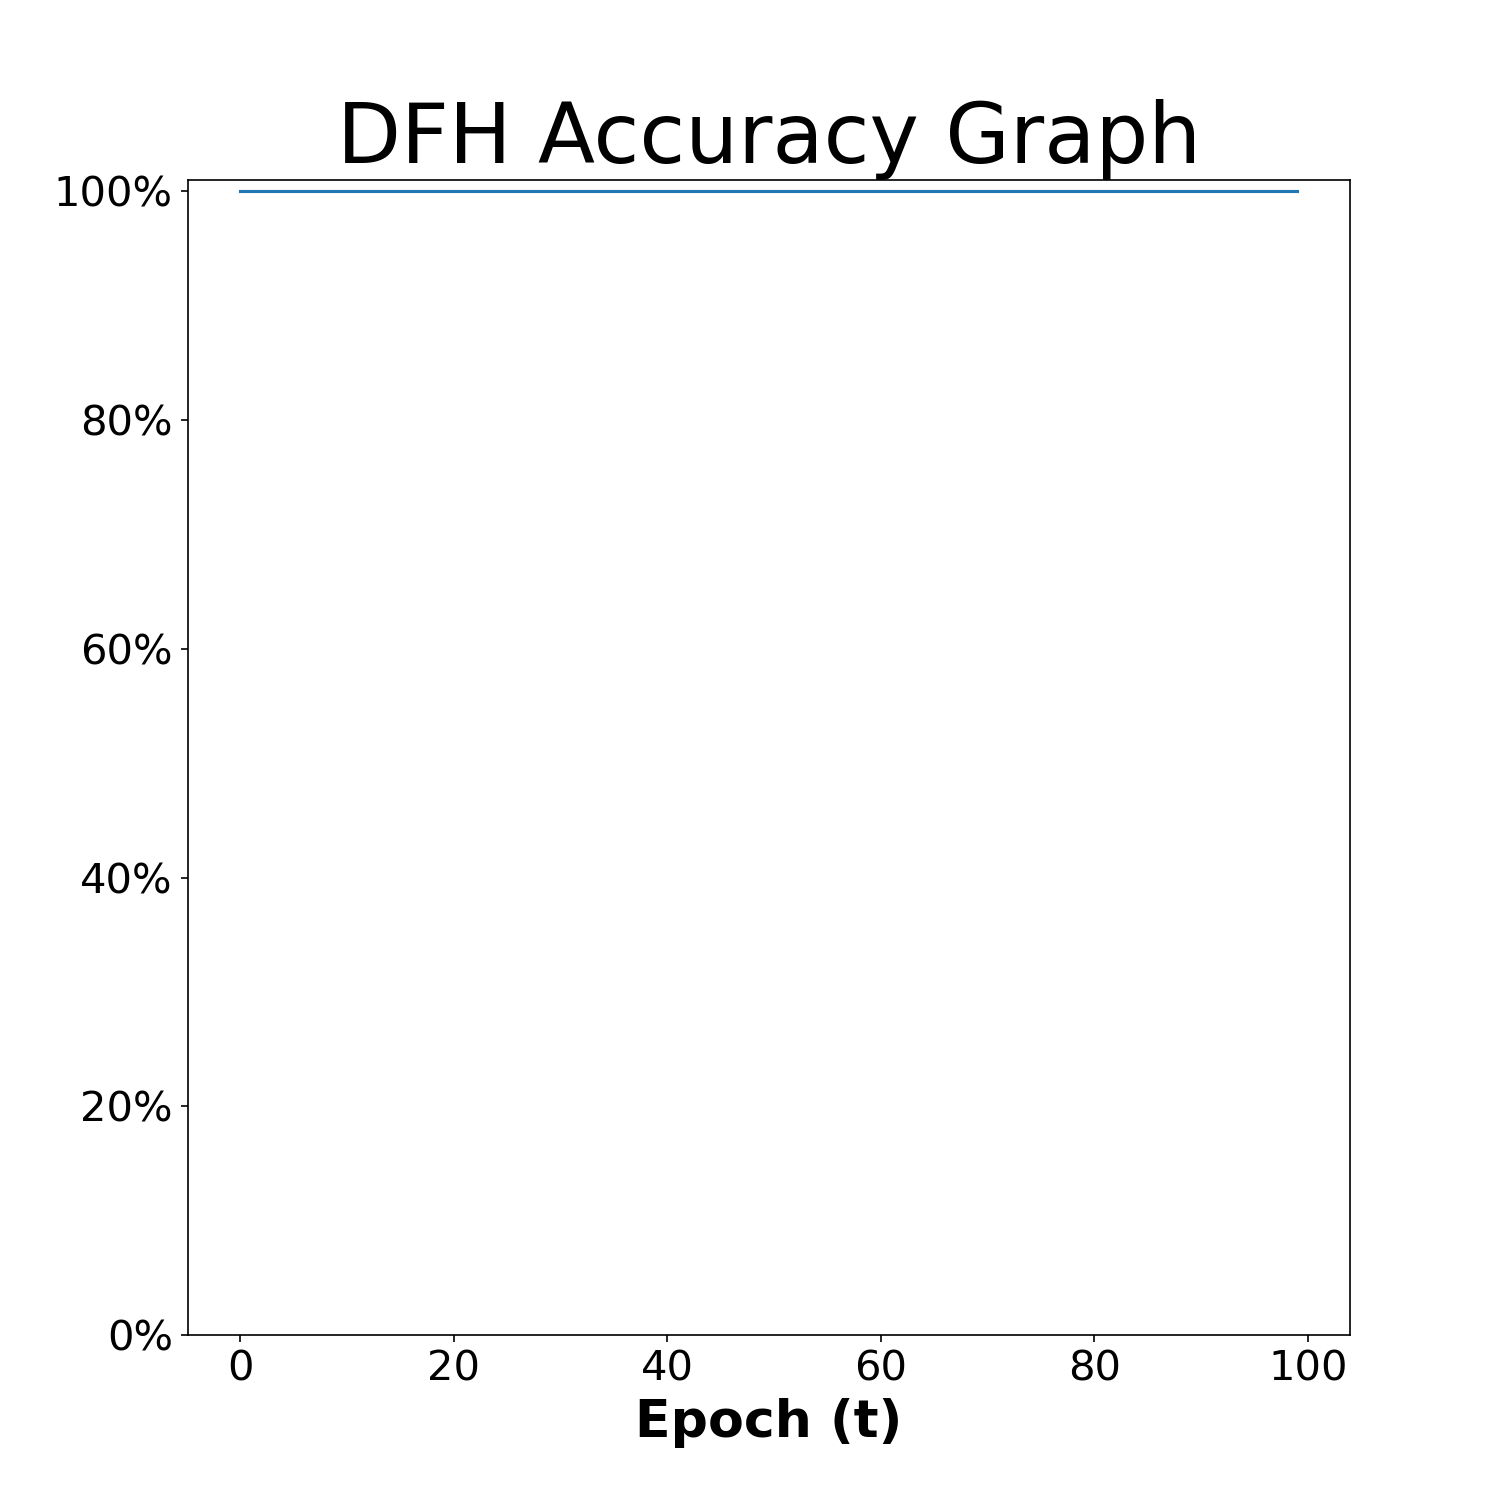
\includegraphics[width=\linewidth]{images/exper1/iris/DFH_0.03_acc.png}
  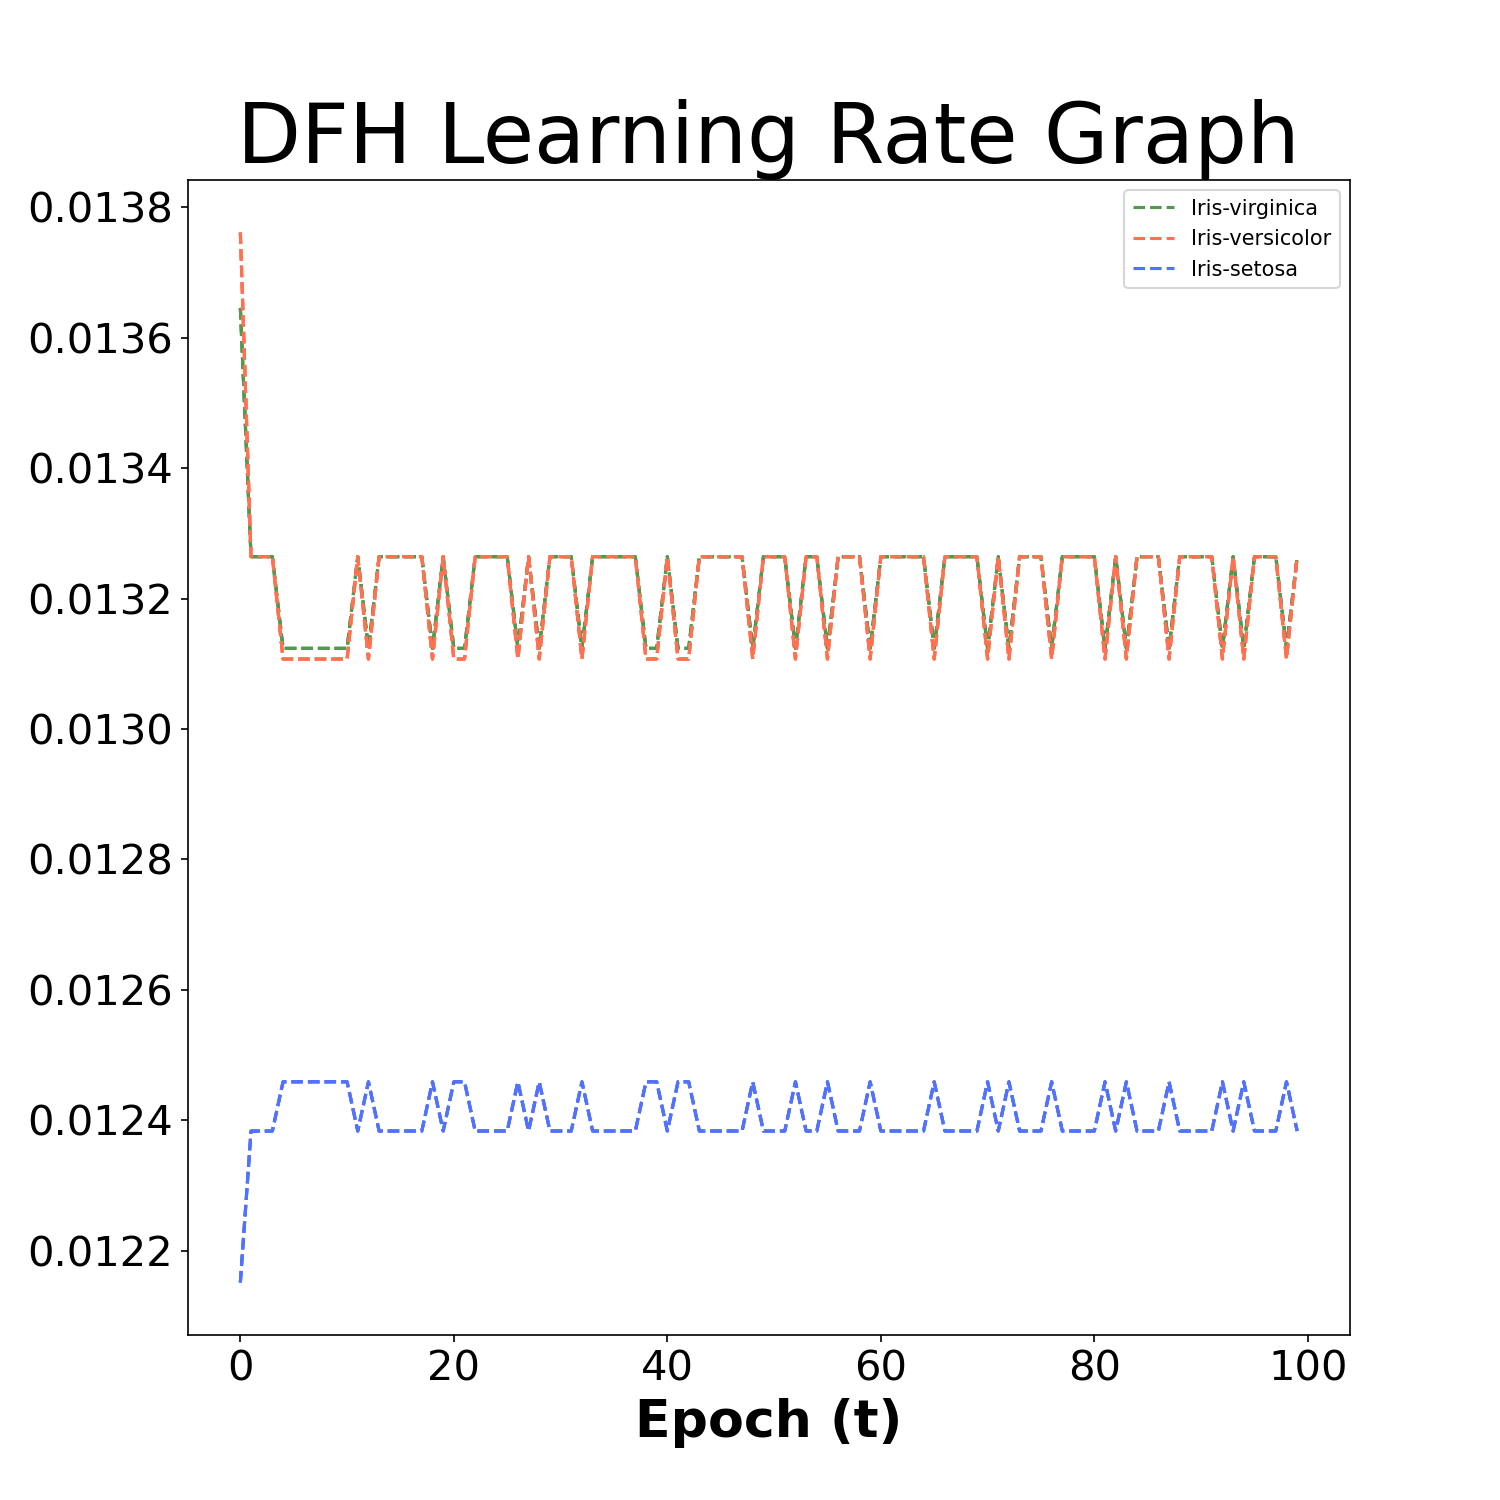
\includegraphics[width=\linewidth]{images/exper1/iris/DFH_0.03_lr.png}
  \caption{$\epsilon(0)=0.03$}
\end{subfigure}\hfil % <-- added
\begin{subfigure}{0.3\textwidth}
  \includegraphics[width=\linewidth]{images/exper1/iris/DFH_0.1_acc.png}
  \includegraphics[width=\linewidth]{images/exper1/iris/DFH_0.1_lr.png}
  \caption{$\epsilon(0)=0.1$}
\end{subfigure}

\caption{\textit{Iris} dataset accuracy score and learning rate results under DFH model using balanced dataset using balanced dataset.}
\end{figure}

\begin{figure}[H]
    \centering % <-- added
\begin{subfigure}{0.3\textwidth}
  \includegraphics[width=\linewidth]{images/exper1/iris/MS_0.01_acc.png}
    \includegraphics[width=\linewidth]{images/exper1/iris/MS_0.01_lr.png}
  \caption{$\epsilon(0)=0.01$}
\end{subfigure}\hfil % <-- added
\begin{subfigure}{0.3\textwidth}
  \includegraphics[width=\linewidth]{images/exper1/iris/MS_0.03_acc.png}
  \includegraphics[width=\linewidth]{images/exper1/iris/MS_0.03_lr.png}
  \caption{$\epsilon(0)=0.03$}
\end{subfigure}\hfil % <-- added
\begin{subfigure}{0.3\textwidth}
  \includegraphics[width=\linewidth]{images/exper1/iris/MS_0.1_acc.png}
  \includegraphics[width=\linewidth]{images/exper1/iris/MS_0.1_lr.png}
  \caption{$\epsilon(0)=0.1$}
\end{subfigure}

\caption{\textit{Iris} dataset accuracy score and learning rate results under MS model using balanced dataset.}
\end{figure}

\begin{figure}[H]
    \centering % <-- added
\begin{subfigure}{0.3\textwidth}
  \includegraphics[width=\linewidth]{images/exper1/iris/LS_0.01_acc.png}
    \includegraphics[width=\linewidth]{images/exper1/iris/LS_0.01_lr.png}
  \caption{$\epsilon(0)=0.01$}
\end{subfigure}\hfil % <-- added
\begin{subfigure}{0.3\textwidth}
  \includegraphics[width=\linewidth]{images/exper1/iris/LS_0.03_acc.png}
  \includegraphics[width=\linewidth]{images/exper1/iris/LS_0.03_lr.png}
  \caption{$\epsilon(0)=0.03$}
\end{subfigure}\hfil % <-- added
\begin{subfigure}{0.3\textwidth}
  \includegraphics[width=\linewidth]{images/exper1/iris/LS_0.1_acc.png}
  \includegraphics[width=\linewidth]{images/exper1/iris/LS_0.1_lr.png}
  \caption{$\epsilon(0)=0.1$}
\end{subfigure}

\caption{\textit{Iris} dataset accuracy score and learning rate results under LS model using balanced dataset.}
\end{figure}

\begin{figure}[H]
    \centering % <-- added
\begin{subfigure}{0.3\textwidth}
  \includegraphics[width=\linewidth]{images/exper1/iris/LSR_0.01_acc.png}
    \includegraphics[width=\linewidth]{images/exper1/iris/LSR_0.01_lr.png}
  \caption{$\epsilon(0)=0.01$}
\end{subfigure}\hfil % <-- added
\begin{subfigure}{0.3\textwidth}
  \includegraphics[width=\linewidth]{images/exper1/iris/LSR_0.03_acc.png}
  \includegraphics[width=\linewidth]{images/exper1/iris/LSR_0.03_lr.png}
  \caption{$\epsilon(0)=0.03$}
\end{subfigure}\hfil % <-- added
\begin{subfigure}{0.3\textwidth}
  \includegraphics[width=\linewidth]{images/exper1/iris/LSR_0.1_acc.png}
  \includegraphics[width=\linewidth]{images/exper1/iris/LSR_0.1_lr.png}
  \caption{$\epsilon(0)=0.1$}
\end{subfigure}

\caption{\textit{Iris} dataset accuracy score and learning rate results under LSR model using balanced dataset.}
\end{figure}

\begin{figure}[H]
    \centering % <-- added
\begin{subfigure}{0.3\textwidth}
  \includegraphics[width=\linewidth]{images/exper1/iris/OGLVQ_0.01_acc.png}
    \includegraphics[width=\linewidth]{images/exper1/iris/OGLVQ_0.01_lr.png}
  \caption{$\epsilon(0)=0.01$}
\end{subfigure}\hfil % <-- added
\begin{subfigure}{0.3\textwidth}
  \includegraphics[width=\linewidth]{images/exper1/iris/OGLVQ_0.03_acc.png}
  \includegraphics[width=\linewidth]{images/exper1/iris/OGLVQ_0.03_lr.png}
  \caption{$\epsilon(0)=0.03$}
\end{subfigure}\hfil % <-- added
\begin{subfigure}{0.3\textwidth}
  \includegraphics[width=\linewidth]{images/exper1/iris/OGLVQ_0.1_acc.png}
  \includegraphics[width=\linewidth]{images/exper1/iris/OGLVQ_0.1_lr.png}
  \caption{$\epsilon(0)=0.1$}
\end{subfigure}

\caption{\textit{Iris} dataset accuracy score and learning rate results under OGLVQ model using balanced dataset.}
\end{figure}




\subsection{Ionosphere dataset}

Prototypes for each class: 3
\vspace{5pt}

\textit{Ionosphere} dataset results of experiment 1 for all models look promising, even though we do not have high or constantly increasing accuracy scores. All the models learn with proper $\epsilon(0)$ (CP with $\epsilon(0)$ 0.01 and 0.03, MS with $\epsilon(0)$ 0.01 and all other CGLVQ models) during their training period, as we can see by the decrease of $\epsilon_{i}$ values. The CP model with $\epsilon(0) = 0.1$ graph looks bad for learning as we can see on Figure~\ref{ioncp1} because of the increasing $\epsilon_{g}$, but $\epsilon_{g}$ curve might be the result of the high $\epsilon(0)$ since other CP models with lower $\epsilon(0)$ have a nice $\epsilon_{g}$ curves. So $\epsilon(0)= 0.1$ might be overshooting for the CP model in this case. Additionally, the OGLVQ models’ learning rate graphs do not look promising (Figure~\ref{1ionglvq}). Even if we see an increase in accuracy, learning rates of class “Bad” during the learning tends to increase or stay stable, which ends up in bad decision-making for class “Bad” with the model.



\begin{figure}[H]
    \centering
    \begin{subfigure}[t]{0.45\textwidth}
        \centering
        \includegraphics[width=1\textwidth]{images/exper1/Ionosphere/train_dist.png}
        \caption{Training set}
    \end{subfigure}
    \begin{subfigure}[t]{0.45\textwidth}
        \centering
        \includegraphics[width=1\textwidth]{images/exper1/Ionosphere/test_dist.png}
        \caption{Test set}
    \end{subfigure}
    \caption{\textit{Ionosphere} balanced dataset sample distribution.}
\end{figure}

\begin{figure}[H]
    \centering % <-- added
\begin{subfigure}{0.3\textwidth}
  \includegraphics[width=\linewidth]{images/exper1/Ionosphere/CP_0.01_acc.png}
    \includegraphics[width=\linewidth]{images/exper1/Ionosphere/CP_0.01_lr.png}
  \caption{$\epsilon(0)=0.01$}
\end{subfigure}\hfil % <-- added
\begin{subfigure}{0.3\textwidth}
  \includegraphics[width=\linewidth]{images/exper1/Ionosphere/CP_0.03_acc.png}
  \includegraphics[width=\linewidth]{images/exper1/Ionosphere/CP_0.03_lr.png}
  \caption{$\epsilon(0)=0.03$}
\end{subfigure}\hfil % <-- added
\begin{subfigure}{0.3\textwidth}
  \includegraphics[width=\linewidth]{images/exper1/Ionosphere/CP_0.1_acc.png}
  \includegraphics[width=\linewidth]{images/exper1/Ionosphere/CP_0.1_lr.png}
  \caption{$\epsilon(0)=0.1$}\label{ioncp1}
\end{subfigure}

\caption{\textit{Ionosphere} dataset accuracy score and learning rate results under CP model using balanced dataset.}
\end{figure}

\begin{figure}[H]
    \centering % <-- added
\begin{subfigure}{0.3\textwidth}
  \includegraphics[width=\linewidth]{images/exper1/Ionosphere/DFH_0.01_acc.png}
    \includegraphics[width=\linewidth]{images/exper1/Ionosphere/DFH_0.01_lr.png}
  \caption{$\epsilon(0)=0.01$}
\end{subfigure}\hfil % <-- added
\begin{subfigure}{0.3\textwidth}
  \includegraphics[width=\linewidth]{images/exper1/Ionosphere/DFH_0.03_acc.png}
  \includegraphics[width=\linewidth]{images/exper1/Ionosphere/DFH_0.03_lr.png}
  \caption{$\epsilon(0)=0.03$}
\end{subfigure}\hfil % <-- added
\begin{subfigure}{0.3\textwidth}
  \includegraphics[width=\linewidth]{images/exper1/Ionosphere/DFH_0.1_acc.png}
  \includegraphics[width=\linewidth]{images/exper1/Ionosphere/DFH_0.1_lr.png}
  \caption{$\epsilon(0)=0.1$}
\end{subfigure}

\caption{\textit{Ionosphere} dataset accuracy score and learning rate results under DFH model using balanced dataset using balanced dataset.}
\end{figure}

\begin{figure}[H]
    \centering % <-- added
\begin{subfigure}{0.3\textwidth}
  \includegraphics[width=\linewidth]{images/exper1/Ionosphere/MS_0.01_acc.png}
    \includegraphics[width=\linewidth]{images/exper1/Ionosphere/MS_0.01_lr.png}
  \caption{$\epsilon(0)=0.01$}
\end{subfigure}\hfil % <-- added
\begin{subfigure}{0.3\textwidth}
  \includegraphics[width=\linewidth]{images/exper1/Ionosphere/MS_0.03_acc.png}
  \includegraphics[width=\linewidth]{images/exper1/Ionosphere/MS_0.03_lr.png}
  \caption{$\epsilon(0)=0.03$}
\end{subfigure}\hfil % <-- added
\begin{subfigure}{0.3\textwidth}
  \includegraphics[width=\linewidth]{images/exper1/Ionosphere/MS_0.1_acc.png}
  \includegraphics[width=\linewidth]{images/exper1/Ionosphere/MS_0.1_lr.png}
  \caption{$\epsilon(0)=0.1$}
\end{subfigure}

\caption{\textit{Ionosphere} dataset accuracy score and learning rate results under MS model using balanced dataset.}
\end{figure}

\begin{figure}[H]
    \centering % <-- added
\begin{subfigure}{0.3\textwidth}
  \includegraphics[width=\linewidth]{images/exper1/Ionosphere/LS_0.01_acc.png}
    \includegraphics[width=\linewidth]{images/exper1/Ionosphere/LS_0.01_lr.png}
  \caption{$\epsilon(0)=0.01$}
\end{subfigure}\hfil % <-- added
\begin{subfigure}{0.3\textwidth}
  \includegraphics[width=\linewidth]{images/exper1/Ionosphere/LS_0.03_acc.png}
  \includegraphics[width=\linewidth]{images/exper1/Ionosphere/LS_0.03_lr.png}
  \caption{$\epsilon(0)=0.03$}
\end{subfigure}\hfil % <-- added
\begin{subfigure}{0.3\textwidth}
  \includegraphics[width=\linewidth]{images/exper1/Ionosphere/LS_0.1_acc.png}
  \includegraphics[width=\linewidth]{images/exper1/Ionosphere/LS_0.1_lr.png}
  \caption{$\epsilon(0)=0.1$}
\end{subfigure}

\caption{\textit{Ionosphere} dataset accuracy score and learning rate results under LS model using balanced dataset.}
\end{figure}

\begin{figure}[H]
    \centering % <-- added
\begin{subfigure}{0.3\textwidth}
  \includegraphics[width=\linewidth]{images/exper1/Ionosphere/LSR_0.01_acc.png}
    \includegraphics[width=\linewidth]{images/exper1/Ionosphere/LSR_0.01_lr.png}
  \caption{$\epsilon(0)=0.01$}
\end{subfigure}\hfil % <-- added
\begin{subfigure}{0.3\textwidth}
  \includegraphics[width=\linewidth]{images/exper1/Ionosphere/LSR_0.03_acc.png}
  \includegraphics[width=\linewidth]{images/exper1/Ionosphere/LSR_0.03_lr.png}
  \caption{$\epsilon(0)=0.03$}
\end{subfigure}\hfil % <-- added
\begin{subfigure}{0.3\textwidth}
  \includegraphics[width=\linewidth]{images/exper1/Ionosphere/LSR_0.1_acc.png}
  \includegraphics[width=\linewidth]{images/exper1/Ionosphere/LSR_0.1_lr.png}
  \caption{$\epsilon(0)=0.1$}
\end{subfigure}

\caption{\textit{Ionosphere} dataset accuracy score and learning rate results under LSR model using balanced dataset.}
\end{figure}

\begin{figure}[H]
    \centering % <-- added
\begin{subfigure}{0.3\textwidth}
  \includegraphics[width=\linewidth]{images/exper1/Ionosphere/OGLVQ_0.01_acc.png}
    \includegraphics[width=\linewidth]{images/exper1/Ionosphere/OGLVQ_0.01_lr.png}
  \caption{$\epsilon(0)=0.01$}
\end{subfigure}\hfil % <-- added
\begin{subfigure}{0.3\textwidth}
  \includegraphics[width=\linewidth]{images/exper1/Ionosphere/OGLVQ_0.03_acc.png}
  \includegraphics[width=\linewidth]{images/exper1/Ionosphere/OGLVQ_0.03_lr.png}
  \caption{$\epsilon(0)=0.03$}
\end{subfigure}\hfil % <-- added
\begin{subfigure}{0.3\textwidth}
  \includegraphics[width=\linewidth]{images/exper1/Ionosphere/OGLVQ_0.1_acc.png}
  \includegraphics[width=\linewidth]{images/exper1/Ionosphere/OGLVQ_0.1_lr.png}
  \caption{$\epsilon(0)=0.1$}
\end{subfigure}

\caption{\textit{Ionosphere} dataset accuracy score and learning rate results under OGLVQ model using balanced dataset.}\label{1ionglvq}
\end{figure}



\subsection{Sonar dataset}

Prototypes for each class: 3
\vspace{5pt}


Like earlier datasets, all models have nice $\epsilon_{i}$ curves and an increase in accuracy, except CP models in this experiment. For all $\epsilon(0)$ of the CP model, $\epsilon_{M}$ for class “Mines” increases. That increase happens because $\omega_{M}$ of “Mines” could not predict its class well anymore, which results in lower accuracy for the model. Still, this might be because of the high $\epsilon(0)$, but other models have better accuracies with their best $\epsilon(0)$. In this dataset, we get a nice $\epsilon_{i}$ decrease and accuracy score increase in the models DFH, MS, LS, LSR, and OGLVQ. However, in \textit{Sonar} dataset, we see again that the CP model is the least favorable among other CGLVQ models.



\begin{figure}[H]
    \centering
    \begin{subfigure}[t]{0.45\textwidth}
        \centering
        \includegraphics[width=1\textwidth]{images/exper1/Sonar/train_dist.png}
        \caption{Training set}
    \end{subfigure}
    \begin{subfigure}[t]{0.45\textwidth}
        \centering
        \includegraphics[width=1\textwidth]{images/exper1/Sonar/test_dist.png}
        \caption{Test set}
    \end{subfigure}
    \caption{\textit{Sonar} balanced dataset sample distribution.}
\end{figure}

\begin{figure}[H]
    \centering % <-- added
\begin{subfigure}{0.3\textwidth}
  \includegraphics[width=\linewidth]{images/exper1/Sonar/CP_0.01_acc.png}
    \includegraphics[width=\linewidth]{images/exper1/Sonar/CP_0.01_lr.png}
  \caption{$\epsilon(0)=0.01$}
\end{subfigure}\hfil % <-- added
\begin{subfigure}{0.3\textwidth}
  \includegraphics[width=\linewidth]{images/exper1/Sonar/CP_0.03_acc.png}
  \includegraphics[width=\linewidth]{images/exper1/Sonar/CP_0.03_lr.png}
  \caption{$\epsilon(0)=0.03$}
\end{subfigure}\hfil % <-- added
\begin{subfigure}{0.3\textwidth}
  \includegraphics[width=\linewidth]{images/exper1/Sonar/CP_0.1_acc.png}
  \includegraphics[width=\linewidth]{images/exper1/Sonar/CP_0.1_lr.png}
  \caption{$\epsilon(0)=0.1$}
\end{subfigure}

\caption{\textit{Sonar} dataset accuracy score and learning rate results under CP model using balanced dataset.}
\end{figure}

\begin{figure}[H]
    \centering % <-- added
\begin{subfigure}{0.3\textwidth}
  \includegraphics[width=\linewidth]{images/exper1/Sonar/DFH_0.01_acc.png}
    \includegraphics[width=\linewidth]{images/exper1/Sonar/DFH_0.01_lr.png}
  \caption{$\epsilon(0)=0.01$}
\end{subfigure}\hfil % <-- added
\begin{subfigure}{0.3\textwidth}
  \includegraphics[width=\linewidth]{images/exper1/Sonar/DFH_0.03_acc.png}
  \includegraphics[width=\linewidth]{images/exper1/Sonar/DFH_0.03_lr.png}
  \caption{$\epsilon(0)=0.03$}
\end{subfigure}\hfil % <-- added
\begin{subfigure}{0.3\textwidth}
  \includegraphics[width=\linewidth]{images/exper1/Sonar/DFH_0.1_acc.png}
  \includegraphics[width=\linewidth]{images/exper1/Sonar/DFH_0.1_lr.png}
  \caption{$\epsilon(0)=0.1$}
\end{subfigure}

\caption{\textit{Sonar} dataset accuracy score and learning rate results under DFH model using balanced dataset using balanced dataset.}
\end{figure}

\begin{figure}[H]
    \centering % <-- added
\begin{subfigure}{0.3\textwidth}
  \includegraphics[width=\linewidth]{images/exper1/Sonar/MS_0.01_acc.png}
    \includegraphics[width=\linewidth]{images/exper1/Sonar/MS_0.01_lr.png}
  \caption{$\epsilon(0)=0.01$}
\end{subfigure}\hfil % <-- added
\begin{subfigure}{0.3\textwidth}
  \includegraphics[width=\linewidth]{images/exper1/Sonar/MS_0.03_acc.png}
  \includegraphics[width=\linewidth]{images/exper1/Sonar/MS_0.03_lr.png}
  \caption{$\epsilon(0)=0.03$}
\end{subfigure}\hfil % <-- added
\begin{subfigure}{0.3\textwidth}
  \includegraphics[width=\linewidth]{images/exper1/Sonar/MS_0.1_acc.png}
  \includegraphics[width=\linewidth]{images/exper1/Sonar/MS_0.1_lr.png}
  \caption{$\epsilon(0)=0.1$}
\end{subfigure}

\caption{\textit{Sonar} dataset accuracy score and learning rate results under MS model using balanced dataset.}
\end{figure}

\begin{figure}[H]
    \centering % <-- added
\begin{subfigure}{0.3\textwidth}
  \includegraphics[width=\linewidth]{images/exper1/Sonar/LS_0.01_acc.png}
    \includegraphics[width=\linewidth]{images/exper1/Sonar/LS_0.01_lr.png}
  \caption{$\epsilon(0)=0.01$}
\end{subfigure}\hfil % <-- added
\begin{subfigure}{0.3\textwidth}
  \includegraphics[width=\linewidth]{images/exper1/Sonar/LS_0.03_acc.png}
  \includegraphics[width=\linewidth]{images/exper1/Sonar/LS_0.03_lr.png}
  \caption{$\epsilon(0)=0.03$}
\end{subfigure}\hfil % <-- added
\begin{subfigure}{0.3\textwidth}
  \includegraphics[width=\linewidth]{images/exper1/Sonar/LS_0.1_acc.png}
  \includegraphics[width=\linewidth]{images/exper1/Sonar/LS_0.1_lr.png}
  \caption{$\epsilon(0)=0.1$}
\end{subfigure}

\caption{\textit{Sonar} dataset accuracy score and learning rate results under LS model using balanced dataset.}
\end{figure}

\begin{figure}[H]
    \centering % <-- added
\begin{subfigure}{0.3\textwidth}
  \includegraphics[width=\linewidth]{images/exper1/Sonar/LSR_0.01_acc.png}
    \includegraphics[width=\linewidth]{images/exper1/Sonar/LSR_0.01_lr.png}
  \caption{$\epsilon(0)=0.01$}
\end{subfigure}\hfil % <-- added
\begin{subfigure}{0.3\textwidth}
  \includegraphics[width=\linewidth]{images/exper1/Sonar/LSR_0.03_acc.png}
  \includegraphics[width=\linewidth]{images/exper1/Sonar/LSR_0.03_lr.png}
  \caption{$\epsilon(0)=0.03$}
\end{subfigure}\hfil % <-- added
\begin{subfigure}{0.3\textwidth}
  \includegraphics[width=\linewidth]{images/exper1/Sonar/LSR_0.1_acc.png}
  \includegraphics[width=\linewidth]{images/exper1/Sonar/LSR_0.1_lr.png}
  \caption{$\epsilon(0)=0.1$}
\end{subfigure}

\caption{\textit{Sonar} dataset accuracy score and learning rate results under LSR model using balanced dataset.}
\end{figure}

\begin{figure}[H]
    \centering % <-- added
\begin{subfigure}{0.3\textwidth}
  \includegraphics[width=\linewidth]{images/exper1/Sonar/OGLVQ_0.01_acc.png}
    \includegraphics[width=\linewidth]{images/exper1/Sonar/OGLVQ_0.01_lr.png}
  \caption{$\epsilon(0)=0.01$}
\end{subfigure}\hfil % <-- added
\begin{subfigure}{0.3\textwidth}
  \includegraphics[width=\linewidth]{images/exper1/Sonar/OGLVQ_0.03_acc.png}
  \includegraphics[width=\linewidth]{images/exper1/Sonar/OGLVQ_0.03_lr.png}
  \caption{$\epsilon(0)=0.03$}
\end{subfigure}\hfil % <-- added
\begin{subfigure}{0.3\textwidth}
  \includegraphics[width=\linewidth]{images/exper1/Sonar/OGLVQ_0.1_acc.png}
  \includegraphics[width=\linewidth]{images/exper1/Sonar/OGLVQ_0.1_lr.png}
  \caption{$\epsilon(0)=0.1$}
\end{subfigure}

\caption{\textit{Sonar} dataset accuracy score and learning rate results under OGLVQ model using balanced dataset.}
\end{figure}



\subsection{SP and NSP datasets}

Prototypes for each class: 12
\vspace{5pt}


Both datasets we created from IFE data (\textit{NSP} and \textit{SP}) have similar results. We see flat accuracy score near 60\% for any model with any $\epsilon(0)$ used to generate our results. We have also flat $\epsilon_{i}$ curves for any CGLVQ models. Our $\epsilon(0)$ might be small for the dataset, and using higher $\epsilon(0)$ than the ones we used might give us more answers if the dataset can fit with CGLVQ models. On the other hand, the OGLVQ model has a stable increase or decrease $\epsilon_{i}$ curves, but in the end, it does not show a change in the accuracy of the models. The change in learning rates does not always indicate that the model is learning. In this case, the change in learning rates is linear, and that might be happening because of the structure of the OGLVQ learning rate optimizer. Since we see flat graphs for both accuracy and learning rates, we can also say the datasets are too noisy to be trainable by our models. For now, we do not experiment with higher $\epsilon(0)$ and conclude that the dataset is not trainable with our models.

To not create a couple of pages long of the same accuracy results and similar, flat learning rate results, with the only difference being the starting point of the learning rates, we add results of one CGLVQ model, the CP model, to represent all other CGLVQ models. Even though OGLVQ accuracy scores are equal to other CGLVQ models, the shape of the learning rate graph is different, which is why we also include OGLVQ results on the view. We add one CGLVQ example, CP model, for \textit{SP} dataset and one for \textit{NSP} dataset. The actual results of other models can be found in \hyperlink{appspnsp}{Appendix B}.


\begin{figure}[H]
  \centering
  \begin{subfigure}[t]{0.45\textwidth}
      \centering
      \includegraphics[width=1\textwidth]{images/exper1/SP/train_dist.png}
      \caption{Training set}
  \end{subfigure}
  \begin{subfigure}[t]{0.45\textwidth}
      \centering
      \includegraphics[width=1\textwidth]{images/exper1/SP/test_dist.png}
      \caption{Test set}
  \end{subfigure}
  \caption{\textit{SP} and \textit{NSP} balanced datasets sample distribution.}
\end{figure}

\begin{figure}[H]
  \centering % <-- added
\begin{subfigure}{0.3\textwidth}
\includegraphics[width=\linewidth]{images/exper1/SP/CP_0.01_acc.png}
  \includegraphics[width=\linewidth]{images/exper1/SP/CP_0.01_lr.png}
\caption{$\epsilon(0)=0.01$}
\end{subfigure}\hfil % <-- added
\begin{subfigure}{0.3\textwidth}
\includegraphics[width=\linewidth]{images/exper1/SP/CP_0.03_acc.png}
\includegraphics[width=\linewidth]{images/exper1/SP/CP_0.03_lr.png}
\caption{$\epsilon(0)=0.03$}
\end{subfigure}\hfil % <-- added
\begin{subfigure}{0.3\textwidth}
\includegraphics[width=\linewidth]{images/exper1/SP/CP_0.1_acc.png}
\includegraphics[width=\linewidth]{images/exper1/SP/CP_0.1_lr.png}
\caption{$\epsilon(0)=0.1$}
\end{subfigure}

\caption{\textit{SP} dataset accuracy score and learning rate results under CP model using balanced dataset.}
\end{figure}

\begin{figure}[H]
  \centering % <-- added
\begin{subfigure}{0.3\textwidth}
\includegraphics[width=\linewidth]{images/exper1/SP/OGLVQ_0.01_acc.png}
  \includegraphics[width=\linewidth]{images/exper1/SP/OGLVQ_0.01_lr.png}
\caption{$\epsilon(0)=0.01$}
\end{subfigure}\hfil % <-- added
\begin{subfigure}{0.3\textwidth}
\includegraphics[width=\linewidth]{images/exper1/SP/OGLVQ_0.03_acc.png}
\includegraphics[width=\linewidth]{images/exper1/SP/OGLVQ_0.03_lr.png}
\caption{$\epsilon(0)=0.03$}
\end{subfigure}\hfil % <-- added
\begin{subfigure}{0.3\textwidth}
\includegraphics[width=\linewidth]{images/exper1/SP/OGLVQ_0.1_acc.png}
\includegraphics[width=\linewidth]{images/exper1/SP/OGLVQ_0.1_lr.png}
\caption{$\epsilon(0)=0.1$}
\end{subfigure}

\caption{\textit{SP} dataset accuracy score and learning rate results under OGLVQ model using balanced dataset.}
\end{figure}


\begin{figure}[H]
  \centering % <-- added
\begin{subfigure}{0.3\textwidth}
\includegraphics[width=\linewidth]{images/exper1/NSP/CP_0.01_acc.png}
  \includegraphics[width=\linewidth]{images/exper1/NSP/CP_0.01_lr.png}
\caption{$\epsilon(0)=0.01$}
\end{subfigure}\hfil % <-- added
\begin{subfigure}{0.3\textwidth}
\includegraphics[width=\linewidth]{images/exper1/NSP/CP_0.03_acc.png}
\includegraphics[width=\linewidth]{images/exper1/NSP/CP_0.03_lr.png}
\caption{$\epsilon(0)=0.03$}
\end{subfigure}\hfil % <-- added
\begin{subfigure}{0.3\textwidth}
\includegraphics[width=\linewidth]{images/exper1/NSP/CP_0.1_acc.png}
\includegraphics[width=\linewidth]{images/exper1/NSP/CP_0.1_lr.png}
\caption{$\epsilon(0)=0.1$}
\end{subfigure}

\caption{\textit{NSP} dataset accuracy score and learning rate results under CP model using balanced dataset.}
\end{figure}

\begin{figure}[H]
  \centering % <-- added
\begin{subfigure}{0.3\textwidth}
\includegraphics[width=\linewidth]{images/exper1/NSP/OGLVQ_0.01_acc.png}
  \includegraphics[width=\linewidth]{images/exper1/NSP/OGLVQ_0.01_lr.png}
\caption{$\epsilon(0)=0.01$}
\end{subfigure}\hfil % <-- added
\begin{subfigure}{0.3\textwidth}
\includegraphics[width=\linewidth]{images/exper1/NSP/OGLVQ_0.03_acc.png}
\includegraphics[width=\linewidth]{images/exper1/NSP/OGLVQ_0.03_lr.png}
\caption{$\epsilon(0)=0.03$}
\end{subfigure}\hfil % <-- added
\begin{subfigure}{0.3\textwidth}
\includegraphics[width=\linewidth]{images/exper1/NSP/OGLVQ_0.1_acc.png}
\includegraphics[width=\linewidth]{images/exper1/NSP/OGLVQ_0.1_lr.png}
\caption{$\epsilon(0)=0.1$}
\end{subfigure}

\caption{\textit{NSP} dataset accuracy score and learning rate results under OGLVQ model using balanced dataset.}
\end{figure}


\section{Experiment 2 (Imbalanced Dataset)}

\subsection{Breast Cancer Wisconsin dataset}

Prototypes for each class: 3
\vspace{5pt}


In experiment 2 of \textit{Breast Cancer Wisconsin} dataset, we have a different story than the first experiment. Even if F1 scores change over time and have high F1 scores, learning rates does not move much for any CGLVQ model. The high F1 score for the models starts from the beginning of the models’ training, which indicates that sample space does not have much noise and/or prototypes divides the sample space nicely. CGLVQ models have no learning regarding experiment 1, as we can understand from the flatness of the learning rate graphs. Additionally, the OGLVQ model’s learning rate graphs look somewhat okay. Even if we see some of the learning rates decrease over time, one of the $\epsilon_{i}$ for class “M” does not decrease to 0 like other prototypes for the dataset. This $\omega_{i}$, which shows bad learning, might be an outlier for the given dataset sample, and having this prototype might be coming because of using a smaller sample-sized class, “M.”


\begin{figure}[H]
    \centering
    \begin{subfigure}[t]{0.45\textwidth}
        \centering
        \includegraphics[width=1\textwidth]{images/exper2/breast/train_dist.png}
        \caption{Training set}
    \end{subfigure}
    \begin{subfigure}[t]{0.45\textwidth}
        \centering
        \includegraphics[width=1\textwidth]{images/exper2/breast/test_dist.png}
        \caption{Test set}
    \end{subfigure}
    \caption{\textit{Breast Cancer Wisconsin} imbalanced dataset sample distribution.}
\end{figure}

\begin{figure}[H]
    \centering % <-- added
\begin{subfigure}{0.3\textwidth}
  \includegraphics[width=\linewidth]{images/exper2/breast/CP_0.01_f1.png}
    \includegraphics[width=\linewidth]{images/exper2/breast/CP_0.01_lr.png}
  \caption{$\epsilon(0)=0.01$}
\end{subfigure}\hfil % <-- added
\begin{subfigure}{0.3\textwidth}
  \includegraphics[width=\linewidth]{images/exper2/breast/CP_0.03_f1.png}
  \includegraphics[width=\linewidth]{images/exper2/breast/CP_0.03_lr.png}
  \caption{$\epsilon(0)=0.03$}
\end{subfigure}\hfil % <-- added
\begin{subfigure}{0.3\textwidth}
  \includegraphics[width=\linewidth]{images/exper2/breast/CP_0.1_f1.png}
  \includegraphics[width=\linewidth]{images/exper2/breast/CP_0.1_lr.png}
  \caption{$\epsilon(0)=0.1$}
\end{subfigure}

\caption{\textit{Breast Cancer Wisconsin} dataset F1 score and learning rate results under CP model using imbalanced dataset.}
\end{figure}

\begin{figure}[H]
    \centering % <-- added
\begin{subfigure}{0.3\textwidth}
  \includegraphics[width=\linewidth]{images/exper2/breast/DFH_0.01_f1.png}
    \includegraphics[width=\linewidth]{images/exper2/breast/DFH_0.01_lr.png}
  \caption{$\epsilon(0)=0.01$}
\end{subfigure}\hfil % <-- added
\begin{subfigure}{0.3\textwidth}
  \includegraphics[width=\linewidth]{images/exper2/breast/DFH_0.03_f1.png}
  \includegraphics[width=\linewidth]{images/exper2/breast/DFH_0.03_lr.png}
  \caption{$\epsilon(0)=0.03$}
\end{subfigure}\hfil % <-- added
\begin{subfigure}{0.3\textwidth}
  \includegraphics[width=\linewidth]{images/exper2/breast/DFH_0.1_f1.png}
  \includegraphics[width=\linewidth]{images/exper2/breast/DFH_0.1_lr.png}
  \caption{$\epsilon(0)=0.1$}
\end{subfigure}

\caption{\textit{Breast Cancer Wisconsin} dataset F1 score and learning rate results under DFH model using imbalanced dataset.}
\end{figure}

\begin{figure}[H]
    \centering % <-- added
\begin{subfigure}{0.3\textwidth}
  \includegraphics[width=\linewidth]{images/exper2/breast/MS_0.01_f1.png}
    \includegraphics[width=\linewidth]{images/exper2/breast/MS_0.01_lr.png}
  \caption{$\epsilon(0)=0.01$}
\end{subfigure}\hfil % <-- added
\begin{subfigure}{0.3\textwidth}
  \includegraphics[width=\linewidth]{images/exper2/breast/MS_0.03_f1.png}
  \includegraphics[width=\linewidth]{images/exper2/breast/MS_0.03_lr.png}
  \caption{$\epsilon(0)=0.03$}
\end{subfigure}\hfil % <-- added
\begin{subfigure}{0.3\textwidth}
  \includegraphics[width=\linewidth]{images/exper2/breast/MS_0.1_f1.png}
  \includegraphics[width=\linewidth]{images/exper2/breast/MS_0.1_lr.png}
  \caption{$\epsilon(0)=0.1$}
\end{subfigure}

\caption{\textit{Breast Cancer Wisconsin} dataset F1 score and learning rate results under MS model using imbalanced dataset.}
\end{figure}

\begin{figure}[H]
    \centering % <-- added
\begin{subfigure}{0.3\textwidth}
  \includegraphics[width=\linewidth]{images/exper2/breast/LS_0.01_f1.png}
    \includegraphics[width=\linewidth]{images/exper2/breast/LS_0.01_lr.png}
  \caption{$\epsilon(0)=0.01$}
\end{subfigure}\hfil % <-- added
\begin{subfigure}{0.3\textwidth}
  \includegraphics[width=\linewidth]{images/exper2/breast/LS_0.03_f1.png}
  \includegraphics[width=\linewidth]{images/exper2/breast/LS_0.03_lr.png}
  \caption{$\epsilon(0)=0.03$}
\end{subfigure}\hfil % <-- added
\begin{subfigure}{0.3\textwidth}
  \includegraphics[width=\linewidth]{images/exper2/breast/LS_0.1_f1.png}
  \includegraphics[width=\linewidth]{images/exper2/breast/LS_0.1_lr.png}
  \caption{$\epsilon(0)=0.1$}
\end{subfigure}

\caption{\textit{Breast Cancer Wisconsin} dataset F1 score and learning rate results under LS model using imbalanced dataset.}
\end{figure}

\begin{figure}[H]
    \centering % <-- added
\begin{subfigure}{0.3\textwidth}
  \includegraphics[width=\linewidth]{images/exper2/breast/LSR_0.01_f1.png}
    \includegraphics[width=\linewidth]{images/exper2/breast/LSR_0.01_lr.png}
  \caption{$\epsilon(0)=0.01$}
\end{subfigure}\hfil % <-- added
\begin{subfigure}{0.3\textwidth}
  \includegraphics[width=\linewidth]{images/exper2/breast/LSR_0.03_f1.png}
  \includegraphics[width=\linewidth]{images/exper2/breast/LSR_0.03_lr.png}
  \caption{$\epsilon(0)=0.03$}
\end{subfigure}\hfil % <-- added
\begin{subfigure}{0.3\textwidth}
  \includegraphics[width=\linewidth]{images/exper2/breast/LSR_0.1_f1.png}
  \includegraphics[width=\linewidth]{images/exper2/breast/LSR_0.1_lr.png}
  \caption{$\epsilon(0)=0.1$}
\end{subfigure}

\caption{\textit{Breast Cancer Wisconsin} dataset F1 score and learning rate results under LSR model using imbalanced dataset.}
\end{figure}

\begin{figure}[H]
    \centering % <-- added
\begin{subfigure}{0.3\textwidth}
  \includegraphics[width=\linewidth]{images/exper2/breast/OGLVQ_0.01_f1.png}
    \includegraphics[width=\linewidth]{images/exper2/breast/OGLVQ_0.01_lr.png}
  \caption{$\epsilon(0)=0.01$}
\end{subfigure}\hfil % <-- added
\begin{subfigure}{0.3\textwidth}
  \includegraphics[width=\linewidth]{images/exper2/breast/OGLVQ_0.03_f1.png}
  \includegraphics[width=\linewidth]{images/exper2/breast/OGLVQ_0.03_lr.png}
  \caption{$\epsilon(0)=0.03$}
\end{subfigure}\hfil % <-- added
\begin{subfigure}{0.3\textwidth}
  \includegraphics[width=\linewidth]{images/exper2/breast/OGLVQ_0.1_f1.png}
  \includegraphics[width=\linewidth]{images/exper2/breast/OGLVQ_0.1_lr.png}
  \caption{$\epsilon(0)=0.1$}
\end{subfigure}

\caption{\textit{Breast Cancer Wisconsin} dataset F1 score and learning rate results under OGLVQ model using imbalanced dataset.}
\end{figure}




\subsection{Iris dataset}

Prototypes for each class: 3
\vspace{5pt}


The same results of \textit{Breast Cancer Wisconsin}’s experiment 2 can be said for most of the \textit{Iris} datasets’ experiment 2. The F1 score graphs are flat for any model, and CGLVQ models except the CP model all have near flat learning rates or learning rates are stuck in two values and changing periodically. Since the change in $\epsilon_{i}$ does not move much during the training, we say the model does not learn for these models. Even though the F1 scores for the CP model results are stable and high, learning rates are not good. For any result of the CP model on \textit{Iris} dataset, we see an increase in “Iris-virginica's” $\epsilon$, while a decrease in “Iris-versicolor's” $\epsilon$ during training. Both classes have a smaller sample size than the “Iris-setosa” class; however, one is learning while the other is not. We could say “Iris-virginica” might have the outlier prototypes for the given dataset sample if we did not see the results of OGLVQ. Like CGLVQ models, the OGVLQ model also has a flat F1 score. However, $\epsilon_{i}$ trend for OGLVQ is on decrease for $\epsilon(0)=0.01$. Here, the “Iris-virginica” learning rates decreases with time. So, we cannot say the prototypes are outliers. On the other hand, one $\omega$ of the “Iris-versicolor” class’s $\epsilon$ is higher than all other prototypes, which is the opposite of what we observed in the CP model with different learning rates. These results are not unexpected since we take small sample numbers for some classes in the dataset to create an imbalanced class samples environment. Because of the small dataset size, the models might be having a hard time adjusting the model to the sample space and hence learning rates.


\begin{figure}[H]
    \centering
    \begin{subfigure}[t]{0.45\textwidth}
        \centering
        \includegraphics[width=1\textwidth]{images/exper2/iris/train_dist.png}
        \caption{Training set}
    \end{subfigure}
    \begin{subfigure}[t]{0.45\textwidth}
        \centering
        \includegraphics[width=1\textwidth]{images/exper2/iris/test_dist.png}
        \caption{Test set}
    \end{subfigure}
    \caption{\textit{Iris} imbalanced dataset sample distribution.}
\end{figure}

\begin{figure}[H]
    \centering % <-- added
\begin{subfigure}{0.3\textwidth}
  \includegraphics[width=\linewidth]{images/exper2/iris/CP_0.01_f1.png}
    \includegraphics[width=\linewidth]{images/exper2/iris/CP_0.01_lr.png}
  \caption{$\epsilon(0)=0.01$}
\end{subfigure}\hfil % <-- added
\begin{subfigure}{0.3\textwidth}
  \includegraphics[width=\linewidth]{images/exper2/iris/CP_0.03_f1.png}
  \includegraphics[width=\linewidth]{images/exper2/iris/CP_0.03_lr.png}
  \caption{$\epsilon(0)=0.03$}
\end{subfigure}\hfil % <-- added
\begin{subfigure}{0.3\textwidth}
  \includegraphics[width=\linewidth]{images/exper2/iris/CP_0.1_f1.png}
  \includegraphics[width=\linewidth]{images/exper2/iris/CP_0.1_lr.png}
  \caption{$\epsilon(0)=0.1$}
\end{subfigure}

\caption{\textit{Iris} dataset F1 score and learning rate results under CP model using imbalanced dataset.}
\end{figure}

\begin{figure}[H]
    \centering % <-- added
\begin{subfigure}{0.3\textwidth}
  \includegraphics[width=\linewidth]{images/exper2/iris/DFH_0.01_f1.png}
    \includegraphics[width=\linewidth]{images/exper2/iris/DFH_0.01_lr.png}
  \caption{$\epsilon(0)=0.01$}
\end{subfigure}\hfil % <-- added
\begin{subfigure}{0.3\textwidth}
  \includegraphics[width=\linewidth]{images/exper2/iris/DFH_0.03_f1.png}
  \includegraphics[width=\linewidth]{images/exper2/iris/DFH_0.03_lr.png}
  \caption{$\epsilon(0)=0.03$}
\end{subfigure}\hfil % <-- added
\begin{subfigure}{0.3\textwidth}
  \includegraphics[width=\linewidth]{images/exper2/iris/DFH_0.1_f1.png}
  \includegraphics[width=\linewidth]{images/exper2/iris/DFH_0.1_lr.png}
  \caption{$\epsilon(0)=0.1$}
\end{subfigure}

\caption{\textit{Iris} dataset F1 score and learning rate results under DFH model using imbalanced dataset.}
\end{figure}

\begin{figure}[H]
    \centering % <-- added
\begin{subfigure}{0.3\textwidth}
  \includegraphics[width=\linewidth]{images/exper2/iris/MS_0.01_f1.png}
    \includegraphics[width=\linewidth]{images/exper2/iris/MS_0.01_lr.png}
  \caption{$\epsilon(0)=0.01$}
\end{subfigure}\hfil % <-- added
\begin{subfigure}{0.3\textwidth}
  \includegraphics[width=\linewidth]{images/exper2/iris/MS_0.03_f1.png}
  \includegraphics[width=\linewidth]{images/exper2/iris/MS_0.03_lr.png}
  \caption{$\epsilon(0)=0.03$}
\end{subfigure}\hfil % <-- added
\begin{subfigure}{0.3\textwidth}
  \includegraphics[width=\linewidth]{images/exper2/iris/MS_0.1_f1.png}
  \includegraphics[width=\linewidth]{images/exper2/iris/MS_0.1_lr.png}
  \caption{$\epsilon(0)=0.1$}
\end{subfigure}

\caption{\textit{Iris} dataset F1 score and learning rate results under MS model using imbalanced dataset.}
\end{figure}

\begin{figure}[H]
    \centering % <-- added
\begin{subfigure}{0.3\textwidth}
  \includegraphics[width=\linewidth]{images/exper2/iris/LS_0.01_f1.png}
    \includegraphics[width=\linewidth]{images/exper2/iris/LS_0.01_lr.png}
  \caption{$\epsilon(0)=0.01$}
\end{subfigure}\hfil % <-- added
\begin{subfigure}{0.3\textwidth}
  \includegraphics[width=\linewidth]{images/exper2/iris/LS_0.03_f1.png}
  \includegraphics[width=\linewidth]{images/exper2/iris/LS_0.03_lr.png}
  \caption{$\epsilon(0)=0.03$}
\end{subfigure}\hfil % <-- added
\begin{subfigure}{0.3\textwidth}
  \includegraphics[width=\linewidth]{images/exper2/iris/LS_0.1_f1.png}
  \includegraphics[width=\linewidth]{images/exper2/iris/LS_0.1_lr.png}
  \caption{$\epsilon(0)=0.1$}
\end{subfigure}

\caption{\textit{Iris} dataset F1 score and learning rate results under LS model using imbalanced dataset.}
\end{figure}

\begin{figure}[H]
    \centering % <-- added
\begin{subfigure}{0.3\textwidth}
  \includegraphics[width=\linewidth]{images/exper2/iris/LSR_0.01_f1.png}
    \includegraphics[width=\linewidth]{images/exper2/iris/LSR_0.01_lr.png}
  \caption{$\epsilon(0)=0.01$}
\end{subfigure}\hfil % <-- added
\begin{subfigure}{0.3\textwidth}
  \includegraphics[width=\linewidth]{images/exper2/iris/LSR_0.03_f1.png}
  \includegraphics[width=\linewidth]{images/exper2/iris/LSR_0.03_lr.png}
  \caption{$\epsilon(0)=0.03$}
\end{subfigure}\hfil % <-- added
\begin{subfigure}{0.3\textwidth}
  \includegraphics[width=\linewidth]{images/exper2/iris/LSR_0.1_f1.png}
  \includegraphics[width=\linewidth]{images/exper2/iris/LSR_0.1_lr.png}
  \caption{$\epsilon(0)=0.1$}
\end{subfigure}

\caption{\textit{Iris} dataset F1 score and learning rate results under LSR model using imbalanced dataset.}
\end{figure}

\begin{figure}[H]
    \centering % <-- added
\begin{subfigure}{0.3\textwidth}
  \includegraphics[width=\linewidth]{images/exper2/iris/OGLVQ_0.01_f1.png}
    \includegraphics[width=\linewidth]{images/exper2/iris/OGLVQ_0.01_lr.png}
  \caption{$\epsilon(0)=0.01$}
\end{subfigure}\hfil % <-- added
\begin{subfigure}{0.3\textwidth}
  \includegraphics[width=\linewidth]{images/exper2/iris/OGLVQ_0.03_f1.png}
  \includegraphics[width=\linewidth]{images/exper2/iris/OGLVQ_0.03_lr.png}
  \caption{$\epsilon(0)=0.03$}
\end{subfigure}\hfil % <-- added
\begin{subfigure}{0.3\textwidth}
  \includegraphics[width=\linewidth]{images/exper2/iris/OGLVQ_0.1_f1.png}
  \includegraphics[width=\linewidth]{images/exper2/iris/OGLVQ_0.1_lr.png}
  \caption{$\epsilon(0)=0.1$}
\end{subfigure}

\caption{\textit{Iris} dataset F1 score and learning rate results under OGLVQ model using imbalanced dataset.}
\end{figure}



\subsection{Ionosphere dataset}

Prototypes for each class: 3
\vspace{5pt}


\textit{Ionosphere} dataset shows some exciting results on experiment 2. In the experiment, we see great results of F1 score from MS, LS, and LSR with $\epsilon(0)= 0.1$, even better than OGLVQ results. These F1 scores also reflect these models’ $\epsilon_{i}$ curves. LS model with $\epsilon(0)= 0.1$ has a nicely decreasing $\epsilon_{b}$ for class “Bad” (b) while the other class, “Good” (g), does not change much (Figure~\ref{2ionls1}). We can still see a slight change in the learning rates with smaller $\epsilon(0)$ of the LS model. These models still learn and increase the F1 score during training, but $\epsilon(0)$ is probably small to show significant steps, and to gain better results, we can increase the training time $t$. For MS and LSR models with $\epsilon(0)= 0.1$ (Figures~\ref{2ionms1} and \ref{2ionlsr1}), we see not much of a change in learning rates, but we still see a change of learning rates with increasing F1 score. Higher $\epsilon(0)$ can show the performance of the models faster. When we look at OGLVQ, the learning rate graphs for all the runs with different $\epsilon(0)$ look bad. We see a similar situation in the experiment 1 results of \textit{Ionosphere} dataset, but this time, all the learning rates of the prototype class “Bad” are on rise for OGLVQ model. It looks like fitting “Bad” in the sample space is hard for the OGLVQ model. It is good to mention that, in experiment 2, we used 19 “Bad” samples in the training set. So, with this small sample space, it is impressive to see CGLVQ models, mostly LS, having great results.



\begin{figure}[H]
    \centering
    \begin{subfigure}[t]{0.45\textwidth}
        \centering
        \includegraphics[width=1\textwidth]{images/exper2/Ionosphere/train_dist.png}
        \caption{Training set}
    \end{subfigure}
    \begin{subfigure}[t]{0.45\textwidth}
        \centering
        \includegraphics[width=1\textwidth]{images/exper2/Ionosphere/test_dist.png}
        \caption{Test set}
    \end{subfigure}
    \caption{\textit{Ionosphere} imbalanced dataset sample distribution.}
\end{figure}

\begin{figure}[H]
    \centering % <-- added
\begin{subfigure}{0.3\textwidth}
  \includegraphics[width=\linewidth]{images/exper2/Ionosphere/CP_0.01_f1.png}
    \includegraphics[width=\linewidth]{images/exper2/Ionosphere/CP_0.01_lr.png}
  \caption{$\epsilon(0)=0.01$}
\end{subfigure}\hfil % <-- added
\begin{subfigure}{0.3\textwidth}
  \includegraphics[width=\linewidth]{images/exper2/Ionosphere/CP_0.03_f1.png}
  \includegraphics[width=\linewidth]{images/exper2/Ionosphere/CP_0.03_lr.png}
  \caption{$\epsilon(0)=0.03$}
\end{subfigure}\hfil % <-- added
\begin{subfigure}{0.3\textwidth}
  \includegraphics[width=\linewidth]{images/exper2/Ionosphere/CP_0.1_f1.png}
  \includegraphics[width=\linewidth]{images/exper2/Ionosphere/CP_0.1_lr.png}
  \caption{$\epsilon(0)=0.1$}
\end{subfigure}

\caption{\textit{Ionosphere} dataset F1 score and learning rate results under CP model using imbalanced dataset.}
\end{figure}

\begin{figure}[H]
    \centering % <-- added
\begin{subfigure}{0.3\textwidth}
  \includegraphics[width=\linewidth]{images/exper2/Ionosphere/DFH_0.01_f1.png}
    \includegraphics[width=\linewidth]{images/exper2/Ionosphere/DFH_0.01_lr.png}
  \caption{$\epsilon(0)=0.01$}
\end{subfigure}\hfil % <-- added
\begin{subfigure}{0.3\textwidth}
  \includegraphics[width=\linewidth]{images/exper2/Ionosphere/DFH_0.03_f1.png}
  \includegraphics[width=\linewidth]{images/exper2/Ionosphere/DFH_0.03_lr.png}
  \caption{$\epsilon(0)=0.03$}
\end{subfigure}\hfil % <-- added
\begin{subfigure}{0.3\textwidth}
  \includegraphics[width=\linewidth]{images/exper2/Ionosphere/DFH_0.1_f1.png}
  \includegraphics[width=\linewidth]{images/exper2/Ionosphere/DFH_0.1_lr.png}
  \caption{$\epsilon(0)=0.1$}
\end{subfigure}

\caption{\textit{Ionosphere} dataset F1 score and learning rate results under DFH model using imbalanced dataset.}
\end{figure}

\begin{figure}[H]
    \centering % <-- added
\begin{subfigure}{0.3\textwidth}
  \includegraphics[width=\linewidth]{images/exper2/Ionosphere/MS_0.01_f1.png}
    \includegraphics[width=\linewidth]{images/exper2/Ionosphere/MS_0.01_lr.png}
  \caption{$\epsilon(0)=0.01$}
\end{subfigure}\hfil % <-- added
\begin{subfigure}{0.3\textwidth}
  \includegraphics[width=\linewidth]{images/exper2/Ionosphere/MS_0.03_f1.png}
  \includegraphics[width=\linewidth]{images/exper2/Ionosphere/MS_0.03_lr.png}
  \caption{$\epsilon(0)=0.03$}
\end{subfigure}\hfil % <-- added
\begin{subfigure}{0.3\textwidth}
  \includegraphics[width=\linewidth]{images/exper2/Ionosphere/MS_0.1_f1.png}
  \includegraphics[width=\linewidth]{images/exper2/Ionosphere/MS_0.1_lr.png}
  \caption{$\epsilon(0)=0.1$}\label{2ionms1}
\end{subfigure}

\caption{\textit{Ionosphere} dataset F1 score and learning rate results under MS model using imbalanced dataset.}
\end{figure}

\begin{figure}[H]
    \centering % <-- added
\begin{subfigure}{0.3\textwidth}
  \includegraphics[width=\linewidth]{images/exper2/Ionosphere/LS_0.01_f1.png}
    \includegraphics[width=\linewidth]{images/exper2/Ionosphere/LS_0.01_lr.png}
  \caption{$\epsilon(0)=0.01$}
\end{subfigure}\hfil % <-- added
\begin{subfigure}{0.3\textwidth}
  \includegraphics[width=\linewidth]{images/exper2/Ionosphere/LS_0.03_f1.png}
  \includegraphics[width=\linewidth]{images/exper2/Ionosphere/LS_0.03_lr.png}
  \caption{$\epsilon(0)=0.03$}
\end{subfigure}\hfil % <-- added
\begin{subfigure}{0.3\textwidth}
  \includegraphics[width=\linewidth]{images/exper2/Ionosphere/LS_0.1_f1.png}
  \includegraphics[width=\linewidth]{images/exper2/Ionosphere/LS_0.1_lr.png}
  \caption{$\epsilon(0)=0.1$}\label{2ionls1}
\end{subfigure}

\caption{\textit{Ionosphere} dataset F1 score and learning rate results under LS model using imbalanced dataset.}
\end{figure}

\begin{figure}[H]
    \centering % <-- added
\begin{subfigure}{0.3\textwidth}
  \includegraphics[width=\linewidth]{images/exper2/Ionosphere/LSR_0.01_f1.png}
    \includegraphics[width=\linewidth]{images/exper2/Ionosphere/LSR_0.01_lr.png}
  \caption{$\epsilon(0)=0.01$}
\end{subfigure}\hfil % <-- added
\begin{subfigure}{0.3\textwidth}
  \includegraphics[width=\linewidth]{images/exper2/Ionosphere/LSR_0.03_f1.png}
  \includegraphics[width=\linewidth]{images/exper2/Ionosphere/LSR_0.03_lr.png}
  \caption{$\epsilon(0)=0.03$}
\end{subfigure}\hfil % <-- added
\begin{subfigure}{0.3\textwidth}
  \includegraphics[width=\linewidth]{images/exper2/Ionosphere/LSR_0.1_f1.png}
  \includegraphics[width=\linewidth]{images/exper2/Ionosphere/LSR_0.1_lr.png}
  \caption{$\epsilon(0)=0.1$}\label{2ionlsr1}
\end{subfigure}

\caption{\textit{Ionosphere} dataset F1 score and learning rate results under LSR model using imbalanced dataset.}
\end{figure}

\begin{figure}[H]
    \centering % <-- added
\begin{subfigure}{0.3\textwidth}
  \includegraphics[width=\linewidth]{images/exper2/Ionosphere/OGLVQ_0.01_f1.png}
    \includegraphics[width=\linewidth]{images/exper2/Ionosphere/OGLVQ_0.01_lr.png}
  \caption{$\epsilon(0)=0.01$}
\end{subfigure}\hfil % <-- added
\begin{subfigure}{0.3\textwidth}
  \includegraphics[width=\linewidth]{images/exper2/Ionosphere/OGLVQ_0.03_f1.png}
  \includegraphics[width=\linewidth]{images/exper2/Ionosphere/OGLVQ_0.03_lr.png}
  \caption{$\epsilon(0)=0.03$}
\end{subfigure}\hfil % <-- added
\begin{subfigure}{0.3\textwidth}
  \includegraphics[width=\linewidth]{images/exper2/Ionosphere/OGLVQ_0.1_f1.png}
  \includegraphics[width=\linewidth]{images/exper2/Ionosphere/OGLVQ_0.1_lr.png}
  \caption{$\epsilon(0)=0.1$}
\end{subfigure}

\caption{\textit{Ionosphere} dataset F1 score and learning rate results under OGLVQ model using imbalanced dataset.}
\end{figure}


\subsection{Sonar dataset}

Prototypes for each class: 3
\vspace{5pt}

CP model on \textit{Sonar} dataset has decreasing F1 scores with increasing $\epsilon_{R}$ on the “Rock” class. For DFH and MS tests with any $\epsilon(0)$ values, we see a slight decrease but not much change in $\epsilon_{i}$ values during the training; however, LS and LSR test with any $\epsilon(0)$ have increasing F1 scores and decreasing $\epsilon_{i}$ values. $\epsilon$ decrease on LS is mainly in “Rock” class; on LSR, the $\epsilon$ decrease is observed in the “Mine” class. The better $\epsilon_{R}$ for LS, which has the smaller training sample in our imbalanced sample space, results in a better F1 score for the model. If we check OGLVQ learning rate graphs in Figure~\ref{2sonarglvq}, we also see that the “Rocks” class has difficulty decreasing its learning rates. Ultimately, we observe that the DFH, MS, LS, and LSR models have better results than the OGLVQ model with a smaller and imbalanced dataset.



\begin{figure}[H]
    \centering
    \begin{subfigure}[t]{0.45\textwidth}
        \centering
        \includegraphics[width=1\textwidth]{images/exper2/Sonar/train_dist.png}
        \caption{Training set}
    \end{subfigure}
    \begin{subfigure}[t]{0.45\textwidth}
        \centering
        \includegraphics[width=1\textwidth]{images/exper2/Sonar/test_dist.png}
        \caption{Test set}
    \end{subfigure}
    \caption{\textit{Sonar} imbalanced dataset sample distribution.}
\end{figure}

\begin{figure}[H]
    \centering % <-- added
\begin{subfigure}{0.3\textwidth}
  \includegraphics[width=\linewidth]{images/exper2/Sonar/CP_0.01_f1.png}
    \includegraphics[width=\linewidth]{images/exper2/Sonar/CP_0.01_lr.png}
  \caption{$\epsilon(0)=0.01$}
\end{subfigure}\hfil % <-- added
\begin{subfigure}{0.3\textwidth}
  \includegraphics[width=\linewidth]{images/exper2/Sonar/CP_0.03_f1.png}
  \includegraphics[width=\linewidth]{images/exper2/Sonar/CP_0.03_lr.png}
  \caption{$\epsilon(0)=0.03$}
\end{subfigure}\hfil % <-- added
\begin{subfigure}{0.3\textwidth}
  \includegraphics[width=\linewidth]{images/exper2/Sonar/CP_0.1_f1.png}
  \includegraphics[width=\linewidth]{images/exper2/Sonar/CP_0.1_lr.png}
  \caption{$\epsilon(0)=0.1$}
\end{subfigure}

\caption{\textit{Sonar} dataset F1 score and learning rate results under CP model using imbalanced dataset.}
\end{figure}

\begin{figure}[H]
    \centering % <-- added
\begin{subfigure}{0.3\textwidth}
  \includegraphics[width=\linewidth]{images/exper2/Sonar/DFH_0.01_f1.png}
    \includegraphics[width=\linewidth]{images/exper2/Sonar/DFH_0.01_lr.png}
  \caption{$\epsilon(0)=0.01$}
\end{subfigure}\hfil % <-- added
\begin{subfigure}{0.3\textwidth}
  \includegraphics[width=\linewidth]{images/exper2/Sonar/DFH_0.03_f1.png}
  \includegraphics[width=\linewidth]{images/exper2/Sonar/DFH_0.03_lr.png}
  \caption{$\epsilon(0)=0.03$}
\end{subfigure}\hfil % <-- added
\begin{subfigure}{0.3\textwidth}
  \includegraphics[width=\linewidth]{images/exper2/Sonar/DFH_0.1_f1.png}
  \includegraphics[width=\linewidth]{images/exper2/Sonar/DFH_0.1_lr.png}
  \caption{$\epsilon(0)=0.1$}
\end{subfigure}

\caption{\textit{Sonar} dataset F1 score and learning rate results under DFH model using imbalanced dataset.}
\end{figure}

\begin{figure}[H]
    \centering % <-- added
\begin{subfigure}{0.3\textwidth}
  \includegraphics[width=\linewidth]{images/exper2/Sonar/MS_0.01_f1.png}
    \includegraphics[width=\linewidth]{images/exper2/Sonar/MS_0.01_lr.png}
  \caption{$\epsilon(0)=0.01$}
\end{subfigure}\hfil % <-- added
\begin{subfigure}{0.3\textwidth}
  \includegraphics[width=\linewidth]{images/exper2/Sonar/MS_0.03_f1.png}
  \includegraphics[width=\linewidth]{images/exper2/Sonar/MS_0.03_lr.png}
  \caption{$\epsilon(0)=0.03$}
\end{subfigure}\hfil % <-- added
\begin{subfigure}{0.3\textwidth}
  \includegraphics[width=\linewidth]{images/exper2/Sonar/MS_0.1_f1.png}
  \includegraphics[width=\linewidth]{images/exper2/Sonar/MS_0.1_lr.png}
  \caption{$\epsilon(0)=0.1$}
\end{subfigure}

\caption{\textit{Sonar} dataset F1 score and learning rate results under MS model using imbalanced dataset.}
\end{figure}

\begin{figure}[H]
    \centering % <-- added
\begin{subfigure}{0.3\textwidth}
  \includegraphics[width=\linewidth]{images/exper2/Sonar/LS_0.01_f1.png}
    \includegraphics[width=\linewidth]{images/exper2/Sonar/LS_0.01_lr.png}
  \caption{$\epsilon(0)=0.01$}
\end{subfigure}\hfil % <-- added
\begin{subfigure}{0.3\textwidth}
  \includegraphics[width=\linewidth]{images/exper2/Sonar/LS_0.03_f1.png}
  \includegraphics[width=\linewidth]{images/exper2/Sonar/LS_0.03_lr.png}
  \caption{$\epsilon(0)=0.03$}
\end{subfigure}\hfil % <-- added
\begin{subfigure}{0.3\textwidth}
  \includegraphics[width=\linewidth]{images/exper2/Sonar/LS_0.1_f1.png}
  \includegraphics[width=\linewidth]{images/exper2/Sonar/LS_0.1_lr.png}
  \caption{$\epsilon(0)=0.1$}
\end{subfigure}

\caption{\textit{Sonar} dataset F1 score and learning rate results under LS model using imbalanced dataset.}
\end{figure}

\begin{figure}[H]
    \centering % <-- added
\begin{subfigure}{0.3\textwidth}
  \includegraphics[width=\linewidth]{images/exper2/Sonar/LSR_0.01_f1.png}
    \includegraphics[width=\linewidth]{images/exper2/Sonar/LSR_0.01_lr.png}
  \caption{$\epsilon(0)=0.01$}
\end{subfigure}\hfil % <-- added
\begin{subfigure}{0.3\textwidth}
  \includegraphics[width=\linewidth]{images/exper2/Sonar/LSR_0.03_f1.png}
  \includegraphics[width=\linewidth]{images/exper2/Sonar/LSR_0.03_lr.png}
  \caption{$\epsilon(0)=0.03$}
\end{subfigure}\hfil % <-- added
\begin{subfigure}{0.3\textwidth}
  \includegraphics[width=\linewidth]{images/exper2/Sonar/LSR_0.1_f1.png}
  \includegraphics[width=\linewidth]{images/exper2/Sonar/LSR_0.1_lr.png}
  \caption{$\epsilon(0)=0.1$}
\end{subfigure}

\caption{\textit{Sonar} dataset F1 score and learning rate results under LSR model using imbalanced dataset.}
\end{figure}

\begin{figure}[H]
    \centering % <-- added
\begin{subfigure}{0.3\textwidth}
  \includegraphics[width=\linewidth]{images/exper2/Sonar/OGLVQ_0.01_f1.png}
    \includegraphics[width=\linewidth]{images/exper2/Sonar/OGLVQ_0.01_lr.png}
  \caption{$\epsilon(0)=0.01$}
\end{subfigure}\hfil % <-- added
\begin{subfigure}{0.3\textwidth}
  \includegraphics[width=\linewidth]{images/exper2/Sonar/OGLVQ_0.03_f1.png}
  \includegraphics[width=\linewidth]{images/exper2/Sonar/OGLVQ_0.03_lr.png}
  \caption{$\epsilon(0)=0.03$}
\end{subfigure}\hfil % <-- added
\begin{subfigure}{0.3\textwidth}
  \includegraphics[width=\linewidth]{images/exper2/Sonar/OGLVQ_0.1_f1.png}
  \includegraphics[width=\linewidth]{images/exper2/Sonar/OGLVQ_0.1_lr.png}
  \caption{$\epsilon(0)=0.1$}
\end{subfigure}

\caption{\textit{Sonar} dataset F1 score and learning rate results under OGLVQ model using imbalanced dataset.}\label{2sonarglvq}
\end{figure}



\subsection{SP and NSP datasets}

Prototypes for each class: 12
\vspace{5pt}

Similar to experiment 1 of \textit{NSP} and \textit{SP}, experiment 2 reinforces that these datasets are not possible to be trainable with the models we used, even with imbalanced datasets of \textit{NSP} and \textit{SP}. We can see that the models do not train by looking at the F1 scores and learning rates of the models for both datasets. Higher $\epsilon(0)$ might give us more answers if the dataset is trainable or not. OGLVQ results of experiment 2 are similar to the results of experiment 1.

Similar to experiment 1, we only include the CP and OGLVQ models for both the \textit{SP} and \textit{NSP} datasets, and the actual results can be found in \hyperlink{appspnsp}{Appendix B}.


\begin{figure}[H]
  \centering
  \begin{subfigure}[t]{0.45\textwidth}
      \centering
      \includegraphics[width=1\textwidth]{images/exper2/SP/train_dist.png}
      \caption{Training set}
  \end{subfigure}
  \begin{subfigure}[t]{0.45\textwidth}
      \centering
      \includegraphics[width=1\textwidth]{images/exper2/SP/test_dist.png}
      \caption{Test set}
  \end{subfigure}
  \caption{\textit{SP} and \textit{NSP} imbalanced datasets sample distribution.}
\end{figure}

\begin{figure}[H]
  \centering % <-- added
\begin{subfigure}{0.3\textwidth}
\includegraphics[width=\linewidth]{images/exper2/SP/CP_0.01_f1.png}
  \includegraphics[width=\linewidth]{images/exper2/SP/CP_0.01_lr.png}
\caption{$\epsilon(0)=0.01$}
\end{subfigure}\hfil % <-- added
\begin{subfigure}{0.3\textwidth}
\includegraphics[width=\linewidth]{images/exper2/SP/CP_0.03_f1.png}
\includegraphics[width=\linewidth]{images/exper2/SP/CP_0.03_lr.png}
\caption{$\epsilon(0)=0.03$}
\end{subfigure}\hfil % <-- added
\begin{subfigure}{0.3\textwidth}
\includegraphics[width=\linewidth]{images/exper2/SP/CP_0.1_f1.png}
\includegraphics[width=\linewidth]{images/exper2/SP/CP_0.1_lr.png}
\caption{$\epsilon(0)=0.1$}
\end{subfigure}

\caption{\textit{SP} dataset F1 score and learning rate results under CP model using imbalanced dataset.}
\end{figure}


\begin{figure}[H]
  \centering % <-- added
\begin{subfigure}{0.3\textwidth}
\includegraphics[width=\linewidth]{images/exper2/SP/OGLVQ_0.01_f1.png}
  \includegraphics[width=\linewidth]{images/exper2/SP/OGLVQ_0.01_lr.png}
\caption{$\epsilon(0)=0.01$}
\end{subfigure}\hfil % <-- added
\begin{subfigure}{0.3\textwidth}
\includegraphics[width=\linewidth]{images/exper2/SP/OGLVQ_0.03_f1.png}
\includegraphics[width=\linewidth]{images/exper2/SP/OGLVQ_0.03_lr.png}
\caption{$\epsilon(0)=0.03$}
\end{subfigure}\hfil % <-- added
\begin{subfigure}{0.3\textwidth}
\includegraphics[width=\linewidth]{images/exper2/SP/OGLVQ_0.1_f1.png}
\includegraphics[width=\linewidth]{images/exper2/SP/OGLVQ_0.1_lr.png}
\caption{$\epsilon(0)=0.1$}
\end{subfigure}

\caption{\textit{SP} dataset F1 score and learning rate results under OGLVQ model using imbalanced dataset.}
\end{figure}


\begin{figure}[H]
  \centering % <-- added
\begin{subfigure}{0.3\textwidth}
\includegraphics[width=\linewidth]{images/exper2/NSP/CP_0.01_f1.png}
  \includegraphics[width=\linewidth]{images/exper2/NSP/CP_0.01_lr.png}
\caption{$\epsilon(0)=0.01$}
\end{subfigure}\hfil % <-- added
\begin{subfigure}{0.3\textwidth}
\includegraphics[width=\linewidth]{images/exper2/NSP/CP_0.03_f1.png}
\includegraphics[width=\linewidth]{images/exper2/NSP/CP_0.03_lr.png}
\caption{$\epsilon(0)=0.03$}
\end{subfigure}\hfil % <-- added
\begin{subfigure}{0.3\textwidth}
\includegraphics[width=\linewidth]{images/exper2/NSP/CP_0.1_f1.png}
\includegraphics[width=\linewidth]{images/exper2/NSP/CP_0.1_lr.png}
\caption{$\epsilon(0)=0.1$}
\end{subfigure}

\caption{\textit{NSP} dataset F1 score and learning rate results under CP model using imbalanced dataset.}
\end{figure}

\begin{figure}[H]
  \centering % <-- added
\begin{subfigure}{0.3\textwidth}
\includegraphics[width=\linewidth]{images/exper2/NSP/OGLVQ_0.01_f1.png}
  \includegraphics[width=\linewidth]{images/exper2/NSP/OGLVQ_0.01_lr.png}
\caption{$\epsilon(0)=0.01$}
\end{subfigure}\hfil % <-- added
\begin{subfigure}{0.3\textwidth}
\includegraphics[width=\linewidth]{images/exper2/NSP/OGLVQ_0.03_f1.png}
\includegraphics[width=\linewidth]{images/exper2/NSP/OGLVQ_0.03_lr.png}
\caption{$\epsilon(0)=0.03$}
\end{subfigure}\hfil % <-- added
\begin{subfigure}{0.3\textwidth}
\includegraphics[width=\linewidth]{images/exper2/NSP/OGLVQ_0.1_f1.png}
\includegraphics[width=\linewidth]{images/exper2/NSP/OGLVQ_0.1_lr.png}
\caption{$\epsilon(0)=0.1$}
\end{subfigure}

\caption{\textit{NSP} dataset F1 score and learning rate results under OGLVQ model using imbalanced dataset.}
\end{figure}
